\documentclass[11pt]{memoir}

\def\watermarkloaded{0}

\def\Title{A Wildness of the Heart}
\def\FullTitle{\Title}
\def\AuthorFirst{Madison}
\def\AuthorLast{Scott-Clary}
\def\AuthorFull{\AuthorFirst\ \AuthorLast}
\def\Illustrator{Artist}
\def\IllustratorWeb{www.patreon.com/artist}

\def\Edition{First}
\def\EditionsList{10 9 8 7 6 5 4 3 2 1}
\def\Year{2021}

\def\ISBN{XXX-X-XXXXXX-XX-X}

\def\Publisher{PUBLISHER}
\def\PublisherEmail{publisher@example.com}
\def\PublisherURL{example.com}
\def\PublisherLocation{City, STATE}

%%% Watermark for draft
\usepackage{draftwatermark}
\def\watermarkloaded{1}
\SetWatermarkLightness{0.9}

%

%%% Resets
% memoir defines footruleskip, we want fancyhdr's
\let\footruleskip\undefined
\DisemulatePackage{setspace}

%%% Hyperref warning suppression
% I want math symbols, hyperref complains
% must be before hyperref included
\usepackage{silence}
\WarningFilter[pdftoc]{hyperref}{Token not allowed in a PDF string}
\ActivateWarningFilters[pdftoc]

%%% Package imports not needing expansion
\usepackage{graphicx}
\usepackage{hyperref}
\usepackage{setspace}
\usepackage{xifthen}
\usepackage{xltxtra}
\usepackage{verse}
\usepackage{paracol}
\usepackage{marginnote}
\renewcommand*{\marginnotevadjust}{0.75ex}
\setlength{\columnsep}{0pt}

%%% Headers and page styles
\usepackage[pagestyles]{titlesec}
\usepackage{fancyhdr}
\setlength{\headheight}{15.2pt}

% ourbook style with fancy headers and chapter headings
\fancypagestyle{ourbook}{
  % headers
  \renewcommand{\headrulewidth}{0pt}
  \renewcommand{\printchaptername}{}
  \renewcommand{\chapternamenum}{}
  \renewcommand{\printchapternum}{}
  \renewcommand{\printchaptertitle}[1]{%
  \TitleFont\huge ##1}
  \setsecheadstyle{\TitleFont}
  \renewcommand{\partnamefont}{\DisplayFont\huge}
  \renewcommand{\partnumfont}{\DisplayFont\huge}
  \renewcommand{\parttitlefont}{\DisplayFont\Huge}
  \renewcommand{\chaptername}{}
  \renewcommand{\thechapter}{}
  \setlength{\parskip}{0pt}
  \fancyhf{}
  \fancyhf[FRO,FLE]{\thepage}
  \fancyhf[HRO]{\tiny\DisplayFont\leftmark}
  \fancyhf[HLE]{\tiny\DisplayFont\rightmark}
}

% plain style with only page num
\fancypagestyle{plain}{
  \fancyhf{}
  \renewcommand{\headrulewidth}{0pt}
  \renewcommand{\footrulewidth}{0pt}
  %\fancyhf[FRO,FLE]{\thepage}
}

% single space after periods
\frenchspacing

% Attempt justification at all costs
\sloppy

% Widows and orphans
\widowpenalty=10000
\clubpenalty=10000

% page sizes for trade paperback
\usepackage[
  paperwidth=6in,
  paperheight=9in,
  layoutwidth=6in,
  layoutheight=9in,
  vmargin=0.5in,
  outer=0.5in,
  inner=1.1in,
  includeheadfoot,
  twoside,
  showcrop
]{geometry}
\ifdefined\SetWatermarkHorCenter
  \SetWatermarkHorCenter{3in}
  \SetWatermarkVerCenter{4.5in}
\fi


%%% ToC munging
% Remove ToC header
\renewcommand{\contentsname}{}
\renewcommand{\cftdot}{\small{$\cdot$}}
\renewcommand{\cftchapterdotsep}{3}
\renewcommand{\cftsectiondotsep}{10000}
% start toc at top of page
\renewcommand*\tocheadstart{}{}
\hypersetup{final}

%%% Font
% Uncomment and modify to your font specs

\usepackage{fontspec}
\setmainfont{Gentium Book Basic}
\newfontfamily\TitleFamily{Tom's New Roman}
\newfontface\TitleFont{Tom's New Roman}
\newfontfamily\HeaderFamily{Gentium Basic}
\newfontface\HeaderFont{Gentium Basic}
\newfontface\ChapterFont{Spectral}
\newfontfamily\TocFont{Gentium Basic Bold}
\newfontfamily\SmileyFont{DejaVu Sans}

%%% Title page
\title{\TitleFont{\FullTitle}\\ \vspace{1cm}\large\Subtitle\vfill\null}
\author{\DisplayFont{\AuthorFull}}
\date{}

%%% Section divider
% don't forget to \noindent the line after!
\renewcommand\rule[2]{$\star$}
\newcommand\secdiv{
  \begin{center}
    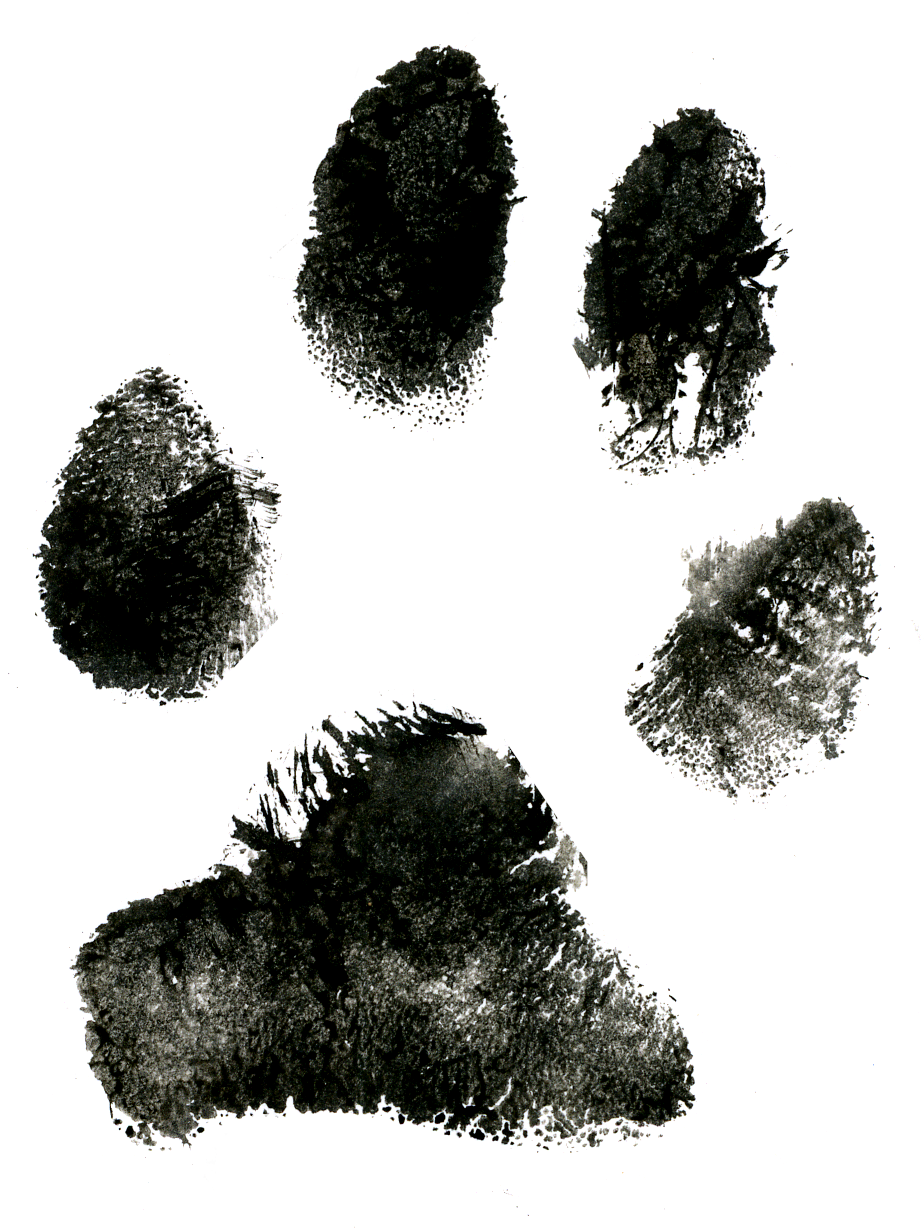
\includegraphics[width=0.5cm]{assets/zpaw.png}
  \end{center}
}

\newcommand\storydiv{
  \begin{center}
    \null
    \vfill
    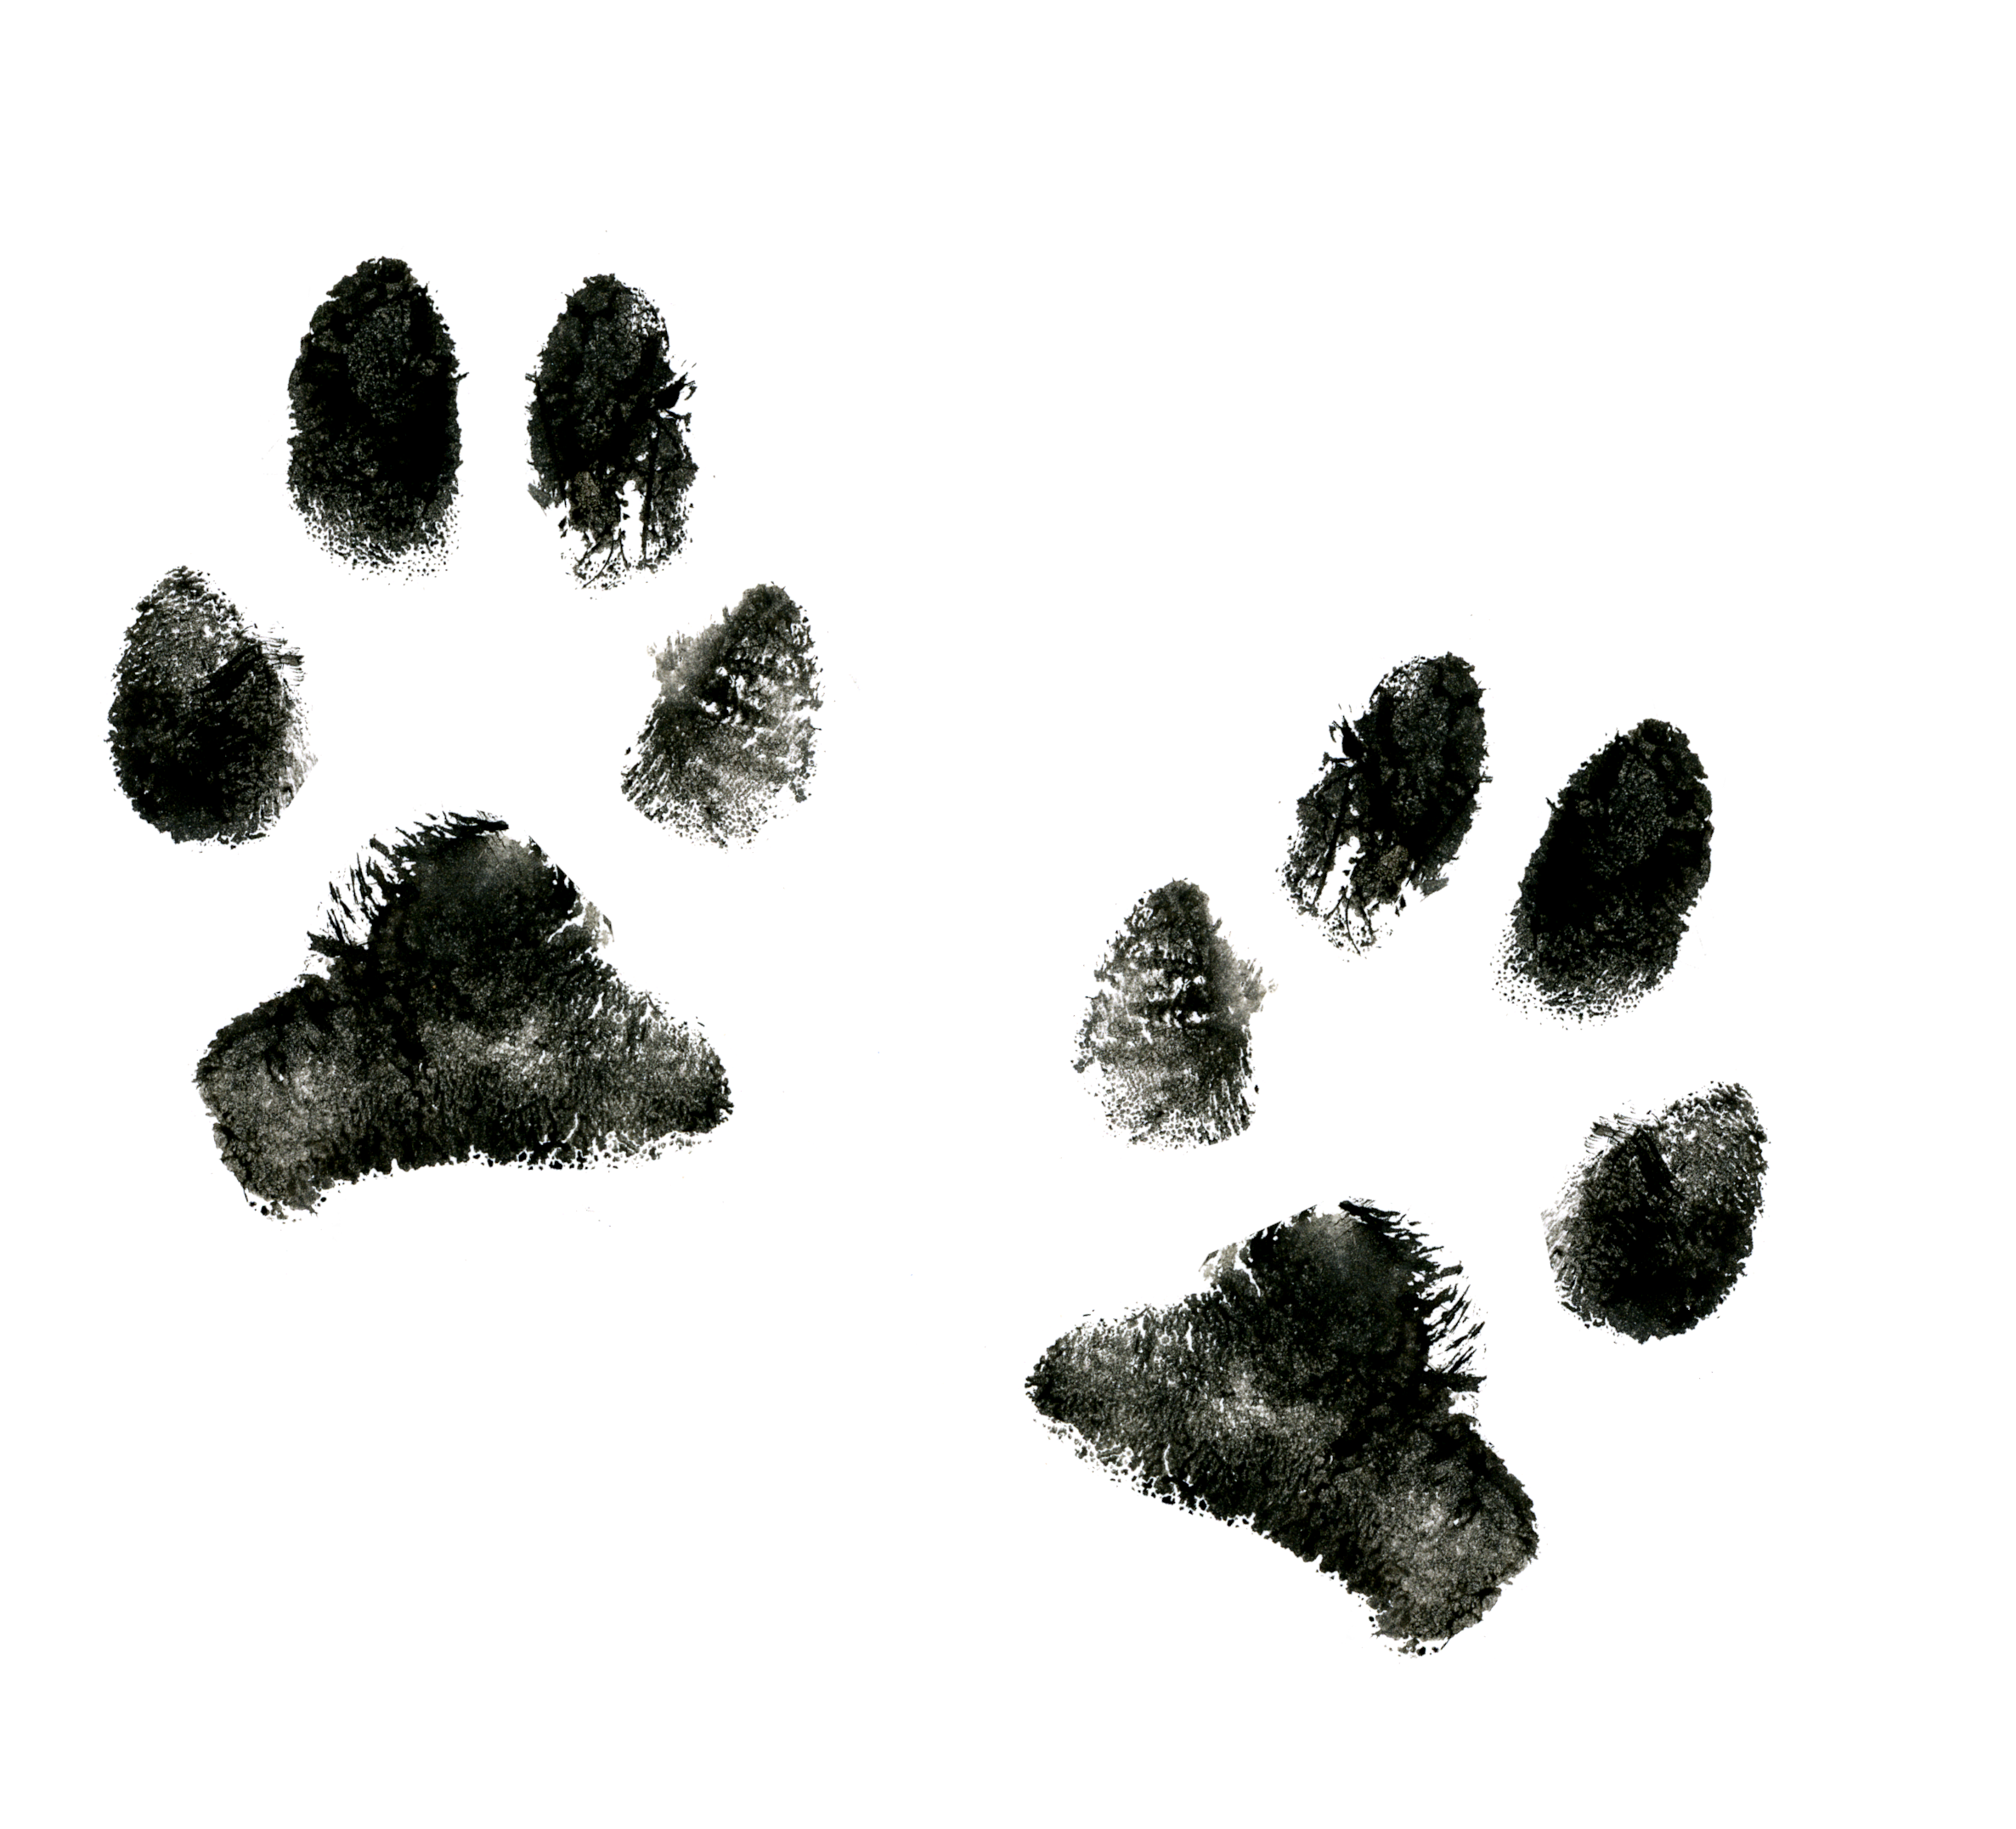
\includegraphics[width=1.7cm]{assets/2zpaw.png}
    \vfill
  \end{center}
}

\hyphenation{
\AuthorFirst
\AuthorLast
\Title
\Subtitle
}


\begin{document}
  \frontmatter

  \thispagestyle{empty}
  \null
  \vfill
  \begin{flushright}
    \DisplayFont Mitzvot
    
    \vspace{1ex}

    {\footnotesize and Selected Letters}
  \end{flushright}
  \vfill
  \cleardoublepage

  \pagestyle{empty}

  \doublespacing

  \begin{flushright}
    \null
    \vfill
    {\Huge\DisplayFont Mitzvot}

    \vspace{1ex}

    {\Large\DisplayFont and Selected Letters}

    {\DisplayFont Post-Self book IV}

    \vfill

    {\Large\DisplayFont Madison Scott-Clary}
  \end{flushright}
  \thispagestyle{empty}

  \newpage

  \singlespacing
\thispagestyle{empty}
\begin{center}
    \noindent {\DisplayFont Also by Madison Scott-Clary}
    \TitleFamily

    \vspace{2ex}

    \emph{Arcana — A Tarot Anthology}, ed.

    \vspace{1ex}

    \emph{Rum and Coke — Three Short Stories from a Furry Convention}

    \vspace{1ex}

    \emph{Eigengrau — Poems 2015-2020}

    \vspace{1ex}

    \emph{ally}

    \vspace{2ex}
    
    \textbf{Post-Self}

    I. \emph{Qoheleth}

    II. \emph{Toledot}

    III. \emph{Nevi'im}

    IV. \emph{Mitzvot}

    \vspace{2ex}

    \textbf{Sawtooth}

    \emph{Restless Town}

    \emph{A Wildness of the Heart}

    \vspace{2em}

    Learn more at \emph{makyo.ink/publications}
\end{center}
\vfill
\singlespacing
{\small\parindent0pt\parskip5pt
\noindent Copyright \copyright\ 2020, Madison Scott-Clary. This work is licensed under the Creative Commons Attribution 4.0 International License. To view a copy of this license, visit \mbox{\emph{creativecommons.org/licenses/by/4.0/}} or send a letter to Creative Commons, PO Box 1866, Mountain View, CA

\vspace{1ex}

ISBN: \ISBN

\vspace{1ex}

\textit{Nevi'im}

\vspace{1ex}

Cover \copyright\ Iris Jay, 2022 --- irisjay.net

\vspace{1ex}

%\textit{This digital edition has been posted to Internet Archive and OpenLibrary by the author.}

\Edition\ Edition, \Year. All rights reserved.

\vspace{1ex}

This book uses the fonts Gentium Book Basic, {\DisplayFont Gotu} and {\TitleFont Linux Biolinum O} and was typeset with {\usefont{OT1}{cmr}{m}{n}\XeLaTeX}.

%Printed in the United States of America\\
%\EditionsList
}%\parindent0pt

\clearpage


  \tableofcontents*
  \newpage
  \null
  \cleardoublepage

  %\onehalfspacing
  %\doublespacing

  % \null

\vfill

\noindent \textbf{Content Warning:} These stories contain descriptions of sex and sexuality. \emph{How Many} contains explicit description of mental health issues. \emph{Again} contains drug use.


  \mainmatter

  \pagestyle{ourbook}

  \cleardoublepage
  \null
  \thispagestyle{empty}
  \vfill
  \begin{quote}
    \small
    %Whatever happens, it was designated long ago and it was known that it would happen; as for man, he cannot contend with what is stronger than he.
    \emph{Whatever it is in your power to do, do with all your might. For there is no action, no reasoning, no learning, no wisdom in Sheol, where you are going.}
    %\emph{When you make a vow to your God~{\HebFont יהוה}\,, do not put off fulfilling it, for your God~{\HebFont יהוה} will require it of you, and you will have incurred guilt; whereas you incur no guilt if you refrain from vowing. You must fulfill what has crossed your lips and perform what you have voluntarily vowed to your God~{\HebFont יהוה}\,, having made the promise with your own mouth.}
    %\emph{When you make a vow to the Lord your God, do not put off fulfilling it, for the Lord your God will require it of you, and you will have incurred guilt; whereas you incur no guilt if you refrain from vowing. You must fulfill what has crossed your lips and perform what you have voluntarily vowed to the Lord your God, having made the promise with your own mouth.}

    %--- Deuteronomy 23:22--24
    --- Ecclesiastes 9:10
    %--- Ecclesiastes 6:10
  \end{quote}
  \vfill

  \part{Conversation}
  \begin{quote}\itshape
    What lives we lead we lead in memory.
  \end{quote}

  \noindent The grandest contribution offered by newborn immortality is the ever-living memories of the dead. Our lives become a ceaseless eulogy.

  \vspace{1em}

  From \emph{Ode} by Sasha
  \vfill

  \hypertarget{true-name-2124}{%
\chapter{True Name—2124}\label{true-name-2124}}

The next meeting spot for the Council of Eight was in a rooftop bar. However, given that that rooftop bar was in the midst of a block of apartment buildings and vertical malls that had built with shared walls, such that there was a cubic half-mile of stair-climbing, elevator rides---down as well as up---and trestles that bridged buildings of lower height than higher ones, it was more adventure getting to the venue than the meeting itself promised.

Still, The Only Time I Know My True Name Is When I Dream climbed.

The apartment buildings ranged from serviceable to gutted, and more than one time, she had to step carefully through a path covered in rubble. She could not decipher whether this was due to abandoned renovations, some unknown battle, or the simple degradations of time.

The malls offered different dichotomies. Some of them were sparkling new with speakers that whispered to her in Mandarin and lights that shouted in her face, while others played placid muzak through halls lit only by emergency lights, darkened storefronts yawning onto scuffed and over-waxed parquet floors.

She wondered who it was that had owned this sim, what collective it was that had decided to mash all the best and worst multiple clashing centuries worth of Kowloon Walled City and the North American Central Corridor.

And then, the rooftop bar. Despite no vehicle entrance to the complex, this was situated on the top level of what appeared to be a car park straight out of a mid-western American airport, complete with one or two of those vehicles that seemed perpetually parked, ones that had lingered for months or years, accruing a parking debt of thousands, tens of thousands of dollars.

The bar itself was a pop-up affair, with walls and ceiling of corrugated plastic held together with rivets and tape, a bar-top that was a few two-by-eights set across a trestle, fronted with further corrugated plastic to keep the patrons from kicking fridges or sinks out of alignment.

The drinks: early 2100s hipster bullshit, all intensely sweet or riddled with smoke-scented fizzy water or long strips of seaweed or clams within the ice cubes, steadily making the drink more and more savory over time.

True Name found it all confusing and jarring.

She liked it immediately.

Debarre was already at one of the tables---similarly cobbled together---sipping something that seemed to be all foam. He waved to her as she entered, and she waved back, heading to the bar to pick up one of those seaweed concoctions before joining him.

``That looks fucking gross, Sasha.''

She laughed and shrugged. ``I am True Name, but yes, it really does. If we are going to meet in a place that gives me a headache to walk through, it is probably best that I get something with\ldots protein? Is that how this works?''

``Uh, sorry. Yeah. True Name.'' The weasel splayed his ears and averted his eyes. ``Can we talk about that sometime?''

``Yes, but probably as Michelle, if that is okay.''

``Why?''

``She is\ldots closer to it than I am.''

Debarre gripped his glass more tightly and twisted sideways to swing his leg over the bench and straddle it. ``Yeah, I don't get it. Before everyone else gets here, can you at least give me a sentence or two?''

``When she forked, when I\ldots became me, she decided not to fork that part of her that suffers if that is the right word.'' True Name frowned. ``Already we are drifting further apart. The species remains, the appearance and the speech patterns remain, the \emph{mind} remains, but not that part of her that is so split. I am me, I am templated off of Sasha, because being both Michelle and Sasha at the same time was no longer tolerable.''

He shrugged, still staring down into his drink. ``I can't speak to that, I guess. But why Aw--''

True Name slammed her glass down on the table a bit harder than intended, some of the drink spilling over her hand. ``Do not say that fucking name.''

The weasel jumped at the sudden intensity, and when he recovered, he finally met her gaze. His expression softened from fear and anger to a tired bleakness. That moment drew out for a long few seconds of quiet and seething sadness. He reached for a napkin from the dispenser at the end of the table and handed it to her. ``Here.''

She hesitated, mastered a surge of unnamed emotion, and accepted the napkin to wipe the sticky drink from her paw and then, on realizing that she was crying, the tears from her face. ``Sorry, I am just\ldots{}''

``We'll talk.'' He reached over and gave her dry paw a squeeze in his own. ``Michelle and I will. There's something I'm missing here is all, and I want to figure out why more than what.''

True Name hid her muzzle in her drink and pretended to take a sip until she was sure she wouldn't slur her words when she spoke. ``Thank you. She is open to messages still, I will let you two work it out. For now, I need to focus on the meeting. Jonas and Zeke are here.''

Looking over his shoulder, Debarre nodded and turned to sit on the bench to face her again, leaving room for the other two. Jonas settled next to True Name so that they could give their speech together when the time came, and Zeke, that shifting bundle of rags and grime slid onto the bench beside Debarre.

``Good afternoon,'' the almost-face within the bundle rasped.

Jonas grinned. ``It's morning, isn't it?''

A pseudopod that may have been a hand waved the comment away. ``Time has lost all meaning. I seem to have forgotten how to sleep, these days.''

``You need a vacation like Michelle.''

There was a low rattle from the rags, and True Name imagined that must be Zeke's laughter. ``Don't tempt me. I don't have the funds to fork, so you'd be down to seven.''

``Why \emph{did} you make it so expensive?'' Jonas elbowed True Name in the side.

She held up her paws defensively and laughed. ``I did not. The price is tied to system capacity.''

``The laws of physics were a mistake and reputation is a lie.''

``It is the best limiting factor that we have that is not a complete fabrication, at the moment.''

``I rather miss coins.''

``My dad used to collect coins, you know.''

And so on, until the table was full and the cone of silence fell.

``Sasha? Uh\ldots True Name. Jonas?'' one of the well-dressed triad asked.

``Right,'' Jonas said, setting his drink down. ``The bill. Things are progressing slowly, as they always do, but it sounds like they might start picking up steam shortly. Our main contact on the DDR side, one Yared Zerezghi based out of the Northeast African Coalition, says that some of the governments are starting to take interest in the bill, which could work to our advantage. Having it just be a direct vote would mean that we would have far, far more representatives to convince, since that'd mean essentially everyone on the DDR. The more governments in play, the more the role of the DDR shrinks.''

``How does that even begin to help? Aren't they super stodgy?'' Debarre asked.

``They can be,'' Jonas hedged. ``But if we can form contacts with each of them, we can argue our case directly. Yared might be the one to give us a good in for the NEAC, and I still have some Western Fed contacts.''

``Anyone for the S-R Bloc or anywhere in SEAPAC? Middle east? India?''

The trio of suits raised their hands. ``S-R Bloc. We don't know any of the oligarchs directly, but we had some big money interests of our own.''

``Israel,'' Zeke said, then laughed at the awkward silence that followed. The trio frowned. ``Sorry, nothing to be done there.''

``And SEAPAC?''

user11824 shrugged. ``I was a nobody, but I was a Maori nobody.''

``You had enough to upload. That has to count for something, doesn't it?''

He shrugged again.

``We will take all the help we can get,'' True Name said. ``Even from nobodies.''

``Alright, I'll poke mom.''

Zeke nodded to True Name. ``What's your take on the situation?''

She stirred her drink to buy herself some time to think. ``I think it is leaning our way. One of the big arguments remains speciation, but Yared's turning that into a pro-rights argument instead of a neutral- or anti-rights one. His voice is getting louder, too. It sounds like he is getting a lot more upvotes on his posts than before.''

``That's good.''

True Name nodded. ``I think so. He is not the biggest voice on the issue yet, but it sounds like he is probably in the top three.''

``You said he's NEAC, right?''

``Yeah, Addis Ababa,'' Jonas said. ``Not exactly the seat of power, but I guess not everything has to be Cairo. Sounds like we have a good mix, at least. No one from South America?''

Everyone shook their heads.

``I suppose that's alright. They're a big enough voice in Western Fed, but they're still in the shadow government side of things. They don't even have the shadow minister of System affairs.''

``Who does?''

``Lithuania.''

One of the suits laughed, and Debarre looked blank.

``Politics,'' Jonas said, grinning lopsidedly.

``If you say so.''

After a moment's silence, Zeke rasped, ``So what are our next steps?''

``Let's all talk to our respective interests---Zeke too---and we'll meet again soon. True Name and I will keep working with Yared and guide as best we can from our side. Speaking of, though, any thoughts on the speciation topic?''

Six sets of eyes flitted between Debarre and True Name, between weasel and skunk, then the whole council laughed.

``I don't give a shit,'' user11824 said. ``But if your Yared guy can twist that argument against the opposition, then that's just one more tool, isn't it?''

``We aren't seeing that,'' the man in the suit spoke up. ``Two thirds of our power structure still think child restrictions are a good enough idea that those laws have bled into Russia. I'm pretty sure they see speciation as a positive. What better way to help in population control?''

One of his companions shrugged, ``I wouldn't be surprised if they started putting limitations on uploading by gender, but that is a separate topic.''

``Zeke?''

The pile of rags shifted in a shrug.

``Debarre? True Name? Anything you can leverage?''

The weasel laughed. ``I mean, if you want to point to us as an example to push that along, and Yared's tack seems to be working, go for it.''

``Alright. It's something you can suggest to your respective interests if you think it'll help. We'll reevaluate next meeting. Anything else on the agenda?''

Everyone shook their heads, then lifted their glasses to a toast. The cone of silence dropped.

``Well, then, you are all free to stick around or go if you want,'' True Name said. ``I am going to stay and get well and truly plastered.''

  \begin{center}\rule{0.5\linewidth}{0.5pt}\end{center}

``To be built to love is to be built to dissolve. It is to be built to unbecome. It is to have the sole purpose in life of falling apart all in the name of someone else.

``We all have a bit of that in us, do we not? You find yourself at a bar or maybe in some class somewhere, you look over, and there they are, right? You look over and you maybe catch their eye and you come undone at the seams. You fall into those big, beautiful eyes — for when you are built to love, every eye that catches yours is the most beautiful thing of all time — and you begin to flake away at the edges.

``And to be built to love is to be all edges. They catch on your clothes, they brush against walls and furniture. You are all edges so that love can fill the cracks and soften those jagged corners.

``You are spiked and barbed. It is as if you are built that way on purpose, so that the slightest breeze can blow you about and catch you up on some future love.''

\AddToHookNext{shipout/after}{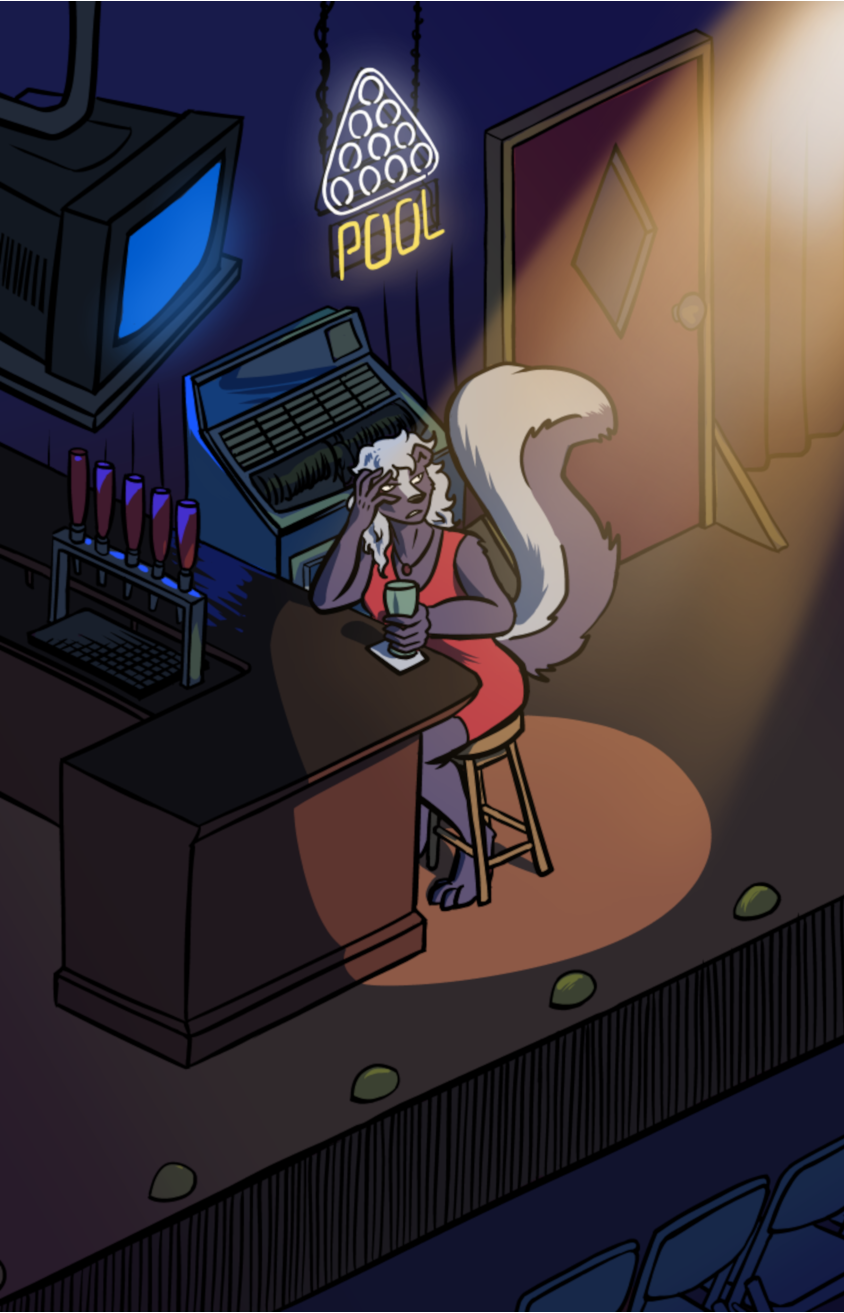
\includepdf[pages={1}]{assets/may-bar}}

The skunk had been sitting on a barstool, hunched over a pint and slurring half to the glass, half to some absent bartender. She slid to her feet, wobbled for a moment, then righted herself.

``Actually, you know what? I have heard it said so many times that to hate — truly hate, burn up inside with that passion — is to actually be in love with the object of your hatred, but I think there is a little bit of hatred in love, too. You fall so completely for someone that you just cannot help but resent them. It is a mirror of that hatred for yourself, for all your jagged edges and prickly burrs, a reflection of the resentment that you feel towards yourself for having been built to love. And look at me!'' She gestured down at herself, a grand sweep of the paw outsized in her intoxication. ``I fuckin' loathe myself! Can you imagine how deeply I must love others, then?''

After a moment's wild laughter, she stumbled back until her tail crumpled against the edge of the stool. ``Ow! Fuck. Yeah, I deserved that one, I think.''

She moved to finish her pint, frowned on finding it empty, and shuffled away from the bar.

``So yeah, you hate yourself, and it actually feels kind of good, does it not? Hatred can fill in those cracks as easily as love. Sure, it may not leave so pretty a pattern as the\ldots whatsit\ldots the patina that stains a tea cup with crackled glaze, but maybe the edges of you do not catch on so many things anymore. Maybe those prickles are dulled and you bounce off everyone around you. You can ping-pong through life, then, loving everyone and loathing yourself.''

The skunk stood up straight again, brushed her shirt out, and brought her tail around to rub at where she'd bumped it against the stool.

``Good Lord, May,'' Ioan said, laughing.

She grinned widely, all that feigned drunkenness suddenly gone from her expression. ``How was it, my dear?''

Ey slouched back against the front row seat ey'd claimed, tapping the end of eir pen against eir lower lip. ``Really, really good,'' ey said. ``Was the stumble intentional?''

``The movement itself was,'' she said. ``Though hitting my tail was not.''

``So no `I deserved that one'?''

She sat down on the edge of the stage, kicking her feet idly. ``It was not in there, no, but I think I will keep it.''

Ey grinned and closed eir notebook around eir pen, setting it aside to stand. ``Yeah, it's good in there,'' ey said, leaning forward to give the bridge of her snout a kiss. She squinted her eyes shut and then scrubbed a paw over her muzzle. ``I mean, the whole thing's good. Only note I really had is that you say `hate' four times in a pretty short span right after you stood up. `That to hate', then `truly hate', then `object of your hatred', and then `little bit of hatred'.''

``Should I make them all different?''

``I'd keep the first two because it works as an echo, so maybe just change the fourth? `Loathing'?''

``Excellent, O great wordsmith.''

Ey laughed and tweaked her ear before hoisting emself up onto the edge of the stage next to her. Predictably, she scooted closer so that she could lean against eir side. ``Who would've thought, hmm? You getting me into theatre and me getting you into writing.''

``This is still theatre! Just earlier on in the process,'' she said, indignant. ``But yes, it is proof that the Bălans can shove us around instead of only the other way around.''

Ey gave her a playful shove with eir shoulder, at which she let out an outsized yelp followed by a whimper. ``So mean!''

``Yeah, that's me. Meanest person you know.''

She rolled her eyes.

Ey let a long silence play then, looking out into the cool darkness of the theater while May summoned up her notebook and scribbled down eir tip from earlier.

``Do you really feel that way?''

``Mm?''

``The jagged edges and self-loathing.''

She shrugged. ``There is some of me in there, yes, but it is still theatre. It is about taking the particular and making it universal, if only for a little while, yes?''

Ey nodded.

When ey didn't reply otherwise, she shrugged and continued, ``I would not say that I agree with that `I loathe myself, so imagine how much I love others' bit. I do not loathe myself, and yet I still love others. Have loved and will love in the future, even, and I see no change in my rare moments of self-loathing.''

Ey laughed. ``\,`Will love in the future'? You leaving me for some handsome guy you met in a bar, then?''

``A bar? Ugh. I am apparently more of a `hunt nerds in the library' type.'' She poked em in the belly. ``But I love \emph{you}, Ioan, and will continue to do so.''

Rubbing at the spot where she'd poked with her dull claw, ey nodded. ``Love you too, May.''

She beamed happily and settled back in against eir side, head resting on eir shoulder. ``I am glad, my dear. I know we agreed early on that this — us being together, I mean — does not need to be permanent, but that does not change the fact that I will continue loving you. Even if we should split, I will not stop.''

Ey nodded slowly.

``I have no plans for such,'' she added quickly. ``You are stuck with me for a good while yet.''

``What? Oh, no,'' ey said, shaking eir head to clear a few too many thoughts. ``I trust you on that. Just got me thinking. Do you still love all the others you've been with?''

She laughed. ``What I said does not apply just to you. Of course I still love them. Some long-diverged forks of me are even still in relationships with their partners.''

``So you've said. You still love them as the root instance, though?''

She nodded. ``I do not begin relationships as anything other than my root instance. I do not know why, but it does not feel fair of me to do anything but.''

``Oh, so none of your forks went on to fork for other relationships?''

``Not that I know of, no. It is a firm conviction, so I would imagine that they hold to it, but perhaps some older ones have diverged. We do not speak much.''

``How many are there, anyway?''

She lifted her head to dot her nose against eir cheek. ``Are you jealous, my dear?'' Her voice was calm and curious. Calm enough and curious enough, some distant part of em noted, that it kept em from falling immediately into defensiveness.

``I get the occasional pangs, more so early on,'' ey said after a long moment's thought. ``When ey was first getting settled in eir relationship, Codrin told me about something that Dear had told em shortly after ey'd been forked, `jealousy is a sign of needs not met'. Whenever I start feeling jealous, that's usually a sign for me to take a step back and think about what need that might be.''

``See, this is what I like about you, Ioan. You feel a thing and then think about it until you understand it. Sometimes a little too much, but it has served you well.''

Ey tilted eir cheek to rest it atop her head, a bit of closeness that also served the purpose of stopping her ear-tip from tickling eir neck.

``I feel a thing and am helpless before it. I cannot but wrap myself up in\ldots it\ldots{}'' she said, pulling out her notebook again to jot down the words as they came. ``Love, hatred, hunger, exhaustion. I am built for them all, and I cannot do a thing about them\ldots{}''

Ey shared a secret smile with emself as the skunk trailed off, continuing to write, tongue-tip peeking out from her muzzle.

``Also,'' she said once she'd finished. ``The answer is that I do not know how many of me are still in relationships. There are at least three, and I know of at least five that have quit, though I declined the merges out of privacy. I never made it a requirement that they keep in touch. Beyond that, I think there are\ldots mm, seven, perhaps?''

``So that makes me your sixteenth relationship?''

``Something like that, yes. Sixteenth truly serious one.'' She slid over and swung her legs up onto the stage so that she could rest her head in eir lap. ``Did my monologue really get you thinking about all this?''

``It's a good monologue,'' ey said, petting over her ears. ``Or start, at least. You said it should be five minutes, right?''

She nodded. ``Around that, yes. I am still working on it.''

``Mmhm. It's good so far, though. It got me thinking, but I'm also just fascinated by you, which helps.''

``Why, because I am weird? I think that is an Odist thing,'' she said, laughing.

``What, am I not allowed to be fascinated by my partner?''

``Absolutely not, no.''

Ey tugged on her ear. ``Fascinated and annoyed.''

``Yes, well, too bad. You remain stuck with me, Mx. Bălan.'' She continued more seriously, ``I did not expect this to be fascinating to you. I try to be careful talking about my other relationships.''

``I don't really mind,'' ey said after giving it due thought. ``That was past May, right? It'd be like getting upset over someone else having exes. If it were multiple partners at the same time, that'd probably be a separate conversation.''

She shook her head. ``I could not do that. I am not built the same as Dear. I am only in multiple relationships in the sense that there are multiple mes, but there is only ever one me involved with one other. It is parallel monogamy.''

``Why?''

``Because,'' she said, rolling onto her back so that she could smile up to em. ``I am also helpless before devotion, and that takes the whole of me.''

``What about Douglas or A Finger Pointing?''

``I hold no romantic feelings for A Finger Pointing.'' She laughed. ``She is nice, but in a boss-you-drink-with-on-Fridays-and-I-guess-occasionally-have-a-fling-with sort of way.''

``And Douglas?''

Her answer was a while in coming. ``Were our friendship to head in that direction, I would fork, but I do not foresee that being the case.''

``Really?'' Ey frowned. ``Wouldn't that be awkward? Us going over there to see him and the other you together?''

``Oh, incredibly awkward,'' she said, rolling her eyes. ``I have done similar in the past, and it would take a year or two to shake out. It is uncomfortable for me, as well, as I am left with the same desire even as my down-tree instance gets fulfillment and they are left with love for you.''

``I can imagine.''

``No, Ioan, I do not think you can,'' she said primly. ``You actually think about the way you feel as you are feeling it like a normal person rather than just crashing headlong into overwhelming emotions like a fucking Odist.''

``Well, fair.''

``I do not think we need to worry about that, though. I am comfortable with my friendship with him just as I am comfortable loving you, and should someone catch my eye--''

``You'd need to start going to more libraries, I think.''

She laughed and shook her head, continuing, ``--should someone catch my eye — or yours, for that matter — we will tackle it then with plenty of talking.''

``Oh, I believe you on that. Skunks never shut up.''

She made as if to bite em on the belly and, when ey flinched away, grinned up to em. ``Mx. Ioan Bălan, you are the one asking all the questions with long, involved answers. Do not pin this on me.''

``Yeah, yeah. You just got me thinking is all. I think you're giving me too much credit saying someone might catch my eye, though.''

``Why?''

Ey shrugged. ``I'm not exactly that observant.''

``You worked as a professional observer for, what, a century?''

``Not \emph{that} kind of observation.''

She laughed. ``Well, okay, yes. I will not discount the possibility, though. If we are in this life for yet more centuries, there is no harm in being deliberate. Plus, I will get an inordinate amount of satisfaction out of seeing you fall for someone. It was so wholesome the first time! I see no reason why it should not be the same subsequent times.''

``I guess. I don't know if there's anyone who--''

She waved a paw dismissively. ``If there is not, there is not. We can speak in hypotheticals like fucking grown-ups.''

``Fine, fine.''

When the silence drew out, May grabbed one of eir hands and started mouthing on eir fingers, sharp skunk teeth just pricking skin.

``Ow!'' Ey laughed and tapped a finger on her nose lightly. ``Pest.''

She licked at eir fingertip, saying, ``Thank you, my dear, in all earnestness. It makes me happy to be able to have a conversation about this.''

``Of course, May. I figure it ought to be an open topic for us.''

She nodded and stretched out on the stage. ``Agreed. We can come back to it later, though. I would like to run this through once more,'' she said, waggling the notebook at em. ``And then head home to get ready for dinner. Debarre is coming over and I plan on flirting with him outrageously in front of you all night long to see if I can make you jealous.''

Ey laughed and pushed at her until she sat up before sliding off the stage and walking back to eir seat. ``Alright. Once more, from the top.''

  %\hypertarget{codrin-bux103lan-2346}{%
\chapter{Codrin Bălan — 2346}\label{codrin-bux103lan-2346}}

It took both both eir partners to talk Codrin down from eir desire to simply get right to work.

\emph{``My dear, if, as he said, Tycho was going to take a nap, perhaps you ought to do the same.''}

``I know,'' ey replied, shoulders sagging. ``It's hard to get out of that mindset of having to just work.''

``I know it's enjoyable,'' the fox's partner said. ``But seriously, Codrin, even if you're not going to take a nap, take a thermos out onto the prairie and walk for a bit. Tycho is going to need quite a bit of help, given what you told us of him--''

\emph{``And if True Name is already involved.''}

``That too, yeah. So it's probably best to go into the whole thing prepared for jittery astronomers and\ldots well, whatever True Name is, these days.''

Codrin nodded. ``That makes sense, at least. Do we even have a thermos?''

``Probably. I'll go digging. Might as well make a fresh pot, while I'm up.''

\emph{``You, my love, are a true delight,''} Dear said, tail flitting this way and that.

They grinned, walked off to the kitchen, and started clattering around in cupboards for a coffee therm.

``Dear, have you talked to True Name recently?'' Codrin asked after a polite pause.

It shook its head. \emph{``Not in terms of a conversation, at least. I have received a few messages from her in the intervening years, several of which were sent to several Odists as a group.''}

``She does that? What are they? Orders or something?''

It shook its head, ears flapping slightly at the movement. \emph{``No.~Or, well, not exactly. They are simply updates, or replies to other, ongoing conversations. Many of us still communicate with each other on a somewhat regular basis, and I have been looped into several of those conversations over the years.''}

``Wait,''not exactly``?''

\emph{``You have met her. She does not need to order, oftentimes. She simply suggests.''}

Ey frowned. ``I sometimes worry that we've been attributing almost magical manipulative abilities to her, honestly.''

Dear shrugged. \emph{``Perhaps, but she also has had more than two hundred years of study under her belt to find all of the best ways to interact with people. May Then My Name was something of a let-down for her, I think, even from the very beginning, so she had to learn to take on that mantle herself.''}

``Especially over the last few years, you mean? With Ioan?''

\emph{``Perhaps, though I think that might be ancillary to the fact that our dear May is not on the LVs at all.''}

Ey blinked, laughed. ``Okay, well, fair. I'd almost forgot.''

The fox gave em a strange look. \emph{``You forgot that May Then My Name was not here?''}

Their partner showed up, a cup of coffee in one hand and a (far too large) thermos in the other. ``Are you forgetting things again, Codrin?''

``No, no,'' ey said, accepting the thermos with a frown. ``Or, well, kind of. I didn't forget that May Then My Name wasn't here, just the ramifications of that, that True Name might not have her as a tool.''

\emph{``That is more understandable, yes,''} the fox said. \emph{``Perhaps the True Name here on Castor has diverged from that on the L5 System in that respect, perhaps not. I suspect that both are disappointed, in their own ways.''}

Codrin fiddled with the thermos, ensuring that the lid was a mug when removed — two nested ones, actually — then nodded, standing. ``I don't know how many dimensions she's thinking on, but I also wouldn't be surprised if she had a cost-benefit analysis on losing her to Ioan.''

\emph{``I would not be surprised, no, which would mean that she has planned around that eventuality. I am sure that May Then My Name is keeping an eye on that. Do not let us keep you, though, my dear. Go for your walk. Think about something else. Enjoy the cold, build a cairn around your worries, and then return safe.''}

Ey smiled, leaned down to kiss the fox between the ears, then eir other partner on the cheek. ``I didn't know that was possible, but I'll try. Back in a bit.''

Ey made it two cairns out before caving to the desire to simply get started, and stepped over to Tycho's field. There was a ping of amusement from Dear, to which ey replied with a guilty apology and an acknowledgement that ey'd return soon, all while waiting for eir eyes to adjust to the sudden darkness.

The next sensorium message was a gentle ping to Tycho — nothing so loaded with anxiety as the one ey'd received this morning, just an acknowledgement, a view of the stars.

A voice came from somewhere behind em. ``Codrin?''

Ey whirled around to see a dim cone of red light shining on the ground, illuminating feet in a pair of well-worn boots. ``Tycho? Sorry for intruding like this. I hope I'm not waking you or anything.''

``No, no. Come in. I haven't been able to sleep since True Name left.''

There was a small click and then a ray of further red light spread out from a doorway, showing a small hut nestled within the trees. Ey let emself be guided into the door, finding a sparsely decorated room — a desk, a bed, and a massive cork board nailed to the wall, covered in at least three overlapping layers of notes.

``Thanks for having me,'' ey said, sitting on the offered chair while Tycho claimed the edge of the bed. Once the door was shut, a switch shifted the red light to a normal, warm desk lamp. ``I should've mentioned that I'd be coming over, first.''

He waved away the apology. ``I knew you'd be here, though I didn't know when.''

Codrin paused in the middle of unscrewing the lid to the thermos. ``You knew?''

``True Name said you would.''

Ey frowned, finishing opening the thermos and offering Tycho one of the two mugs of coffee. ``What did she say about me?''

``She didn't talk with you?''

Ey shook eir head. ``Did she say she would?''

Tycho sipped at the coffee, winced, and set the mug aside to cool. ``No, she just talked as though she had, or at least that she knew you'd be working with me.''

``Of course she did,'' ey murmured. ``She knows me too well.''

The astronomer ground the heels of his palms against his eyes. ``I feel like she knew me too well, too. We had what felt like a wonderful conversation where she offered me a job, asked me to fork to send an instance with her to keep working with her, but then quoted some bit of poetry at me and I couldn't tell if it was a death threat or a warning or whatever. I'm still trying to recover from that.''

``I'm guessing you said yes to both the job offer and the fork?''

He nodded. ``It all just sounded so normal. There didn't seem like anything else to do.''

``Can you tell me more about both?''

``Well, she said that she a good deal about the communications and that she'd like me to come help her with the mechanics of that. She'd help me out with resources and I'd teach her about Artemis as I learned it.''

``Artemis? Is that what they're calling the remote\ldots ship? Vehicle?''

He nodded. ``Vehicle, I think. She said they're calling it Artemis, that I should tag my fork \#Artemis, and that those on the ship were either Artemisians or Sea People, which I didn't get.''

Codrin leaned back in the seat, thinking. ``Sea People might be a reference to something from the Mythology, or it could be a reference to a theory about a marauding group of seafarers during the Bronze Age collapse. There was a bunch of talk about how this group had sacked much of the ancient near east and northern Africa, leading to the prolongation of the collapse.''

Tycho's eyes grew wide. ``Do you think that's what she's getting at with the reference? That these are going to be some marauders coming to mess with the LV?''

Ey shrugged. ``Who knows. Probably both, honestly. Maybe there's even some reference that we're missing. She's True Name, there really is no way of telling.''

Nodding, Tycho scooted back on the bed until his back was to the wall, then brought his knees up to his chest. He looked small to Codrin, somehow diminished after the events of the last\ldots goodness, had it only been a day? Diminished, yes, and younger, though he'd always looked as though he was not yet out of his forties in his well-groomed salt-and-pepper hair and well-kept beard.

They sat in silence for a while. Codrin could not guess what the astronomer was thinking about, though ey could see his eyes occasionally darting this way and that, as though connecting one idea to another in the air as well as in his head.

On eir part, ey began structuring the project. There would have to be the journalistic aspect of it, much closer to that of the Qoheleth project than the History, but if the conservative Odists were also involved, there'd likely also be far more observing than researching.

``Tycho,'' ey said, startling him out of a reverie. ``Do you know what an amanuensis is?''

``Like a recorder? Someone who takes notes?''

``Well, in part, but also someone who thinks about what they're writing,'' ey said, tapping at eir temple. ``They aren't a scribe or a court recorder, but someone there to witness and digest a conversation.''

``Like a clerk?'' He grinned. ``We used to have one of those for our club, who would take minutes of the meetings and such.''

Ey nodded. ``Certainly closer to that than a recorder, yeah. I bring this up because that will be my job in all of this, but I think it'll also be yours. Things like the History are all well and good, and I loved putting the work into it, but I also really enjoy doing this. I may wish that the things I get caught up in weren't always so dramatic, but I'll take what I can get.''

``What do you mean, it'll be my job too?'' he asked.

``Just that you will also be witnessing and thinking about this project, and then coming up with ideas related to it to be compiled into a coherent understanding. That's why we'll be working together, I think. I'm trained to do this work in particular, but I'll need your help in making sense of it. I'll experience it with you as much as I'm allowed, but you'll have to ensure that I actually understand what's going on.''

Tycho laughed. ``Well, I'll do my best, but it's not like I have much experience working with Artemisians, either. I'll help with the technical aspects as best I can, though.''

``Excellent,'' Codrin said. ``Thank you for that. I'll be managing most of that, so you won't have to worry too much about the minutiae, but I figured it'd give you a better idea of what to expect when we work together.''

He nodded.

``On that note, lets come up with a basic idea of our next steps. We mostly talked about immediate next steps, but it might be a good idea to start thinking on a larger timescale.''

``I guess. I'm assuming it'll be pretty loose, given that we can't guess the particulars?'' He waited for Codrin to nod, then continued. ``Then I guess we have a few weeks before they reach their closest approach as long as we both stay on our own heading.''

``Does that mean a few weeks before they upload?''

He shrugged. ``Not necessarily. They can upload whenever they want, so long as our Ansible is on and the DMZ is ready. I don't think it's on, yet, though.''

``Alright. Have we received any further communications from them? Their message said that they had a similar mechanism in place. Is that something we'll be able to use? Or even want to use?''

``No further communications that I know of,'' he said. ``But True Name said that all communications will be gated through her, and I don't know if that means that I'll be getting them or just Tycho\#Artemis. Hopefully both, if you and I are to be working on this as well.''

Codrin frowned. ``Well, okay.''

``As for us using their mechanism, I guess it depends on if it's something we can reconfigure our Ansible to use, or if we will need to construct something new. If we'll need to construct something new, then we might not be able to do so in time. Our manufactories are meant for repairs rather than construction. Theoretically they could be used for such, but I don't know how long that'd take without someone phys-side to help.''

``And would we want to?''

``That feels like a question for True Name, not me,'' he said after a long pause.

Ey finished eir coffee and replaced the cup on the cap of the thermos. ``One of us will have to work up the courage to ask her, sometime. But for now, is it something you would want to do?''

``What? Upload to Artemis?'' He looked startled by the question.

``Yes. If it's possible, I mean. I figure it could just be an instance rather than completely investing, though I'd also be curious to hear your opinions on that.''

Tycho tilted his head back until it hit the wall of the hut, staring up toward the ceiling. He sat like that for a good five minutes, during which Codrin remained silent, before leaning forward to grab his cup of coffee now that it had cooled down. ``Yes. I don't know that I'd invest completely, but yes, I think I would. Would you?''

Ey smiled, though ey felt just how tired ey was as ey did so. ``Perhaps. I have attachments here, though. So the Codrin who uploaded — if ey remains a Codrin — would be severed completely from those ey loves. As romantic as the idea of sailing away on some alien spacecraft might be, it'd be painful to leave, even knowing that a Codrin remained.''

``And if your partners uploaded with you?''

The thought caught em up short, and several trains of thought crunched to a halt within em. ``If they\ldots{}'' Ey laughed, shaking eir head. ``You know, I hadn't considered that, yet. I wonder why? But yes, if they chose to do so, then yes, I'll go with them.''

The conversation wound on from there, picking apart a few possible next steps that lay ahead of them, but throughout it all, at least one thread of eir mind was dedicated to picking at that question.

Why had ey not considered whether or not Dear and its partner would want to upload? It wasn't as though ey didn't attribute the agency to do so to them, ey knew just how independent and intelligent they were on their own. Nor was it that ey hadn't made any guesses as to whether or not they would — ey suspected that Dear would jump at the opportunity.

The root of the issue lay within emself, ey knew. Why was ey not able to make that decision without them doing so first? Was ey really such a follower? Or, to put it in a way that was more kind to emself, was ey really so stuck living five minutes behind them that ey couldn't imagine making the decision in the face of the possibility of simply reacting to it? Would ey be able to say yes or no to that question if they asked?

Would ey be able to argue one way or the other, to convince them to come with em or not?

  \hypertarget{ioan-bux103lan-2346}{%
\chapter{Ioan Bălan — 2346}}
\markboth{Ioan Bălan — 2346}{}

\begin{center}
\emph{Convergence T-Plus 28 days, 13 hours, 35 minutes}\\
\emph{(Castor--Lagrange transmission delay: 30 days, 14 hours, 36 minutes)}
\end{center}

\noindent Ioan knew what was coming, so ey was able to brace emself well enough when May came barrelling out of the default entry point on the dandelion-ridden field that ey was not totally bowled over, managing at least a somewhat graceful descent to the ground. The skunk had already looped her arms around eir middle and tucked her head up under eir chin before ey was even able to sit up straight enough to get eir arms around her.

``You nut.'' Ey laughed, reaching up to tug at one of her ears affectionately. ``Good to see you, too.''

``Ioan, I am in no way sorry for knocking you over,'' she said, voice muffled, her grip around eir middle tightening. ``Though I am dreadfully sorry that this happened again. I missed you.''

Giving up on the prospect of sitting up straight, ey leaned back onto one hand, propping emself up. ``No need to apologize, May. I'm just happy to see you again.''

The skunk leaned away from em enough to dot her nose against eirs. Her eyes were quite red and ey could see tear-tracks in the fur of her cheeks. She looked a mess. ``Do not take my apology away from me. I have been saving that one up.''

``Alright, alright,'' ey said, pressing eir nose a little more firmly to hers for a moment before leaning back again. ``Apology accepted. Are you feeling better?''

She sat upright rather than leaning against eir front and nodded. ``Yes. I was able to get a lot out that I think has been pent up for a while. Thank you for giving me the space. I promise I did not fuck with your pen collection.''

``Good. I had it all perfectly organized.'' Ey plucked a dandelion from the field and tucked it behind her ear. ``Now, do you want to talk about it? Or should we do that later? That was longer than the last few times.''

``Later, please. I want to say hi to Douglas and wash my face and just be normal for a bit.''

Douglas Hadje met them on the stoop of his house and, as had become their ritual over the years, hugged the skunk, lifted, and twirled her around. Her bushy tail streamed along behind her.

``Hey May,'' he said, setting her back down again and kissing her cheek. ``Glad you made it through.''

``Of course I made it through. You still have at least seventy nine years of me haunting you before I can do something else.'' She grinned. ``And even then, the contract is renewable.''

``Ornery as ever.'' He laughed. ``Well, want to come in?''

``For a bit, and then I want to come back out here and lay in the grass and bake in the sun.''

After May had cleaned up and Ioan had helped Douglas prepare coffee and some sandwiches, they sat around the table to catch up.

``So, what news of the aliens?'' Douglas asked.

The skunk squinted at him. ``Has Ioan not been keeping you up?''

``A little. Ey said ey wanted to wait until you got here, though.''

``Whatever.'' She rolled her eyes. ``Well, out with it, then.''

``I've gotten several messages from Codrin over the last few days. Ey said they would be heading out to start the talks in, uh\ldots five days.''

``So they have been into them for a while, now.'' She looked thoughtfully up to the ceiling. ``A few weeks, perhaps?''

``Or maybe they're already over,'' Douglas said.

``A gloomy thought. I would like to hope that they are going quite well. Codrin is there being a Bălan, Tycho is there being a nerd, this Sarah Genet is there being a whatever a Sarah Genet is like, Why Ask Questions is there being a shithead.'' She wrinkled her nose. ``And True Name is doing her best to control the whole thing.''

Ioan was pleased to see the mildness of the skunk's expression. It really did seem like many of those overwhelming emotions had burned themselves out over the last few days.

``It's weird,'' Douglas said. ``Every now and then, I'll hear about something from one of the LVs that's anchored to a certain time and I'll remember, `Oh shit, yeah, they're billions of kilometers away by now', and then I have to spend some time trying to conceptualize that distance.''

Ioan nodded. ``The transmission delay throws a wrench in things, doesn't it? I was just thinking about that on Secession day. We were celebrating and it sounds like they were, too, but we didn't learn about their party until a week later.''

``The thing that always catches me off guard is that our days do not seem to line up any longer,'' May said around a bite of sandwich. ``I mean, they do, but when the delay is off by half a day, we start getting messages at shit o'clock in the morning. It is a strange feeling.''

``Exactly.''

``I hope they're still in the talks, too. Codrin sounded hopeful, at least. The messages that they'd been getting from the Artemisians were interesting, especially the language snippets. I'm guessing the powers that be made em promise not to send the full message text yet, but what they have learned is fascinating. Four races on one ship must be a hell of an experience. The DMZ sim sounds pleasant, though, and all of the work they've done to prepare is really kind of impressive.'' Ey sipped eir coffee to buy a moment's time to think before saying, ``There was a bunch of stuff in there for you, too, May. We can go over that later, though.''

The skunk frowned, finished the last of her sandwich, and then settled back in the chair with her coffee. ``You cannot leave me hanging, my dear. May I at least have a preview?''

``Well, Codrin's worried about you. As is Dear.''

``The memory thing?'' Douglas asked.

Ey nodded.

May averted her gaze, looking out the window to the rolling field beyond. ``I am worried, too. You know that.''

``I know. Reading between the lines, though, I think ey's worried about the whole clade. Ey's worried about you and Dear, and ey's worried about how True Name and Why Ask Questions are going to act through this. Dear reacted poorly to the whole time-modification thing.''

She nodded and sat in silence for a minute before setting her cup down. ``We are not doing as well as many of us would like, no. I have news as well, but I would like to share it outside where I can sit in the sun and feel the grass. Is that okay?''

Ioan and Douglas collected plates and coffee cups, then the three of them trooped out into the field while May spoke.

``We have lost May One Day Death Itself Not Die and I Do Not Know, I Do Not Know. Death Itself stopped talking, and then she stopped moving. In Dreams visited for a while there, and a few days ago asked me to come visit as well. That is why this spell seemed to last longer than usual. Evening hit, she smiled at us, shrugged, and then quit.''

May's voice was thick as she continued. ``They all lived in the same house, did you know that? All ten of that stanza. Many of them did not even talk with each other, and none of them ever forked. They were always quite unstable. The next morning, I Do Not Know was gone, and Names Of The Dead said that she had quit shortly before sunrise.''

Ioan and Douglas remained quiet as they walked. The skunk didn't seem to be quite done saying the things that she needed to.

She continued after a few minutes of mastering emotions, voice clear once more. ``In Dreams and I talked quite a bit. She said that there have been fewer instances of instability in older clades than expected, given \emph{On the Perils of Memory}. Fewer uploads are susceptible to the long-term effects of unceasing memory than expected, I guess. I was pleased to see that Debarre seems to be doing well.''

``That's heartening,'' Douglas said. ``At least in a way.''

The skunk nodded. ``I am pleased that the System is more stable than feared, but I am unhappy that we seem so strongly affected. In Dreams said that she is going to do some research and see if there are ways that we can at least improve on the way we deal with the effects. I do not know that there is a way to get rid of them entirely, at least not without further individuation, but the least we can do is help keep ourselves sane for longer.''

Ioan took her paw in eir hand and lifted it to kiss the back. ``Please, yeah. If you lose it, I'll be furious.''

She laughed and gave em a pitying look. ``Mx.~Ioan Bălan, you are pretty good at acting furious on stage, but I do not believe for a second that you could actually feel that way. Even Codrin was able to have a normal meeting with True Name after she did as she does with em.''

Ey did not laugh. Neither, ey noted, did Douglas.

``I am sorry,'' she murmured, ears laid flat.

``\,`Furious' is the wrong word, May. I'd lose my damn mind.'' Ey took a shaky breath and rubbed at eir face. ``I can't tell you you're not allowed to or anything, since I know it's not really up to you, but please at least try to stick around.''

``I'm not going to pile on or anything,'' Douglas said. ``But I will say I'd be pretty upset, too, so if there's anything I can do to help, I will.''

May dragged them both to a stop in the field. Her expression started out angry, then screwed up into sadness, and finally settled on tired. ``I love you both and I promise I will do what I can to stay here, stay grounded. I cannot speak for the rest of the clade, and certainly not for Dear to soothe Codrin's fears, but I will do what I can.''

It was not uncommon for these reunions to be tearful, Ioan knew, but it was a different sort of pang that settled in eir chest with the news, and it was a few minutes before ey was able to speak again. ``Sorry, you two.''

The skunk stuck her tongue out at em. ``I will allow you this one apology, but do not make a habit of it. You are allowed to cry at sad shit.''

Ey rolled eir eyes and shoved at her.

``Well, I was promised laying in the grass and baking in the sun,'' Douglas said. ``So come on, we can at least enjoy the rest of the afternoon.''

  \hypertarget{true-name-2124}{%
\chapter{True Name — 2124}\label{true-name-2124}}

It had initially taken some getting used to, meeting with one's up- or cross-tree instances. Michelle, in her role in helping associate the reputation markets to the cost of forking, had certainly done it a number of times before, but, as the cost of a new fork was only applied five minutes after it had been created, all of her forks to date had been short-lived in order to conserve her reputation for some imagined future date.

The date had come and gone, now, so True Name — and likely all of the other Odists — had had to learn how to interact with the other copies of Michelle Hadje/Sasha that had sprung so quickly into being and immediately began to diverge.

The fact that those who matched Michelle and those who matched Sasha were evenly distributed had helped at first. There had been some oddness in talking to a Michelle-alike, given the countless memories of the constant shifting between the two forms, but that had had a different flavor to it than talking to another Sasha-alike. Seeing a form and a face that so clearly mirrored her own was not exactly unnerving so much as uncanny, and the feeling had been titillating at first.

As the days and weeks went by, however, the forks diverged further and further, and different cares painted different faces, different habits were formed and dropped, and it became less like talking to an alternate version of oneself and more like talking to a twin, a sibling.

So it was when The Only Time I Know My True Name Is When I Dream met with That Which Lives Is Forever Praiseworthy.

Her initial impression is that the other skunk had shifted her wardrobe to look more professional, choosing a loose-fitting pantsuit in muted blue that had been in style before Michelle had uploaded. This also included a pair of pince nez glasses perched atop her muzzle which, when True Name inquired, Praiseworthy explained were non-prescription, and ``something I am just trying for the moment. They are quite annoying, but still fetching.''

Beyond that, however, Praiseworthy had decided to divest herself of many of the personality traits that had made Sasha Sasha. Gone were those aspects of childishness that Michelle had long held onto, and gone was the exhaustion that had lingered for years after getting lost.

\emph{I have changed, too, at that,} True Name thought. \emph{I have become the politician, working with Jonas. Praiseworthy has become something else.}

The two skunks shook paws, and then Praiseworthy drew True Name into a hug. It was surprising, but something about it felt both natural and performative, as though this was just a thing that one did when one had a role to play.

``True Name,'' Praiseworthy said. Her smile was warm and earnest, and she spoke with willing paws, palms up. ``It is nice to see you again.''

She laughed. ``I suppose so. You have changed quite a bit in so short a time.''

The other skunk bowed, laughing. ``As have you, my dear! And that is why you have come here, is it not?''

``I guess it is, yes. The more I work with Jonas, and the more I talk with the Council and phys-side — the more politicking that I do — the more I feel the ways in which my attitude and expressions are lacking.''

Praiseworthy nodded. ``Yes, you do still have some of the stiffness about you, and there are some sharp edges that could do with softening.''

``Softening?''

``Yes. It is mostly a matter of appearance and affect, though. You should not blunt your wit or intellect, just your words and features.''

True Name frowned. ``I am not sure what you mean by blunting or softening, though.''

Praiseworthy took her gently by the elbow and started walking through the grass. They had decided to meet on a portion of Michelle's dandelion-ridden sim, far away from their root instance, but in a place that was still familiar to both.

``Take your walk, for instance. Even now, as we are just out for a stroll, you walk with purpose. Your shoulders move too much. Remember, if you keep them pointed straight ahead and shift the rolling motion to your hips, it will lead to others seeing more feminine aspects in you.''

She tried to keep her shoulders still as they walked, immediately feeling a slight strain in her hips.

Praiseworthy laughed. ``You do not need to keep them level to the ground, just perpendicular to the direction you are walking in. But here, no need to practice too hard. Fork, holding in your mind a pelvis just a hair wider than your own, but keeping your hips the same width. It will mean slimming down a little.''

``I can do that?''

``Of course. Zeke dreamed some algorithmic magic behind the scenes, but you can fork yourself into most anything that can be consensually held in the mind.''

True Name nodded warily, holding this new image of herself in her mind.

``Excellent,'' Praiseworthy said, moving to take this new fork by the elbow and nodding to the original instance of the skunk. ``Now you quit. No need to incur a charge. Michelle, no need to accept further memories for a bit.''

The skunks tilted their heads in unison.

``Michelle will be getting a pile of memories, if she wants, as I will have you fork a few more times yet. I have been letting her know when she can ignore further merges, as I have done this quite often.''

The first True Name nodded, then disappeared.

True Name nodded, taking a few more steps and finding it far easier to walk casually and still keep her shoulders pointed forward. She nodded approvingly. ``What other suggestions do you have?''

``For your role, you will need to carefully balance cute, attractive, and competent. If you go too far towards cute, then it will be difficult for you to be taken seriously. The same if you go too far attractive because you will be just a pretty face. If you go too far competent, you will be seen as dour and unpleasant.''

Praiseworthy stopped her and turned her gently to look at her face.

``Now, first, your eyes will need to be just a hair larger, your ears slightly rounder, your cheeks fuller, and you will need fewer but longer whiskers. Can you hold those in your mind?''

She closed her eyes, picturing what she knew of herself in her mind, and forked.

``Goodness.''

She opened her eyes again to look at the fork, immediately laughing and shaking her head.

``Am I cute?'' the new skunk asked.

``Adorable, but that is not quite the direction we want to go. You look closer to a teddy bear.''

She rolled her eyes, then quit.

``Let us try this. You will need to work fairly quickly to avoid the hit in reputation. Fork once, and then that fork will continue to look as you do now, while you work progressively on each of those steps.'' When True Name did so, Praiseworthy nodded. ``First, rounder ears.''

The new fork perked up when her down-tree instance forked and quit, the new instance having slightly rounder ears. She nodded, smiling.

``Excellent. Now the whiskers. Great. Cheeks? And\ldots eyes. Fantastic.'' Praise worthy smiled after all the forking had been completed, then nodded to the first of the new instances, who quit.

The option for a rush of memories was provided to True Name, who, on a whim, accepted it, now remembering what it had looked like from the outside as her face had grown\ldots well, cuter. It had worked well.

The two skunks worked through a short laundry list of changes, True Name growing an inch or so taller, her shoulders becoming somewhat flatter without getting broader, her back straighter.

One last time, she forked to get a good look at herself to compare with what she remembered from before the process.

She was, indeed, cuter, but this was tempered by a more conventionally attractive body type, staying shy of being both adorable and overtly attractive. This somehow combined into a look that was more professional. It made her look, she realized, like a public figure.

``Oh, this is delightful.''

Praiseworthy beamed. ``I am glad that you enjoy.''

They worked next on how to better her affect. Smile more earnestly, laugh more easily, transition from those expressions to stern or confident or pitying. There were a few more forks as they worked on ways to soften True Name's voice, pitching it just a little lower, rounding some of the vowels, practicing elocution. With each fork, she found that the lessons stuck more firmly. Perhaps, what was in her mind before became more cemented in place.

Eventually, when the practice and modifications had wrapped up, nearly two hours later, the two skunks sat at the top of a low raise in the landscape, and True Name discussed the other reason that she had sought out Praiseworthy.

``I need help in spreading ideas. I know that you seem to have settled back into some acting and directing, and I realize that I do not have the time or energy to guide emotions and reactions to news while still working on this political angle.'' She plucked at a few blades of grass, rolling them into little balls between fingerpads. ``I know that propaganda is not the same thing as theater, but would you be willing--''

``Yes!'' Praiseworthy laughed. ``Of course I would be. There is more than a little propagandizing in trying to get actors to do their fucking jobs, even when the actors are yourself. What precisely do you need? Speeches? Words whispered here and there? Posters?''

True Name laughed and shook her head. ``Not quite the answer that I was expecting, but yes. Speeches and letters specifically. Some geared toward phys-side, some toward the Council, and probably a few towards other groups sys-side. I would not turn down a few words whispered here and there, though that will take some strategizing. There will be an instance of Jonas who will be working with you in shaping sentiment, as well.''

``I will look forward to it, then.''

They sat for a while in the sun, each looking out into the fields. At one point, Praiseworthy took off her glasses and set them on the bridge of True Name's muzzle, shook her head, and slid them into a jacket pocket.

It was good to be around oneself, True Name realized. There was none of the pressure involved with interacting with others, none of the careful maneuvering required when talking with Jonas. They could just sit there, side by side, and understand that there was nothing between them that the other did not also, at least to some extent, understand.

``Have you talked to many others in the clade?'' Praiseworthy asked.

She shook her head. ``Here and there. I have a meeting scheduled with Life Breeds Life, but that is about it. You?''

``You were the last I had yet to speak with. It is interesting to see how we have each decided to focus on different areas. You dove hard into the political angle. I tried to get back to theatre, but enough of that desire remained in me that your propaganda job sounds fun. Life Breeds Life is quite strange. He has been focusing--''

``He?''

Praiseworthy shrugged. ``I guess. He has been focusing on historical stuff. Documenting this and that, digging into old things. I have no idea where that came from. Loss For Images is writing, these days. May One Day is fiddling with reputation markets — or at least as much as Debarre will let her — and last I heard, Hammered Silver has just been either chilling here with Michelle or sim-hopping.''

``How is she, anyway?''

``Michelle?'' Praiseworthy frowned, ears tilting back. ``Much the same. I think the last of her energy went into us, and she is\ldots I do not know. Empty? She spends a lot of time sleeping, a lot of time sitting and thinking. She has come to a play, but left partway through. She is still of two minds.''

``And she still has not explained why she never fixed it?''

The skunk shook her head.

``Any guesses?''

``Nothing solid.''

True Name nodded and turned her gaze back to the rolling plain. So much grass. So many dandelions. ``There is a time and a place for dwelling in memory,'' she said. ``But Michelle does nothing else. It is no wonder she is stuck. When\ldots when ey died, I think she began to as well. When she she dumped the last of herself into the Ode, she sealed the deal.''

Praiseworthy said nothing.

``She is dead, I think. There is no more life in her. There is nothing to be done but let her enjoy that death as long as she would like. I do not expect that she will come back.''

The other skunk drew her knees to her chest and folded her arms across them. ``I think you may be right in that. Let her do what makes herself happy while her shade remains.''

``I wonder if she knows it, yet,'' True name said, then let silence fall again. The two sat together, watching as afternoon slid carefully into evening.

  \hypertarget{ioan-bux103lan-2325}{%
\chapter{Ioan Bălan — 2325}\label{ioan-bux103lan-2325}}

``I uploaded as soon as I could. I think it was the forties?''

``Which forties?''

Renee laughed. ``Right, the 2140s, sorry. I can't believe it's been that long.''

Ioan smiled and jotted down the date. ``Thanks. What led you to upload?''

``Jesus, I don't know that I even remember anymore.'' She got a far-away look in her eyes, then brightened up. ``Cancer! I think, at least. I got something, and it just felt like it'd be easier to come up here than stay down there.''

``That makes sense. Not much of that to worry about here.''

``Sometimes I think it must've been early onset Alzheimer's.'' She laughed. ``I just get a little spacey, is all.''

``It's easy enough to do. I get stuck thinking about this or that and can't think of anything else, sometimes,'' ey said.

``Oh! Yes, that's it precisely. I get stuck writing stuff in my head, and then I forget what it was that I was doing.''

``You write music?''

She nodded. ``Composer, conductor, violinist. Have you heard any of my stuff?''

``I listened to some while I was preparing for our meeting.'' Ioan smiled sheepishly. ``I'll admit that much of it was over my\pagebreak\ head, but I can certainly see the skill behind it, and you play beautifully.''

``Thank you for saying so,'' she said, giving a hint of a bow. ``For saying all that, I mean. I sometimes enjoy writing stuff that's hard to grasp. It makes for an experience of its own. Bafflement, confusion, lack of understanding, those are all feelings, and music is supposed to toy with feelings.''

``That's something I can appreciate, as well.''

``I'm sure you can, with your work with the Odists.'' Renee grinned at eir confusion. ``I read up on you as well. They sound like a wild bunch.''

``I'll say.'' Ey laughed. ``You were a musician before uploading, too, correct?''

``Oh, yes! One of those lucky few who got to do what she loved for a living. I think that's why I uploaded, in the end. Getting a terminal diagnosis didn't really make me depressed in and of itself. What got to me was the thought that that would mean I wouldn't be able to play or write anymore. I've seen people go through treatment, and none of them are in any shape to play an instrument.''

``What kind of cancer? If you don't mind me asking.''

``Thyroid, I think. Yes, that was it. I noticed it when it started to get uncomfortable to hold the violin.'' She made a sour face, then added, ``I'm sure I sound obsessed.''

Ey waved the comment away. ``I'm here to listen. Please, obsess all you like.''

Renee smiled gratefully. ``There really was nothing in my life, otherwise. Writing, playing, conducting. Concert after concert after concert. No friends, no family, no other hobbies, no other addictions. What would I even do with myself without the few things in my life I loved? Really, truly loved, too. I loved my parents, but it was more of a theoretical love. I told myself I loved my husband, but when he left---I was too distracted, he said---I was actually sort of relieved.''\pagebreak

``That's a plenty good reason to upload, I'd say. 2140s, hmm.'' Ey hunted through eir memory, back to interviews with Douglas. ``That was before governments were paying people to upload. Was it expensive for you to upload?''

``Paid\ldots?'' She frowned and shook her head. ``God, no. What a weird idea.''

``It got bad, phys-side. Some governments started subsidizing uploads to keep populations down and people happy.''

``Weird, weird. No, it was not expensive, but I did have to pay. Couple thousand francs CFA, I think?''

``I don't have a reference point for that amount. I was compensated---well, my family was---to upload, coming to about two years tuition at the university. In terms of what the average person made where you lived, was that a lot?''

She shrugged. ``Not sure about an average person. It was about six months' saving for me, and musicians didn't make a ton of money.''

``There wasn't much money in history, either,'' ey said. ``Now, the reason I sought you out was two-fold. First of all, one of the things you're known for is that you found a way to send your compositions phys-side pretty early on, correct?''

``Yes. Yes! I had nearly forgotten that they pinned that on me.'' She laughed, leaning back in her chair. ``I didn't really figure it out, so much as use something a publisher pointed out to me as a curiosity. It's nigh impossible to send images and sound back through phys-side. I guess they came through all garbled, with little bits in focus and the rest a total mess, like remembering a dream. I have no clue as to the details.''

``As I've heard, too. Text appears to work okay, as something more concrete.''

``Right, just drop it in the perisystem blah blah and phys-side can pick it up. Anyway, music can be described, and that publisher said that there had been several different tools for writing sheet music as just plain old text. Want to play the note A? Write\pagebreak\ down A. B? Write down B. A rest? R. \emph{Et cetera et cetera ad nauseum.} It was nothing new, but I guess no one had thought to try something like that before. I read up on one of them and made a few changes to the whole shebang, and now we can send that back and forth. Books? Sure. Math? Sure. Even film and stage scripts! Why not music?''

Ioan laughed. ``Of course. That makes sense. Did your music change after you uploaded?''

``I wrote a lot more string works,'' she said, grinning. ``After all, I could fork and play as many parts as I wanted. Or could afford, at least. It still cost a bit to fork back then. I also made a few instruments up here that I could only describe in order to let phys-side know how to make. Concerts were much easier to have, because schedules are easier to coordinate when you're not restricted to just one version of yourself. Music started to drift between sys-side and phys-side---stylistically, I mean. I got some iffy reviews of stuff offline that went over pretty well here.''

``What happened to music phys-side that didn't here?''

``They swung back towards some older styles. Second-wave minimalism was at its height when I was leaving, and I loved the stuff. All those long notes, chords that held forever or used rhythm to add variety. Phasing.'' She chopped her hands unevenly in the air before herself, emphasizing the latter in a way that Ioan didn't understand at all. ``Outside the System, though, it swung back toward more romantic stuff. It was all very Mahler, very Antoniewicz, very Liu. The problem with living forever, though, is that you can keep refining your craft in whatever ways you want. I stuck with minimalism, for the most part. People keep uploading, though, and they bring their ideas with them, so I've tried to diversify my works a little bit, but I write what sounds good to me.''

``Is there a steady stream of composers joining? Enough to shift styles sys-side?''

``Less so, lately. If people are being paid to upload, though, it's not too surprising. That makes it sound like things are a mess out there, and when things are a mess, people study less music and try to get out early, often before they've got the experience and knowledge that set in later in life. Would explain the wave of folk music I've seen in the last decades.''

``Makes me want to take a survey of ages when folks upload through the years.'' Ey scribbled a note to emself on the corner of eir paper. ``Another time, though. The second reason that I wanted to interview is that you didn't opt to join the launch. Why was that?''

She covered her face with her hands and laughed, sounding muffled. ``Oh no, that's embarrassing. I meant to, I really did. I just forgot.''

That evening, back at eir house, after ey had merged eir work-forks, after ey had sat down to dinner with May, ey finally let the memories, those countless little moments, wash over em.

``What?'' the skunk asked, head tilted.

``Hmm?''

``You were frowning. What happened? Getting tired of my cooking?''

``No, it's good. Just thinking about something Codrin\#Castor talked about today.'' Ey stabbed at a spear of asparagus. ``Ey interviewed some asshole author who was working on a book on both launches, but intentionally not communicating to see how they would diverge.''

``Sounds fun enough,'' May said. ``But, if I am thinking of the same author, it will be quite boring.''

Ioan laughed, finished chewing on the asparagus. ``Codrin suggested that we specifically not do that, though, that it might be better to coordinate between the two launches a little better. Figure out who to interview and in what order, while the transmission time isn't too bad.''

May shrugged. ``I am up for it, if all three of our groups agree.''

``After I explained it to Codrin\#Pollux, ey seemed on board. I think it might be a good idea.''

``Did either of them have any suggestions for where to look next?''

``Nothing in particular,'' Ioan said around a bite of fish. ``Sorry. I figure stuff like why one invested in one or the other is a project that could go on forever, based on the numbers. Sure, there are only two hundred or so clades that totally invested in the launches, but the numbers are much higher on our end.''

``You are thinking about Secession, are you not? Looking for founders to interview?'' May grinned. ``Clever.''

``Am I that transparent?''

``Yes, absolutely.''

Ey laughed. ``Well, how much of the Council of Eight remains?''

``Most. I will direct one of the Codrins to find some of them.''

``But not me?''

``No.~Remember I am curious to see who you find first.'' They ate in silence for a bit, before May spoke up. ``Do you remember what I said about Michelle?''

``That she was instrumental to Secession, yeah. I was thinking of hunting down some Odists.''

``A good bet, that.'' She paused, looked down at her plate and said, more quietly, ``Will you ask the first lines?''

``That was my plan. I figure they were the first forked.''

``Yes.''

``Is something wrong?''

``I am worried that you will be unhappy with what you hear.''

Ioan shrugged. ``It's history, isn't it? Nothing to be done about it.''

She nodded, setting her fork down on her plate, though some of the food remained. ``Yes, but I am worried that you will be unhappy with me.''

  \hypertarget{codrin-bux103lan-2346}{%
\chapter{Codrin Bălan — 2346}\label{codrin-bux103lan-2346}}

Late spring was for picnics. This was, ey was assured, a universal fact. Once the rains had calmed down and before the oppressive heat began to drift lazily in, this was the time for those who are in love to drag a thick blanket out onto the prairie, park next to one of Codrin's cairns, and share sandwiches and fizzy drinks. This was the time for parking in the sun, laying back on the blanket, heads together and feet radiating outwards, sharing in small silences and comfortable conversation.

\emph{``There is no reason that aliens should interrupt this,''} Dear had stated plainly and then dragged its partner off to the kitchen to make sandwiches and bottle up gins and tonic to bring out to the prairie.

All the same, this picnic was more muted than usual, and when they settled onto their backs, Dear's ears tickling the tops of their heads, the conversation felt careful, as though all words should veer carefully around the topic that was on, it seems, everyone's minds.

A bit less than three weeks after first contact, and the entire LV seemed to be talking about nothing else. Dear had even postponed the opening to its new show. News from Tycho was that, from day one, the Odists had been working on and shaping the news.

Codrin suspected that this had come when it did solely due to the transmission delay from L5, and, given the news that Ioan had relayed, ey did not doubt that this tight control was for good reason — or at least what True Name considered good reason.

Ey had kept that note to emself.

The news of True Name visiting Ioan and May Then My Name was not, in and of itself, surprising. Ey had suspected she would do as much as soon ey had read anxiety in her expression at the mention of May Then My Name. She had surely sent message back to L5 within seconds of em telling her such.

It was the reaction that Ioan described that bore the surprise. True Name was a touchy topic with one of eir partners, and the cold hatred of one of its cocladists was\ldots well, ey could read melancholy in the fennec's face as easily as any other emotion. Ever since news of May Then My Name's thoughts on her down-tree instance had made their way across the light-days of distance, there had been more of that. There had been days of silence, days of tears, days of walking the prairie for hours at a time. When pressed, it would simply say, \emph{``She is the best of us.''}

Ey suspected that it was worried that cracks were showing across the clade. Ioan had admitted such concerns as well, and even mentioned that May Then My Name herself seemed to be harboring fears. ``If Dear overflows with undirected energy,'' Ioan had written once. ``Then May overflows with tears. I make a lot of chicken soup for her to have something comforting, though I'm not sure how much it helps. It's the only time she ever asks to be alone, and I will go stay with Douglas. She will spend hours in bed, letting out all of the overwhelming emotion that she needs to in order to become whole again. I love her deeply, but I'm sure you must know the pain of watching someone you love going through something like that.''

That had been another message ey had kept to emself.

The surprise had been not in May Then My Name's reaction — though Ioan had stated that ey was laying in supplies for chicken soup — but in True Name's. May Then My Name was the best of the clade, or at least the best of that stanza, and even True Name knew that.

So today, they mostly lay in silence. It was not unpleasant, for the sun was on high and the temperature was perfect and ey could simply lay there with those ey loved.

It was Dear, of all of them, who broke the silence.

\emph{``I have been thinking about something that Sarah said.''} It sounded content enough, which Codrin was pleased to hear. \emph{``She said that we should prepared to not be able to understand them for their inhumanity.''}

``What about it?'' its partner murmured. More than content, they sounded sleepy.

\emph{``There is much we can learn about semiotics from them. We have the ability to guess, but vanishingly few chances to check. If they are truly alien from us, we may be able to confirm many hypotheses that we have had for centuries by now about how a different mind can form and hold ideas.''}

``Different environment, different \emph{Umwelt}, you mean?'' ey asked.

\emph{``No no, that term applies to those who are alike but have a different environment. Our environments up until now have not even been connected. We have completely different semiospheres, do we not? We cannot even make assumptions about how they form their ideas, how their semiosis works, at least not at first. It could be that there are key differences in how they are able to take in information and make meaning of it.''}

``New senses?''

Ey could feel it shrug against the picnic blanket before it said, \emph{``Perhaps. Perhaps they can sense radio waves, or perhaps, as suggested by their letter, they can sense time in some new way if they have fine-tuned control over how they experience it.''}

``Don't we have forking and merging?'' its partner asked. ``Aren't those new senses? Or at least sensations.''

\emph{``In a way, I suppose, but we can learn them. They are tied to will, as one wills a fork to exist, and they are tied to memory, as one deals with the merger as though one is remembering the fork's experiences.''}

Ey could feel the idea click into place. ``But we may not even be able to experience that in the same way as them. We may learn it in a fundamentally different way. Maybe we won't even be able to take part in it because we may be built fundamentally different.''

Dear sat up quickly, laughing. \emph{``Yes, precisely! What an interesting problem. I am excited to see what all we learn.''}

The other two sat up. Codrin was not at all surprised to see the grin on the fox's face.

\emph{``There is much we can learn about them from their language, I expect. I am no linguist, but how they describe their control over time, should they chose to do so, will provide much insight into the ways something that is not us perceives and interacts with their world around them. They may process signs — signs in the semiotic sense — in a very different way, and we will be able to use that and apply it to the hypotheses that we have formed over the years.''}

``Are there problems in that area that need solving?'' Codrin asked.

\emph{``Perhaps we can learn more about sensoria,''} it said, shrugging. \emph{``For those who desire children, perhaps there are implications within that which will allow them to experience that.''}

``Do you want children, then?''

\emph{``Good Lord, no.''} It laughed. \emph{``I did not wind up with that desire. That is something for other elements of the clade. I am sure that Hammered Silver and her stanza will pounce on the idea.''}

Its partner laughed. ``I thought not. Besides, can you imagine a synthesis of the three of us? A historian chef that forks like mad.''

They all laughed.

``I don't know how much of a historian I am anymore,'' ey said. ``But doubtless they would keep my love for books.''

Dear tilted its head. \emph{``Are you not? You have taken on historiographical projects in the years since the History, have you not?''}

Ey shrugged. ``I have incomplete thoughts on that.''

The fox nodded. \emph{``I will not push, but I am eager to hear them at some point.''}

Ey nodded. ``Of course, Dear.''

Their other partner yawned, then laughed. ``You know, if sunlight had weight, I would use it as a blanket. It's such a good feeling.''

``\,`If sunlight had weight'?'' Codrin laughed. ``That sounds like a line of poetry.''

They threw a pebble at em. ``I need at least the feeling of a blanket over me if I'm going to sleep.''

``Going to take a nap? We've got a blanket right here.''

``I also need a bed beneath me.''

Ey picked the pebble up from where it had landed on eir sarong and tossed it back at them. ``Well, go in and take a nap, then. I think it's walking off the sandwiches and gin for me.''

They tossed the pebble at Dear in turn. ``Back to work with you?''

\emph{``Perhaps. I will send a fork with each of you.''}

As fox and historian walked out into the prairie, Codrin finally worked up the courage to ask Dear the question it had wanted to ever since their conversation earlier. ``Do you wish you were a part of the emissaries?''

\emph{``No.''} Its response was flat and immediate. \emph{``I have curiosity about the knowledge, but no desire to actually experience that.''}

``You don't have to answer, but do you know why?''

It thought for a moment, then shrugged. \emph{``My existence relies on understanding and responding to the actions and emotions of others. I will wait until there is a way for us to understand, and then I will experience it if I am able. If I am not, then I will simply revel in the story that you write.''}

``I'll bring back as much information as I can. Maybe some of them will stick around and you can give them a performance down the line.''

The fox laughed. \emph{``Perhaps, yes.''}

They walked in silence for a while longer. Codrin eventually gave up on walking off the gin and simply let sobriety back in.

\emph{``One more reason, my love.''}

``Hmm? Reason for\ldots?''

\emph{``For not wanting to be a part of your talks. I do not want to be a part because of this time manipulation business. I remember how it felt to be one of the lost. I remember experiencing centuries or mere seconds in that endless place of no time. I remember wondering if I would die out there after a hundred years had passed by, and I also remember only a few minutes going by before Debarre showed up.''}

``Wait, \emph{he} was the one who got you out? I would've thought some clinic technician or something.''

\emph{``Of course, my dear. Why do you think we are so close to each other? Even after all that business in the early days, we are still close.''} It grinned. \emph{``Please do not tell him this, but I have always been a little in love with him since then. Our tastes in partners differ, so none of the clade have never acted on it, just as Michelle never acted on it.''}

Ey nodded, thinking back to the conversation they had shared so long ago, back when ey was newly Codrin. \emph{Trauma, if trauma this is, forges bonds,} it had said.

``Not keen on more trauma, then?''

It shoved at em playfully. \emph{``You are a brat. I was just about to say that.''}

Ey laughed.

\emph{``I will not go, though,''} the fox repeated. \emph{``I will await your stories, but I will not go.''}

``I'll bring back some good ones, then.''

\emph{``I know you will. It will be an experience that I am sure many will want to know about. I know that, should you choose to write about it, the Systems will look forward to it.''}

Ey kept eir private thoughts on whether ey would actually do so to emself. They were still not fully formed, but ey could sense that doubt lingering.

\emph{``But, my dear, do be watchful. There will be two Odists on that mission, and they will share in some of my trepidation.''} It took eir hand in its paw and gave the back of it an affectionate lick. The gesture seemed to be one designed to minimize the anxiety in the statement, but eirs or Dears, ey could not tell. \emph{``They share that same trauma. Be watchful and remember what I said: even True Name has emotions, even she will be affected.''}

  \hypertarget{douglas-hadje-2325}{%
\chapter{Douglas Hadje — 2325}\label{douglas-hadje-2325}}

Douglas found it strange that, over the next several days, the conversations that he had with May Then My Name and Ioan had amounted to little more than chitchat.

It wasn't that it was unpleasant. May Then My Name had a delightfully weird sense of humor and, though he originally found it difficult to understand, given the text-only nature of the medium, an undeniable sense of empathy that made him immediately feel comfortable around her.

Ioan, too, had proven to be fascinating to talk to. Ey was, as May Then My Name had suggested, the type who spent much of eir time in introspection, the result of which were statements that were as insightful as they were easy to understand. He liked the writer immediately. The two together could be hilarious, informative, somber, and comforting all in one conversation.

They were also very clearly in love with each other, which Douglas found endearing, yet odd for some reason, given how often they referred to each other simply as coworkers. Ioan, especially, seemed either completely unwilling to acknowledge or completely unaware of the dynamic.

Ah well. It was an interesting fact, at least. Interesting in that when Douglas had interacted with couples before, he had often felt like\ldots well, not a third wheel, particularly, so much as someone who simply did not understand the social dynamic at hand. Not so with them.

As enjoyable as all of the conversations were, however, and as much as he was beginning to understand sys-side life, he seemed to gain little in the way of actual knowledge.

At this point, however, his duties had diminished to almost nil, and he had little else to do. Within the year, he suspected that he'd be off looking for another job, hopefully still station-side.

So here he was, sitting on his bed, reading until either May Then My Name or Ioan pinged him.

Tonight, it was Ioan.

\begin{quote}
\textbf{Ioan Bălan:} Good evening, Douglas. Let me know when you're around.

\textbf{Douglas Hadje:} I'm around. How are you, Ioan?

\textbf{Ioan:} I'm doing well. And yourself?

\textbf{Ioan:} And by the way, it's just me, tonight. May has fallen asleep.

\textbf{Ioan:} All of her, actually. It's like the planets aligning sometimes. A bit of blessed quiet.

\textbf{Douglas:} I'm alright. Was actually just waiting up to hear from you. Things are pretty boring with no further launch stuff to do.

\textbf{Douglas:} Is May Then My Name loud in person?

\textbf{Ioan:} Oh, not really. She's just very

\textbf{Ioan:} Hmm.

\textbf{Ioan:} Intense, is maybe the right word? She doesn't chatter all of the time or run around or anything. Usually, she's just working and she does all of her work mentally rather than on paper. She'll have good conversations with me or with you, putter around, clean or cook, which I realize makes her sound very domestic, which isn't really the case. Those are just things she enjoys.

\textbf{Ioan:} But the whole time that she's doing those things, she's intense. Her expression, her personality, her words, her smile, her laugh, her eyes.

\textbf{Ioan:} That's one of those things that always strikes me as funny. You know, the whole thing about how eyes are just spheres, not actually emotive.

\textbf{Ioan:} But hers are intense.

\textbf{Douglas:} The intensity comes through even in text, so I believe you. So it's nice having a break from that intensity?

\textbf{Ioan:} Yeah, basically. It's nice when we sleep. The time before we head to bed is much calmer. Just a lot of talking and such. She's a very physically affectionate person, which I was not used to at all when she moved in.
\end{quote}

\noindent Douglas laughed, considered his options, shrugged, and typed his response.

\begin{quote}
\textbf{Douglas:} That also comes through in text, in a way. You two sound like a cute couple.

\textbf{Ioan:} Huh.

\textbf{Ioan:} You know, I'd never really considered that.

\textbf{Ioan:} `That' meaning being a couple.

\textbf{Ioan:} I don't know that we are, actually.

\textbf{Douglas:} ``Don't know''?

\textbf{Douglas:} Shit, I'm sorry, I didn't mean to presume.

\textbf{Ioan:} It's alright. I also don't know that we aren't. Sometimes the question will come up in my mind and I'll wonder about it a little, but it always slips away and then I'm back to organizing my pen collection or whatever May accuses me of.

\textbf{Douglas:} But you've never talked with her about it?

\textbf{Ioan:} No.~Same problem as mentioned above. Every time I think of asking she's already asleep or too busy or I'm out on an interview as \#Tracker and then it just slips my mind.

\textbf{Ioan:} You can't be a couple without agreeing that you are, right? So maybe that means we aren't? I have no idea, it's all far above my pay grade.

\textbf{Douglas:} Do you want to be?

\textbf{Ioan:} I definitely don't know that! I'm not really comfortable continuing to talk about this, though.

\textbf{Douglas:} No problem.

\textbf{Ioan:} Needless to say, she's intense. The whole damn clade is.

\textbf{Douglas:} The Ode clade, was it?

\textbf{Ioan:} Yes. Or the Odists if you want something shorter.

\textbf{Douglas:} Can you tell me more about them? They sound fascinating, and I've always wondered.

\textbf{Ioan:} I can tell you a little bit. It's more on her to answer the details. They can be tight-lipped about the weirdest things.

\textbf{Douglas:} Of course. I'm eager to know, but don't want to pry.

\textbf{Ioan:} So, the Ode clade is very old. They've been around for ages. There are quite a few of them. I did a bunch of work with one of them named Dear, Also, The Tree That Was Felled about twenty years back, and that's how I got to know them. We've had an on-again-off-again working relationship.

\textbf{Ioan:} Though, now that I think about it, one of my forks---my only real cocladist---has found emself in a romantic relationship with Dear.

\textbf{Ioan:} You have to understand, though, every single Odist I've met (except maybe one, who isn't around anymore) has been completely and utterly charming, so maybe it's just a them thing.

\textbf{Ioan:} Anyway, They're all incredibly strange, is what I'm saying.

\textbf{Ioan:} Another thing about them is that they are, to a one, magnets for strange goings on. I guess that's part of being strange overall, but even so, every one of them has this incredible story about these events that have happened around them. I don't think it's a conscious thing, necessarily. Just by virtue of their intensity, they live through intense happenings, or have intense friends, or elicit intense reactions from those around them.

\textbf{Ioan:} For example---and this is public information here, now, I don't know if it ever made it phys-side---it was one of them who discovered (or at least was the first who was public about) the fact that those who live sys-side can't ever actually forget things. Instead of simply publishing some sort of report or studying the reality of it, he adopted the persona of a biblical teacher and organized an entire scavenger hunt to try and get the rest of the clade interested.

\textbf{Douglas:} That sounds dramatic.

\textbf{Ioan:} Agreed!

\textbf{Ioan:} I was going to say that they're not really dramatic, just intense, but it's definitely both.

\textbf{Douglas:} Can you tell me about their names? They all seem similar to the snippets of poetry that May Then My Name kept sending me.

\textbf{Ioan:} They're all poetic, I can certainly say that, but that's also a very, very touchy subject for them, enough that Qoheleth, the aforementioned Odist who did the scavenger hunt, the one I mentioned isn't here anymore, was assassinated for trying to divulge information about their names.

\textbf{Douglas:} Assassinated?!

\textbf{Douglas:} That's a thing that can happen, sys-side?

\textbf{Ioan:} Unfortunately, yes. It's rare, thankfully. There are viruses of a sort that interrupt the sys-side mind enough to cause it to lose coherency and just sort of disappear.

\textbf{Ioan:} You told us you still have implants and rigs out there, right? It's like when your avatar crashes, except it's your personality instead.

\textbf{Douglas:} That's absolutely horrifying. I'll go ahead and add that to the bucket of fears right alongside nuclear and biological warfare.

\textbf{Ioan:} Again, they're not at all common, and they by convention have to be tied to a physical object, usually a syringe or knife, so they are visible. They also need to be tailored to the target, which is why we say `assassination' rather than murder. It's very premeditated and there's no way to prosecute. Any time that someone has considered designing ones that aren't or which are more widespread, there's an incredible backlash. Happens once every twenty years or so.

\textbf{Douglas:} That's not super encouraging, but I'll try not to let it get to me.

\textbf{Ioan:} Well, let's change the subject, then, just to keep it from being anxiety-inducing. I know that May will ask this, so, when do you think you'll upload?

\textbf{Douglas:} Hah, well, I guess she would. I was thinking within a year.

\textbf{Douglas:} My duties are all wrapping up all at once, it feels like, so, maybe when they tell me to get planet-side.

\textbf{Ioan:} I have a suggestion, if you're interested.

\textbf{Douglas:} Oh?

\textbf{Ioan:} Upload on the one-year anniversary of the launch.

\textbf{Douglas:} Why?

\textbf{Ioan:} The Odists are total suckers for symbolism. If you do it on Secession and Launch Day, May will lose her damn mind.

\textbf{Ioan:} In a good way, I mean. You'll get to see it, I'm sure. It's quite the spectacle.

\textbf{Douglas:} It's not a bad idea, actually. I'll pester the commission to ensure that I'm up here for that.

\textbf{Ioan:} Really? You're seriously considering it?

\textbf{Douglas:} If you had left the planning up to me, I'm not sure I'd ever do it. I'd just keep on cycling and worrying and never actually do anything, but give me a little push, and I'll make it happen.

\textbf{Ioan:} I believe it. Keep me in the loop!

\textbf{Douglas:} Should I tell May Then My Name or keep it a surprise?

\textbf{Ioan:} Can you keep it a secret for the next six months or so?

\textbf{Douglas:} Sure, I guess.

\textbf{Ioan:} Great. Please do. I want to see her go nuts.

\textbf{Ioan:} Strange question: you say that you don't start projects without a little push, but you also said that you applied for the launch director position on a whim.

\textbf{Ioan:} Are you sure there was no push for you to apply?

\textbf{Douglas:} Huh.

\textbf{Douglas:} I\ldots will have to think on that and get back to you.

\textbf{Douglas:} Why do you ask?

\textbf{Ioan:} Well.

\textbf{Ioan:} I'm not sure I can tell you without compromising some agreements on my end.

\textbf{Ioan:} With May and the other Odists, I mean.

\textbf{Ioan:} I'll make sure May tells you at some point, though, alright?

\textbf{Douglas:} Sure.

\textbf{Douglas:} I mean, it sounds complicated, but like you say, they're a complicated group.

\textbf{Douglas:} I'll think about it, though, see if I can remember anything.

\textbf{Ioan:} Thanks!

\textbf{Ioan:} May's all sacked out in bed, so I think I'll go join her.

\textbf{Ioan:} Goodnight, Douglas. Sleep well, and keep in touch!
\end{quote}

\noindent Douglas made his goodbyes and then stretched out on his own bed, still grinning at the idea of Ioan sharing a bed with May and still not knowing whether or not they were in a relationship.

He turned the lights off and rolled enough to pull his covers over him. It'd be early to fall asleep, but it's not like he had much else to do, so he might as well do the same.

  \begin{center}\rule{0.5\linewidth}{0.5pt}\end{center}

\begin{quote}
Note that, from this point forward, all communications include an exclusion clause for several members of the Ode clade. I trust that, with the clade-eyes-only permissions, there really isn't a way that Hammered Silver and In Dreams' stanzas would be able to read these anyway, but we felt it prudent to build up that habit with our communications all the same. That we all received the same request on the same day made it an easy decision.
\end{quote}

\begin{center}\rule{0.5\linewidth}{0.5pt}\end{center}

\hypertarget{aurel-bux103lan-the-bux103lan-clade}{%
\subsection{Aurel Bălan — The Bălan clade}\label{aurel-bux103lan-the-bux103lan-clade}}

The Bălan clade,

For as often as we talk about being trackers, I sometimes wonder if we aren't maybe more aligned with the Odists than we give ourselves credit for. Not the structure, perhaps, but to hear May and Dear talk, this idea that each of the first lines would fork to explore an interest isn't that unfamiliar to us, is it? We fork to work on projects and usually merge back, and yet when we are taken up by fixation, individuation sets in and we are suddenly no longer who we were.

And yet that's not all the Odists do, and, apparently, it's not all we do, either. They have their secret, long-lived selves, those who drift away from who they used to be, and they fork often enough to work on a task. Their instances will linger to track a task from start to finish and then they'll merge back down, just as we did.

All this by way of greeting. Ioan and I have flipped a coin as to who would be the one to send this email, for even though ey's listed as the sole author, that I am borne from the work that went into \emph{Individuation and Reconciliation} — and indeed was em for much of its writing — gave me some claim over writing this.

Attached is the full transcript. This is one that I'd like to be very careful with given its contents. The ways in which it will affect the entirety of the Ode, Jonas, and Bălan clades are too complicated to wholly understand, so the more input we can have on it, the better.

Through a winding series of events following the ordeal between Sasha and Jonas, then between Sasha and the rest of the Ode clade, we've found use for yet another one of us. I chose the name `Aurel' mostly on a whim, as well as in response to some gentle ribbing about gender from a few people now. A name with diminutives that can head masculine with `Aurică' or feminine with `Aurica' seemed like a simple way to explore that a bit more. As I've stated in the past, I like being a Ioan and have never enjoyed `Ioana' (two many bad memories from school, perhaps?), but we're nothing if not deliberate, right?

I will likely only be around off and on, forked as needed to track an intermittent identity, so if at all possible, avoid individual eyes-only material for me. I don't know if quitting and merging back down, then forking again will let me access eyes-only stuff should it arrive after the fact. I'll be testing that over the next time I merge back down, and I'll let you know the results. There's some info on the perisystem feeds, but not as much as I would like, so, better safe than sorry.

Separate letters for each of you to follow.

\textbf{SORINA BĂLAN INDIVIDUAL-EYES-ONLY MATERIAL}

Sorina, you are welcome to offer what input you might have or completely disregard the manuscript. I know that your relationship with the Odists is complicated, and the last thing I want to do is make you feel bad without recourse. I've only been Aurel for a few weeks now, so I have memories of our all of our correspondences to date.

To that end, I've set a portion of this letter as eyes-only for Codrin largely due to the context of our relationships with the Odists — em with Dear, Ioan with May, and now me with Sasha. I don't want to come off as hiding anything from you, but I do want to ask before I send a bunch of stuff that might cause distress given all that's been going on of late.

On that note, how are you doing? We've been quite worried about you. I know that trying to balance the emotional pain of being so far away from your exes and Codrin doesn't play well with the ownership of your life that goes with individuation and being the only Bălan on Artemis.

Know that Ioan (and thus I as well) love you for all of your individuality and strength. Stay safe, stay in touch, okay?

\textbf{END}

\textbf{CODRIN BĂLAN INDIVIDUAL-EYES-ONLY MATERIAL}

I'm separating this content out for you two to keep from overwhelming Sorina with a bunch of information about Odists and relationships. Also, I gave her the option of disregarding the manuscript, lest that prove to be too much.

Things have been a bit shaky throughout the clade, haven't they? I'm unsure of how much you two speak with each other, so I won't go into specifics except to say that I'm worried about you both. You and those in your lives are still incredibly important to me, even after all these years apart. Please do all that you need to keep yourselves safe and healthy.

Please feel free to take your time with it, but we really would like to hear your thoughts on both the project and the events. Releasing something on any one system is essentially equivalent to releasing it on all three Systems, so we can't simply release it here and see what happens before sending it over to the LVs. Do you have any expectations as to the reception given the general mood of the various societies? I will note that this has already been given to Jonas here, which means it has doubtless been sent out to Castor and Pollux for them to prepare for its arrival. The events were not quite what Jonas here on Lagrange was expecting, so I doubt that his expectations on the LVs were all that different.

I will note that this is in spite of the apparent differences between the societies themselves. I know I wasn't able to properly articulate it in my letters at the time, as writing letters and writing a book are quite different activities, but it'll soon become clear that the Jonas lives within these three different societies has diverged little, that all three of them share the same goals they began with perhaps even centuries back and the launches become yet one more tool.

And what of the Odists?

I know that we're fond of blaming them for how complicated things get sometimes. They seem to heap plenty of blame on themselves, for that matter. E.W. (\emph{né} End Waking) spoke to this several times, describing the Odists' clade identity as a sort of idolatry, and not in positive terms.

I'm starting to wonder just how universal that is, though. How much is their complication a factor in others' lives? I suspect for more people than not, they're simply weird. Dear's weird. May's weird. Were he to speak with anyone else with any regularity, I'm sure that many would find E.W. weird too.

But complicated? How much of that is just observation bias? Do they seem complicated because their relationships with us are complicated? Dear's relationship with you two is full of complications that we initially chalked up to the fact that Dear's weird. May's relationship with Ioan is full of complications that we initially chalked up to True Name making her what she is and shoving her Ioan's way.

And now here I am, having wound up in yet another relationship with yet another Odist. Or perhaps more than one. It is unclear to me (or any of us, least of all her) just how to count Sasha in terms of quantities. She is that of True Name, that of E.W., and that of May, and yet there's this fourth part of four that is something new, something else.

\textbf{END}

May and Sasha send their love, as do Ioan and I. We miss you and yours, and hope that you're doing as well as can be.

Aurel Bălan


  \part{Conflict}
  \begin{quote}\itshape
    To hone is too trade ends for perpetual perfection.
  \end{quote}
  
  \noindent The danger in ceaseless memorialization is how close it lies to idolatry. To elevate the dead to such a status as false god (for what being that is limited to the perfection of memory is not false?) is to ceaselessly perfect the imperfectable.

  \vspace{1em}

  From \emph{Ode} by Sasha
  \vfill

  \hypertarget{ioan-bux103lan-2305}{%
\chapter*{Ioan Bălan — 2305}\label{ioan-bux103lan-2305}}

The room was a utilitarian grey, closer to black than to white. Ey did not know why, but it seemed to be a default color. The illumination was a central light source somewhere above the exact center of the room, vague and misted. Soft. Inexact. It was enough to give definition to the room's corners and boundaries, those walls of matte\ldots{}stone? A faint grid proved it too regular to be mere stone. Not a whole lot else. Even faces felt somewhat featureless in that light.

A small pedestal was set a few meters from one of the walls, only a half a meter high.

A platform? A dais? What kind of meeting would this be?

The Odists arrived in clumps of ten or twenty at a time over the span of thirty seconds. A low murmur started up almost immediately. If this meeting had to be called, then perhaps every detail was of the highest importance.

It seemed that the style of the place was familiar to the clade. The grey, the grid, the light.

A man appeared on the platform.

Qoheleth.

Ioan wasn't sure how ey knew. It was a primal knowledge, an immediate judgement than \emph{must} be correct, something more than what was implied by him being there, in that place at that time. Qoheleth.

He was about Dear's height, a touch heavier, and had affected a greying beard and receding hairline. His clothes were a simple cream tunic and trousers of\ldots{}was that leather? Coarse linen blurred by distance and softened by age? Atop it all, a ruddy brown robe.

His very form shouted his identity. The shift in form, the shift in gender, the clothing. It was theatrical. His presence spoke of knowledge of the stage. And he certainly seemed to have adopted the part of a biblical notable.

The murmuring doubled, trebled, subsided.

Qoheleth smiled, fatherly, and called out to the group, ``Welcome, cocladists. Good to see most of you again, and I am sure it will be pleasant to meet the rest of you later.''

Silence. Confused. A silence part curious, part angry.

``I am Hebel Qoheleth, though some of you remember me as Life Breeds Life, But Death Must Now Be Chosen, of the Ode clade. For my own reasons, I have chosen to rescind my membership within the Ode clade--'' He held up his hands to quell scattered protests from within the crowd. ``I have chosen to rescind my membership within the clade because something is starting to go wrong.''

Ioan split eir attention between Qoheleth and Dear. The fox's brow was furrowed and intent. In the rest of the crowd, expressions varied, but not by much.

Many of the other out-clade individuals were doing the same, confirming Ioan's hunch that they were other amanuenses. There to experience and observe. The reputation analyst, Guōwēi, had positioned himself up near the platform itself and was scribbling notes.

The conservatives in particular looked stoic.

Qoheleth continued, ``Something is going wrong in many of the old clades, with many of the old uploads. The founders should probably all hear this. Everyone should, but, even though I am not a part of you anymore, I still feel the responsibility to tell you all first.''

``Why the puzzles?'' a voice shouted.

The older ex-Odist look proud. Grinning. He was having \emph{fun}. ``I had to get you interested and invested to get all of you here. I had to make you all think that there was more going on than just an old man convening a meeting.''

Grumbles from the clade.

``It worked, did it not? Would you have showed up if I had simply asked?'' A note of a jeer. He smirked, then went on. ``So, on to why I called you all here, hmm? Let us get to the good stuff. Or the bad stuff, really.

``There is a problem cropping up in the older uploads and their clades. A bug, of sorts. It is a small one now, but it will get plenty worse over time.

``Actually, it may not be a problem with the uploads at all, but a problem with the \emph{system}. We are stuck. We are frozen in a few ways, but not the right ones, if there is such a thing. We are eternal, and that which is eternal should be unchanging. Anything that changes should end. You know this. The creator of the Ode knew this. The problem is forgetting and aging. We cannot forget. We never age. We are stuck. We never grow.''

Dear was nodding.

``Perhaps some of you sense the wrongness in this, but I am worried that it is too few of you. I called you here to teach you why this is a problem.'' Qoheleth ignored the indignant sounds from the audience and kept going. He seemed to be in a rhythm. Following a script, of sorts. Further stagecraft. ``It feels good to be forever young, to be forever ourselves, does it not? We last and last and last, and there is no sign of us stopping. But even if the physical and biological aspects of aging have been obviated by the system, by being digital, the need to age and change is still there. It is a need backed by sanity and diversity rather and biology.

``Sanity drives the need because we cannot forget. \emph{For memory ends at the teeth of death}, yes? I see you there. And you, \emph{The end of memory lies beneath the roots}, yes? Perhaps some of you have figured out ways to intentionally forget, but forgetting needs to be an organic process. It needs to be something that happens \emph{to} us, not just something that we choose to do. All we can do is ignore, now, but even so, that drives us further from sanity. It is at most a limitation of the system applied to our sensoria, our minds.''

Gaining confidence, Qoheleth was speaking louder, more fluently. ``Diversity, because we need to change more than just our shapes and those memories originating after the fork.

``All of us here, all of the Ode clade gathered today, are still essentially Michelle Hadje. I do not see her here, and that is fine. Her choice. But we are all still her. All hundred of us, all of our short-lived instances, all of our secret long-lived instances we didn't name after the Ode.''

Dear briefly splayed its ears, managed its embarrassed reaction, then straightened up again. Ioan saw several others do the same, all from the more liberal bent. Ey smiled.

``It is not enough that we make nations out of individuals, we need to change beyond our root ancestors if we are to survive. We need to breed, to produce more individuals, to create the synthesis of two or more minds. We cannot keep relying on those who can afford to upload from offline for change. We need to forget at the very least.'' He pounded his fist against his palm with these last syllables. ``Or perhaps we need to learn how to die again.''

The silence was intense and intent. Ioan made a note to emself, \emph{Impressive. He has them hooked. All the way. Almost all of them except the conservatives.}

``That is why I posted the Name. That is why I gathered you here today. I am telling you, we need to fix this, and I have--''

Ioan missed the cue, if there was one, but with eir eyes locked on the stage, ey did not miss the action.

At the mention of the Name (and perhaps that was the only cue that was needed), Guōwēi hoisted himself up on the stage, withdrew a syringe from his pocket, and slammed it into Qoheleth's back.

Then he quit.

Qoheleth had time to let out a soft ``hah''. It sounded bemused, a mild surprise. And then began to artifact and jitter on the platform.

The death lasted perhaps five seconds, the old man's internals struggled against the intrusion of the virus, before he crashed. Crashed and disappeared from sight much as the assassin had. The small, black sphere of a core dump dropped the floor with a thud.

It would doubtless be corrupted. They always were.

By the time Ioan managed to look back to the room, the conservatives had all left or quit.

Uproar was too strong a word for what happened among the remainder of thecrowd. There were a few scattered shouts, mostly of surprise, but the rest was concerned murmuring. For its part, Dear stamped a foot and began to pace in the small space it had, tail lashing behind it. \emph{``When Memory is full,''} it was muttering. \emph{``Put on the perfect Lid —''}

``What just happened?'' Ioan whispered to the fox when it came close.

\emph{``One of the conservatives took a bet.''}

Ioan did not press further.

  \hypertarget{tycho-braheartemis-2346}{%
\chapter{Tycho Brahe\#Artemis — 2346}\label{tycho-braheartemis-2346}}

``I would like to ask a few questions about forking versus skew,'' Tycho said, when a lull between the two parties ran long enough that he felt comfortable doing so.

Both the Odists and Iska turned their gaze on him, intently enough that he was caught short in his speech. Intensity from the Odists had become at least recognizable, if still not exactly comfortable, but the length of Iska's neck allowed them to push their head toward him to an alarming degree without necessarily leaning forward.

``I'll try to keep it on a scientific rather than social level,'' he added, somewhat diminished.

Turun Ka lifted its chin in assent. ``We are amenable to this.''

``Alright.'' He spent a moment gathering his thoughts, looking down at the brief set of notes he'd taken on his pad. ``The first and largest, I suppose, is does skewing faster than what I've heard you call `common time' lead to increased load on your system?''

Iska, having started to pick up on human mannerisms, nodded, though it was a somewhat more elaborate gesture than any of them might have made. ``The faster one experiences time, the greater the load is. There is not as much need for it these days, but originally, the ability to skew up was governed by a system-wide algorithm such that the more individuals that were skewed up, the lower the maximum skew was. This was balanced by those who were skewed down.''

``Here on our System, prior to some technological advancements, forking was limited by a reputation market,'' True Name said. ``I will leave the historical and sociological implications of this to the emissaries on Artemis, however, I can speak to the mechanical aspect of it.''

Iska nodded. ``I will compare with what I remember.''

``I do not know whether any of you have explored the functionality, but forking is an act of intent. One projects the desire to fork and, when that intent is recognized by the System, the fork is created. Does that align with the mechanics of time skew?''

Iska sat still and silent for a moment, and Tycho imagined a hidden frustration for them. While they'd been nothing but cordial throughout the visit so far, they had also stated plainly that they were uncomfortable with the lack of time skew and had refused the fork they were permitted in their rest area. He imagined that they'd like nothing more than to take their time coming up with the perfect response to this question in a fraction of a second, common time, but lacked the mechanism within the System.

``That aligns with our experience. I would not have used the words `intent' and `project a desire' prior to hearing them. I would have said that one `remembers' being at a set skew. One remembers being or having been at skew plus one, and then one is. One remembers having been at common time, or perhaps remembers sliding down from skew plus one to common time, and one does so.'' After a hesitation, they added, ``But the concepts map almost exactly, so I will gladly accept `intent' and `project a desire' as terms.''

Codrin spoke up next. ``My counterpart on Artemis described in a note to me that''common time feels like a pin in a lock clicking into place as you move faster or slower``. I am assuming that this is what you mean when you say''one remembers having been at common time``?''

Iska bared their teeth, a gesture that the delegates had agreed must be a sort of smile. ``The common time sensation is provided as an aid to new consciousness-bearing entities, yes. I am told that, when one first experiences skew, it can feel, \emph{lu}\ldots slippery, perhaps. It can be difficult to aim for a skew and remember that exactly, so one slides toward it and may overshoot. I am nearly five thousand years old, I have forgotten how it feels for skew to be slippery, but yes, that is why it exists.''

``But since aiming for common time is so important, an aid is provided?'' Tycho asked.

``Precisely, scientist Tycho Brahe.''

True Name continued, ``The second part of my comparison was regarding the sensation of not having the ability to fork or skew, which, as appears to be the case for both of our Systems, is no longer much of a factor. When one did not have enough reputation to fork, that intent felt less real, as though one could not possibly fork, as though it was an impossible act. What was the experience of not being able to skew any faster?''

There was another long moment of thought before the secondracer nodded. ``Again, it has been a long time since I have experienced that sort of limitation, but yes. One simply could not remember skewing any faster. There is still an effective upper limit on skew, but very few consciousness-bearing entities find skew above plus eight to plus ten to be comfortable, and in practice, few go above skew plus five.''

Why Ask Questions frowned. ``Uncomfortable how?''

``The, \emph{lu}\ldots level of interaction decreases as one's skew increases. Above plus one, sound does not transmit to common time and touch is reduced in impact. Above plus five, movement becomes difficult and one feels\ldots{}\emph{baenåt}\ldots restrained, perhaps. Movement takes effort. The effort required to move slows one down to where positive skew is no longer effective.''

The two Odists exchanged a look, and a brief glance at Codrin showed the writer looking more intently at them than at Iska.

``I would like to move on to a related question,'' True Name said, at which Codrin wrote something down on eir pad.

Tycho made a note to talk to em after, find out what had intrigued em about the Odists' reaction.

Iska nodded.

``Are there any corrective measures that your system can take?''

``Please clarify if you are able.''

``Well, for example, the vast majority of forks are not created for individuation but to accomplish a task while the original instance — what we call the down-tree instance — carries on what they were doing before, or to increase the workforce on a task. When the fork quits, the down-tree instance has the option of integrating some or all of their memories. This can lead to inconsistencies — which we call conflicts — when memories do not align well, and one will be prevented from keeping memories from both instances. Are there instances where your system might need to take corrective action?''

The secondracer tilted their head, then set up a cone of silence so that the Artemisians could discuss their answer.

``True Name desperately wants to ask about the political ramifications of all of this,'' Why Ask Questions stage-whispered, elbowing Tycho in the side. ``You are going to have to preempt her, Tycho, if you do not want to be trampled.''

``I brought you into this world, my dear,'' True Name retorted. ``I can and will take you back out of it.''

The delegates all laughed, but Tycho readily picked up on the subtext: \emph{you're the scientist, do your job.}

He wrote down a few more ideas for questions while they waited.

``There are very few automated corrective actions,'' Iska said once the cone dropped. ``One might consider the increased restrictions on movement at higher relative skews. As mentioned, sound does not transmit beyond a relative skew of one, and touch on both individuals and physical objects is reduced as relative skew increases in order to reduce destructive collisions.''

``That answers part of my question,'' Tycho said. ``As I was wondering how the system dealt with the transfer of force at higher relative skews. Can this be bypassed, though?''

Iska tilted her head again, further this time. ``Why would one, scientist Tycho Brahe?''

``Well, we can turn our sensoria's sensitive up and down on an individual level, and we can increase or decrease collision sensitivity on a sim level. Like, in public sims, collision sensitivity will be conservative so that you can't bump someone too hard. I was wondering if there are similar mechanics on Artemis. Are there sims where that restriction on touch at high relative skew is relaxed?''

The secondracer looked what Tycho could only describe as startled. ``That could lead to physical damage to one or both objects involved in the interaction.''

He frowned. ``Of course, that makes sense. I only ask because that functionality is available to us.''

For the first time in the conversation, Artante spoke up. ``This is veering into the territory designated for those aboard Artemis, but I will try to keep it grounded in the science and mechanics of our differences. Scientist Tycho Brahe, are there situations within your system that one might wish to cause physical damage to another?''

True Name stiffened in her seat, but before she could reply, Tycho nodded. ``Sure. There are combat sims and some forms of participatory art where danger of damage is considered part of of the experience.''

``And one is often advised or required to send a fork to these, \emph{anem?}''

``Usually, yeah.''

Iska had been gripping the edge of the table tightly and finally seemed to cave to emotion and set up a cone of silence. He watched as, within, they said something that looked quite angry to Artante, who nodded calmly and said something in return. There was an angry retort, and then the same response from Artante.

Both firstracers sat by impassively. They may have been talking, but there was no visible indication of such. Stolon, meanwhile, sat between the two, looked miserably uncomfortable to his (admittedly untrained) eye.

When the cone dropped once more, Artante continued. ``In a system without forking, scientist Tycho Brahe, you must understand that there is no analogue to such. A system which could intentionally allow egregious harm to its occupants is unacceptable to us.''

``Oh, right,'' he said, frowning. The sight of True Name scribbling notes with alarming intensity distracted him, but he managed to say all the same, ``Well, my apologies, I'd not put that together until we talked through it.''

Artante and Iska both bowed, though Iska's was noticeably more curt.

``We understand,'' they said. ``We have analogous experiential and participatory art using skew, but that is not for this meeting to discuss.''

A cone of silence dropped over their side of the table and Codrin turned to True Name, asking, ``May I ask what you were writing?''

The skunk frowned. ``Why?''

``You were very intent on it,'' ey said. ``And I was wondering if it's something that might be relevant to the rest of us or if it was something destined for True Name\#Emissary.''

There was a silent pause where True Name looked first at Codrin, then at Why Ask Questions, then back again. ``I had intended to send it to \#Emissary, but I take your meaning. In short, Jonas and I have thoughts on an appropriate level of discomfort and danger within a society in order to maintain stability. A system that restricts violence by mechanics such as these may — and that is a very big `may' — speak to one that falls below that acceptable threshold for us.''

"``Pain, anxiety, the need for something greater, these are all essential for survival. Without them, the world would be an impossibly dangerous place'', you mean." Codrin quoted.

She laughed. ``Indeed. You may thank Jonas for that one. That they may disagree with this could say a lot about them. If they have somehow moved past the need for pain and anxiety, we will have much to learn. If they object to it on moral grounds, we must be wary.''

Tycho watched the exchange with mounting confusion before making note of yet another thing to ask Codrin about over break.

  \hypertarget{dr-carter-ramirez-2112}{%
\chapter*{Dr Carter Ramirez — 2112}\label{dr-carter-ramirez-2112}}

Caitlin helped Carter wheel the mirror rig into place.

Rather than the usual cradles and headrest, both sets of contacts came in the form of gloves and a headband. She remembered her first experiences, of laying back in a recliner with the uncomfortably itchy accessories, of the panic and sensation of falling that first time, of the world reorienting itself and the gray hands and skin of her default avatar swimming into focus. The instructor's kind voice as he helped her move her arms, her legs for the first time.

The mirror rig let the instructor and the student share a space, yes, but also share a body. It gave the instructor access to the panic button that would knock both instructor and student back out of the sim.

It was that experience of watching Sasha get lost that had kicked Carter's mind into gear. If it was a crash and an incomplete withdrawal, mightn't she use the mirror rig to help pull RJ back? A slight hope, yes, and she might not even have time, judging by the sounds of the argument outside the door, Caitlin's voice now joining the fray.

But she had to try.

She slipped the headband over RJ's head and the gloves over eir hands, and then dragged two chairs closer together so that she could lay on them. No recliner, and the interferites would make her muscles all relax, so sitting up was out of the question. It would have to do.

She pulled on her own set of accessories, the scratchy, inexpensive fabric familiar even after all these years.

She lay down and delved in.

Blackness. A black that hurt the eyes. A black so bright that it drew forth tears.

And then, a slow softening. A raising up from the impossible black to something merely pitch, and then from there through \emph{Eigengrau} to grey.

This was not how it was supposed to go. The mirror rig was not connected to the 'net by default, it was a self-contained sim holding a simple demo room. A room with malleable ACLs that could be manipulated by student and instructor both. A room for learning.

This was not a room. This was not a space. This was not being.

Carter tried to cry out, to move, but no muscle would respond to her commands.

And yet, the instructor could control the student, right? It took several attempts, but she was eventually able to will a menu into existence. Thankfully the ACLs for that were tied to the contacts rather than to an account, for there, at the bottom of the menu, was a `shared controls' option.

She was dizzy and the words kept blurring in and out of focus, but she was eventually able to select 'Mirror all", and with a teeth-rattling \emph{pop}, the world came into focus.

Not the room, the whole world. RJ/Carter sat on a low bench at the edge of a small pond. The bench sat at the edge of a trail in the midst of a narrow ridge of dry, knee-high grass. Cottonwoods dotted the rim of the pond, which was peanut shaped with a short bridge crossing the narrowest section.

RJ/Carter was murmuring, was speaking aloud. ``May one day death itself not die? Should we rejoice in the end of endings? What is the correct thing to hope for? I do not know, I do not know.''

The Carter half of this shared mind struggled, screamed, beat upon the membrane that kept her from truly interacting.

``To pray for the end of endings is to pray for the end of memory,'' the murmur continued. i

RJ/Carter could feel the way the fabric of the tunic hung off their shared shoulders, feel the way it billowed beneath their thin coat of fur, feel the gentle sway of their shared tail behind the bench.

It was familiar/alien.

The voice was eir own/not her own.

The feeling of a muzzle natural/unnerving.

``RJ.'' The murmur, that stream of words arriving from nowhere, was interrupted by the two simple letters.

The fennec stiffened, paused. Something new/something strange. A feeling of terror/a feeling of terror.

``Should\ldots{}should we forget,'' the litany continued. Their voice was clouded by tears, panic. ``Should we forget the lives we lead?''

``RJ.''

Panic rising/hope rising.

``RJ, listen to me. Should we forget the names of the dead?''

A struggle for autonomy/a struggle for control.

Carter pressed on. ``RJ listen to me. My name is Dr Carter Ramirez and I should we forget the wheat, the rye, the tree?''

Tears welled, coursed down cheeks. The fox stood, paced anxiously, tore at grass, threw stones into the still water.

``My name is Dr Carter Ramirez. The only time I know my true name is when I dream.''

Ey beat back at the words with eir own/she struggled to maintain some semblance of calm, to bring her voice low and soothing.

``My name is Dr Carter Ramirez and yours is RJ Brewster, or\ldots{}uh, AwDae. You are at the Univ-- the only time I dream is when I need an answer-- the University Medical Center in London. You have-- Do I know god when I dream?''

Ey felt a veil being lifted, being torn, being tugged at/she pressed against that veil between them, searching for soft spots, for weak spots, for ways in. Their breathing came in coarse gasps.

``RJ, b-breathe. Keep breathing,'' RJ/Carter stammered. The veil began to tear. ``We're connected using a mirror rig. D-do you remember learning to use your implants with one?''

Paws tore at grass, though no longer with panic but with anger/frustration. This was unconscionable/taking too long.

Ey didn't have time for this/she didn't have time for this.

The veil tore. ``RJ, I'm going to stop mirroring. Please don't. Please leave me RJ we don't have much time and please leave me alone RJ, Caitlin and Johansson are here.''

And then the veil disappeared and Carter swiped from mirroring to coexisting, and sat on the ground by the weeping fox. ``RJ\ldots{}AwDae. I shouldn't be here. At the UMC, I mean. We don't have too much time. The police are outside and arguing with Johansson. Can you feel for the exit?''

AwDae's fingers dug into the earth, clutched at the roots of the grass. Ey hesitated there, perhaps considering trying to tear up the whole tussock, before sitting up once again, cheekfur stained with streaks of tears. Ey would not look at Carter, and instead looked out toward the mountains.

There was a moment of vertigo as the mountains fell away, the pond rose, and the scene shifted from the curated wilderness into that of a simple flat. Water became hardwood flooring before Carter got wet. Bench became bed. Trees became walls. The sound of the stalks of grass phase-shifted into a quiet purr.

Carter was kneeling on a rumpled bed next to a sobbing fox while a long-haired cat traipsed across her lap to go stand on AwDae's. The fox lifted a paw to stroke through the cat's fur.

``Since then — tis centuries — and yet feels shorter than the day,'' ey said between gasps. ``I first surmised the horses heads were towards eternity.''

``AwDae?''

``Emily Dickinson.'' Eir laugh was choked. ``I am at a loss for images in this end of days: I have sight but cannot see. I build my castle out of words; I cannot stop myself from speaking. And could never come close to the beauty of Dickinson.''

The cat bunted her head against the fox's paw, and ey scratched claws gently between her ears. ``This is Priscilla.''

``AwDae, we need--''

``I know. I can feel the exit.'' Ey sighed. ``I am not sure I want to go.''

Carter hesitated, then leaned in closer to hug an arm around the slender fox's shoulders. ``I don't know that you'll have a choice, RJ. I don't think Johansson and Caitlin are going to hold off the police for long.''

``If they pull us back, will I come with?''

``I don't know.''

AwDae sagged against her. ``I know I should come with. But in case I don't, here is what happened.''

Carter tamped down her impatience and let the fox speak. Let em speak about the experience of getting lost. Let em speak about dreaming and the mirroring of exo- and endocortices. Let em speak about Cicero and the vote in the DDR, the trap that had been triggered by some outside authority. Let em confirm all her suspicions and then some.

That impatience melted away. There was no way that Johansson and Caitlin were somehow holding off the police for this long. Too much time had gone by.

Had it?

Had any time gone by?

Carter could feel the maddening influence of this non-place, so detailed in appearance. She could feel the way the dream buffeted her, drew smudging lines away from her mind. And yet, when she focused, she could still feel that cool breeze of the exit behind her. She focused on that.

``Thank you, AwDae,'' she said when ey finally fell silent. ``This confirms much of what we learned in the lab and in talking with Sasha.''

The fox sat bolt upright. ``Sasha? You were talking with her?''

``She contacted me, yes. I wasn't supposed to, but I talked with her and Johansson both.''

``I'm glad to hear she's alright, then.''

Carter frowned. ``She isn't, though. She got lost about an hour ago. I delved in to pass on information before the police caught up with me, and Debarre and I watched her get lost. That's what led me to try the mirror rig. You should--''

As she spoke, the fennec's frown grew deeper and deeper, and then, apparently having heard enough, ey dissolved from view. Dissolved with the pleasant disconnection animation.

Ey had pulled back.

Carter reached for that cool breeze on the back of her neck and pulled back as well. The quiet purring of the cat was replaced with screaming.

No, not screaming, shouting. Surprise, not fear or pain. Caitlin and Johansson shouting.

Carter lifted her head from the chair she had appropriated as a pillow and tried to tug off the gloves of the mirror-rig, found her hands bound with a zip-tie. Police frowned down to her. They Couldn't prevent her from looking, though.

Caitlin was holding RJ's hand, and Johansson was shouting for a doctor.

RJ's eyes were open.

Before she could rejoice, before anyone could stop her, even herself, she delved back in. Delved back in to the 'net, to her home sim, and swiped up an audio broadcast to Sasha, Debarre, Avery, Prakash, Johansson\ldots{}everyone she could think of, and began talking. Those that were not listening live would receive a recording.

``My name is Dr Carter Ramirez, researcher at University College London studying the lost. We have succeeded in waking up one patient, RJ Brewster, and have discovered the mechanism by which individuals get lost. The police and Western Fed agents are here to prevent me from saying this, so if I disconnect, that is why. Do not use the DDR. This is the source of the mechanism as described by Mx Brewster.''

She kept speaking until she had exhausted the knowledge of what she had learned over the last week. The pressure from on high. The data shifting. The rising panic. The only thing she left out was Prakash's involvement, the Sino-Russian Bloc's interest in the case.

And then she pulled back once more, sat up, and tugged off the gloves with her teeth. She shrugged to the police and, on seeing RJ sitting up, smiled over to em.

Ey did not smile back. ``We have to get Sasha.''

  \hypertarget{sorina-bux103lan-ioan-bux103lan}{%
\subsection{Sorina Bălan — Ioan Bălan}\label{sorina-bux103lan-ioan-bux103lan}}

\begin{quote}
systime 227 (2351)\\
(transmission delay)
\end{quote}

Ioan,

I sent my last letter before receiving Aurel's. I will not apologize for apparently predicting that I would receive such when I spoke of seeking out someone to fill that role in my life. My congratulations to them, I suppose. Is that what one does in this situation? Either way, I wish them the best.

  \hypertarget{codrin-bux103lan-2346}{%
\chapter{Codrin Bălan — 2346}\label{codrin-bux103lan-2346}}

\begin{verbatim}
Convergence T+10 days, 15 hours, 42 minutes
\end{verbatim}

The decision to send a fork along to Artemis had gone over better than ey had expected. Eir partners had initially bridled at the idea of em — or at least an instance of em — moving on without them, but when ey explained that that fork would miss them dreadfully and also be allowed to quit at any time in case ey began to miss eir family too much, they relaxed.

\emph{``While I do not wish to see you test whether or not you will be able to get over missing us,''} Dear had said. \emph{``I recognize the impulse to explore and advance ones own knowledge.''}

``Oh, I don't know,'' eir other partner had responded. ``I wish that Codrin the best of luck. Perhaps it will become a case of em picking another name and growing a new identity.''

At that, Dear had clapped its paws. \emph{``Yes! Yes, I can see that. Were that to be the case, my love, what name would you choose?''}

Ey had laughed and shrugged. ``I don't know yet, but I think you may be right that this is an inflection point similar to the one from forty years back.''

And so here ey was, up early one morning before both of eir partners — Dear had grumbled sleepily at em when ey slipped away — standing beside a cairn with a mug of coffee, thinking about names and a future alone.

\emph{I can quit when I want, if I need,} ey thought. \emph{If it gets to be too much, I need answer to no one and can quit when I want. That will be proof enough of my love.}

There were still several weeks still within Ansible range, but something about this morning felt like now was the time for big decisions, for big changes. A dream, perhaps? Ey didn't remember eir dreams, but perhaps it was one of those ones that lingered beneath the subconscious, making itself known only through the acts one takes throughout the day.

Ey nodded decisively and dumped out the dregs of eir coffee, waving the mug away so that ey could walk without littering the prairie with dishes.

One step away from the cairn, ey forked, and a new Codrin fell into lockstep beside em. Each step after that, each footfall that hit the earth, eir new instance began to change, forking nearly in place to bring each change to reality as the two of em made their way to the next cairn out into the prairie.

Eir hair grew straighter, only some slight waviness remaining.

Ey lost a few centimeters in height.

Ey gained a curve to the hips.

Ey traded in her pronoun, and continued on in her contemplative walk with her down-tree instance.

Her skin grew smoother, softer, fairer; her cheeks grew fuller.

She adopted the Romanian skirt, fotă, and blouse ey'd worn to the talks as her own.

And with that last footfall, she chose a name.

All throughout, Codrin walked and thought. Ey thought about what lay in the future. Ey thought about the agency ey still held. Ey thought about the words ey'd heard about being anchoring, about being grounding. Ey thought about that crossing point ey'd visited with Sarah, about the plaza that lay beyond. Ey thought about foxes and love and home and eir own anchors.

By the time they made it to the next cairn and stopped once more, Codrin had made eir own decision, eir own changes, though none showed on eir form. Both of them stood, watching as the sun slowly crept up from dawn and into morning.

``Have you decided on a name?'' ey asked.

``Sorina.''

Ey smiled, waving a hand toward the sun. ``Fitting.''

``Well, not just the dawn,'' she said. ``But I'll be leaving our sun behind in more ways than one. I'll be leaving \emph{this} sun behind.''

Codrin sighed, nodded to her. ``That you will.''

They shared in the silence, though they had to look away from the sun before long, instead scanning the far-running prairie. Codrin did eir best to drop thoughts of leaving Castor behind. Better, ey thought to focus on the fact that ey was staying, to rush individuation as much as ey could so that the weight of eir decision wouldn't rest on the both of them nearly so heavily. That had been the point of all of the changes, hadn't it? That had been the reason why ey hadn't chosen the name first, \emph{anem?}

``Will you miss home?''

``Yeah,'' she said, voice quiet and small. ``I don't know how their ACL patterns around sim construction work. I won't port the whole sim — not the house, that'd hurt too much — but I may bring along a snatch of prairie. Enough to build a few cairns.''

``And do you have an idea how long you might stick around over there?''

She shook her head, and ey could tell that she was on the verge of tears. They both were. Ey took her hand in eirs and gave it a comforting squeeze, though for her comfort or eirs, ey didn't know.

There was an inquisitive ping against eir sensorium and ey looked back at the house. ``Dear's awake.''

Sorina kept looking out into the prairie, out away from the house.

``Do you want to come back and say goodbye?''

``I don't know, Codrin,'' she said, voice hoarse and clouded with emotion. ``I really don't know if I can.''

Ey nodded. ``I think they'll understand.''

``Yeah, I do, too.'' She finally turned to face em, smiling through her tears. ``Do you think you'll even tell them you did this?''

Codrin laughed, shrugged. ``I don't know. I don't know that I have that much sneakiness within me.''

``I bet you could manage. You already have one secret to keep.''

Ey sighed, nodded. ``I suppose I do. Why don't you head out? I'll decide on the way back whether I'll tell them or not.''

``Rushing me away?''

Shaking eir head firmly, ey wiped eir eyes against eir tunic sleeve. ``If you stick around, I'm going to keep thinking about it and not let you go. Individuation will happen as it will, but I'd prefer sooner than later for your sake, if nothing else.''

Sorina surprised em by hugging em tightly. Ey got eir own arms around her and marveled at the fact that it was already a surprise. Perhaps she'd already changed more than ey'd thought. Or perhaps ey had.

They stood in the prairie, holding each other as they cried their goodbyes.

She eventually leaned away, pressed an awkward kiss to eir cheek and said, ``Pass that on for me.''

Ey laughed and let go of her. ``Will do.''

``Pull Dear's tail, too.''

``Naturally.''

She bent down, plucked a stone from atop the cairn and said, ``For luck.''

Then she stepped out of the sim. Stepped away from Codrin and home. Eir home, but no longer hers.

There was another, slightly more anxious ping against eir sensorium, to which ey responded with one of acknowledgement and began to trudge back to the house, trying to tamp down that sense of loss.

\emph{``Goodness, my dear, are you alright?''} Dear said, frowning at the sight of eir tear-slick face.

``Yeah, I'm sorry, fox.'' Ey pulled it in for a hug, passing the kiss to the cheek on as ey'd promised.

\emph{``Who was that you were talking with out there?''}

Ey laughed and shook eir head. ``And here I thought I was being sneaky. That was the fork heading to Artemis.''

\emph{``Ey did not want to come in?''} the fox asked, sounding small.

``She,'' ey said. ``She didn't think she could and still leave.''

\emph{``I understand.''}

Ey gave Dear a kiss of eir own and leaned back from the hug, waving another mug into existence so that ey could get a cup of coffee. ``If I talk about this any more, I'm going to cry all over again. I'll tell you more about her later.''

It sniffled, nodded. \emph{``Alright, my love. I would like that. Can you at least tell me her name before we move on, though?''}

``Sorina. It has to do with the sun. She said she was leaving ours beyond,'' ey said, nodding out at the morning.

Dear laid its ears flat and lowered its gaze, growling. \emph{``Mx. Codrin Bălan, you are the worst.''}

``What?''

\emph{``You cannot say things like that to a hopeless romantic. You will destroy them. They will collapse into a swoon. They will drown in their tears. It is frankly irresponsible. Now, if you will excuse me, I am going to take a shower and cry my fucking eyes out for a bit.''}

Ey rolled eir eyes, leaning over to tug at the fox's tail before heading to the kitchen. ``Welcome to the club. Go get your shower, though, and cry all you need, but no drowning, please.''

It nodded and stumbled off to the bathroom, setting up a cone of silence as it went.

``What was that about?'' eir partner said from the bedroom door, looking somewhere between groggy and worried.

``Sent a fork to Artemis, made Dear cry. The usual. I'll tell you all about it later. Coffee?''

After breakfast, with both Codrin and Dear looking more collected, ey ushered eir partners to the couch, moving to stand before them.

\emph{``Are you going to give us a presentation?''} Dear asked.

``Yeah, basically.''

\emph{``Carry on, then, professor Bălan.''}

Ey took a deep breath, collected emself, and said what ey'd been practicing since ey'd started back to the house. ``I have a proposition, and I suspect it'll be easy enough for you two to decide on, but I've been thinking about how this all started and my complaints about feeling dragged along on adventures rather than taking part actively. I want to do something. \emph{Actually} do something.''

Both eir partners sat up straighter, suddenly more excited than before.

Ey grinned to them. ``Lets move to Convergence.''

Dear blinked. \emph{``Codrin, you are such a fucking nerd.''} It laughed and jumped up from the couch to hug em.

``You mean the whole sim?''

``Of course. All that work on those cairns? Of course it's coming with.'' Ey shrugged as best ey could in the midst of a hug. ``I want to show them the prairie. I want to show them what our home looks like. I want to see Stolon sun themself out in the grass. I want you both to meet Turun Ko.''

Eir partner laughed. ``Well, hey, I'm game.''

\emph{``Will we move as forks, or invest entirely?''}

``Don't care.''

The fox leaned back and smirked up at em. \emph{``Really? You do not care?''}

``Nope, don't care. I don't care if we fork and diverge. I don't care if the rest of Castor never sees us ever again. That's my decision. I invite either of you to talk me out of it, but I warn you, it'll be tough.''

\emph{``No, no,''} Dear said, leaning up to lick at eir cheek. \emph{``We are both game. Let us pack up and move house. Or not. Let us abandon this place to rot and create a new house, a new prairie, new cairns. Littering! Can you imagine?''}

Ey laughed and poked at the fox's side, hunting once more for ticklish spots. ``Who's the nerd now?''

``Any other surprises for us, Codrin? First Sorina, now this.''

``One more, actually.''

\emph{``Be still my heart!''} Dear said, dancing away from the hug to twirl around em, forking to do so several times over.

``I asked Sarah to help me write up the events into another book, but while we do that, she's going to teach me more about therapy and what goes into listening more deliberately one-on-one. Not a huge career change, but a good one, I hope.''

\emph{``Really? A therapist? You are not going to be a librarian with all this new knowledge?''}

``Nah, leave that to the other Codrin. Leave it to the university.'' Ey laughed as the fox kept cavorting. ``I'll take some classes, talk with Sarah, and see where it goes. Everyone kept talking about how grounding I was, and I liked that. I like just being with people and listening to them.''

``You \emph{are} grounding, Codrin,'' eir partner said. ``It'll a good move for you.''

Ey grinned, caught the original Dear in the middle of a spin, and hauled the fox onto the couch with em.

\emph{``Do you have any other surprises up your sleeves? If you do, I shall simply have to growl and froth like a rabid fox.''}

``No, I promise that's it for now.''

\emph{``Lame.''}

``Shush, Dear. What our our next steps, Codrin?''

Ey shrugged. ``Ask about and see what goes into moving an entire sim into Convergence. Talk with Sarah. Start compiling notes. Ensure Sorina's settling in okay.''

They nodded.

``And probably throw a party. Smaller than for Launch, just friends, but there simply must be champagne.''

  \hypertarget{tycho-brahe-2346}{%
\chapter{Tycho Brahe — 2346}\label{tycho-brahe-2346}}

\begin{center}
\emph{Convergence T-plus 1 day, 21 hours, 38 minutes}
\end{center}

\noindent The process of leaving the talks was one of emotion bound up in the stress of merging. As unpracticed as he was at forking, the process of quitting and reconciling memories was just as foreign to him. Ordinarily it would have taken an hour for Tycho\#Castor to sort through the memories from Tycho\#Artemis and then another two for Tycho\#Tasker to sort through the memories from \#Artemis for a few weeks' divergence.

These were not ordinary times.

The better part of eight hours later, he was singular once more, back in his field, back atop his hill, finally able to sit and think and dream without having the pressing weight of memories pinning him in place. He could lay on his back and look up at the sky — no longer just his sky — and think about all that had transpired and all that was yet to come.

At least for a little while.

He didn't know why the arrival ping did not wake him from his daydreaming, but the gunshot sound of a champagne cork popping was more than enough to get him to jolt upright.

``Sorry, Tycho,'' True Name said, laughing. ``That was far louder than intended. I did not mean to startle you.''

He frowned, shook his head. ``It's okay. I wasn't expecting you, though,'' he said, holding out one of the red-filtered flashlights that were permanently lodged in his pockets.

The skunk accepted the light and kneeled on the grass beside him, holding it between sharp-looking teeth as she poured two glasses of champagne.

Well, `glasses'; they were shaped more like wide-brimmed, stemmed bowls than anything, somewhat awkward to hold, but then he remembered similar from the dinner party three weeks ago — so many years ago, it felt like — when the skunk and her cocladist, Dear, had lapped at their wine.

He shared a secret smile with himself as he accepted his bowl of champagne.

She removed the light from between her teeth and clicked it off again, touching the rim of her glass to Tycho's before taking a lapping sip. ``To the end of that fucking mess.''

He laughed as much as he felt was required to be polite and then took his own sip. \emph{Why is she here?} he thought, racing through a list of the day's actions, hunting for anything that might lead to a visit. He was, he realized, still wary of her, despite the memories of her struggling, of her confusion, her tears. Despite all her small kindnesses.

After all, hadn't she chided them on the \emph{History} being a `very sensational book'?

The silence drew out. He looked up at the stars and thought about just how much bigger the universe felt now. \emph{I feel every minute of that eternity,} Dear had said back at that same dinner. \emph{I feel every molecule of that universe.}

And he did, now. He felt it all as something more real than it had ever felt before. The math now stood side by side with awe in a way that it had only ever eclipsed before.

``Do you know how old I am, Tycho Brahe?'' True Name said into that silence. ``I am two hundred twenty-two years old, a fork of an individual who is\ldots who would be two hundred fifty-nine years old.''

He waited in silence. There seemed to be more to come, so he enjoyed his champagne meanwhile. It was quite good.

``I have learned many habits, and I have dropped countless others. Perhaps that growth is our protection from unceasing memory. We may retain our memories of concrete events, of who we must have been, but I am no longer the True Name of 2124. Even remembering her feels like remembering an old friend. I remember her perfectly, and yet I do not remember how to be earnest. I do not remember how to simply celebrate. I do not know how to simply \emph{be.}''

Silence fell again while they both looked up to the sky. Nothing needed to be said right away, he figured. Something Codrin had said, though he didn't remember when: \emph{silences come with their own rhythms and will break when it's time.}

Once he heard the clink of champagne bottle against glass again, True Name pouring herself some more, he said, keeping his voice as kind as he could, ``Why are you telling me this? Why are you here?''

She laughed, set the bottle aside and shifted from her kneeling position to more of a lounge, hips canted to the side with her tail draped down the gentle slope of the hill. ``I do not know, Tycho. I do not remember how to celebrate, but I still want to try, I guess. Fifthrace! I could never have imagined.'' After another few laps at her champagne, she sighed and added, ``Sarah has gone with Codrin to Dear's, and I am not welcome there. Answers Will Not Help and Why Ask Questions are in conversation with another me. Jonas is\ldots Jonas. Another me is talking with him and Turun Ka.''

``So you came to me, of all people.''

He was startled away from looking at the sky by the sound of a sniffle from the skunk.

``I'm sorry, True Name. That was--''

``No, you are right, Tycho. I know what I am and how I became that,'' she said, voice thick. ``But I am feeling every one of my two hundred fifty-nine years tonight. I just wanted to be with someone. Just\ldots be, you know? Exist with someone without having some sort of agenda other than to celebrate something big.''

``But you don't know how?''

``I do not know how, yes.''

After a moment, he raised his glass, and the stars glinting off the rim clued the skunk in enough to once again clink hers with it. ``Champagne under the stars is a good start, I guess.''

She laughed. ``That it is, my dear.''

``I can't speak to your thoughts on not knowing how to be. I don't think I'm any better at it, honestly. Sarah would probably be your best bet.''

``I will be meeting with her soon, yes. We have much to talk about.''

``About the convergence?''

She shrugged, a subtle shifting of shadow. ``That too, yes, but also, news from Lagrange has been distressing. Much of the clade will be seeking\ldots well, therapy.''

He frowned up to the sky, unable to think of anything to say to that that would not sound rude or patronizing.

``Our cracks are showing,'' the skunk continued in a far-away voice. ``Growth is colliding with eternal memory, and the cracks are showing.''

He nodded, unsure of whether or not she could even see the gesture.

``Turns out getting invited on a thousand year voyage with a bunch of aliens induces a whole lot of growth \emph{really fast,}'' she said, voice brightening. ``So I will be dealing with that. But come, if I share any more of my weaknesses, I will lose all of my hard-won respect. How do you feel about how things went?''

With that bit of humor, the walls were back up. The perfect self-deprecating comment brought back that tightly controlled voice. He felt a sudden sense of\ldots honor, perhaps? He felt lucky that he'd been able to see some more vulnerable side of her, and he quelled the voice within him shouting that that was all a stage play for his benefit. Even she was allowed vulnerability.

``I'm not totally sure, yet,'' he admitted. ``There was so much that I needed to deal with when I merged that it took me all day to do so, and I'm still trying to make sense of it all.''

A slight rustle beside him indicated a nod from the skunk. ``No kidding. You have seen how easily we fork and merge, so it might be telling that it took me nearly thirty minutes to even manage the merge from True Name\#Artemis.''

He winced. ``I was wondering how that'd go.''

``Rough,'' she said after a moment. ``As soon as I got back to Castor, I immediately felt better, but no less tired. My memories of my time aboard Artemis are only just barely coherent. They are fractured and scattered. I could tell a clear story of our time there from start to finish, but much beyond that eludes me still.''

Tycho set aside his empty glass and stretched out on the grass, laying on his back once more, arms crossed beneath his head. ``I was worried about that, yeah. I can't speak to the ease of merging, but I'm glad you made it through all the same.''

He could hear the grin in her voice as she said, ``I am pleased to hear that. The distance between ``we are coworkers and should act as such while at work'' and ``I do not actually like you but have to tolerate you'' is rather small, and I could not tell which it was with you.''

``I like you,'' he said, laughing at her easy humor. ``You're a little terrifying, but I respect you.''

``Doubly pleased, then.''

``How do you feel things went?''

``As well as they could have,'' she said, the answer coming readily. ``The talks were peaceful, the instances of mutual incomprehension minimal, and the outcome amenable to both sides.''

``I think I hear a `but' coming.''

He could see the shadow of her nod. ``Yes. But also, there are some aspects of them that I personally do not understand, and that is uncomfortable to me. They say that they do not manage sentiment or use much in the way of subtlety, they say they do not steer, and I believe them in that this is usually the case for them, but I disagree with the assessment that their checklist was a matter of preparation. They had goals coming into this convergence, and while I am pleased that they largely aligned with ours, I am unnerved by the fact that they either do not understand the ways in which they steer or, more likely, refuse to admit such. The two failed convergences they only ever talked around show this quite well. You have heard our thoughts on the utility of social pain in maintaining defense mechanisms, after all.''

``Are you frustrated, perhaps?''

There was a moment's pause as the skunk shifted to lay down beside him, echoing his posture. ``I suppose. Frustrated, a bit sad.''

``Sad?''

``Do you remember what the Bălans wrote about me and Jonas in regards to the Launch project?''

``That your aim was for stability and continuity.''

``Yes. There is a self-serving aspect to this, as there must always be.'' She sighed, and he heard her shrug against the mossy ground. ``The Artemisians and I share a goal of continued existence. I am pleased that we as a whole have been invited to share in that. I would call that a success.''

``But you won't be able to join them, \emph{anem?}''

She laughed. ``Practicing?''

``I guess,'' he admitted. ``I want to get used to the language.''

``A good idea. But yes, \emph{anem.} I will not be able to join them. I will not share in that particular form of immortality. I could join for the individual continuity, but not the individual stability.''

``It didn't look like a pleasant time for you.''

``It was not, no. I doubt that any Odist will join them.''

A slow silence played, then, as they both looked up to the guesses at stars. The mention of information exchange that was to follow the convergence left him with a hope that some aspect of their library of technical know-how would allow a modification of the sim to lead to actual visual input from the telescopes to show, since the Artemisians could apparently access audiovisual data from within their system just fine.

``How are you feeling, my dear?''

He spoke dreamily, feeling far off, far away from this hilltop, from True Name and all her subtle unhappiness. ``I'm on the cusp of something big. I don't know what it is yet, and I don't know why I know it, but I'm on the very edge of it.''

``Looking forward to sending an instance along with them?''

``Yeah, I think that's a good bit of it. I'm finally looking forward to something. I'm finally eager, rather than just anxious.''

She laughed, not unkindly. ``I am happy for you, Dr.~Brahe.''

``Thank you.''

The skunk sighed, and he was pleased to hear more contentment than frustration in the sound. ``What do you think now? Are they real, or are we dreaming them?''

``I don't think it matters,'' he said after a long pause.

``No?''

``No. Even if they're a dream, I'll join them. Even if this was all a dream, I'm happy to have been a part of it.''

``And have you any further thoughts on uploading as the stage of civilization most likely to breach the Great Filter?'' She sounded earnest, almost excited. It made him happy to hear, made him excited in turn. ``I must confess that the thought has been lingering in the back of my mind since our last conversation here. Old sci-fi dreams dog me still.''

``Oh, definitely feeling like I'm stuck in some crazy science fiction novel,'' he said. ``Uploading, furries, launch vehicles, and now aliens? At this point, why not? It makes as much sense as any of this.''

She chuckled. ``Well said, my dear.''

When next she spoke, True Name sounded almost as dreamy as he had, her voice holding the subtle cadence of a recitation. ``Calmest coldness was the error which has crept into our life; But your spirit is untainted, I can dedicate you still To the service of our science: you will further it? You will!''

He spent a moment searching the perisystem architecture for the poem True Name had been quoting from since he first met her, the one with the lines that he knew he would speak before he left, but was not yet ready to.

\emph{That is a poem about death,} she had said, all those weeks — and yet so few! — ago, and as he prowled through the lines, he could see how it was that she had interpreted it, how she had seen in the words the danger of being left incomplete in one's goals, of the risk of not being able to see something through to the end.

He was nothing if not a scientist, though, and although her reading, as one who dreamed in her own ways, was as accurate as his, he knew he had his own understanding of leaving a work unfinished so that others could pick it up. That was his dream, the dream of so many calm, cold scientists before him. It was a different take on the same dream, perhaps; where True Name might see regret in that error of calmest coldness, he saw only the comforting truth of his later science.

Or perhaps that coldness was her own, and for that he could not fault her regret, only wish her the best in finding future warmth, only further his service to his science.

\emph{We will dream of stars,} Stolon had said, and he knew they would.

  \hypertarget{tycho-brahe-2346}{%
\chapter{Tycho Brahe — 2346}\label{tycho-brahe-2346}}

\begin{center}
\emph{Convergence T-plus 4 days, 20 hours, 18 minutes}
\end{center}

\noindent ``Who's idea was this?'' Tycho asked, staring, unbelieving, at the heat-haze shimmer before him.

True Name grinned proudly. ``A cocladist of mine came up with this. I would not recommend walking past the barrier. It is dreadfully hot beyond there, even for a desert creature such as her.''

He shook his head, looking once more from the ground to the sky. They stood on a well trimmed lawn at the edge of a forest, the shade provided by lingering oaks and birches delightfully cool amid the just-shy-of-too-warm day. The grass continued right up to a shimmering barrier of heat, where it quickly failed, a no-man's-land of scrub lasting only a few feet before it fell away into sand. A true desert stretched out as far as he could see before him. Rolling dunes, painfully blue skies, mirages dancing along the horizon.

So extreme was the temperature differential in so small a space that the barrier between the two, that shimmer of heat-haze, appeared to be a very literal wall extending as far as he could see in either direction, though after a few dozen yards, the forest crept right up to the barrier once more, impossibly dense, impassible.

And there, right in the middle of the clearing, sitting flush against the wall of heat, sat a low tollbooth. There was a glass-walled cubicle, large enough for one person to sit on a stool, huddling beneath a canopy, a small A/C unit gasping and rattling atop it. A red and white striped gate blocked a concrete sidewalk leading directly into the desert.

The whole affair was dusty and tired, as though it had weathered a hundred sandstorms and would doubtless weather a hundred more, though it would never be truly clean again.

To the side of the tollbooth, straddling the border, a squat, flat building sat, fronted by a sign declaring it to be `Customs — Please Use Other Door'. From the roof, an aged radio tower reached toward the sky: a narrow pyramid of angle-iron painted in that same red and white. A light flashed sleepily at the top.

``You guys are really weird, you know that, right?''

True Name gave a flourish of a bow, laughing. ``Of course, my dear. You will go through customs soon, but until then, please follow me.''

The skunk led him up to the gate beside the tollbooth — a peek inside showed the hazy form of an older gentleman dozing within, chin resting on his chest. The gate lifted automatically, and when they walked through, there was the briefest rush of heat, the haze of the barrier washing over them like a waterfall, enough to dazzle the eyes so that they arrived at the courtyard he knew so well by now as though through a dream.

The space had been subtly re-structured, repurposed from a conference space to a small, comfortable plaza. The cloistered walk remained, as did the fountain, but the plaza itself had been made much larger, the trees spaced further apart, and comfortable seating of diverse shape spread throughout.

``This will be the entryway that those arriving to the DMZ will see,'' True Name said.''It is intended to be an area where the newly arrived can orient themselves, but also one that will be pleasant for those who have visited before. We are working with a few sim architects from Artemis to introduce a few mixed aspects of greenery and architecture to make it feel familiar to all five races.''

``Are we going to keep calling it the DMZ?''

She shook her head. ``That would not be a good look, no. We have a short list of names that we are in the process of workshopping. The current top of the list is simply Convergence, though `Gemini' and simply `the shared space' are also in the list.''

He shook his head. ``Gemini doesn't fit. Tyndareus, if you want to stick with the Castor and Pollux names, but that'd make more sense for Lagrange. I like Convergence best.''

``Convergence it is, then,'' the skunk said, chuckling and gesturing him toward a shaded bench. ``Beyond this area, however, there is not much else. We have a smaller version of our compound already ported over, and I am pleased that you have agreed to let us bring your field over.''

Tycho sat on the bench and leaned back against it, looking out into the plaza. ``Nothing else, though?''

``Not yet. The border will open officially later today to members of both Castor and Artemis. The passage into Convergence will be rate-limited throughout this process. We will ensure that this area does not beggar the rest of the System for capacity, as we were informed during the conference that the Artemisians all take up a bit more space than we do, as should probably be expected by five-thousand year old consciousnesses. Still, we are not hurting for space.''

``Yeah, though thankfully they're not carrying around an entire five millennia of memory.''

``Very true,'' she said. She gestured to the space before them, willing a small table into being, along with two glasses of iced coffee, one of which she took for herself.

He took his own glass and sipped. It was quite good.

``Are you excited to join them, then?''

He sat in silence, drinking his coffee and looking at nothing in particular from the dappled shade. Too many thoughts crowded his head, none of them worth thinking, and once again, an idea sat within his gut, demanding to be spoken. He savored it intentionally, rather than shying away from it as he had the last one. The feeling of these decisions was becoming familiar. \emph{Trust your gut} indeed.

``Tycho?''

``I'm going to invest fully.''

True Name blinked several times as she processed the statement, then grinned wide. ``I would call that excited, yes. I am very happy for you.''

``I don't know where the decision came from,'' he said, speaking slowly. ``I \emph{am} excited, yeah, but this just sort of came to me fully formed, like I'd made the decision before even thinking about it.''

``It need not make sense. I am in no way surprised that you have made that decision, whether it was conscious or not. We will miss you, Dr.~Brahe.''

He smiled to the skunk and nodded. ``Thanks. I'll miss you too. I'll miss all of Castor.''

``No, you will not.''

The phrase came at him like a blow to the stomach, and it was his turn to sit in silence.

``I think you will miss some people here. Perhaps a handful of coworkers, and what few friends you have admitted to having, but you will not miss Castor.''

``Well, huh.''

She shrugged. ``This is why I am happy for you, my dear. You do not seem content with the life you wound up with. It is okay to want to leave unhappiness behind.''

He nodded. ``I suppose it is. Even then, I think most of my coworkers and friends are coming along with. Sarah will be there. Dr.~Verda will be there. It sounds like even Codrin will join us for a time.''

``I was surprised to learn that, as well,'' True Name said, leaning back against the bench with her tail canted to the side. ``Ey has come to eir own decision, though. It makes sense for one such as em to send along a fork.''

``Right. I'm sorry that you and Why Ask Questions or Answers Will Not Help will not be joining us. It'd be nice to have the emissaries together there.''

``We will visit once more before Artemis leaves effective Ansible range, but no, we will not stay.''

``Well, as I said, I'll miss you.''

She bowed her head in acknowledgement, ears splayed.

``And you'll get to meet your fair share of Artemisians here, as well.''

She nodded, smiling once more. ``I will, yes. We will still have plenty to do, even if we do not remain aboard Artemis. We will visit there, and it sounds like some of them will visit here and not remain. Codrin has talked Dear into giving one of its performances in Convergence so that Iska may see, though they will not remain here.''

``Oh? Did it say whether it would try to see one of their performances aboard Artemis?''

``It was undecided, last I heard.''

``And the other delegates?''

True Name looked thoughtful. ``I have not spoken with them since they left. My guess is that Turun Ka and Stolon will join. I know that Iska will not. I do not know about Turun Ko, but I would say that there is a good chance of Artante joining.''

``Stolon said they would join, yeah,'' he said. ``They want to make sure that they get to see more of the galaxy, and will happily spread themself out to do so. We'll still remain in contact with Artemis for years after the Ansible connection closes.''

``You will not be able to see the galaxy from here, if you do not remain. Are you okay with that?''

``Yeah,'' he said after a long pause. ``I think I am.''

They sat in quiet, then, finishing their coffees and then watching the ice melt in the mellow warmth of the day.

  \hypertarget{codrin-bux103lanpollux-ioan-bux103lan}{%
\subsection{Codrin Bălan\#Pollux — Ioan Bălan}\label{codrin-bux103lanpollux-ioan-bux103lan}}

\begin{quote}
systime 228 (2352)\\
(transmission delay)
\end{quote}

Ioan and May Then My Name,

I had the chance to sit down with \Partner\ for a pretty long chat over dinner yesterday. They invited me over to the sim they've built for themself which is\ldots incredibly them. There is no den or common area. There's just a one bedroom apartment stuck off the back of a large kitchen that, they promised me, looked as much like one they could remember from a tour back phys-side when they were working at getting into culinary school. It was quite a bit more cramped than I would have expected, but they explained that this was to keep the amount of walking to a minimum. They showed me what they meant by cooking one of the best dishes of \emph{cacio e pepe} that I've ever had, and they did so without really moving their feet at all. They could turn to the prep station to grate cheese while the noodles boiled on one burner of the six-burner stove, then just all at once pull everything together on a pan on one of the other burners.

We took our food out into the front, which had been set up like a restaurant. They explained that for some reason they couldn't figure out, they'd never thought of actually opening up their own restaurant, but were planning on doing so soon. They said that it felt related to their relationship to Dear, something about it keeping them pinned into a certain lifestyle. They were quick to explain that this wasn't a bad thing, wasn't unpleasant, just that they never got around to it with the life that they'd built up together even before I wound up joining the triad.

We ate mostly in silence. It was a little tense at first, but then it just turned into us simply enjoying the food without letting words pass between us. It's been a long time since I've enjoyed a comfortable silence like that. They crop up occasionally with Dear and Serene, but far less so than they ever did between me and \Partner .

They bade me stay in my seat while they waved away the plates and ducked back to the kitchen to pick up two plates of tiramisu and two demitasses of espresso.

Delicious as ever.

Finally, they asked how we were doing. I had to force myself to think for a moment before just blurting out a response. I decided to just explain our day-to-day experiences much as I did in the last letter. I talked about how we'd started exploring the sim more. We laughed about us having to learn how to cook something other than college student food. They commiserated with me over just how intense two Odist foxes in the same house without any other moderating force must be.

They talked about their own process of setting up a new life, about procuring a bunch of stuff off the exchange with only the vaguest of ideas of setting up a restaurant, then slowly tweaking and tweaking and tweaking until they got closer to what they thought of as ideal. ``I'm still figuring out how I'm going to decorate this place. I thought about putting up my own paintings, but how tacky is that? Might as well just name it ``\Partner 's Wish Fulfillment Bistro'' at that point, right?''

I assured them that their paintings were plenty good enough, as was the food.

Finally, though, we switched from coffee to wine and moved from the table to a lounge couch in what I imagine will be the quieter spot of the restaurant, and got to talking about how we got to where we are and where to go from here.

They nudged me to lead, I think maybe because they expected I'd have quite a lot of grievances to air about them leaving as they did. Instead, I started with what I told you, that I could certainly see where they were coming from, about how things change after fifty years, and how our happinesses change as the world we live in changes.

They readily agreed, saying that, while they loved Dear and Serene on their own, their dynamic together was as frustrating as it was fun, and that it never fit quite into the `romantic' category of fun. They got pretty awkward when they described how I've changed and I had to urge them on several times, but they said that they'd long considered me a comforting, if passive, personality who made a good active listener, and that while I was still good at listening and still comforting to be around, me taking the step to start working at the library, shifted my passive nature to a far more active one. They said that, while they're happy for me, it was such a change as to be jarring; that, as bad as it sounds, they liked the passive version of me more.

What a strange thing to hear! I'll admit that I had to curb my frustration at that. Isn't self-actualization something we should all aim for? And when I'd talked about it initially, they were incredibly supportive of the decision.

Having thought on it, though, I think I can see where they're coming from. It wasn't that me being passive itself was good and me being more active with my life was bad, so much as there was a set of habits that we'd all built up around me following while they led, and to have those shaken up was a prime example of those new happinesses at work. I love what I do at the library. I love the feeling of taking charge of research — I always have — and to do so in a setting that requires active participation and, often, leadership had shifted the way that I acted at home.

I wasn't able to put this in words at the moment, but was thankfully able to keep that frustration at bay and just tell them I'd think about it. I sent them a note earlier today with many of these thoughts to follow up on that.

Anyway, we just kind of settled into silence after that, just drinking wine and relaxing, occasionally bringing up some memory or another to reminisce. Finally, we gave each other a hug and I headed back home to Dear and Serene to catch them up. I suspect that Serene had spent much of the evening keeping Dear calm so that it wouldn't be a fretting mess by the time I got back. Probably a good idea. I can just imagine it either sulking or huffing when confronted with the conversation. As it was, we still had to put much of me recounting the evening off until today, thus me writing this letter

So, overall impressions: I'm feeling much more comfortable with the way we're each moving on. They're getting to move forward and build for themselves, while we've been shocked into realizing what it is we need to feel better and be more active in our own relationship rather than letting things stagnate.

It hurt, and it still occasionally feels bad, and I don't think it'll ever quite stop, but I also think that, yeah, it might have actually been for the best.

So I guess I have some questions that I'm left with that are probably more for May Then My Name than Ioan.

I'm not sure how much ey's talked about my current situation, but it's come up before that this is the first time we've really had to deal with a loss like this as Bălans, other than perhaps leaving our brother behind when we uploaded.\footnote{Something we compartmentalized right away and, it seems, have only just now started to process. It'll probably be a good thing, overall.}

I hear it talked about as a cliche that the best outcome of a break-up is to remain friends, and I'm feeling pretty good about the direction we're headed there. It feels almost like a sign of maturity, I suppose, as opposed to something more acrimonious, but I don't know how true that is.

I know that you've had far more experience with relationships that any of us have. What have you found to be the best way to communicate with ex-partners after the relationship ends? Do you think we're on a good track? I know that every relationship is going to be different, but you've had a chance to spend some time with us (several decades back, granted). Are there any suggestions you have for ways to make this\ldots I don't know, productive for us? Make it something we can take good things away from, too?

On that note, do you have any thoughts in general on relationships and change? Forty-odd years of a relationship feels like a long time, but then I realize just how old we all are, and maybe it isn't? But then again, the passage of time itself doesn't change just because we live longer, does it?

Ah well. This has me feeling stuck up in my head as usual, trying to think everything into place. All the same, I appreciate the chance to be able to talk about it, even at a distance.

Wishing you all the best, and the three of us send our love, as does \Partner .

Codrin

  \begin{center}\rule{0.5\linewidth}{0.5pt}\end{center}

The next few days passed in relative peace. There were no fights between the two skunks, and while, at least once a day, they set up a cone of silence to talk about whatever it was that True Name had discussed that first time, there were no more instances of May falling apart or True Name wearing herself out quite so badly. The discussions sounded serious, and never quite friendly, but ey was at least somewhat happy to see the two cocladists talking without quite so much ire between them.

May wasn't the only one, either. At one point, Time Is A Finger Pointing At Itself and one of her up-tree instances, Where It Watches The Slow Hours Progress visited to talk with True Name. Both were far more earnest in their affection to her, which she seemed to welcome with a sense of cautious relief. Ey supposed it made sense, given A Finger Pointing's habit of making friends with everyone she could.

Ey'd only met Slow Hours once prior and, while she was just as friendly as her down-tree instance, she also seemed somewhat removed from the world as a whole, as though seeing just a little more than everyone around her. ``Clairvoyance,'' A Finger Pointing had whispered to em after that first introduction. ``She has the outline of the world.''

They talked for nearly three hours that afternoon, breaking only to get more water part way through. When they were finished, True Name looked wrung out, though not unhappy. A Finger Pointing mostly looked confused and concerned while Slow Hours kept her faraway, nearly delphic smile. Both were patterned after the human Michelle rather than the skunk Sasha, lending an additional layer of uncanniness in their similarities to May and True Name, even across species.

Curiouser and curiouser. Ey'd always pictured A Finger Pointing's stanza as one of the more liberal ones, and had early on noticed that the liberal Odists had largely distanced themselves from the more conservative ones. To have two of them specifically drop by to visit True Name was quite surprising.

The most curious thing, though, had to be May.

It wasn't just that all the work she'd put into her feelings about her cocladist had seemingly paid off — other than a few tense moments, mostly silent, she was at worst distant and at best willing to hold conversations with True Name about a limited set of topics — but that even in those tensest moments, she seemed to at least want to do something. Whether it was out of an earnest desire to improve True Name's life or to simply get this situation over with seemed to vary depending on her mood.

It was her discussions with End Waking that really knocked em off-kilter, though. Her visits to his forest sim came at least once a day, and it wasn't until the fourth that she was willing to share anything about their conversations.

``Wait, what? End Waking wants to merge down? I can't even imagine that.''

``That is what we have been talking about, yes. I shared\ldots I mean, I told him what she told me, and it has changed things.''

``Are you sure that's even a good idea?'' ey asked when she explained her idea. ``I mean, won't that just make her feel worse if she also has to deal with all of that regret?''

May fiddled with the corner of the top sheet. They'd sat up in bed, the topic not feeling quite right for pillow-talk. ``Possibly, yes. I do not think that it would be permanently detrimental. If she has a fuller view of the world, perhaps she will be better able to engage with it with empathy.''

Ey held eir gaze steady, frowning. ``I don't think you're giving her enough credit on the empathy front.''

She clutched the sheet tightly in her fists, visibly counting to ten, then sighed. ``Yes. You are right, Ioan. I am primed to see less in her than you, I think.

``I know, May, I'm sorry,'' ey said, shaking eir head. ``I know it's complicated.''

She smiled gratefully. ``Thank you, my dear. Let me rephrase and say that having that additional perspective will give her new tools to engage with the world.''

``Right, that I can see. Given what all has been going on, I'm pretty sure I agree, too, so long as it's consensual between the two of them. I just worry that now's not a good time for it. If she's distracted processing all that when she's supposed to be thinking about what to do about Jonas, won't that put her at a disadvantage?''

``I suppose,'' she mumbled, then smiled lopsidedly to em. ``But we have time, yes? Jonas said within the year, and I imagine it will take us at least a month to convince End Waking to join as requested.''

Ey sighed. ``I don't know if that's necessarily reason to do it so soon, though. You're right that we should take our time with the meeting and plan as best we can. I just worry about her going in there already a mess because of a ton of conflicts when she needs to be in the best shape she can be.''

``You are right, as always,'' she grumbled, slumping forward to use eir thigh as a pillow. ``Thank you for keeping me grounded.''

Ey stroked over the skunk's head, toying with one of her ears until she batted at eir hand. ``I know I say it a lot, but you're a good person, May. So is End Waking. I think True Name having more of that will only help.''

``Do you think she is a good person?''

``Mmhm.''

``You answer so quickly. Is it that uncomplicated for you?''

Ey thought for a moment, still combing fingers through the longer fur on top of the skunk's head. ``I suppose. I'm not sure why, though. She's complicated, and I disagree with her reasoning for a lot of what she's done, but I don't think that makes her a bad person.''

May nodded.

They stayed quiet until they worked their way under the covers again, cozying up for sleep, when May murmured, ``I have to believe that she is a good person, or at least capable of being one. For my sake, I have to at least try to believe that.''

Ey kissed the back of her ears and shushed her to sleep.

What kept coming back again and again was the feeling of just how small this project felt — if ey'd been assigned to it as amanuensis, might as well call it what it was. There were so few people involved. True Name and Jonas, then em, May, and End Waking on the periphery. Five people, three clades. It was intimate, in that sense. True Name and Jonas were larger-than-life most of the time, but having been forced into sharing space with her, ey was far more able to see the True Name of today as just someone in over her head and Jonas as a power-hungry asshole.

And then there was emself, caught in the middle as Codrin\#Castor had felt almost four years back.

The next morning saw both of the skunks more relaxed than ey'd seen them yet. They talked pleasantly over breakfast, and True Name even stuck around, sitting on the couch and watching the snow melt off the balcony while May and Ioan worked, her on her monologue and em reading back through the volume of \emph{An Expanded History of Our World} that focused on the Council of Eight — and the Odist and Jonas clades — in the centuries after its dissolution.

After lunch, True Name returned to the couch with a glass of water and, after a moment's hesitation, May had joined her.

``Why are you spending today out here?'' she asked, finally voicing a question ey'd kept to emself until now.

``Honest answer or pithy one?''

``Both?''

True Name laughed. ``The pithy one is that I am bored and lonely, and this seems to be my best bet at solving either. The honest answer is that I am bored and lonely and, even if the circumstances are not ideal, I want to at least try not to mope in my room all day.''

``You've said you spend most of your time working interacting with your instances, yeah,'' Ioan said. ``I imagine it's been pretty quiet.''

``Yes. My instances, some up-tree cocladists, instances of Jonas, those of my\ldots friends.'' The last word sounded almost bashful for reasons ey couldn't place. She shrugged and continued, ``And now I am without all of those. No instances, none of my up-tree cocladists are responding, I do not wish to speak with Jonas for obvious reasons, and the relationships I have with my friends are all bound up in that.''

May nodded. ``I do not know if we are the ideal company for you, given our interests, but at least we can try, I suppose.''

``For which I am endlessly appreciative,'' True Name confirmed. ``Though I do still miss routine. Good company and productive company do not necessarily overlap.''

``\,`\emph{Productive} company'?''

``You are very nice to be around. Both of you. It is productive for my mental health, perhaps, and nice to be able to rest, but it is not what I \emph{do}, May Then My Name. This is not who I am. I am not one to crash at her friends' place, however pleasant they may be.''

Ioan could feel an argument brewing. What True Name was saying very likely was true: this wasn't who she was as a person, and now she had been knocked into some new setting. Ey suspected May knew that, even. Ey could see the skunk working on keeping an open expression, despite her cocladist's indelicate wording. Still, there was a thin line to be crossed, and they were edging closer.

``Well, it's better than being assassinated, right?'' ey said, trying to lighten the mood.

May grinned. True Name did not.

``Sorry, probably still a bit too soon.''

``Perhaps. I would rather be alive here than not alive at all, but it is not an ideal situation for any of us, I think, yes?''

May averted her gaze, but nodded all the same.

``My apologies, you two,'' True Name said with a hint of a bow. ``I am restless and anxious. I do not want to meet with Jonas. I do not want to stay in hiding. I do not want to go back to being overworked, but I am unhappy having no work. Call it an addiction, if you will, but I am nothing if I am not True Name.'' She bared her teeth in a bitter sneer and, as she continued, her words came faster, hotter, more frustrated. ``And why should I not be? I have worked hard to become myself. That I am what I am and unrepentant of that is perhaps a disappointment to many, but it means more to me to stick to what I believe to be true than to--''

``True Name,'' May said, interrupting the other skunk's tirade. ``Wait.''

Wrong footed, True Name frowned. ``What? Why? I do not--''

May held up her paw, a brief glance at the ceiling hinting at a sensorium message elsewhere.

Ioan frowned as well. Intuition told em the discussion they'd had earlier was quickly moving beyond hypothetical. ``May, are you sure--''

True Name jolted upright in her seat on the couch. ``What the fuck is--''

``Accept it,'' May said, and ey could see the full force of all her centuries of earnestness focused on her cocladist; earnestness, kindness, the right tone, the perfect cant of ears and bristle of whiskers, all of it fine tuned to show her just what she needed to see. ``It will only help, True Name.''

Her face contorting with the strain of holding what must be a very large high priority merge at bay without either remembering or forgetting it, True Name gasped. ``May\ldots{} May Then\ldots{} Why\ldots{}''

May's expression softened further, picking up a hopeful smile. ``Please, my dear. I think you need this. I think we \emph{all} need this, if we are to move forward, if you are to be able to move past what Jonas wants of you. Please accept. Please.''

True Name nodded shakily, attempted a dry swallow, and then let End Waking's centuries of memories crash into her.

The change was immediate and more dramatic than ey'd anticipated. Ey had been expecting a shell-shocked look and maybe a few minutes of silence, but instead True Name's expression melted into a glazed, ischemic stupor. The glass of water she'd been clutching at but had yet to drink tumbled to the floor and, as all her muscles gave out at once, she began to slide off the couch.

``Shit. Shit! Ioan!'' May shouted.

Ey was already on eir feet and halfway around the table, thankfully in time to catch the skunk before she slid down into the pool of water on the floor. Ey managed to get eir arms under hers enough to hoist her up into the couch again while May ducked around to lift her feet so that they could lay her out on her back.

They both stared down at her.

``Fuck,'' May whispered.

``What just happened?''

``One moment,'' she said, waving away the spilled water so that she could kneel by the couch. There was a moment's hesitation before she brushed some of the skunk's longer head fur away from her face. ``Can you close your eyes?''

When True Name didn't respond, didn't move, May gently brushed her paw down to close them for her. She leaned closer, whispering a few more questions ey could not hear, though there was still no response.

After lingering a moment longer, she stood shakily, took Ioan's hand in her paw and led em to the balcony despite the cold. As soon as the door shut behind them, she burst into tears.

Ey guided her carefully to the bench swing to sit her down, letting her cry herself out against eir shoulder.

``I am sorry, my dear,'' she said when she could speak again at last. ``Really, truly sorry.''

Ey shook eir head, kissing her atop the head. ``You don't need to apologize to me. Is she alright?''

``She should be,'' she mumbled.

``Alright. I'm more confused than anything. Was that your and End Waking's plan?''

She pressed closer to em. ``That was him merging back down, yes. We have been discussing it for days, now. I did not expect that, though,'' she said, and ey could hear that she was on the verge of crying once more. ``I never intended to hurt her.''

``Can you explain what happened, at least?''

She nodded, swallowing down that wave of tears as best she could. ``We are good at forking and merging. Very, \emph{very} good at it. I am pretty sure you know that, though.''

``Did something go wrong, then?''

``End Waking has not merged down in more than a century and a half; even when Michelle quit, all she had to do was let the memories fall onto her and then quit herself. He has diverged quite far in that time, as is to be expected, which means the potential for conflicts.''

Eir frown deepened. Ey thought ey could tell where this was going. ``Aren't those usually just when memories don't line up, though?''

May gave the barest hint of a shrug against em. ``You have met her, and you have met him. Their viewpoints are almost diametrically opposed, yes?''

Ey nodded.

``Viewpoints are built atop a collection of memories. That they can share so many memories and yet have such different outlooks on the world and their actions is a subtler, but trickier sort of merge conflict.'' She paused, took a deep breath, then continued slowly. ``I pressed her to accept because I knew that she would accept the merge as smoothly as she always does if there was external pressure. She merged blithely and took on 156 years of End Waking all at once. All of his memories. All of his penance. All of his loathing for what he did, what she was so proud of.''

``And it was too much?'' ey asked.

Her face screwed up again as she nodded. ``I nuh-never wanted t-to hur-hurt her,'' she stammered as the tears started to flow once more.

Ey got eir arms around her again and held her close. A quick glance through the windows showed that True Name still lay on the couch, breathing shallowly.

``May, I want to ask you something,'' ey said, once she had calmed down. ``And\ldots well, I think it'll probably make you cry again, but I want to make sure we stay open about this. Is that okay?''

She whined quietly, but nodded all the same.

Ey took a deep breath, keeping eir voice as gentle as ey could. ``I'm not upset with you, but I need to know since this is just getting weirder and weirder. Are you sure you didn't want to hurt her?''

There was a long silence before she replied. Ey watched her count her breaths, one of the exercises that had worked best to ground her. At least, she counted as best she could between sniffles.

``I think,'' she started, then cleared her throat. ``I \emph{know} a part of me was acting out of vengeance.''

Ey nodded. ``We've talked about that, yeah.''

``Right. I think that part was hoping that it would be a rough merge to knock her down a peg, yes,'' she said, then let out a shaky sigh. ``I did not think it would be this bad, though. I am really sorry, Ioan. I want to be a good person.''

Hugging her tightly to em, ey said, ``It's okay, May. We'll just have to see what comes of it.''

She nodded, fell back into breathing exercises.

``And I believe you when you say you didn't want to hurt her. Both those--''

She elbowed em in the side. ``Yes, yes. Both can be true at once. You know we have the same therapist, right? She says the same things to me.''

Ey smiled, pleased to hear the humor in her voice. ``Sorry, May.''

She wormed her arms around em to give a tight squeeze. ``It is alright. You are just a nerd. Both of those things can be true, too.'' After a moment's hesitation, she asked more quietly, ``Can you see her? Is she okay?''

``She's rolled onto her side. Still breathing pretty quick.''

May nodded, wiping at her face, though it did little to help her disheveled look. ``Let us get back in and check on her, then. We may want to get her into bed. Being comfortable can make it easier.''

``True Name?'' ey murmured once ey'd crouched beside her. ``Can you make it to your room?''

Her eyes remained closed, flicking about beneath her eyelids. There was the tiniest shake of her head.

Ey looked to May, who only watched anxiously, wringing her paws.

Oh well, ey'd lifted eir partner on more than one occasion, ey supposed this wouldn't be too different. Ey slipped eir arms beneath the skunk, though she remained limp. Through a bit of shifting, ey was eventually able to get her leaned against eir chest, head on eir shoulder rather than lolling back, gaining enough leverage to be able to lift her. She was a little lighter, but when ey lifted May, she usually got her arms around eir shoulders, too.

Ey was able to get her into bed easily enough, May holding the covers back while ey did so and then draping them back over her after.

It was eir turn to stand awkwardly by while May sat beside True Name and brushed a paw over her head. ``I am sorry, my dear, I thought\ldots{}'' she started, then sighed. ``I will sit with you. I am sorry.''

Ioan backed slowly out of the room, sliding the door shut quietly behind em. May sounded on the verge of tears once more, but, of all the things ey was not supposed to fix, perhaps least able to fix, this certainly felt like the top of the list.


  \part{Apprehension}
  \begin{quote}\itshape
    For memory ends at the teeth of death.
  \end{quote}
  
  \noindent And so the dead may live on in restless eternity, never knowing peace or the oblivion they so richly deserve. There is no peace in eternal memory, no release in unending remembering.

  \vspace{1em}

  From \emph{Ode} by Sasha
  \vfill

  \hypertarget{ioan-bux103lan-2350}{%
\chapter{Ioan Bălan — 2350}\label{ioan-bux103lan-2350}}

It took about six hours for True Name to recover from the merge to where she could stand up and walk well enough to get a glass of water. Her expression remained glazed and she was unable to speak. It wasn't until the next morning that she was able to hold a conversation, though she remained quiet and largely confined to her room, refusing the offer of coffee.

May spent much of that time by her side. Ey wasn't sure what it was that the two did while in her room, if it was just May sitting by the skunk's side, if she was just being present, if the two were having their own quiet conversations, or sharing what affection she was comfortable sharing with a down-tree instance she had resented enough to shock.

All three, ey suspected. Ey checked in on them a few times, knocking and listening for permission to enter. Each time, True Name remained curled in bed with May seated nearby, whether on a chair beside it or sitting up on the bed itself. Ey'd ask if they needed anything, they'd both decline, and then ey'd go back to pacing holes in the rug or the yard or around Arrowhead Lake.

The rest of the time, May was out with em, almost always as close as she could be, whether that was tucked in against eir side on the beanbag, hugging around eir middle from behind while ey cooked, or, at one point, requesting that ey sit on the floor outside the bathroom while she showered, just so that she could talk and, in her words, feel eir presence.

The mood throughout remained somewhere between anxious and remorseful.

That evening, True Name requested that they eat dinner out at the lake rather than at home, saying, ``I am feeling too cooped up by walls and yet more walls.''

Ey supposed it made sense, now that she had the competing memories of End Waking and however many personality traits that came with. He had only visited Ioan and May a scant handful of times, and then always out in the yard, always refusing to go indoors.

So, they packed up a simple dinner of sausages, zucchini, and potatoes to cook and stepped out to the lake.

The tents were still set up and the second bundle of firewood remained untouched, leaning against one of them, so Ioan and May watched as True Name tiredly built and lit the fire. She left them sitting on one of the logs before it, watching the flames go from fast and loud to something quieter and hotter, while she disappeared up the hill into the forest. She returned some time later with a bundle of arm-length sticks, all nearly as straight as dowels, which she built into a spit on which they could roast the sausages while the potatoes baked near the coals of the fire. It was all done with a practiced ease from hundreds of years of memory.

The food was pleasantly smokey and well cooked, though otherwise unseasoned. True Name remarked on this part way through the meal, saying, ``If you call the food bland again, May Then My Name, I will call you lame again.''

The humor felt out of place, and certainly went over Ioan's head, but at least it got May smiling again, something she'd not done in more than a day.

``I am pleased that you made it through, my dear,'' May said. ``I will not apologize again, I have done so enough already, but I am pleased all the same.''

``I have grown weary of being apologized to, yes,'' she replied. ``And my feelings on the events remain complicated, but I thank you for thinking of me.''

``I'm glad, too,'' Ioan added, unwilling to let the dinner once more fall into silence. ``How are you feeling otherwise?''

She shrugged. ``Uncomfortable. Fractured. I have spoken to End Waking only a few times since he requested revocation of his access to our secure materials. I knew that he was upset, but not just how, and not to what extent.'' She sighed, then added, ``And now I am left with that.''

``Thus `fractured'?''

``Yes. I must admit that much of my time spent while down and out was spent struggling to maintain a sense of myself as True Name. Had I simply accepted everything at face value and incautiously, I think I would have gone mad. As it is, I feel perilously close.''

May sniffled and looked off toward the lake in the deepening evening.

``I understand what you were trying to do, May Then My Name. I understand why you planned that, how you managed to talk us both into it, and what you hoped to get out of it, but \emph{you} must understand that what you did was set two existences within me. One was set on goals that I believed in — \emph{still} believe in — while the other regrets everything that made me me.'' The skunk's voice sounded far more tired than angry, enough to keep May from winding up in tears again, though she did set her food aside. ``I do not think that End Waking believed in anything. His life was spent un-believing that which he was, which we were.''

``What does that leave you, now?''

``I do not know yet, Ioan. It makes me too full of being, of time, to be just one thing. It will likely take me several days to settle into\ldots something. To settle into myself, whatever that now means.''

They fell into silence again while Ioan and True Name finished their food and May looked down at her paws or into the fire.

``Thank you for joining me out here. I am both glad to be outdoors and intensely uncomfortable sitting on a fucking log,'' she said, smiling tiredly. ``I do not think that I will stay out here. The greater part of me demands a comfortable bed.''

``Those fucking cots are awful,'' May grumbled, sounding forced in her humor. ``Like a hammock, but far worse.''

``I do not think that even End Waking enjoys them, so it is easy enough for the True Name part of me to win out on that subject.''

``What did he-- what do you remember enjoying?'' Ioan asked. ``I want to hear the good things you have, now, too. I feel like we're all tiptoeing around all the bad memories and conflicting feelings. Tell me something good.''

True Name raised her eyebrows, then let her gaze drift up to the brightening stars. ``I remember teaching myself to hunt, promising myself that I would start small with snares and then work up from there, thinking that I would not let myself eat until I could eat food that I had caught myself. I remember getting so hungry and weak by the third day that I pinged Serene to see if she could help. She laughed and ruffled my fur and called me a dumbass, saying that she had not included fauna because I had not requested it, so of course I did not catch anything. She brought me a hamburger and I ate it so fast I got sick.''

Ioan and May laughed.

``I remember each time I decided to cave and bring into the sim something new. I remember deciding that I needed a more efficient way to heat my tent than just relying on my fur and camp blankets, and then creating the stove. I remember getting so sick of just meat and what few vegetables I could grow at the time and deciding that I would need something like bread or tack for the calories. I remember learning about how hard it was to actually carve a bow and work with metal to create knives and axes, and I remember how it felt to bring each one into existence, a little bit of failure to accomplish a little bit of triumph.

``I remember the eighth or ninth winter out there, when the cold started to feel less terrifying because I knew what to do. I remember waking up one morning fucking freezing, building the fire back up, and shivering in front of it, then laughing for the sheer joy of it. The joy of bundling up, the joy of the air burning inside my nostrils, the joy of discomfort.''

Ioan listened, entranced. The cadence of her speech had changed. It still had that well-spoken and dramatic air to it, still held the lack of contractions and all the small doublings-back and anaphora that seemed to come with being an Odist, but it was also more austere than it had been. Less purely functional and more cerebral, perhaps.

``I remember the first time I went a year without seeing anyone, then the first time I went two. That was terrifying. I was sure that I was losing my grip on reality. I decided to make sure that I talked to someone at least once every few months after that to keep myself grounded. I remember when the Artemisians arrived and you two brought your play over, and being utterly delighted at all of the subtle ways you found to insult each other.''

May grinned and elbowed em in the side. ``That one was Ioan's fault.''

True Name smiled and nodded. ``You should be pleased with it, my dear. Oh, and I remember tasting whiskey for the first time in years and being surprised at how much it burned. A Finger Pointing's offer to bring a case over was quite tempting. It reminded me that I love the surprise that comes with forgetting things, or at least as close as we can get. The taste of liquor had fallen way back in my mind, and the feeling of the burn of whiskey sent it rocketing right back up to the top.''

``That doesn't sound so bad,'' Ioan said, smiling.

``It is not all unpleasant, not by a long shot. As much as I worked to keep my sense of self while integrating, I was also struck by wonder, and for that, I am grateful.''

``Was the merge a net-positive thing?''

She laughed. ``I cannot possibly know that, Ioan. I suspect there is no net value, or indeed any value, to be placed on simply having those memories. It will make my life more difficult or it will not, but I do not think it will make it better or worse. I will be what I am to become.''

Ey nodded.

``But, May Then My Name?''

The skunk looked nervously at her cocladist, as though worried of some reprisal. ``Yes?''

``Thank you for thinking of me.''

May only nodded, swallowing back tears.

``I remember a few days ago, too. I remember when you came to the forest, remember watching, awkwardly, while you cried on Debarre's shoulder after I told you about\ldots well, after we spoke. I remember hearing about all of your hatred over the years, about the resentment that you still have for me. I remember how it was that you talked me into this, how helpless I was before it. I remember all of it.''

There was no more holding back the tears at that, though she did her best to cry silently.

True Name smiled more kindly than she had yet that night. ``But still, you thought of me. `I do not want her to die', you said. You said that you do not know why you still care about me, and you said that to your cocladist perhaps not yet knowing that I would have that memory as well. You two are both meddlesome brats, but thank you for thinking of me.''

May tucked closer against Ioan's side and buried her face in eir shirt to cry, making a rude gesture at her down-tree instance before hugging her arms around eir waist.

``I think that means `no problem','' ey said. ``But I don't speak skunk all that-- ow! She bit me!''

True Name laughed. ``It is no less than you deserve, I am sure. But come, once you are able to, let us walk to the rock at the end of the lake. I want to see the stars before we head back.''

  \begin{center}\rule{0.5\linewidth}{0.5pt}\end{center}

What levity the night had gained slowly faded when they returned home. True Name explained that she had barely slept the night previous and needed to do so urgently, and as soon as the door shut behind her, May's shoulders sagged and she dragged em off to the bedroom. It was still early for them to be going to sleep, but ey realized ey was plenty tired enough.

They settled into bed, not talking, just resting forehead-to-forehead while Ioan pet through May's soft fur. There didn't seem to be anything that either of them needed to say, or if there was, not yet something they could.

Eventually, though, they shifted to their usual spots, May tucked back against Ioan's front, and slept straight through until morning.

Ey woke to the quiet sounds of True Name rustling around in the kitchen, mugs being pulled down from the shelves. Ey grumbled, wondering why she hadn't thought to set up a cone of silence, then realized she'd almost certainly left it off intentionally as a subtle way to let them know that she was up. With her memories from End Waking, she almost certainly could be quieter than she was.

Ey carefully slid out of bed, tucking the covers back over May to let her continue to doze.

``Good morning,'' True Name said quietly, bowing to em and holding out a mug of coffee. ``Black, yes?''

``Morning,'' ey said, accepting the coffee with a nod of thanks. ``Caught up on sleep?''

She shrugged. ``A little, perhaps. Unnerving dreams, unnerving memories coming to the fore.''

``Hopefully that lessens over time.''

``It should, yes. It is already less than it was yesterday afternoon.'' She shook her head. ``But I am sure you are tired of that topic after the last few days. How about you, my dear? Did you sleep well?''

``Well enough, I guess. I certainly needed it.''

``Coffee,'' May mumbled, stumbling out of the bedroom, looking disheveled. ``You did not bring me coffee.''

Ioan snorted and shook eir head. ``I just got up, too, May. I've barely had a sip, myself.''

``No excuses, only coffee.''

``It is on the counter, May Then My Name. I promise I did not leave you out.''

The skunk mumbled her thanks and retrieved her mug, cradling it close to her chest.

As if on some hidden signal, they moved to the dining table to drink their coffees, all apparently too tired to do much else.

It was True Name who finally broke the silence, speaking quietly, more down to her coffee than anything. ``I find myself caught off-guard by the sudden ending of the merge. I have never experienced that with any other merger. Perhaps it is down to individuation.''

``How do you mean?''

``I remember going to sleep, here, but I also remember going to sleep with Debarre in my arms. I remember waking up with him, working with him through the day, even while I remember us talking to each other, and then I remember your message, May, and then everything stops.''

May's ears flicked back and she ducked her snout, looking abashed. ``I did not think of that. I am sorry. I will apologize to them as well.''

True Name lifted her gaze and smiled faintly to May. ``I do not think you need to worry too much, my dear. We-- they discussed it a few nights ago. It was something as a shock to be used to sleeping alone and also to not have someone in bed with me.

``I think May would explode without someone in bed with her,'' Ioan said, hoping to keep the mood light.

``It is not \emph{not} true. I do not sleep well alone.''

``I have not experienced a relationship as True Name in\ldots some years. Even then we slept in separate beds.''

May's grip on her coffee mug tightened and she slouched down further in her seat.

``I didn't know you were in a relationship,'' Ioan said. ``Did you, uh\ldots well, I mean, is that what you two talked about a few days back?''

Both skunks nodded.

``I don't mean to pry,'' ey added. ``Sorry if it's too personal.''

After a long silence, True Name sighed. ``No, I think you will eventually learn about it anyway.'' When May's ears flattened, she hastened to add, ``At least in part.''

Ey stayed quiet. Ey wasn't sure how much to push or back off, whether or not there was some boundary ey should be aware of. It seemed more complex than simply keeping the relationship secret.

``I met a young fox some centuries back.'' The skunk spoke slowly and carefully. ``Red fox, that is, rather than a fennec like Dear. Furries tend to clump together, and I suppose I am no exception. We quickly became friends, then trusted confidants, and then occasional lovers. I did not let us become more than that. There was romance between us, but I was not comfortable becoming romantically entangled in my position.''

``That makes sense, I suppose. I don't know why I thought that wouldn't be case, actually.''

``I have said in the past that you — that all of those in the clade who have formed lasting romantic relationships — have done something I was never able to,'' she said. ``That remains true. Zacharias and I never quite rose to the level of relationship. Lovers, yes, and perhaps even in love, but never partners. It was always in private, always alone. I had an image to maintain, and that did not include having a boyfriend.''

``Did you want one?''

``Pardon?''

Realizing the sensitive nature of the question, ey held up eir hands. ``Sorry, I asked that without thinking. I was wondering if you wanted a partner, even if you felt your image wouldn't allow that.''

Another long silence followed before she spoke again. ``Had you asked me that prior to the merge, I do not think I would have been comfortable answering, but in the context of the memories I now share of Debarre, I think that has changed into a solid `I do not know'. I do not know if I wanted a partner, because it was more important for me to think about maintaining my image than it was for me to think about love on some subconscious level.''

Ey finished eir coffee and toyed with the empty mug, rotating it first this way and then that on the table while ey thought. Eventually, the two skunks fell into quiet, polite conversation, talking about something ey was too distracted to care about.

They both agreed to more coffee, so ey tasked emself with making another pot, hoping that breaking out of the context would give em more room to think.

That True Name felt such a strong need to maintain her image was more than a little alien to em. However, when it came to her not knowing whether or not she wanted a partner, ey felt an almost unnerving level of concordance with eir own life prior to meeting the Odists, and perhaps even prior to meeting May. Ey did not have an image to maintain, simply a lack of social awareness that kept em from remembering that having a partner was even a thing that ey could do. Neither True Name nor em always seemed to have something that kept them from thinking about love until something — May for em and this merge (or perhaps even this conversation) for True Name — suddenly forced the issue.

Ey didn't know why, what part of em was in charge of making such predictions, but the thought that May might try to merge down with True Name forced itself into eir mind and wedged firmly in place. Ey couldn't think of why, what reason eir partner might even have to do so. A need to force her to experience her own resentment? A desire to help her become a better person? A fit of pique?

It made no sense, and yet this sudden image of True Name as the type of person who might have a relationship, who now had decades of memories of dating Debarre in the form of End Waking seemed to have set off a runaway train of thought.

``Ioan?''

Ey started out of eir rumination. ``Mm? Sorry. Was I mumbling?''

May grinned. ``A little, but also you have been standing there for quite a while and you promised us coffee.''

``Oh! Shit, I'm sorry.'' Ey laughed as best ey could to banish any look of the panic ey felt from eir face. Ey brought the pot of coffee over to the table along with the cream and sugar for May and True Name so that they could top up their mugs accordingly.

Ey drifted in and out of the present moment after that, surfacing now and then to do a bit of work or, at one point, to run another sweep of the house at the behest of True Name, in case she'd brought any hitchhikers with her. She hadn't, but it was probably a good idea all the same.

The relatively pleasant morning fell again into a vague sense of tension within the house. Ey was sure that ey was the cause of at least a part of it, what with the way May kept checking in on em.

The rest seemed to fall back to True Name, though, who, after coffee, had sagged in her chair and mentioned that she'd been holding some demanding memories at bay. ``I need to deal deal with these or I am sure I will unwind like Michelle,'' she had mumbled on the way to her room, leading May to put down her work and curl up on the beanbag.

Ey joined her, despite all of the distractions whirling around in eir head. Ey couldn't sort any of them out now, but the least ey could do was comfort eir partner.

\emph{All that crying these last few days, I wouldn't be surprised if she'll overflow soon,} ey thought while petting over her ears. \emph{And who knows how that'll work with True Name.}

A simple dinner of pasta was shared with more polite conversation, and then they broke off to their own spaces again, True Name requesting the location tag for Arrowhead Lake so that she could go for a walk ``somewhere with fewer right-angles''.

It wasn't until they were getting ready for bed that ey pulled eir thoughts together into a coherent enough form to ask May the question that had been nagging at em all day.

``Do you think you'll merge down, May?''

The skunk paused in the middle of tugging off her shirt, leaving just her snout-tip and midriff exposed. ``Let me think on that for a moment, please.''

They both finished undressing and climbed into bed, em settling back and her with her head on eir chest.

``Okay. Why do you ask, my dear?''

``I'm not actually sure. Maybe a little because you had a hand in End Waking merging down, but I think mostly the talk this morning about Debarre and, uh\ldots Zacharias, was it?''

She nodded.

``I think that made me think of it because until this point, it's all been happening at one layer of remove for me. She's my friend and I like her as such, but she's not my cocladist or coworker. I'm not in a relationship with her. None of this has been happening with her as someone I'm super close to.''

``But if I merge down, she will remember having been in a relationship with you.''

``Yeah.''

They lay in silence for a bit. Ey didn't know what May was thinking about, but ey kept cycling over just how much ey and eir partner had shared over the last few months alone, all those little bits of affection and physicality when True Name had expressed on more than one occasion that such wasn't for her, all the private conversations they'd shared with the understanding that they'd remain such.

``I will admit that I have been thinking about it,'' she said, then lifted her snout to dot her nose on the underside eir chin. ``But after the last few days and coming to terms with what that would actually mean for her, I am feeling much more cautious about the prospect.''

``Okay,'' ey said carefully, not wanting to jostle her snout too much. ``Can we make sure to talk about it more if you do decide to?''

``Of course, my dear. You and I never shut up.''

``Mmhm, best that way,'' ey murmured, then added more seriously, ``I mean the three of us, though.''

``We will, Ioan. It would be unfair to all of us not to.'' May lowered her snout again and tightened her grip around eir middle. ``Do you want me not to? You are allowed to say yes.''

Ey sighed and placed a kiss atop her head. ``I don't know, May. I need way more time to think on it.''

She nodded. ``I will give you all the time in the world.''

``Thanks, May.''

They settled in for sleep, letting the topic drop and trusting that there would be time enough to discuss it, just focusing on closeness and comfort.

``Ioan?''

``Mm?'' Ey'd nearly dozed off, and could even still feel sleep tugging at em.

``I love you. You know that, right?''

``'Course I do. I love you too, May.''

That, at least, made for pleasant dreams.

  \begin{center}\rule{0.5\linewidth}{0.5pt}\end{center}

While True Name continued to integrate the merge more and more fully — or, as she put it, became more whatever her new self was meant to be — and she spent less time taken by long silences or the need to go lay down in the quiet for some lingering conflict, her mood nonetheless continued to decline. Those moments of easy conversation came further and further apart, and while the skunk remained as polite as could be, she also bowed out of nearly every topic other than the food, the weather, only the most surface-level details of how she was feeling. \emph{I am not comfortable talking about that, now} became her constant refrain.

While neither Ioan nor May were necessarily happy for this change, the fact that it meant that they \emph{had} to stop talking about all these dire topics. It forced them to take a step back, as well, and at least try to get some work done. Given all that had happened, no one was comfortable with them continuing to perform, least of all A Finger Pointing, so they were removed from the bill for the time being, with either their roles replaced or their shows canceled.

There was still work to be done, of course. May still had her monologue, which she tried taking in a few different directions, some of which worked well and some less so. Ioan coached her in writing as best ey could, talking her down from perfectionism fits that left her threatening to tear the whole thing up.

For eir part, ey still had a few projects on eir plate, not least of which was the upcoming book project that had been requested by Jonas. Ey poked at this every now and then, outlining the events to date and throwing a few thousand words at it here and there.

Mostly, though, ey dealt in letters to and from the other members of eir clade. Vast, dramatic events were happening elsewhere — as they always seemed to when an Odist was involved — and ey couldn't simply put them away to deal with all that was going on at home. The break from dealing with the affairs of True Name and Jonas was a welcome one.

The one conversation of note came on the fourth day after the merge, when the skunk asked, ``How did you two get together?''

Both Ioan and May had stared at her until she held up her hands.

``Other than the forces behind the scenes. I mean.''

``From my point of view,'' Ioan said, guessing at the meaning behind her question. ``It just kind of happened over the course of a few years. May was her usual affectionate self, and we just wound up building patterns around that turned us from coworkers to friends to partners.''

``There was no culmination? No decision?''

``Not really. I just realized one day that we were probably together and asked if we were.''

``It was the day ey interviewed you,'' May said, trying to hide a smile. ``I told em it was the dumbest fucking question of the entire project. We agreed we had probably been in a relationship for months before that.''

True Name nodded, expression more thoughtful than amused. ``Is that how you move in the world, May Then My Name?''

The skunk hesitated, gaze drifting away from her cocladist. ``Ask another question, my dear,'' she said eventually.

``Of course.'' True Name gave a hint of a bow. ``You changed in order to accommodate being in a relationship, Ioan. How?''

``Are you asking what about me changed, or what I did to change?'' ey asked, frowning. ``Because I don't think I had any conscious control over it.''

``What you changed, yes. May Then My Name could answer the other question, perhaps uniquely so among all those who we know.''

The skunk only shrugged.

``Well, I think the events with Qoheleth got me thinking about existence here on the System. My own, sure, but in general. Prior to that, I think I lived my life solely as an observer of others. I'd watch people and write what they did and turn it into a story, and I was just kind of\ldots I don't know. Transparent?'' Ey shrugged. ``I was just a pair of glasses to be used by others. I relied really heavily on memory to do my job, though, and it wasn't until that was specifically called out and brought into question that I started thinking of myself as a full person, which then got me thinking about how I interact with those around me. That's where Codrin came from, I think''

May chimed in. ``Ey was the version of you who learned that most strongly, perhaps. You were left with the memories of it to work with, without the context of the experience.''

``Right. It was nice watching em grow closer to others and open up to a relationship.''

``\,`Nice'?''

Ey shrugged. ``I don't know how else to put it. I felt compersion for them, like the opposite of jealousy. I was happy for them, and it felt good to know that those things were possible.''

True Name nodded. ``That is the word I would use to describe my feelings towards May Then My Name, if it is not too forward of me to say.''

Eir partner smiled and reached out across the dining table to pat at True Name's paw.

``It is what I feel for End Waking and Debarre, too, though in a far more round-about way. I have memories of the ways in which End Waking changed in order to let Debarre into his life, but I cannot place them in context. I do not have what is required to understand them, I may watch them, I may understand one at a time, but integration of all of them eludes me. Those experiences which are left to integrate are the ones clashing the most.'' She gave a frustrated sigh and shook her head. ``I can remember what it feels like to fall in love but not what to do then. I can remember what it feels like to be in love but not how I got there.''

Ioan and May glanced at each other briefly, but both nodded.

``It has not been a priority for you,'' May said. ``If it has not been important, if it has felt like a distraction, then there is no reason to simply know how to do all of that. I do wish you the best, though.''

``Didn't you say you'd felt love for Zacharias, though?''

True Name shrugged noncommittally. ``I am not comfortable talking about that, now.''

Ey tried to keep eir expression from falling, but apparently did not succeed.

``I am sorry, Ioan. Not everything is for sharing, not right now.''

``It's just the amanuensis in me.'' Ey tried to laugh it away. ``Why'd you ask about this, anyway?''

She smirked. ``You mean beyond the fact that I just told you I am having trouble integrating the memories?''

``Yeah, actually. Why those memories? I would have thought his repentance would have caused more clashes.''

``It is,'' she replied slowly. ``But these are more comforting to work with. They had their fights, as I am sure all couples do, but even those are full of love. I do not--'' She sniffled, shook her head firmly, then stood and bowed. ``I need to go for a walk. Thank you both.''

And with that, she stepped from the sim.

May groaned and crossed her arms on the table, resting her head on them. ``I do not know what to think about her. I do not know what to think about any of this.''

Ey echoed her movement, resting eir head on one of eir arms while the other petted over her ears a few times. ``Me either. I don't know where that conversation came from, and\ldots well, it went alright, but I have no idea what she was asking about, so I kept feeling like I was about to fall in some conversational pit.''

She lifted her snout enough to bump her nose against eir wrist, then nodded. ``It is things like this — the conversation and the thoughts that come with it — that keep me hesitant about any decision to merge down. I do not know if it would help her or kill her.''

``No killing skunks,'' ey mumbled, then stood and stretched. ``Bit miffed she's out at the lake, since now I feel like walking, too.''

``If you were a normal person, we could enjoy perpetual springtime in the yard.''

Ey looked outside, at the scant inch of snow left after the last storm. ``It's not that bad.''

``Still cold.''

``Mmhm, still cold. Still, it might be worth making a coffee and bringing it out there to keep the hands warm, if only so I can pace.''

``Go, my dear. Go and pace. I will teach myself how to do a handstand or something equally silly. Anything other than dwelling on more of this.''

``No more monologue?''

``I am so sick of looking at it that I think I might scream if I even catch a glance.''

Ey laughed and leaned down to kiss the side of the skunk's muzzle. ``Well, alright. Don't fall over onto the table or anything.''

The rest of the afternoon passed easily enough. It was slow and boring, perhaps, but they did what they could to keep themselves entertained. Ioan walked. May did not manage a hand-stand, but she did wind up laying half off the couch, head nearly to the floor, for half an hour. They made lunch. They read.

But always, there was an air of waiting. They were waiting for True Name to return, yes, but ey felt like they were also waiting for the other shoe to drop. They were waiting for her to feel whole again. They were waiting for everything to fall into place (or at least close enough) so that they could do this meeting with Jonas and get it over with.

``Do you think she's just out there walking?'' ey asked at one point.

May shrugged. ``If she is anything like True Name, yes. If she is anything like End Waking, then she is exploring. Climbing trees and walking along ravines.''

``And if she's both?''

She sighed. ``If she is both, then I do not know. If she is both, perhaps she is finding some new way to let loose all of those emotions she could not speak before.

The skunk returned shortly before dinner. Both Ioan and May stood to greet her. The skunk looked dirty and scuffed up, and while her expression wasn't grim, it came close. There was frustration there, perhaps anger as well.

\emph{Overflowing,} ey thought, then tamped it down.

She bowed to them from the entryway and said, ``Ioan, May Then My Name, thank you for hosting me and for all of your kindness.''

Ey frowned. ``But\ldots?''

``Yes. But I need out. I need to be elsewhere. I walked as far as I could into the hills from the lake and, while I found the boundary of the sim, it is far enough away that I do not think I will feel cramped.''

``Wait, what? You're moving to Arrowhead Lake?''

``If you decide to keep my room here, I will come back, but, my dear, I am going to lose my fucking mind if I simply stay in--'' She sighed, took a deep breath, recomposed herself. ``I am going to spend a few days out at the lake. I need\ldots away. I need away from walls. I need away from you two, nice as you are, away from all of your happiness and comfort. I need away from speaking, from dwelling on the last few weeks. I need solitude.''

May had shied away from her down-tree instance the instant her temper started to rise, clutching tightly at eir hand, but Ioan stood eir ground as best ey could.

``Well, alright. It's no trouble keeping your room, of course, and I guess there's tents already out there.''

She nodded, subsiding at the reasonable tone in eir voice. ``Yes. Thank you for understanding.''

``Is there anything we can do to help?''

``Can you grant me ACLs to create supplies? There is nothing to hunt.''

``Hunt?'' Ey frowned, then shook eir head. ``Right, sorry. End Waking always did. You should\ldots you should have them now.''

She nodded. Much of her time out there must have been spent cataloguing what she'd need in order to survive, going off of memories that were now hers, as it took her less than ten seconds and a wave of the paw to create an axe, a knife, and two canvas bags ey assumed were full of reasonably stable food and other such tools. This was followed by her forking a few times over, shifting her outfit one article of clothing at a time. It struck a middle-ground between her ordinary conservative dress and End Waking's ranger garb, one with canvas leggings and a sturdy shirt, over which she wore a leather jerkin with what looked to be a detachable hood. It usually wasn't worth it to fork just to re-clothe oneself, but she seemed antsy to be away and on her own, not to mention that lingering air of frustration about her.

``Thank you both,'' she said, more quietly this time. ``Earnestly. It does mean a lot that you have both thought to help so much. I will be in touch.''

With that, she bowed, lifted her bags and axe, then stepped from the sim once more.

``What the hell\ldots{}''

May took a solid minute to un-cringe from the whole experience, slowly relaxing her grip on eir hand. ``I think perhaps she--''

``Is overflowing?''

The skunk nodded.

Ey sighed, nodded. ``That was my guess, too. I was going to say it came on pretty quick, but the last few days make a lot more sense with that as context.''

With a sigh, May leaned forward and rested her forehead against eir upper arm. Her tail hung limp and her ears were splayed out to the sides.

Ey extricated eir hand from her paws so that ey could turn and get eir arms around her, careful not to jostle too much. Ey leaned down to kiss between her ears, murmuring, ``How about you, May?''

``Mm?''

``You've seemed on the edge of overflowing for a few days now.''

It took her a long time to respond. At last, she hugged her arms around eir middle and lifted her head to look at him. ``You will not be upset with me if I say yes?''

``What?'' Ey blinked, shaking eir head. ``Of course not. I apologize if it's seemed that way in the past.''

She rested her head against eir shoulder. ``No, but\ldots I do not know, my dear. Everything is so much more complicated this time. It is bad enough when you have one skunk in your life, but now you have two at the same time. Two and a half, perhaps.''

``It's okay, May. It's complicated, but we've done it before, so we'll make it work this time.''

She nodded.

``Can I stay for tonight? I'll help get some food prepped and some of my stuff in order. It'll give me a chance to contact Douglas, too.''

``Of course, my dear. I am not\ldots there yet, but I am close.''

``Well, come on, then. Let's get some food in you and we can take it easy for the night and finish the preparations in the morning.''

  \begin{center}\rule{0.5\linewidth}{0.5pt}\end{center}

Ioan awoke, arms empty, asleep on eir front. Ey was not a front-sleeper, so this came with a stiff neck that ey knew would dog em throughout the rest of the day.

At some point during the night, May had slid as carefully as she could from eir arms, bundled herself up in a second set of covers, and curled up at the far edge of the mattress.

``You okay, May?'' ey asked, sitting up beside her.

She shook her head.

``Alright. Can I hug?''

A pause, and then another shake of the head.

``That's okay,'' ey said, doing eir best to keep disappointment out of eir voice. ``I'll go get some stuff pulled together while I'm out. Want a cup of coffee?''

She nodded her head before pulling the covers up and over it.

That was probably a good enough sign for em to get up. If the skunk was already to the point of being nonverbal, it wouldn't do either of them any good to try and keep talking, regardless of how much ey wanted to address her every need.

Coffee was a good first priority, though, and easily sorted. It was something ey could start and finish with little thought and which had a tangible outcome, a little bit of success rather than some ill-defined end-state.

While waiting, ey pinged Douglas to let him know what was going on and to request a spot to sleep. After a moment's hesitation, ey sent End Waking a quick message, as well. Ey received simple acknowledgements from both.

Ey doctored the skunk's coffee to her liking and returned to the room to set it down on the bedside table closest to her, moving noisily enough that she'd know ey was there without being obnoxiously loud.

A moment's thought was spent on shifting the weather in the sim to something warmer, more springlike. Ey'd heard enough kvetching about the snow the last few days to figure that might help as well.

From there, ey spent an hour queuing up some meals for her, working in a cone of silence. Things that she'd mentioned as comfort foods in the past, all things that ey could cook emself or create in-sim through something acquired on the exchange. Chicken soup, mashed potatoes, more poor-skunk's-risotto.

While ey was prepping an stocking the food, another thought occurred to em. It was unlikely, but True Name might need to come back to the house, either to create more goods or to sleep or just to get out of the elements. To keep this from bothering May while she took the time she needed, ey shifted the ACLs of the house to be owner-only, so that those trying to enter would have to specifically request access, then stepped just inside the other bedroom's door and dug a new entry-point for True Name so that she could go just to the bedroom without entering the rest of the house.

True Name sent a curt ping of acknowledgement when ey sent the information over via sensorium message.

Ey tried not to let it rankle. Everything felt so confined and restricted. So much of eir circle of friends was out in the world and so few of them came over with any frequency that to suddenly have even those ey was closest too — romantically in the case of May, and by sheer proximity in the case of True Name — requesting eir absence felt like ey was being cut off from everyone.

``Which isn't true,'' ey mumbled to emself while packing up eir notes. ``Security's one thing, but it's not like everyone's inaccessible. Keeping everyone safe doesn't mean cutting off contact for yourself, Ioan.''

Ey looked down to eir small stack of notebooks and the three-pen case resting atop it and sighed. ``And talking to yourself doesn't count.''

With that, ey peeked in the bedroom one last time. May had sat up and was staring dully down into her mug of coffee, blanket worn like a hooded robe. Her cheek-fur already streaked with tears.

``I'm going to head out, May. Douglas's, as usual. Be safe, okay?''

\emph{Okay,} she signed.

``Need anything else before I go?''

\emph{Hug.}

Ey nodded and stepped further into the room, leaning in to get eir arms around the skunk. She didn't return the gesture, but did at least push her snout up under eir chin momentarily before leaning away. Given the tightness in her face, ey suspected an onslaught of emotion was only just being held at bay.

``Love you, May. Lots and lots.''

She managed to sign an I-love-you before pulling the `hood' of blankets down enough to hide her face.

Knowing she'd only resent em if ey lingered or touched her again, ey clutched eir notebooks to eir chest, waved, and quickly stepped out to the field of dandelions and grass. The light and heat was a shock, and ey stood, swaying, for a moment, simply squinting out to the horizon.

Ey queued up a message to Douglas and murmured, ``I'm here, but going for a walk, first,'' before walking away from the house.

There was nothing out there. No destination. No variance in the rolling hills of well-tended grass and the yellow suns of dandelions. The only break at all in the landscape was Douglas's house, and ey kept that at eir back.

As ey walked, ey considered what it meant to overflow. Was it just an Odist thing? Certainly some aspects of it were. The way that Codrin described Dear's manic forking, each instance left with simply a shard of its personality, felt very Dear. May, End Waking, and True Name's overflowing all sounded uniquely them, as well, and A Finger Pointing mentioned that hers was different still, though had declined to expand on it.

But here ey was, feeling like all of the stress of the last day, of the last few weeks had filled em up to overflowing. Presented with the sudden silence and stillness of the field, ey realized just how much ey'd been running on desperation and borrowed time.

With the slightest break in the pressure, that loan was called due.

Realizing that ey couldn't see the subtle rises in the land for the tears in eir eyes, ey simply sat down in the grass and cried. \emph{If I am overflowing,} some remote part of em thought. \emph{Then I can certainly see the appeal to it. Catharsis indeed.}

Though there was certainly nothing ey could have done to stop it, ey simply let it take its course, hollering curses into the cone of silence ey had the presence of mind to set up, clutching at the grass to keep emself at least somewhat grounded. Ey'd watched a friend (for that's what True Name was, wasn't she?) nearly get assassinated in front of em, had dealt with eir partner's lingering resentment towards her down-tree instance come into conflict with her constant presence, had watched May push True Name to near catatonia after encouraging her to accept a two-centuries-long merge from End Waking. Ey had watched both overflow in the span of a few hours.

And when ey stopped cycling over the last two weeks ((check timeline)), ey simply cried for the sheer relief it provided.

When ey'd cried emself out and cleaned emself up, ey finally levered emself up off the ground and trudged back toward the house. The least ey could do was say hi and get another cup of coffee.

Douglas Hadje was sitting on the stoop of his house, waiting for em.

``Hey, Douglas. Sorry about that.''

He stood and offered em a hug, which ey accepted gratefully. ``No worries, walks are good too. How's May?''

``She's\ldots well, she'll get by. I just hope it doesn't last too long. Thanks for letting me stay.''

  \hypertarget{debarre-2350}{%
\chapter{Debarre — 2350}\label{debarre-2350}}

Neither Debarre nor End Waking had visited Michelle's field in decades, and certainly not since it became Douglas's. End Waking had last seen it on the day that she had quit in 2306, and had had little desire to return since. There were no dandelions in the forest; he had specifically requested so from Serene.

It had been much longer for Debarre, going clear back into the 2200s, back when Michelle and Sasha were still alive and coherent enough to speak to without getting overwhelmed into silence every few minutes. The memories of her were painful enough as it was — that last visit with her in End Waking's forest especially — that he'd never had the courage to come back, and then never a reason, which came with its own ache.

Given how much the clade that she'd left behind was struggling, though, it felt fitting to accept when Douglas invited him and End Waking over to talk with Ioan.

``Ey's in a funk, and from what ey says, I think you two are the only others that know why,'' he had said, paused, then added, ``Except maybe those I don't think any of us want to see.''

Both of them stood still after arriving, just bathing in — or struggling against — the waves of memory that came with the sudden onslaught of warmth and sun and the baked goods scent of dandelions thick in the air.

Ioan greeted them at the door. Ey seemed happy enough, if tired. Still smiling and bowing to them as ey usually did.

They finished their greetings and settled on the grass in front of the house along with Douglas, End Waking having refused to go inside. After, though, ey had stared down into eir glass of lemonade and spoke little.

Finally, Debarre nudged em gently with an elbow. ``Alright, Ioan, you're gonna need to spill it at some point, here. What's going on? All we were told is that you were feeling rough about the last few days.''

Ey sighed and plucked at a dandelion. ``Right, sorry, you two. Or three, I guess. I know I've been a bit of a mope of late. You alright to talk about True Name?''

``Ioan, I appreciate you asking, but please do not worry about us,'' End Waking chided. ``If we have come to help \emph{you}, you need not spare our feelings. We can pretty well guess who would be at the center of this.''

``I'm pretty sure it's me, actually,'' ey said with a wry smile. ``I've been stuck between May and True Name for days now, or years if you count the time since the convergence and I started trying to smooth things out with the coffee dates.

``I've just been struggling with it all. It's been too much from the moment everything with True Name happened. The last few days were the worst, though. True Name didn't really handle the merge all that well. She collapsed and was nearly unresponsive for several hours, and since then, she's been struggling to integrate various chunks of memories.''

``My feelings towards her work? That I built my identity around not being her?''

``That and your relationship with Debarre.''

The weasel and skunk both looked at each other, ears splayed.

``I'd thought of that, but, uh\ldots{}'' Debarre cleared his throat. ``Well, actually hearing it put like that casts it in a bit of a different light.''

``I hope that she does not mind the memories of sex to go along with the resentment,'' End Waking said, then laughed when Debarre poked him in the side. ``We are all adults here, my dear.''

``I'm the baby, I think,'' Douglas said. ``I'm seventy-two.''

``So young.'' The skunk grinned. ``Debarre and I both have two centuries on you. Still, I am pretty sure that we can acknowledge the existence of sex, is what I mean.''

``And it doesn't exactly sound like she's a stranger to that herself, anyway.''

End Waking blinked, taken aback. ``She actually told you about Zacharias?''

``Who?'' Douglas asked.

``An\ldots erstwhile lover, as she put it,'' Ioan said carefully. ``I probably shouldn't go too much into that, though.''

``Agreed,'' Debarre said. ``But as you were saying, she was having trouble?''

``Yeah. I wasn't expecting her to get completely taken out, but May did kind of force it on her all in one go. She lasted a few days, but I think she was pushing herself pretty hard to appear strong. She crashed really hard yesterday and, despite a pretty pleasant morning, had to step out to Arrowhead Lake, and when she came back, she looked like she was about ready to start yelling at us. May was also trying to stick around as long as she could, I think, since she crashed almost immediately. We made it through the night, but she couldn't even speak this morning.''

``That's a shitload to have to deal with, yeah.''

Ey nodded. ``Friend almost gets assassinated, almost goes crazy from a merge, and disappears. Partner freaks out after a conversation, then freaks out when the merge goes sideways and mentions she was thinking of merging down, herself, then requests that I disappear. It's just\ldots a lot.''

``Wait, \emph{May} wanted to merge down?'' Douglas said. ``Wasn't expecting that.''

``Well, I don't know quite how much `wanted' fits, but I asked if she was thinking about it and she said yes. I couldn't quite piece together why, though. After End Waking merged down, she mentioned that there was at least a part of her that was feeling vengeful, so I think I was worried that maybe she was considering piling on her own vengeance, or that maybe she would be trying to help make her a better person.'' Ey shrugged and added, ``Or both. She did seem to have True Name's best interests at heart when she forced the merge. At least mostly.''

End Waking nodded. ``She did mention being torn, yes. She wanted to kick her out but also wanted to help her get away from Jonas.''

``She's certainly softening on her.''

``And how're you taking it?'' Debarre asked. Something about Ioan — eir posture, eir face, something — made it seem like this was the question ey was dreading the most.

There was a long silence before ey answered. ``It's really getting to me. I don't even know why, either. I think it honestly would help True Name in the end if it were just May merging down, but having that be the case with her memories of us together feels like\ldots well, it kind of makes me jealous. Those are our memories that we made together. Our fights and good times, our affection--''

``Probably most of the memories, there,'' Debarre stage-whispered, getting a smirk out of Ioan.

``Yeah. Our affection and our sex, too, for that matter. Suddenly, True Name would have all that. I think it also started grating on me because of how\ldots real End Waking's was. It wouldn't just be a library for her perusal, but she will have actually lived them. She will have actually--'' Ey frowned, as though digging for the words.

``She'll have actually loved you, maybe?'' Debarre guessed.

Eir face fell and ey sighed. ``Yeah. That. Putting it that way makes it feel terrible, but it's exactly that.''

``I was pulling back when she and Zacharias were getting close,'' End Waking said, sounding thoughtful. ``And I have been her. We were both Michelle. I know that she is capable of experiencing romantic feelings. They will not be alien to her.''

``And now she's been \emph{you,}'' Debarre added. ``And you've got romantic feelings, too. At least, I hope so.''

End Waking pushed him over onto the ground. ``If you imply that I do not have romantic feelings for you again, I will make you hunt our meals for a week.''

He laughed. ``Love you too, E.W.''

``What I am saying, though, is that it will not be alien to her. She will have experienced love for others, and the loss of that love. She will have already experienced love for others through another's memories and experiences, even. You can trust her to integrate that, I believe.''

``Even though she was struggling with integrating those memories of yours?''

``Perhaps especially so. I think that she is struggling because it clashes with her personality, not that she feels that she might love Debarre. Though, my dear,'' he said, nodding to Debarre. ``I can guarantee that just about every Odist is at least a little in love with you.''

He shook his head and waved the comment away. ``Yeah, yeah.''

More than one of them had confessed as much to him over the centuries, and it wasn't until he'd actually conceded that something about End Waking landed in that sweet spot of attraction and personality match enough to at least try dating that they'd stopped. He was thankful that they seemed happy enough to live vicariously through him. He had liked Sasha and Michelle, loved her in that sympatico that true friends can share, friends who had shared trauma, so he didn't begrudge them their feelings, but any more felt pretty far out of his league as a gay man.

Instead, he nudged Ioan with his elbow again. ``So if you don't need to worry about it from True Name's side, and you know you're worrying about it from your own side, how do you feel about it from May's point of view?''

``How do you mean?''

``Well, do you have any worries about her? Do you think she does? Has she talked about it at all?''

``Not much. She said she'd been considering it, but that seeing how the current merge was making her struggle had her in doubt. I told her I want to make sure it'd be consensual on everyone's behalf, this time. I guess--''

``Whoa, wait,'' Douglas interrupted, frowning. ``She didn't even talk with True Name about this merge?''

``They talked a few times in a cone of silence, so maybe then, but otherwise not that I saw. She just stopped True Name in the middle of ranting about her calling and sent End Waking a message to merge, far as I could tell.''

``That's kind of shitty.''

Ey shrugged. ``I suppose, but no need to pile on her or anything, I think she's beating herself up over it worse than any of us could do.''

Douglas nodded. ``Well, that bit I believe. Think that contributed to her overflowing?''

``Almost certainly, yeah. Correct me if I'm wrong, End Waking, but while I don't think it's solely tied to external events, they can have an effect on it.''

The skunk nodded. He'd started panting in the heat of the sun, so it took him a moment to reply. ``It comes over us like a wave. Some of us more quickly than others. It is slower in onset for me than for either of them, I believe.''

Debarre chimed in. ``I usually have a few days warning. I've gotten mine already and was planning on heading out today, but we both wanted to come, anyway.''

``Is it hard for you?''

End Waking held up a paw. ``I want to respect Debarre's decision to share or not, but I would prefer not to be here for this conversation.''

``Sorry, End Waking. You don't need to answer, Debarre.''

The weasel shrugged. ``No, it's fine. E.W. and I have talked about it, and I get where he's coming from. It can wait.''

``Yes. He is not disallowed. We simply have our own, separate conversations about that, and it is important to me that Debarre feel comfortable talking about me with his friends, too. I cannot be the only one in his life.''

``Alright, makes sense. May's said similar, for that matter.'' Ey toyed with the flower ey'd plucked before, saying, ``We actually talked about other relationships shortly before this all went down, about how she'd act if she started to fall for someone else and how she'd feel if I did. One thing we didn't talk about was someone else having feelings for either of us, whether or not they'd come about them on their own or through a merger.''

``I'm sure there's shitloads of people in love with May Then My Name,'' Debarre said, laughing. ``But she's good at having that conversation, and you're both good at talking, so.''

``Too good, perhaps.'' End Waking stood. ``I am overheating and feeling restless, so I am going to return to the forest. Ioan, I do wish you the best, and I would like you to keep in touch as you are able. I am concerned about your partner, as well as for True Name, in my own way. Please keep yourself safe so that you can keep the both of them safe in turn.''

Ioan nodded and stood as well to bow to the skunk. ``Thanks. It really does mean a lot. I'll keep you in the loop, if nothing else.''

After returning the bow, End Waking held out a paw to Debarre. ``Can you return with me? Just for a few minutes.''

He nodded and accepted that paw. He had a feeling he knew what was coming, so even just the touch as they stepped away from the sim was worth it.

  Sure enough, once they made it back to the forest, End Waking leaned over to nose at Debarre's cheek, pulled his paw away, and looked off into the woods. Whenever it was time for him to ask Debarre to leave, he'd go through a little swell of anxiety.

``I am sorry, my love. I know that it is not the easiest on you that I always do this.''

``Hey, I said I was leaving today,'' he said as reassuringly as he could. ``It's not coming out of the blue.''

End Waking nodded. ``You are always allowed to keep in touch.''

``Mmhm.''

``And you can drop by as long as you give me some notice, preferably a day.''

``I will.''

``And if you hear from May Then My Name or Ioan, please let me know.''

``E.W., shut up,'' Debarre said fondly. ``See you soon, okay?''

The skunk wilted, a look somewhere between relieved and resigned coming over his face. ``Yes. Soon. Thank you, my dear.''

``Of course. Love you, E.W.''

``Love you too.''

There was nothing else for it, then. With one last wave to the skunk (already heading off into the woods), he stepped back to the Hadjes' field.

Ioan and Douglas were still standing where he'd left them, so he waved again. ``Sorry, back for a little bit.''

``On your own again?'' Ioan asked.

He nodded. ``Yeah. It's been building up for a long time. We agreed I'd head off when the tent was done, and we just got the nets all hung yesterday. Hey, can we go inside, though? He was right, it's pretty fucking hot out here with fur.''

Douglas laughed. ``I'll never get you guys, him all in black fur and you wearing black clothes over yours. Yeah, come on. There's more lemonade.''

Ioan held back enough to let Douglas take the lead, falling in step with Debarre, instead. ``Does it bother you?''

``Hmm? E.W. asking me to leave?''

``Yeah.''

He thought for a bit, then shrugged. ``Bothers, yeah, but that's really about it. Helps that I usually just quit and merge down with \#Tracker, so it's not like I've got \emph{just} the relationship to worry about. I've got my own stuff going on besides him, and other relationships that merge in every now and then.''

``That sounds handy, at least.''

``His overflowing is also way less dramatic than May Then My Name's, which sounds pretty painful to watch.''

Ioan nodded.

``Sorry, Ioan. Don't mean to keep it all on the surface for you.''

Ey shrugged. ``I asked, it's alright.''

Once they were all inside and Debarre had cooled off, Douglas asked, ``So what do you think about all this?''

``\,`All this'?'' He laughed. ``Way too fucking much to say one way or another. Narrow it down?''

``Oh, I meant the stuff with End Waking merging down. I'm still stuck on May asking him to do that without talking it through with True Name, first.''

``Well, like I said, she was conflicted about it when she brought it up. Said she wanted her to disappear into ignor\ldots ignoble\ldots{}''

``Ignominy?'' Ioan offered.

``Right, yeah. But she also said that she wanted her to get out of this mess and away from Jonas, `that living, breathing sack of shit', in her words.''

They laughed.

``But I'd been thinking much the same, I guess. If she does disappear, I'd probably feel at least a little bit of vindication for the way she jerked us all around without us realizing it and all that shit she did with the Council. I'd also feel like there was a fraction less of my friend around, though, too. I love E.W., I'm happy he's in my life, we get along well for the most part, but there's also this layer of, like\ldots well, he was part of Sasha and Michelle, and they and I went through a lot together.''

``You talk about those two facets like different people,'' Ioan said. ``Sorry, not to derail. Just that I noticed that. None of the Odists do.''

``Most, maybe. I picked it up from Hammered Silver, who spent probably more time with them than anyone. All their instances feel singular, I imagine, but they were two instances in one. Sasha was this really emotional, really caring person. It wasn't that Michelle wasn't, just that when she was at the fore, she was much more\ldots I don't know. Logical? Rational?''

``And when it was both? When she was in flux, or whatever?''

``Then she was just tired,'' he said, smiling at memories. ``But right, before I totally lose track, you asked how I feel. Uh, I guess I feel scared.''

Ioan furrowed eir brow. ``Really?

``Yeah. That she collapsed made me confront the fact that, no, I don't really want her dead or anything, that I really would hate to lose her. Even if she's not the part of my friend I like the most, not a part that I even remember seeing before, she's still \emph{a} part of them.'' He hesitated, then added, ``And it changed E.W. Not the forking and merging itself, but that he even did that. It sounds like May Then My Name used the fact that True Name was all worked up to force her to accept the whole merge all at once. She kind of did the same with E.W. I don't know what her message was, but it looked like it scared the shit out of him, so he kind of did it without really thinking. They'd been talking about Zacharias the last few days, I do know that.''

``Since her and True Name's conversation about him?''

``Now that you mention it, yeah. He's been a bit different since.''

``Different how?'' Douglas asked.

``Like\ldots still all worried, and still a little in shock, but also like a little bit of a load was taken off. He's been a bit lighter. Silly, even. You heard him, though. He even said he's worried for her. I can't explain it, and we never really talked it through. It's not bad, but I can still tell.''

Ioan nodded and rubbed eir palms against the legs of eir slacks as ey always seemed to do during stressful conversations. ``He did seem a bit freer of speech today,'' ey mused. ``But that makes sense. He finally got to tell her how he feels, and they didn't even have to talk to each other.''

``Has May Then My Name changed, too?''

``I can't tell. She's been so wrapped up in trying to live around someone she doesn't really like, and then with all of the fallout from the merge. Maybe she has? She's at least been able to talk with True Name without blowing up at her, and they've even had some conversations that seemed enjoyable at times, so, maybe?''

He raised his eyebrows. ``Really? The way she talked about True Name for a while there\ldots whew.''

``That bad?''

``Did she not talk about her to you?''

Ey shrugged. ``Every now and then, and sometimes she'd get pretty pissed, but it was only once a year or so.''

``Mm, about the same amount, but maybe she kept it a bit\ldots I dunno, gentler for you, since you were meeting up with True Name. She'd come over once a year or so and just go off for a while. It kinda became routine. She'd vent, then we'd have a good day.''

Ioan switched to rubbing eir hands over her face. ``I don't even know what to do about her.''

``Nothing,'' Douglas said. ``Nothing but love her and keep talking, I mean. She's a grown woman, she can work out her feelings well enough. Hell, she's already seeing a therapist.''

Ey slumped back dramatically against the couch cushions. ``Why does \emph{everyone} tell me to stop fixing others' problems for them? Even the intellectual side of me is in on the game.''

They laughed.

``It's so hard to actually internalize. I'll catch myself trying to mend her and True Name's relationship or make May feel better or whatever, and I'll have to force myself to relax.''

``It's not a bad thing,'' Debarre said. ``I mean, you still shouldn't do that all the time, but it's at least a sign that you're just a good person who wants to do right by eir friends.''

Ey smiled gratefully. ``I'm at least trying. May's done her own fair share of trying to help, but that at least fits her M.O. One more question, then I think I need to table the topic for a bit.''

``Sure.''

``Do you think it was the right thing to do?''

``Yeah,'' he said, surprising himself with how readily the answer came to him. ``I don't think it would have worked if E.W. had just merged down without all the other dramatic shit. I think she would've just rejected it, or if she did accept the merge, just cherry-picked parts of it. As it is, though, with Jonas after her neck and May Then My Name using all her wiles to convince both her and E.W., I think it's worth it, though she probably would've preferred to fork first. I don't honestly see her coming out of this still in power or whatever, but if she \emph{does} make it out, I think it'll help her move on.''

Ioan stared up at the ceiling thoughtfully, occasionally mumbling to emself.

He shrugged to Douglas and asked, ``Well, I skipped breakfast and I'm not ready to merge back down yet. Want some food? That'll at least be more pleasant.''

After another hour's conversation over lunch — much happier conversation, thankfully — Debarre stepped back to his home sim and quit to let \#Tracker catch up on the current happenings.

Debarre\#Tracker conducted a thorough security sweep and, finding no bugs, those little hidden instances he'd grown so paranoid of, he sighed and slouched back in his desk chair, rubbing paws over his face. ``Well, shit. This complicates things, doesn't it?''

He queued up a sensorium message to Yared, user11824, and a few other friends he'd kept in touch with while following along with (and occasionally meddling in) the political affairs of the system. `Reactionary elements' indeed.

  \hypertarget{ioan-bux103lan-2350}{%
\chapter{Ioan Bălan — 2350}\label{ioan-bux103lan-2350}}

Once they were fed and Debarre was safely on his way home — or at least merged down-tree — Ioan begged off from talking any further and trudged down the hall to the spare room he borrowed whenever May needed space. Ey claimed to need a nap and, while ey was certainly tired enough, sleep seemed unlikely

The walk and cry in the field before ey'd joined Douglas at his house had been necessary, but also had only served to highlight just how woefully out of eir depth ey truly was.

``Hi Sarah,'' ey said, starting a simplex sensorium message. ``Sorry to bother you, and sorry we haven't spoken in a few weeks. I know I was vague when I canceled our last appointment, but things have gone completely sideways. I'm not totally sure how open you'd be to this, but can we meet and talk, even if I'm restricted to talking in very general terms about what's going on? I need to talk to someone who can help me sort through my thoughts around it, I just can't share details yet. It has to do with True Name, so I'm sure you can appreciate just how complicated it is. Let me know if that's alright. I'm\ldots I'm at Douglas's for a few days. Thanks.''

Then, ey lay down on the bed, still dressed and over the covers, and stared at the ceiling, trying to think about as little as possible.

Ey was startled awake by a sensorium message. Grunting and wiping eir hands over eir face to try and bring reality back into focus through the near drunken haze of waking up from an ill-advised nap, ey set the message to running.

``Good to hear from you, Ioan. I'll admit that I was pretty concerned when you canceled. I don't usually worry about you, but that's also the first time you've had to do so in nearly four years. I can be free whenever you need, and am happy to meet you either there or here. I don't have any problems holding off on details until a later date. Just let me know.''

Ey groaned and ground the heels of eir palms against eir closed eyes, trying to will away the grogginess that clung to em, somehow managing to feel both sticky and slippery.

A quick shower had em feeling well enough to respond, and by the time she arrived, ey'd made tea for emself and met her, mug in hand, at the door.

Ey bowed. ``Thanks for coming on such short notice.''

She offered em a hug. ``It's alright. I figure if whatever is happening has all three of you canceling appointments and you requesting short-notice ones, it's probably important.''

``Sorry, just woke up, feeling rough,'' ey said, declining the hug. ``But yeah. Important, overwhelming, dramatic. Would you be alright talking outside? That nap destroyed me and I'm still feeling disconnected from everything.''

``Works for me.''

``So, uh\ldots well, where to start.'' Ey spoke haltingly, once they'd made their way out into the grass and light and blue skies. ``Right. As of a few weeks ago, for reasons I can't get into just yet, True Name has been staying in an extra room we dug at the house. A few days ago--''

``Whoa, wait. I know you said no specifics, but can you tell me a little more about that? I can't picture that working at \emph{all.}''

Ey sighed. ``Yeah, well, that's part of why I'm here and not at home, I guess.''

She nodded, gestured for em to continue.

``Well, she\ldots hmm. She ran into some interpersonal trouble that was dramatic enough to require staying around people well enough known on the System that she'd be safe.'' Ey winced, adding, ``I know that's not much to go by. Either way, she's staying in our place. She's been fairly self-contained, but not totally so, so there's been some interaction between the three of us. Before you ask, it was May's idea in the first place, and while there have been a few rough spots, it's gone far smoother than I would have thought.''

``Still, I imagine that just having the anxiety of it potentially going rough doesn't feel good.''

``Not at all, no. I feel like I'm constantly on guard, always ready to jump in and smooth things out, even if I haven't really had to do so. I'm trying to let them both just do their own thing, though, and every time I catch myself feeling that way, I try to change contexts.''

``That's good,'' she said. ``Has it been helping, at least?''

``If you'd asked me that a few days ago, I would have said yes, but now that I'm here and struggling to hold it together, I'm not so sure. I think I was just pushing it down without\ldots I don't know, redirecting it or dealing with it.''

She nodded. ``Alright. I want to come back to that, but I interrupted your overview. Can you tell me what else happened?''

``Right. So, through some strange turn of events, both True Name and May wound up overflowing at the same time. True Name is staying at another private sim we know and May's at home while I'm here. All of this hit a few days back when May and True Name had a conversation that left both of them drained, and then True Name had to deal with a merge large enough that she collapsed.''

``Not May Then My Name\ldots{}'' Sarah murmured, frowning.

``No.~Another cocladist, though.''

Ey saw comprehension dawn in her features, and that frown only deepened. She gestured for em to continue.

``But\ldots well. So there's two things that I think fall out of this that I'd get the most out of talking about. The first is that I'm having a lot of complicated feelings surrounding True Name throughout this, and the second is that May did mention that she'd been considering merging down with her until the previous merge went so sideways.''

She looked down to the grass thoughtfully as they walked. ``Can you tell me about how you feel about the merge, first?''

``I didn't really get the chance to ask her about why it was that she was considering merging. We promised to talk about it more, but after that, things happened pretty quickly. There's a weird sort of jealousy that goes along with it. May and I have built our own life completely independent of True Name. We bowed out of politics and writing these grand, System-spanning tales and focused on just being together. That's why I got into writing plays, I think: it was a way for me to do the things that felt comfortable for me in a way that didn't involve being involved in all these crazy goings-on.

``So we built our life together. True Name respected that, too. She would ask about May and I, and seemed earnestly happy that we'd gone and done something so\ldots normal.''

``Do you think she's envious of that?''

Ey frowned and scuffed a heel through the grass. ``I don't know, honestly. Again, if you'd asked me a few weeks ago, I would have said probably not, that she's got her own things that make her happy which don't involve putting on plays or poking fun at each other. Now, though I'm not so sure. This whole thing about the merge adds another layer onto that, because suddenly, True Name would have all of those memories.''

``Does it bother you that she would have the memories, or are you worried about her having those emotions? Do you worry she'd start feeling about you the way that May Then My Name does?''

``Well, shit.'' Ey groaned. ``I didn't even think about that. Like, we've talked about what her having memories of loving me would mean, but always past-tense. I didn't think about if she herself — she as True Name I mean — would pick up on exactly how May felt about me as well. I have no clue. Maybe on some level I do worry, though. I like the way May feels about me. We've talked about jealousy a few times, and it often comes up that she feels devotion towards me. I'm really not sure how I'd feel having that come from another, never mind one that I have as complicated a relationship with as I do with True Name.''

``Does this tie in with the complicated feelings you mentioned, then?''

Ey bought emself some time to think about an answer by bending down to pluck a dandelion, twirling it between eir fingers. ``I guess I have to share one detail, which is that there was an attempt on her life back on Secession day.''

Sarah blinked and stopped up short. ``One moment,'' she said, then closed her eyes, her lips moving faintly in a non-vocalized sensorium message. Ey politely turned away. Finally, she caught eir attention once more. ``I checked in with the instance that's been meeting with True Name and she said that she received a message from her back on Secession day that sounded really panicked.''

``What was it about?'' ey asked. ``If you can share, that is.''

``Not the specifics, but she mentioned that True Name did cancel appointments for the foreseeable future with the promise to come back as soon as she could.''

Ey nodded. ``Well, then yes, that'd be why. She's safe, at least. Staying with us means that no one can come after her without exposing themselves,'' ey said as reassuringly as ey could. Ey felt bad leaving out the fact that True Name wasn't in contact at all with either of them, but that felt like it was on the list of things ey couldn't share.

``Has this changed how you feel about her, then?''

``I don't know if it's changed things, necessarily, so much as made me more cognizant of how I felt about her before. I think I mentioned around the time that it came up that we had a conversation about how she said that it was nice to just have a friend, and how I translated that as a friendly acquaintance that wasn't just another politician.''

``And I called you out on the fact that you later said you thought of her more like a friendly coworker than anything.''

Ey laughed. ``Right. Well, with all that's gone down, with how it felt to see her in danger and then to see her struggling with the ramifications of being cut off and the effects of the merge, I think I'm a lot more comfortable just calling her a friend. I don't think I'd feel like this if she were a `friendly coworker'.''

``You have a far more complex relationship than what is implied by `coworker'. It could just be a language thing, that `friend' implies a greater level of shared happiness than you have, but, confronted by how much you care about her in the context of what happened, you're bumping up against the broader definition of friend of someone you \emph{can} feel that much care for.''

Ey nodded. They fell into silence as they walked while Ioan took the time to process.

It certainly tallied, too. Even though May's overflowing had overshadowed it — reasonably so, given the importance of their relationship — ey'd been hit hard by True Name overflowing, as well. Seeing her struggling, upset and overwhelmed, having to claim that same solitude that End Waking did, touched on that care. The need to fix things was a symptom of that confusing sense of care, ey suspected, rather than just something isolated.

``I don't know if you were necessarily talking to me, but just in case you were, I'd agree with your assessment.''

Ey jumped at the sudden realization that ey'd said at least part of that out loud, then laughed. ``Sorry, I was mumbling, wasn't I? I've been doing that a lot lately. I was trying to keep that dialogue internal, but I appreciate the confirmation.''

She smiled. ``I suspected so. I'm used to it, now. So, before I continue, are you looking to work on disentangling this, some ideas for where to go next, or just talking?''

``I wouldn't turn down an idea or two, but I've already gotten a lot out of having the chance to talk through the emotional side. There are a few others in the loop that I've been able to talk with, but that's all been about logistics, or about May and True Name rather than myself.'' Ey sighed, adding, ``I was a mess when I first got here. Doesn't feel great to say, but I spent so much energy on them I kind of forgot to take care of myself.''

``That it doesn't feel great to say is a sign that you care deeply, so it's not a bad thing, but you do need to take care of yourself, yes.'' She looked thoughtful for a moment, then said, ``Alright. I know you said they're both currently overflowing, but what do you think about talking with each of them about how you're feeling about this?''

``Uh, well, I mean'' ey stammered. ``I guess I should, yeah.''

``\,`Should'?''

``Right. Should statement. I'd like to, but they both feel kind of fraught. Talking with May about being friends with True Name has come up before but feels fraught with how they feel about each other, or at least felt about each other. Hell, I don't know how I'd tell True NameI care about her, either. And I don't particularly want to be the one to broach May merging down with True Name, either. That feels like a conversation they should start as cocladists.''

``They're complicated topics, and I'm not saying you \emph{must} talk about them, but it'll only help for the three of you to all be on the same page. It'd be a good exercise for you being more active, as well.''

Ey nodded.

``You look like you're fading. Want to call it for now and then we can get in touch soon?''

``Uh, yeah, probably,'' ey said. It was only just settling into evening, but the nap still had em out of sorts. ``Thank you, though. This was immensely helpful. I don't think any of us are in a position to hold to a schedule at the moment, given further complicated stuff going on behind the scenes, but I'll definitely be in touch when I can, and will nudge both of them to do the same.''

``Ioan.''

Ey stopped up short, winced. ``Right, sorry. Not my job.''

``Thank you,'' she said, grinning. ``I'll touch base with each of them, don't worry. One more tip before I go: take care of yourself. That whole golden rule thing applies to you, too, you know. Treat others well, but remember you still need to be treated well, too.''

``I'll certainly try.''

  \begin{center}\rule{0.5\linewidth}{0.5pt}\end{center}

May arrived without any warning. She would usually ping either em or Douglas, giving them a few minutes to get out into the field and prepare for a pouncing.

This time, however, Ioan awoke before dawn to a small, furry form crawling into bed with em, whispering for em to scoot over. Some sleepy part of em remembered that Douglas had locked down the ACLs to all unannounced visitors shortly after ey'd arrived with the news.

All except May, apparently.

Ey shifted the pillow ey'd been hugging out of the way and held the covers up for her to squirm beneath them and fit herself comfortably against eir front, draping them back over them both as ey got eir arms around her. Ey was too tired to do anything other than mumble a quiet greeting, and she didn't seem all that keen on talking either, so they simply dozed with each other for another few hours.

With the sun warming the far wall of the room, they woke slowly, May squirming around enough to face em so that she could press her nose to eirs.

``Good morning, my dear.''

``Morning, May. Surprised to see you here.''

She shrugged, nosed her way down beneath eir chin. ``I woke up early feeling well enough to come by, but did not want to wake you.''

``Or wait?''

``I missed you, Ioan, why would I wait?''

Ey nudged at her snout with eir chin. ``Well, I missed you too, so it works out. Just surprised to see you here so soon.''

``I am not feeling spectacular, but I am feeling well enough to not be alone. Now does not feel like a good time to be alone.'' She leaned back enough to smile at em, and though it was a little shaky and her face was still a mess, ey was pleased to see that it was earnest. ``Are you okay, though? I do not imagine it was the best of times for this to happen.''

Remembering eir conversation with Sarah only two days back, ey checked the urge to refocus the conversation on her, instead saying, ``It was a little rough, yeah. I got in touch with Sarah and set up an emergency thing a few hours after I got here.''

``I am sorry, Ioan.''

``Hush, it's not on you. Plus, I canceled the last one, so it was good to catch up with her about what's going on, if only in very general terms. I guess I just kind of overflowed a little, myself. Everything's been so stressful the last few weeks and I didn't feel like I could do anything about it.''

``And did you come to any conclusions?''

``Not particularly, but you know how it goes,'' ey said. ``Talked a bit about next steps, at least, about how I should probably make sure that I take care of myself, too.''

She laughed. ``Yes, you should.''

They lay in silence for a few minutes, May simply relaxing in eir arms while ey tried to decide how much else to share from the impromptu appointment.

\emph{She's here and we have time, might as well,} ey thought

``We also talked about your thoughts on merging down. Don't want to overwhelm you, though, if you're not up for talking about that.''

``I was going to bring it up later, myself. I have had further thoughts.''

``Shall you go first, or I?''

``You, please.''

Ey nodded. ``Alright. It wound up being more about jealousy than anything, and what it was that I was actually feeling protective of when it came to the idea. Some of it is the fact that we've built a pretty good life together, and it took a lot of work. I'm not sure how I feel about her having the memories of that.''

``End Waking said much the same, that he had put all his effort into his penance and that he would like her to come by that through her own work.''

``Pretty similar, yeah. I'd be really happy for her if she built a life that included the happiness and comfort outside of work that we have, but a large part of me wants her to come by that honestly. The other bit that Sarah brought up was whether or not I was worried that her incorporating your memories of us together would lead to her feeling about me the way you do.''

There was a long silence after that. Ey did eir best to quell eir impatience. With how much the topic had been weighing on em over the last few days, ey desperately wanted to hear her side of it, as well.

Finally, she said, ``I have been thinking about that quite a bit since the topic came up, but only from my point of view. I did not think about how it might feel for you, for which I apologize.''

Ey shook eir head. ``You've had a lot going on. What thoughts did you have on it, though?''

``I have also been trying to pick apart my jealousy. I have said in the past that I am not opposed to you finding companionship with others, whether romantic or sexual or whatever. I am starting to think, though, that that would only apply to a type of companionship that does not overlap with what you and I have. I want nothing more than for you to feel fulfilled, my dear, and if that means finding fulfillment for the areas that I do not cover, I would only ever be pleased.'' She sighed, thought for a moment longer, and then continued more quietly, ``For someone to feel about you precisely what I do, even if it is tempered by other memories, is too close to the devotion that I am most protective of.''

``Have you changed your mind on merging?''

``I do not know, Ioan. I go back and forth on the issue and at the moment, rather more back than forth.'' She giggled, licked at eir chin, adding, ``Or forth than back. The metaphor fails.''

``You took that one a bit far, yeah,'' ey said, laughing. ``But I think I'm too tired to talk about this much more. Did you have coffee before coming over?''

``I did not. If you make me a cup, I will love you forever.''

Ey nudged her out of bed so that ey could get up as well, saying, ``I thought you were going to do that anyway, but I guess a cup of coffee is a small price to pay.''

Douglas had beaten them to the coffee pot, which made the process all the easier.

``Hey, May,'' he said, kissing her cheek and returning the offered hug. ``Figured that was you this morning. Feeling better?''

She nodded and slumped down into a chair, cradling her coffee in both paws. ``Mostly, yes. I am still below baseline, but it was more important that I see you two than to return all the way.''

``Well, glad to see you made it through.''

``You will not quit me so easily, Douglas Hadje, doctor of incredibly boring things. How are you, though? Has Ioan caught you up on everything?''

``I think so, yeah. Ey, Debarre, and End Waking did. Assassins, mergers, Jonas being terrible, Zacharias. Did I miss anything?''

She shook her head. ``That is the whole of it, I think. We continue to be dramatic about everything we do.''

He laughed. ``I mean, not going to deny that, but I'm also going to put a large part of this on Jonas, rather than you all.''

``Do you have any thoughts on it?''

``Besides the fact that you're all nuts?''

``Yes, well, that is indisputable. I would merge down with you if I could to give you a taste of it, but alas, it does not work that way.''

Douglas lifted his cup in a toast. ``For which I'm grateful. It sounds like a nightmare.''

``Yes, yes. Such is the life of an Odist.''

``Beyond that, though, I don't know, I don't want to lose any of you. I don't have the history with True Name that you guys do, so all I've just been thinking of her in terms of Michelle and Sasha.''

``You've been talking to Debarre too much,'' Ioan said. ``\,`Michelle and Sasha', I mean.''

Douglas's face fell. ``I never got to meet her, but from what everyone's said, it sounds like the split was pretty evident.''

``It was,'' May said. ``While I do not speak of her that way, Debarre is not wrong to do so.''

``Why not?''

The skunk shrugged and lapped at her coffee. ``Back when I was her, I did not think of myself that way. True Name did not think of herself that way. I know Hammered Silver does, and I am sure that others do as well. It is accurate, enough. Both can be true at once.''

``I wonder what would happen if all of you were able to merge back down into one instance again,'' he mused. ``Would that get close to being her?''

May fell silent, looking out the window at the fields over the rim of her mug.

``I do not know,'' she said eventually. Her voice sounded far away, older than Ioan had ever heard it sound before. ``I wish I did, but I do not know.''

  \begin{center}\rule{0.5\linewidth}{0.5pt}\end{center}

``She's still not back?''

May shook her head, tugging Ioan by the hand over to their beanbag. ``Not yet. I would like another day before we go seeking her out, though, okay?''

Ey nodded as ey let emself be tugged along. Relaxing for even just a few minutes with eir partner certainly sounded better than tramping out into the woods around the lake, and some part of em marveled at just how much ey felt like ey needed it. \emph{Some day,} ey thought. \emph{I'll stop being surprised at what May's made out of me.}

It wasn't so bad being hooked on touch and affection, though. Ey'd grown to cherish all of those little loving gestures, and flopping down on the beanbag to let May curl up on eir front and just do nothing sounded like an ideal way to spend a day if True Name was comfortable where she was out at Arrowhead Lake.

With neither of them feeling all that keen on talking further, they simply lounged on the beanbag together, reveling in the spring-tinted sunlight. A little napping, a little petting on skunks, but mostly just calm and quiet.

It wasn't until nearly dinner that they stirred again, Ioan squirming until ey could sit up on the beanbag cross-legged, letting May lounge draped across eir lap.

``I have been thinking,'' May began, sounding more dozy than anything. ``But I would like to ensure you are willing to talk about this whole merger business before I shove us into a conversation.''

``I can do that, sure.''

``Would it be unfair of me to merge down?''

``Unfair how?''

She shrugged. ``There are three of us in the equation, are there not? For me to merge down takes the uniqueness of our relationship away from the two of us and turns it into a burden for her.''

Ey nodded and teased a few fingers through her fur. ``I can see that, I guess. Even if it's not something that she acts on, or if she even does anything with the memories, whatever you feel about us becomes something she can feel too.''

``Yes. As I mentioned, I am perhaps jealous of that. I would like what we have to be our own.''

``I think we agree on that. How do you mean `unfair', though?''

She twisted around until she could poke her nose on em. ``Because it would be an act that I would take. Even if we all were to agree, it is me that is changing our relationships. I would be the one taking away that uniqueness and turning it into a burden.''

Ioan tugged the skunk up a little further until ey could get eir arms around her. Something about her words didn't sit right with em, and ey needed at least a little bit of time to think it out.

Perhaps she was still overflowing, in a way. At the tail end of it, sure, but every time in the past, she had waited until she was essentially feeling better before fetching em back from Douglas's, whereas this morning, she seemed to have forced herself out of that state, rightfully or otherwise, to at least not be alone.

There was some slight distortion here, though, a way of thinking that didn't quite mesh with her personality. Ey agreed to an extent, but it was her framing that was bothering em most.

``So,'' ey began, choosing eir words carefully. ``I did say that I'm really starting to not feel so great about the idea, but I'm not totally sure I agree with how much of that you're putting on yourself. You sound preemptively guilty.''

May squirmed out of eir grasp to sit on the beanbag alongside em, elbows on knees and face in paws.

``I'm sorry, May. Maybe this isn't--''

``No, you are right,'' she mumbled, sounding miserable. It tugged at eir emotions to the point where ey had to restrain emself from tugging her back in for a hug, though her posture kept em at bay. ``I am not at baseline yet. Nothing makes sense. It is like having my emotions refracted through a glass of water. I probably should not even be talking about it.''

``It's important, I just don't want you to push yourself if you're not out of the rough patch yet.''

``Right, yes.'' She sighed, pushing herself wearily off the pouf. ``Everything feels so urgent, though. I feel like we must have this conversation now if we are to have it, or else the opportunity will evaporate. I know that it does not work that way, that this is not logical of me, but this is not a logical time.''

Scooting to the edge of the beanbag, Ioan stood as well. ``I know. We have months before we run up against Jonas's deadline, but if he's sending assassins after True Name, it sure does make it feel urgent.''

The skunk padded over to the kitchen, swiping a few of the dishes that Ioan had left prepared into being, lining them up in a row. ``Yes, and I cannot easily let that go. I want her to be other than she is specifically to not be so under his thumb. I want her to be better than she is to be less of what she has become, and yet even those thoughts feel like distortions. Choose your plate, my dear.''

Ey picked one mostly at random, winding up with a grilled cheese sandwich and some soup. ``I had been wondering as to your reasons. I felt like the idea just kind of popped into my mind based on what she was talking about at the time, what with Zacharias and all, but it came at such an inopportune time for me to actually ask why. Is it\ldots I mean, do you feel the need to fix things like we've been talking about with me?''

She hesitated, sighed, shook her head. ``I do not know, Ioan.''

Ey nodded, letting the subject drop. It didn't seem open to discussion.

May picked up a plate of mashed potatoes and asparagus, shooing em back to the dining room table. ``I just think that she has become so singular a person that she cannot but be controlled by Jonas. Her role in guiding the System is no less real; she did the work that she does and she did it both well and proudly. But she built herself into a tool without realizing it, and over the centuries, Jonas has been teaching himself to use that to his advantage, to use her as a tool.''

``And rounding her out more with merges would help make her more of a generalist?''

Laughing, she set her plate down, tugged out her chair, and fell heavily into it. ``Generalist is a very utilitarian way to put it. You are not wrong in that it would allow her to be more than a unitasker, but it would also make her more of a person, harder to control. Someone as focused as her is easy to pin down.''

``I would've thought she'd see that coming, though.''

``Well, you have heard what she has said. She has been fed bad information by her spies--''

``And the other True Names. At least \#Castor.''

She frowned, finished chewing on her asparagus. ``There is also that, yes. It is a guess, but I think you are right. How and why he managed to work them into this plan to only subvert this instance of her is another question that I think we would all like an answer to. All the same, she has been fed bad information and had aspects of her life leveraged against her, and now, for whatever reason, Jonas is making his power-grab.''

``Aspects of her life meaning Zacharias?''

``Yes,'' she said. ``I will not call it a weakness, even as awful as he sounds. To have a relationship is not a weakness.''

Ey chuckled, dipping the corner of eir sandwich into the soup. ``That's a very May statement.''

``Of course it is,'' she said primly, stabbing another spear of asparagus before biting off the top. ``But this is yet more guesswork. I cannot say for sure that Zacharias is purely working in the hands of Jonas, but from all that she has said to me, I do not think I am too far off the mark.''

They ate in silence for a few minutes.

While ey didn't mind May's ideas of comfort food, they were not especially well spiced. This was mostly by design, ey suspected, as eating spicy or sour foods when one has been (or still is) crying sounded unpleasant. Still, there was much to be said about the comfort of a good grilled cheese dipped in soup.

``But yes,'' the skunk continued once she'd cleaned her plate. ``There was some aspect of vengeance to my and End Waking's plan, but now I just want her away from Jonas. I do not know yet whether or not I like her or want her to stay in our lives in any way, shape, or form, but I do know that I want her away from him. I want her to live and to--''

Both Ioan and May jolted in their seats as a flash of adrenaline ran through them. A view of a forest, a lake shore, pile of wood not yet lit, and, sitting on a log across from that, another furry. His facial structure was very similar to Dear's but where the fennec had wound up with that pristine white fur, he had ruddy orange except for the white on the underside of his chin and a dark apostrophe of fur on either side of his snout. Where Dear had wound up with almost absurdly large ears, his felt far more in proportion, along the lines of May's and True Names, though far pointier.

One thing Dear and this new fox did share in common was the snappy dress. Where Dear had wound up in a sharp androgyny, though, the red fox had turned it into a prim masculinity that was, ey had to admit, quite effective. Black trousers, a white shirt and charcoal waistcoat, and a suit jacket. It was topped off with a simple tie and affected cane, currently being twirled lazily between black-furred paws.

It was just a glimpse, less than a second's worth of sensorium input, but enough for em to make a guess.

``Is that Zacharias? Wait! May! Oh, God damnit.''

The skunk had already stepped away

``We have guests!'' Zacharias said, standing up and dusting off his trousers. ``I was not expecting guests. How cheeky.''

True Name was still kneeling before the pile of wood in what had clearly become her firepit. ``I am trying to imagine a world in which I should trust you enough to be alone with you,'' she growled. ``And failing.''

``Spicy, tonight, are we not?'' He grinned, turning to bow extravagantly to Ioan and May. ``Mx. and Mrs.~Bălan, I presume?''

``We are not married,'' May said, growling nearly as well as True Name. ``What the fuck are you doing here?''

``Oh, just popping in to say hi, is all,'' he said cheerily. ``Zacharias, by the way. Nice to meet you, Ioan. My dear May Then My Name, it has been more than two hundred years!''

``Well, hi,'' she said. ``Now get out.''

``Oh, I just got here, though!'' He pouted, looking between the three of them. Then the smirk returned, along with a wicked glint to his eye. ``Besides, what are you going to do about it, my dear? Bounce me?''

May frowned, but remained silent, arms crossed over her chest. None of them had the ACLs for such.

``Right, I thought not. Well! Have a sit, I was just saying hi to True Name, but what's another two asses in seats?''

Neither Ioan nor May moved.

``Well, fuck you, too, then,'' he said, laughing, and sat back down. ``So, True Name, my little stink bug, how are you? Roughing it out here?''

The skunk glowered down to the striker and knife, quickly sparking up a coal in the leaf-litter tinder she'd gathered. She blew on it a few times before setting it in a pile of larger kindling. ``I am on vacation. What the fuck does it look like?''

``Like you are roughing it.''

She rolled her eyes.

``Look, why are you really out here?'' Ioan asked. ``Clearly it isn't just to say hi, and clearly you got access somehow. Got news from Jonas or something?''

``Very perceptive!'' Zacharias said, grinning happily. ``Just out here checking up on True Name to see if she has any further thoughts on our little gathering.''

``Checking up on someone you tried to assassinate?''

``Oh goodness, not me! You can place the blame for that squarely on Jonas.''

May laughed humorlessly. ``Right, and poor Zack just had to sit by and--''

The fox was up in a flash and, with a back-handed swipe, slapped the skunk across the muzzle, getting a yelp out of her and a shout out of Ioan. ``You do not have permission to use that name,'' he hissed.

It took Ioan a few seconds to process what had just happened, but then fury welled up within em faster than any other emotion ey'd felt before. Had ey ever even felt fury before? A small part of em marveled at the unfamiliar feeling.

The rest was already swinging.

The blow never landed. Ioan found emself stumbling backwards several paces. Zacharias stumbled back in the opposite direction. Both of them shouted and worked to regain their footing.

The two new instances of May that had appeared, partially overlapping with where they had once stood, winked out of existence. ``Yes, yes,'' she drawled, taking Ioan's hand in one paw to hold em back while the other rubbed at her muzzle. ``We all know you are good at what you do. Get to the point.''

With a huff, the fox stood up straighter, smoothing out his rumpled clothing. ``Right. True Name. Are you coming tonight? If not, when shall we expect you?''

The skunk shook her head, still glowering. ``I am not coming tonight, no. If I have been given the luxury of a year to meet,'' she said, tone dripping with sarcasm. ``Then we will meet when I say we meet.''

``If you say so.'' Zacharias was back to smirking. That hatred still bubbling within Ioan urged em to consider just how delightfully punchable that expression was. ``Well, we will look forward to it, then, I suppose! And you two will be there as well, yes?''

``Your piece of shit boss hired me, didn't he?''

``That he did, Mx. Bălan! That he did.'' He turned to May, eyebrows raised expectantly.

``Yes, I will be there,'' she said. Her hackles were still up, free paw still bunched into a fist.

``And End Waking? Would not want the stanza to be incomplete, would we?'' He grinned broadly to True Name, ``And no, my little stink bug, you do not count.''

``He has not answered yet,'' she said. She'd regained her composure, staring at Zacharias steadily. ``We will speak with him. Tell Jonas message received and leave me the fuck alone.''

He once more bowed with a flourish. ``I live to serve, Rintrah my dear!'' he said, sing-song. ``Any other messages for me to relay while hungry clouds swag on the deep?''

``Yes, tell Jonas to quit sending his most foppish lackeys,'' she shot back.

``But my dear! I am here specifically to drive the point home! You are in so far over your head that even `little loverfox' is a part of your fate.'' He laughed gleefully. ``Oh, it sounds so evil, does it not? Cartoonishly so! There is no way that I can even begin to talk about this without sounding like a mustache-twirling villain. That I might say things like `encompass your doom' just tickles me pink. We will see you soon, yes?''

True Name nodded. ``Yes. Now, fuck off.''

``Righto!'' He turned and winked to May, adding, ``So wonderful to see you again. Cannot say I share your taste in partners, but times change, I suppose. Mx. Bălan, I look forward to speaking soon.''

And with that, he stepped out of the sim.

May's shoulders slumped. She let go of eir hand, padded over to kneel beside True Name, and hugged around her shoulders. ``I am sorry, my dear.''

True Name did not return the gesture. No surprise, perhaps; neither she nor End Waking were all that big on touch. Instead she said, ``I apologize, you two. I do not know how they got the address to the sim.''

Ioan cursed. ``Guess that does mean it's compromised.''

She nodded.

May leaned away from the hug, but took one of True Name's paws in her own. ``Come home,'' she said, voice and expression earnestly worried. ``Please. I know it is uncomfortable, but I do not want you out here alone.''

The skunk stared into the fire for almost a full minute, then looked off to the lake and nodded. ``Yes, I suppose you are right.'' She smiled faintly and added, ``I could also use a shower and a night's sleep on a real mattress. Perhaps we can discuss expanding an outdoor portion of your sim tomorrow, Ioan. I do not want to impose too much, but, well\ldots{}'' She waved her paw at where Zacharias had stood.

``Of course,'' ey said, still doing eir best to tamp down eir anger. ``I can find something simple on the market for the time being.''

True Name knelt by the fire for a moment longer before dousing the flames.

Once they made it back to the house and True Name had showered, they sat around the dining table, each with a glass of wine from a bottle ey'd received years back. When True Name suggested that a drink was in order, Ioan and May readily agreed.

Ioan couldn't guess why the two skunks had felt it was necessary, but ey needed something to try and blunt the edges of that anger that still spun within em. Ey wasn't sure ey'd ever truly felt fury before, but it turned out that watching eir partner get struck across the face was a really, really good way to bring out the emotion.

Ey didn't like it at all.

Once ey'd reached the bottom of eir glass, ey sighed and said, ``Alright. What the hell was that about?''

``Jonas felt the need to show a bit of muscle,'' True Name said, voice flat and dull. ``He wanted to rub it in my face that he still has Zacharias in his pocket, that he knows where I am. I do not think he actually cared about asking me when we would meet, he was just making his leverage felt. I suspect he was planning on you two showing up as well, now that I think about it.''

``Why?''

``To ensure that you also saw that power. If you two are to come to the meeting — as I think you must — then he wants you both to know that he will be there with a stacked deck.'' She rubbed a paw up over her snout, adding, ``I am sorry that you had to meet him.''

Ioan shook eir head. ``Was he always such an asshole?''

After a tense pause, the skunk shook her head. ``He was not, no. Witty, smart, sharp-tongued, yes. An asshole, no.''

``Well, not looking forward to seeing him again, either way.'' Ey felt that anger turn within em again, felt the heat of the wine only add to it. ``I don't know who he thinks he is, coming after you like that, May.''

The silence that followed was even more tense than the one before, both skunks looking down at the table, both tracing the grain of the wood with a claw-tip.

``What?''

May sniffled, shrugged, then smiled weakly to em. ``I am pretty sure he thinks he is me, Ioan.''

Ey blinked as the pieces clicked into place, then slouched back in eir seat, feeling like the breath had been knocked out of em. ``Well, huh.''

``You see now why I was so upset?''

The thoughts wouldn't quite fit together in eir mind. Two gears with no matching teeth. ``I'm sorry, I'm, uh\ldots{}'' Ey cleared eir throat, suddenly parched. ``\emph{He's} one of your old relationship forks? With True Name?''

She shrugged again, sniffled again, looked back down to the table.

``It is at least partly my fault,'' True Name said quietly. ``One of the earliest individuals I pointed May Then My Name towards was, without either of us realizing, one of Jonas's instances. He looked and spoke nothing like Jonas Prime, but was starting to get loud on the feeds. May Then My Name forked into a human form that we hoped would be appealing and became quite good friends with him, but I lost track of them both for several years. He stopped posting so much on the feeds, so I had little reason to worry about him, I thought.''

``You must understand, I was a very different person back then,'' May mumbled. ``This was systime 7 Back before I was\ldots me.''

Ey frowned, but nodded for them to continue.

``So, a few decades later,'' True Name said. ``Secession is in the past, the council is heading towards dissolution, and I am starting to relax. More friends from phys-side uploaded, more furries figured out how to exist within the System as they would like, and I started to meet more people outside work. One of them just happened to be this fantastically well-dressed fox who was just as witty as I felt. We became friends, then we became a bit more.'' She shrugged. ``That instance of Jonas had\ldots well\ldots{}''

``Twisted. He twisted my fork into something that neither the me of today nor the me back then would have agreed to,'' May said bitterly and wiped at her face. ``He turned that version of me into a way of influencing True Name.''

``Yes. It was a long game. He drifted in and out of my life, over the centuries, and then, shortly before Launch, he showed up again and we began to get close. A few years after Launch, they took me out to dinner and dropped the whole thing on me all at once. I am told they did the same on each of the LVs as well, just with different framing.''

Eir head was swimming at the flood of information, and when rubbing eir face didn't work to clear it, ey willed the drunkenness away and waved a glass of ice water into being. ``Which I don't get. Why are you so overwhelmed here and not on the LVs?''

The skunk twisted her wine glass between her fingers for a few quiet moments. ``I have always been focused on continuity and stability. I think that Jonas was as well, enough to go along with the launch project, but once it was done and that continuity was assured, we here on Lagrange let them go their own ways — the Guiding Council on Pollux and the previous status quo on Castor — while he focused on cementing his power. They were safely away with minimal influence here.''

``Is that what this is all about?''

She nodded. ``We were in a steady state for many years after they explained everything. I was not happy, but I still liked the work that I had chosen and I did not know how to do anything else. It was the new tech from the Artemisians that pushed things over the edge. AVEC — Audio/Visual Extrasystem Communication — rather changes things and even though we agreed on what was to be done about it in a general sense, I think he does not want to risk his own specific vision not coming to fruition. He wants greater divergence, while I am more conservative.''

They sat in silence, then, while Ioan tried to digest this. Ey was still furious at Zacharias, but now that fury had gained a layer of what almost felt like despair that someone such as him might have their roots in eir May.

At least it had all gone a long way towards explaining the dynamic on the three Systems. Who knew why the other True Names had decided to treat this one like they had, withholding valuable information, all but cutting her out of their plans. Clearly those few years between launch and Jonas and Zacharias's announcement had included additional shaping, both of her as well as the Systems.

``Fuck.''

May kicked eir shin lightly beneath the table. ``Language, Mx. Bălan.''

True Name looked between them, then grinned. ``No, May Then My Name, Ioan is correct. Fuck.''

``The Only Time I Know My True Name Is When I Dream of the Ode clade, you watch your mouth,'' May growled.

They all laughed. Ey couldn't help but. It was all too much, and the humor so perfectly timed to defuse eir anger that it had to be intentional. Some of that anger must have showed on eir face.

\emph{Ah well, trust an Odist,} ey mused to emself.

Aloud, ey said, ``You guys continue to be completely nuts. Thanks for explaining, though. I'm not going to figure it out tonight, so I'm going to have another glass of wine and space out on the couch.''

``Fantastic idea, my dear,'' May said. ``If I have to think about it anymore, I am going to start shedding and not stop until I am bald.''

Still grinning, True Name nodded. ``That is quite enough of the topic, yes. I am going to go outside for a bit and then I am going to go to bed.''

  \begin{center}\rule{0.5\linewidth}{0.5pt}\end{center}

Ioan could have sworn that ey and May had gotten enough sleep the night before. Even with her waking em up before dawn, they'd then gone on to sleep until nearly nine. Rather late for them.

Still, that night, they slept for more than ten hours. It had taken May a while to calm down by the time they did make it into bed, the skunk tossing and turning, first leaning in against em, then shifting away, as though the last bits of her overflowing spell kept her oscillating between wanting to be touched and not. Ey stayed quiet and still throughout, letting her decide what it was that she needed; ey was just happy to be back home.

Eventually, though, they settled down into their usual spots and made it to sleep.

It was almost certainly the stress from the day before, ey reasoned. So much had happened in so short a time. Even the time spent relaxing on the beanbag with May felt at least productive, even if it was just resting. So much had been packed into those last few hours, though, and so much emotion overall through the day, that sleep became an imperative.

True Name had spent most of the rest of the evening outside, dragging one of eir chairs down from the balcony to park herself in the yard. Despite the lingering vestiges of snow and the chill of the evening, she spent hours out there, either staring up into the sky or grooming bits of forest litter out of her fur.

Ey imagined that she must have made it into bed at some point, though she still woke well before them, as when they finally managed to pry themselves out of bed, there were two steaming coffee mugs sitting on the edge of the kitchen counter, one black and one sweet and creamy, and the skunk was once more sitting outside on the chair, tail wrapped around her feet and coffee held against her chest.

Ioan sent her a gentle sensorium ping, just to let her know that they were awake, then sat at eir desk. Ey had no clue where to even begin, but if nothing else, ey had to have something comforting in front of em, something known.

``Well, nothing for it,'' ey mumbled, swiped a new notebook into being, and began to compile notes of the last few weeks. The work ey'd already done on the topic was useful enough, but it was starting to feel like it was not directed enough in the face of all that had happened.

Ey began with a timeline, starting all the way back at the arrival of the Artemisians and that first meeting with True Name. Then followed the list of the times they'd met for coffee through the years. Ey dug through eir memories for any that stood out as particularly interesting. These were primarily early on, ey found, when they were still feeling out each others' boundaries, though the last few before the assassination attempt held some fascinating insights in the context of all that had happened since, as well.

There was also information to fill in on the master timeline for the \emph{History}, as well. Information about Zacharias, about Jonas, about End Waking's divergence from True Name.

Finally, the last almost three weeks were laid out in much finer detail. The assassination attempt, the clearing of the house, the meeting with End Waking, all the way up through the meeting with Zacharias the night before.

``Ioaaan,'' May whined, pawing feebly at eir arm. ``Hungryyy.''

``Hmm? You're a big skunk, you can make breakfast.''

She stood up from where she'd been crouched beside em, laughing. ``It is well on lunchtime, my dear. Come up for air.''

``Wait, really?'' Ey frowned when ey checked the time. ``Great. Sorry about that, May.''

They pulled together the remaining few dishes of comfort food and called out to True Name to invite her in for a meal. Ey chose the last of the poor skunk's risotto, added a healthy dusting of pepper, and got another cup of coffee to go with it.

``Thank you for lunch,'' True Name said, once she'd eaten most of her pasta. ``When you have a moment, Ioan, I would like to see about expanding the sim as we discussed.''

``Right, yeah. Sorry I got so distracted this morning.'' Ey browsed the markets for appropriate wide-open spaces ey could tack onto one of the borders of eir sim. Perhaps right beneath the skunk's window would be best. Ey could even extend the balcony and provide her with a set of stairs down into the space. ``Alright. What sort of environment? There's some pretty good plains and parks, an okay forest, hmm\ldots this mountain one isn't bad, but the trees are kind of planted in a grid.''

She grinned. ``That sounds cheesy. However, let us go with a plain of some sort. I do not want to go back to a forest unless it is the one I remember, and a park would be too sterile. Is there nothing like Arrowhead Lake?''

Ey dug a little further, an act more akin to remembering than any actual physical browsing. It let em finish eir lunch, at least.

``Alright, here's one that's a plain with a river and an oxbow lake. The landscape is just mirrored at the boundaries though, so it looks a little funny beyond the edges.''

The skunk had perked up at the mention of the river and was already nodding. ``That will do quite nicely, my dear. Are you able to scale it so that it will be a good size, at least?''

``Sure. Do you want to set it up now?''

She shrugged. ``If you are willing, yes.''

``Can I modify your room to give you an entryway to the area?''

``Please,'' she said gratefully.

The three of them stood and walked into her room. Ey was somewhat crestfallen to see that ey really had just mirrored the view out of her window, as there was the chair she had been sitting in before lunch. That would mean ey'd have to place the new plot of land first, then modify the house again.

Ah well, easy enough.

Ey dumped a chunk of reputation into the purchase of the environment. Ey had plenty of reputation and it wasn't very pricey, but it was still a noticeable ding, and ey was sure that Jonas would be keeping tabs on eir acquisitions. There was nothing to be done about it, though.

The environment landed on eir mind much as a pending merge might, demanding to be placed somewhere. Ey instructed the sim to put it in the corner formed by the fence of their yard and True Name's bedroom, expanded to be a mile on a side.

Once the pressure of the environment left eir mind, ey was free to instruct the sim to let the window view the new land, and from there to add an extension of the balcony, a second stairway down, and a door leading out from her room to the balcony.

Ey slid the door open, beckoning to the two skunks. ``Alright, let's head out and check on it.''

As promised, they were greeted with what looked to be an endless series of perfectly parallel rivers fading into the distance with the way the boundaries simply mirrored the empty plain on the sides. The fact that the oxbow lakes were also repeated set up a grid effect that was slightly unnerving. Thankfully, the effect disappeared when they went down the steps and into the grass itself. They found the grass to be fairly well made and the ground to be delightfully uneven; no small feat when it was so easy to make a perfectly flat plane.

``I can maybe have the boundaries look like fog, if that helps. You'll have fog all the way around you, but at least no repeating rivers.''

Both skunks straightened up, alarmed, then shook their heads as one.

``Please do not, Mx. Bălan. This will be fine as is.''

The formality in her voice and the stiffness of her tone did not invite em to continue the topic, so ey did eir best to drop it. ``Alright. Well, I guess we can give this a go for a bit and make changes if we need. The weather and sun are synced across the whole sim, so if you need it warmer or drier, just let me know.''

True Name bowed. ``Thank you, Ioan. This will suit me quite well. It is a bit strange seeing a fence and part of a house, but at least that means I will be able to find my way back. May I have ACLs here?''

Ey nodded and made the grant.

``Thank you once more.'' She smiled faintly and gave a hint of another bow. ``If you will excuse me, I would like to explore on my own. Perhaps we can catch up over dinner.''

``Sure thing.''

May, who had been quiet up until then, said, ``Thank you for coming back.''

True Name tilted her head. ``It was not safe there, May Then My Name. This will be better.''

``Yes, but thank you all the same.'' She laughed and waved a hand. ``I am sorry, disregard me. I am still not yet at baseline, and it has me feeling emotional.''

The other skunk's expression softened and she leaned forward to give one of her paws a squeeze. It looked stiff and awkward, but it was at least an attempt at a gesture that was more in line with May's mode of interacting.

``I understand. I do not think I am there, yet, myself. I will see you at dinner, yes?''

Ioan and May both nodded and made their goodbyes. As a last concession to giving the skunk privacy, ey made a small gate in the fence leading into their yard so that they wouldn't have to go through her room if they needed to go out into her plain for any reason. It meant pushing through lilac bushes, but ey figured it'd be rarely used.

``Can you work on the beanbag, Ioan?'' May asked once they were back inside.

``Sure. Need some pets?''

She nodded.

Asking how she was feeling felt counter to simply providing what she'd asked for — something ey enjoyed plenty, as well — so they made themselves comfortable on the amorphous cushion. It didn't seem to be time for talking at all, so they settled on soft music instead.

Ey wasn't sure what May was doing, whether it was simply soaking up the affection and close proximity or some more thoughtful task. For eir part, though, ey went back to work on organizing events as they'd happened. Who knew what would come next.

\begin{center}\rule{0.5\linewidth}{0.5pt}\end{center}

The next few days passed in relative peace, with both Odists slowly leveling back out to their baseline moods.

Or, at least, May leveled out to her baseline mood. There still seemed to be some internal struggle within True Name. It wasn't that she was having to step away to sulk or caught in anger as she had been when she had begun to overflow, but that the conflicts were still showing in long silences that would sometimes take her in the middle of conversations, especially when the topic of meeting with Jonas came up.

``I am not even sure if it is conflicts at this point,'' she admitted when ey brought it up. ``Or, well, I do not think it is conflicting memories any longer. Those have been integrated, by this point. I am experiencing conflicts in expectations. I feel doubled, as though there are two of me watching the same conversation and each would like to act in a different way.''

``Are they not working together?'' May asked.

True Name leaned back against the couch and stared out the picture windows into the yard for a few minutes as she thought. ``Perhaps not, no,'' she said at last. ``It is difficult to reconcile those two parts of me. They are arguing, in a way. Each is strident in their belief, and some higher part of me will occasionally get stuck trying to get them to just settle down and fucking agree on a course of action or the next sentence or whatever it may be.''

Ioan nodded, saying, ``Sort of like Michelle and Sasha?''

She shook her head. ``No, not quite like that, thankfully. There are some similarities — the sense of there being two parts of me, the internal split — but it is lacking the dire nature, whatever it was that made her completely helpless before the duality of her self. It is still something that I have some visibility into. I can respond as True Name would or as End Waking would, but I am still just me, and I am learning to unify those natures. I will perhaps never be singular, but I will doubtless unify into a synthesis before long, just not yet.''

May fiddled with eir sweater vest from where she lay against em. ``I will admit that, for a while there, I was considering merging down with you before I saw how poorly End Waking's merge went.'' After the silence stretched out, she laughed nervously, adding, ``Sorry, I suppose that is a pretty awkward thing to say.''

``It is okay, May Then My Name,'' True Name said, smiling reassuringly. ``A large part of me wishes that you had rather than End Waking, if I am totally honest. I understand why you did what you did, and I think I agree with it, but on a personal level, I would much rather be integrating your memories than his.''

She winced. ``That bad?''

``Uncomfortable,'' the other skunk corrected. ``I do wish perhaps that I had been able to fork or that I had been more cautious with the merge, but if I wanted to remain comfortable, I would have pushed back when you urged me to accept.''

``What about May's merge would've been easier?'' Ioan asked.

``Again, easier does not feel like the correct word. It would have been more comfortable. I would have understood the resentment that others feel for me if that was a goal, but it would not be the defining factor of the merge.''

``End Waking mentioned that he defined himself by not being you, yeah.''

She nodded. ``So I have learned. The self-loathing that falls out of that rests just this side of overwhelming at times. Perhaps that is why it is proving to be such a project to settle into something resembling a singular nature again. I imagine that, given that May Then My Name has defined herself through something unique to her rather than some aspect of her relation to me, it would feel strange, but not so uncomfortable. Do correct me if I am wrong, though, my dear.''

May shook her head.

``Well, besides,'' Ioan added. ``She's certainly merged down way more recently than End Waking did.''

True Name tilted her head.

``Ioan,'' May said quietly. ``Do you remember when you were working on the \emph{History} and I said that I was worried that you would be upset with me?''

Ey frowned, nodded.

``And do you remember how Dear told Codrin that the temptation to lie would be great?''

``What did you say to em, May Then My Name?''

May sighed and brushed her paws up over her head. ``I said that I was working as launch coordinator to remain more in line with your expectations so that I could merge back down after the project was over, that we tried to do so every few decades.''

A silence stretched out once more.

Eventually, Ioan reached up to tug at one of her ears gently. ``Skunks are so complicated.''

She let out a pent up breath as a laugh. ``I know, my dear. I am sorry. I am sorry to both of you. I believed it to be a small untruth. I wanted my relationship with True Name to seem simpler than it was to keep you feeling comfortable. I hoped that that would keep you from digging into my past. Fat load of good that did.''

``When was the last time you merged down, then?''

``2155,'' True Name said. ``Longer ago than the last time End Waking merged down. It was not acrimonious, she simply declined my next request for a merger and the conversation never came up again.''

Ey laughed. ``Really, \emph{really} complicated.''

``I am glad you are not angry, my dear,'' May said, leaning up to dot her nose against eir cheek.

``It seems more silly than anything, but I can see your reasons for doing so, in retrospect. Certainly silly in comparison to the last few weeks.''

``Very.'' May turned her gaze back to True Name and said, ``I have my apprehensions about merging, though. \emph{We} have our apprehensions, I mean. After watching what happened with End Waking's merge, it all felt so much more complicated.''

``I do not know,'' she said, voice distant. ``I said that I understand your reasons for what you did. You wanted me to change, you said, to be other than I am. You want me to be able to approach Jonas in some new way that will hopefully allow me to come out the other side with fewer assassins on my tail, yes?''

May nodded.

``And I also think I understand your reasons for wanting to merge down. It would make me understand your relationship to me in a very real way, and would make me all the more complete a person in your eyes, yes?''

Another nod.

``I am amenable to both of those, though perhaps my reasons differ. But, May Then My Name, coming at this with both full knowledge and as an open conversation has me feeling more positive than perhaps you do,'' she said, voice having lost its thoughtful edge. ``You are a fundamentally good person and that is not something that I take lightly. You work on such a small scale and I have spoken against that in the past, but\ldots well, a threat on one's life is a pretty good way to make one realize that the small scale is still important.''

``But Ioan and I--''

``I would have full knowledge of your apprehensions as well, would I not?'' She held up her hands, smiling. ``I am not trying to talk you into it, my dear, and I would still like to hear those apprehensions regardless, I am simply explaining that, given this shitty fucking month, you merging down does not at all sound bad. I am already not what I was and there is no going back.''

Ioan realized ey'd settled back into observing mode, simply watching silently. Not what ey was supposed to be working on. Ey shook emself back to the present and said, ``My apprehensions mostly boil down to the fact that the merge would include May and I's entire relationship. The memories are one thing, and there are some that are pretty intensely personal, but I worry you'd also risk winding up with the feelings that resulted from the formation of those memories.''

True Name nodded.

Ey took a deep breath, trying to bolster eir courage with it. ``This last month has made me realize how much I care about you and your well-being. I like you, True Name, but I'm really hesitant about you having memories of loving me, if that makes sense.''

``And you, May Then My Name? We do not need to go too far into them, but if it is to be a discussion, I would like to at least have these thoughts laid out for perusal.''

She was a long time in responding. ``I am with Ioan on this, in that I am protective of my devotion to em. It\ldots is difficult to say this so openly, but I am also coming to terms with just how complex my feelings about you are after the events of the last month, and the root of resentment that led to me urging End Waking's merge on you is no longer there, or at least no longer quite so simple. It is no longer aimless hatred, however justified it may have felt. I will ever be myself, so I am uncomfortable pushing yet more resentment and difficulties on you. I do not want to hurt you.''

The longer May spoke, the more thoughtful True Name's expression became. She slouched down on the couch, until her head was resting against the back cushions. ``I am not sure what to say to this just yet.''

``We've been thinking about it for weeks. You've had, what, twenty minutes?''

She laughed and nodded to em. ``Yes, of course. There is much to think about.''

  After True Name returned to her room — or, more likely, out to her field to set up camp — May said, ``If I may say, that was really fucking weird, and I do not want to talk about it at all.''

Ey laughed. ``You certainly may. Weird as hell and I need a break.''

That last part wasn't strictly true, ey knew. Ey'd be ruminating over it until they went to sleep, and likely well into tomorrow. Still, ey agreed that it wasn't a topic for talking about at the moment. The chances they'd just wind up talking in circles, rehashing the same topics over and over again, was too high, and ey could do that mentally just as well.

So, instead, they relaxed together on the couch, May with her head in eir lap while ey read and she worked on this or that, or whatever it was that she did when her eyes lost focus and she hummed quietly to herself. She'd once called it `going into screen-saver mode', which didn't sound totally accurate to what ey knew of her when ey'd looked up the reference, but ey still teased her about it every now and then.

Quiet nights were good, though, and ey was pleased to just spend the rest of this one in comfort.

Sleep, however, brought restless dreams. Not nightmares, certainly; they weren't even bad dreams in any common sense of the term. They were, to the last, plagued with a sense of waiting and unease. Ey dreamt of waiting for unspecified news, sitting on uncomfortable benches in weirdly crowded lobbies. Ey dreamt of May being out of the house on some errand longer than she had said she would be. Ey dreamt of not having enough information.

All the same, ey woke well rested and made it to the coffee pot before either of the skunks, so ey was able to claim ten minutes of solitude standing before the picture windows, looking out into the slowly lightening yard and the field beside it. Ey could see True Name poke her snout out from her tent, disappear, and then, a few minutes later, start trudging her way back toward the house.

``Good morning, Ioan. Oh good, thank you,'' she mumbled, making a bee-line for one of the mugs of coffee that sat, steaming, on the counter.

``Morning. Sleep well?''

She shrugged noncommittally. ``I slept, I am well-rested enough.''

They watched the morning head toward full brightness in silence after that, em still standing before the windows and her sitting on the couch, more focused on her coffee than anything.

``You have once again failed to bring me my coffee,'' May grumbled from the bedroom door. ``I am going to file a petition to have you censured with the leadership of the System.''

``Ey did not bring me my coffee, either, my dear,'' True Name said mildly. ``And until recently, I was in such a position.''

May stopped mid-shuffle, snorted, then mumbled an apology and padded to the kitchen to grab her own mug before taking Ioan by the hand and dragging em over to the beanbag so that she could lay down with em.

``Are you two up to talking about meeting with Jonas?'' True Name asked. ``I will pay in another pot of coffee and breakfast.''

Ioan shrugged. ``Sure.''

``After that second coffee, yes,'' May said.

Breakfast, it turned out, was a Scandinavian affair, or so ey imagined. Dense, dark bread, a tray of cheeses and meats, and a separate tray of vegetables both pickled and fresh. It was strange to call a meal such as breakfast `refreshing', but the word fit quite well. Quite good, and both of the skunks certainly seemed to appreciate it, eating the lion's share of the food, though May also swiped up a side plate of bacon to go with it.

May nodded towards True Name, grinning. ``Alright. Payment accepted. You may begin.''

True Name nodded. ``I had an idea as I was walking last night. Or perhaps it is only a sliver of an idea. I suspect that it will not even get me out of whatever it is that he has planned, but if might soften the blow.''

They both nodded.

``My guess is that, if he wants me to `step aside', as Zacharias said, then he would like me to truly disappear. He would like me to essentially never be seen again.''

``Thus the assassination attempt,'' Ioan said.

``Yes. He wanted me to disappear and build up a little bit of mystery because then he would be able to be publicly seen mourning, \emph{et cetera, et cetera, ad nauseam},'' she continued, rolling her eyes. ``The usual nonsense, I mean. I do not think his plans B through M will be any different. They will all involve me no longer being a part of this and in such a way as to make him come out feeling the victor.''

``And I'm assuming you'd like to avoid that if possible.''

``Him feeling like the victor? Yes. I really do mean that I would need to disappear in his definition of victory. I would be effectively dead, if not actually. I would be restricted in who I would be able to speak to, I would have to remain out of public sims, and so on. He would not ask me to retire. Disappear.'' She hesitated, swirled the last of her coffee in the bottom of her mug, and added, ``At least, that is what I would do. It would mean less attack surface for the reactive elements we have been tracking.''

``And your plan would, what, subvert that?'' May asked. ``I have a suspicion I know what it is, but I would like to be sure.''

``I suspect you do, yes. I will offer him the option of me changing from what I was to such an extent that I will no longer be the True Name that either he or the System expects.''

``Is this about me merging down, then?''

She shrugged. ``I do not think that that is a requirement here, though that question was on my docket for the day. I suspect that I have already changed enough with End Waking's merger. I would just need to prove it to him somehow. That is where my plan ends, however.''

Ioan sat back in eir chair, arms crossed as ey mulled it over. If she was right — and ey suspected that she was — then there would likely need to be a change in form and a change in name to go along with the change in attitude. After all, that's how Zacharias had gotten as far as he had, right?

Ey couldn't picture her as anything other than a skunk or perhaps whatever version of Michelle she remembered, though, and certainly couldn't picture her named anything other than True Name. Would she also have to change her speech patterns? They weren't totally identifiable, but now that ey thought about it, even Zacharias had shared many of them. She was an Odist through and through — more so than any other ey'd met — and all of the forking and reinforcing that May had done to grow her sense of empathy didn't seem like something that she'd willingly undergo, either.

But perhaps that's what she'd meant by a sliver of a plan. They still had plenty of time to sort that out, at least, and perhaps she'd come up with a way that would actually work without changing herself so much that she'd cease being who she was.

All the same, ey wasn't sure that her simply incorporating End Waking was quite the type of change that Jonas would appreciate. She acted different, spoke different, and ey was sure she felt different about her work than she had, but eir suspicion was that Jonas didn't want anything left of her that could possibly be of any threat to his power. Her incorporating End Waking's extreme distaste for the politics of the System might be enough, it might not be, but that was a big risk to take.

Ey'd apparently been silent long enough that the two skunks had drifted off into their own conversation. At least ey hadn't been mumbling.

``Welcome back, my dear,'' May said when ey leaned forward again to grab eir coffee.

Ey grinned. ``Thanks. Was a nice trip. Don't mean to interrupt or anything, though.''

She shook her head. ``We were talking of changes.''

``Any conclusions?''

``Not particularly, no,'' True Name said. ``There are certain levels of change that I find unacceptable, is all.''

``Right. I was thinking similar. It needs some work, but I can at least see where you're coming from with it.''

She nodded. ``I will continue to explore. When the time comes, I may ask for your help workshopping some ideas.''

The conversation wound down from there, with True Name heading out to walk her prairie or poke around in the water or whatever it was that she was doing.

As though inspired, May and Ioan both moved outside as well, claiming the bench swing on the balcony, sitting on it sideways and facing each other, legs all tangled up. The warmer spring weather ey'd brought about for May while she was overflowing had seemed appropriate once they'd returned, so ey'd left it for the time being. Perhaps ey'd get one more big snow in before letting spring proper settle in.

``What were things like back in 2155?'' ey asked.

May tilted her head, blinking a cone of silence into place. ``When I merged last?''

Ey nodded.

``I had just forked the third time. There had been more relationships, of course, ones that ended before I had the chance, but this was the third time that I had settled into something comfortable enough to let it last. I was crushed and not particularly excited about merging down, but I had not diverged quite as much by then.''

``Not as much empathy?''

She laughed. ``Too much, perhaps. It took a while for me to settle on a comfortable amount.''

``Too \emph{much?} How on Earth did that work?''

``I was a fucking mess at all times. I cried at the drop of a hat.''

``You still cry a lot,'' ey observed, then laughed when she poked at eir knee.

``Yes, well. I had attributed it at the time to simply being torn up over no longer being in a relationship. My fork was happy, I was heartbroken. In the end, though, I think that my goals were starting to drift from hers. I was diverging in more fundamental ways than either of us had expected.''

``And the next time she asked, you just said `no'?''

She nodded. ``She asked me to consider it, and then the topic simply never came up again. I think that she was already expecting to write me off after the merge in systime 31.''

``Did she wind up expressing her own emotions differently from that merge?''

She opened her mouth as if to reply, then closed it again, frowning. ``I was going to snap at you,'' she admitted. ``But you bring up a good point. She did, to some extent. What emotions she expressed, real or not, came more earnestly to her. She was more able to express empathy, even if it was still in a very True Name fashion. She did not accept my merges — or any of those from others in her stanza — as blithely as she did End Waking's.''

``I imagine the circumstances were a bit different,'' ey said. ``Why were you going to snap at me?''

``I thought you were going to ask me to merge down.''

Ey shrugged. ``I hadn't gotten that far in the thought process. Is it something you're still uncomfortable with?''

``I do not know, my dear. If you had asked me just then, I would have said no. If you had asked me five minutes before then, I would have said yes.'' She patted eir knee, smiling. ``But I will endeavor not to snap at you either way. How about you, though?''

``Much the same, I think. Your answer has me wondering, though, if she was more intentional about a merge like that, it could work. She could have some of your memories of emotions that she thinks might help while still respecting your privacy.''

``And that is why I did not snap at you. It is a good point, my dear. There is no need for her to have all of my memories wholesale, and with what memories and personality traits and whatever else goes along with a merge, she would hopefully wind up with a synthesis as she says, rather than a replacement. She would still have all 226 years of being True Name, and all those years of being End Waking, just that she would also have some of me in there.''

``Is that something you could talk her through?''

She looked thoughtfully out into the yard, at the faint greening of the lilac branches. ``Perhaps, yes. We would have to be very deliberate about it, but it should be possible.''

Ey nodded, watching the skunk's gaze drift in and out of focus, the way she would occasionally chew on her lip when thinking. Watched, and thought about what such a synthesis would look like. There wouldn't be any concrete changes in eir partner, but what would this new restless, unsettled True Name look like with yet more memory heaped onto her? Ey knew ey could never know the whole of May and that ey was biased besides, but she seemed so much more happy and comfortable than her down-tree instance, even before End Waking's merger. More comfortable, feeling less of a need to dump all of her energy into forward motion. What would that look like with True Name?

Ey watched her think. Watched her and thought about how much ey loved her, watched and wondered if such a True Name would also sit and think and chew on her lip.

``Do you want to?''

May started from her own reverie. ``Hmm?''

``Regardless of the mechanics or how comfortable you are with it, is this something you'd even want to do?''

She nodded readily. ``Yes. That is the source of all this stress for me over the last few days. I want to, it is just the reality that is working against me.''

``Why?''

``Why do I want to?'' She laughed. ``Because I like who I am and I do not like who she is, but that does not mean I do not like what she can become. I want her to be happy and to feel love and to slow the fuck down for five minutes. I do not know for sure, and I acknowledge that there is a value judgment here, but I strongly suspect that these will only ever be good for her.''

Ey leaned forward enough to snag one of her paws and give it a squeeze. ``Guess we're of one mind on that, then. Or at least mostly so; you have a better sense as to what goes into the emotional side.''

She smiled gratefully and gave eir hand a squeeze. ``Well, when she returns, we can expand on our thoughts.''

They didn't have to wait long.

Shortly after they went back inside to pull together a snacky sort of lunch, True Name returned from her trip out in the prairie and bowed to them, saying, ``I have had some thoughts that I would like to run past you.''

``As have we,'' Ioan said, gesturing her to a chair. ``Good timing. What were you thinking?''

``It is perhaps more for May Then My Name to answer, though I will appreciate both of your input.''

The skunk nodded for her to continue.

``You have mentioned in the past that you forked to cement emotional patterns that led to your divergence. I think that I have wound up doing that to some extent, but only ever subconsciously. With how much specificity were you able to pick what it was that you were modifying?''

May glanced to Ioan, then shrugged. ``I worked in very small steps. I forked dozens of times to change very small things. Being deliberate about it made it essentially as fine-grained as I needed.''

``Alright. That helps quite a lot, actually. I was considering how much I might be able to change without losing who and what I am. If I can change some of my own habits, maybe the end result will still be something that I am happy with, but with enough difference to get Jonas off my back. I am not yet sure what those habits might be, but it is an option, at least. I have been trying to catalogue what it is about myself that can go, as it were.'' She smiled wryly, ``But yes, doing so deliberately is probably for the best.''

``That's actually what we had been talking about,'' Ioan said, looking to May for confirmation that it was alright to continue.

``A deliberate merge,'' she said, picking up from where ey'd left off. ``One that will keep us comfortable in our privacy while also giving you the opportunity to build upon what you are.''

``Really? That is not what I was expecting to hear.''

They both nodded.

There was a long silence, then. Both May and Ioan watched True Name as she stared up at the ceiling, unseeing.

``And you are okay with that, Ioan?''

Ey nodded. ``I think so. I don't wholly understand the mechanics of it, but you're the dispersionistas. I trust you two to have that covered.''

She nodded and looked to May.

``If you are alright working with me through the process, then I am okay with it.''

``Are you?'' Ioan asked.

True Name smiled lopsidedly. ``So long as I can fork beforehand just in case, why the fuck not? I am already not what I was. There is already no going back.''

May scoffed and shook her head. ``\,`So long as you can fork'? Jesus, True Name. Of course you can fucking fork. 108 instances with daily reconciliation, and she asks if she can fork.''

They laughed.

``Well,'' True Name said, shrugging. ``Fuck it.''


  \part{Reconciliation}
  \begin{quote}\itshape
    The living know that they will die \\
    but the dead know nothing.
  \end{quote}

  \noindent By our very act of knowing, of remembering, of denying our own deaths, the dead are left in limbo, for every idea's opposite is the absence of that idea, and we can no longer grant them even that absence.

  \vspace{1em}

  From \emph{Ode} by Sasha

  \vfill

  %\hypertarget{ioan-bux103lan-2350}{%
\chapter{Ioan Bălan—2350}\label{ioan-bux103lan-2350}}
\markboth{Ioan Bălan—2350}{}

Of all that had happened over the past several weeks, Ioan was surprised to find that it had taken until now for literally anything to feel like it had been planned. Clearly none of them had planned on Jonas coming after True Name, but all of the decisions that had followed had been made on the spot. Snap decisions that had led to True Name moving into their house, to End Waking merging down, to the three of them all overflowing at once.

All of those had been made under what felt like intolerable pressure, and it was only now that they had time enough to relax. There was an uneasy (and certainly temporary) truce between Jonas and True Name that had finally given them enough time to properly consider a decision instead of feeling compelled to make it right away.

Ey'd harbored a concern, one borne out of stress, that May might just merge down without talking further, but ey kept that to emself, doing eir level best to reason emself out of it. The last thing they needed at the moment was eir mind playing tricks on em.

And she certainly didn't. In fact, she drew the negotiations that followed that first discussion out by nearly a week, putting lie to that concern. Much of these discussions took place between the two skunks as they walked out on True Name's prairie.

At first, ey'd felt left out. After all, didn't ey also have boundaries to negotiate and concerns that needed addressing?

After bringing this up with May, however, she had laughed and poked em in the belly, explaining, ``I do not mean to leave you out of anything, my dear. We are discussing elements of the past that kept me from merging down, and elements of the future of the relationship between me and her. You are not missing anything so important, but if you would like, I am happy to keep you apprised of the general content.''

``Given how anxious I've been, I'd appreciate that,'' ey had said. ``But no need to share anything private.''

And so now ey got updates on the conversations with sensitive or personal information held back.

They spent much of their time discussing various parts of May's life and how comfortable she'd feel sharing those through a merge, and if not, why not. Surprisingly, they also talked with End Waking several times, the third skunk of the stanza coming out to visit her prairie so that they could discuss the ramifications of their merge and how to be more thoughtful with May's.

That first meeting had been more silence than not, more walking and thinking and not looking at each other than anything. They paced back and forth along the bank of the river, then stared into the oxbow pond, each occasionally failing to start a conversation. They had greater success with subsequent meetings, but they were never comfortable.

This wasn't to say that ey didn't have a chance to sit with them at times and discuss eir thoughts on the matter, of course.

``Feelings are complex, Ioan,'' True Name explained as they sat around a low fire before her tent. ``If they are created by memories, then there is little that I can do to completely control how I might feel about something beyond picking and choosing the memories carefully. However, one can never be sure which memories may lead to which feelings. If they come from something more intrinsic to one's personality and thought patterns, then it is even more difficult to attempt to control them.''

Ey nodded. ``That much I can certainly understand. I trust that you'll be built up from your various histories rather than simply May's feelings tacked onto you.''

``Yes. I cannot predict how I will feel about anything after this, much less you. Your relationship and existing boundaries will take precedence over whatever happens, though. I will respect that.''

Ioan bowed eir thanks.

``I have been wondering how your feelings toward Debarre have shifted,'' End Waking said.

``It is complex, not least of which because I accepted the whole of your merge so blithely. I will not be doing the same with May Then My Name's.''

He frowned.

``I am sorry,'' True Name said, shrugging helplessly. ``There is little that I could have done in the moment to avoid it, and there is certainly nothing that I can do now to fix it.''

May dipped her muzzle and apologized as well, saying, ``I do feel bad about how that worked out, no matter how much you tell me it is okay.''

``It is not okay,'' End Waking said, then hastened to add when his cocladist flinched away, ``It is what we have to work with, and it is perhaps what the moment called for.''

May nodded, still cowed.

``I am of two minds,'' True Name said. ``I remember having loved Debarre. I remember still loving him, and perhaps even I, even True Name, still love him in some roundabout way. However, I am what I am, and that is a being of two minds. That of me which is you, End Waking, loves him, and that of me which is True Name, respects him from a distance, respects his distaste for me, that feeling I engendered to minimize his impact within the council by making it purely emotional, as uncomfortable as it was to do so.''

``The same as you did with me and Codrin?'' Ioan asked. ``With the History, I mean.''

She nodded. ``It was-- it felt like a necessity at the time. I am not some cold, unfeeling bitch, it is just that my drive and my abilities, such as they are, outweigh—or at least outweighed—those feelings. I worked to distance myself from them.''

``I remember so little of that,'' May said.

True Name shrugged. ``As you intentionally moved towards feeling, I worked to contain and compartmentalize it within myself after you came into being. I became a being of negative commandments. I lived the 'shalt not's while you performed your \emph{mitzvot} of loving and caring.''

May sighed.

``I will not say that I am proud of it, my dear, but neither will I say that I regret it. It is what it is specifically because I was what I was.''

``Perhaps you will learn from your merge,'' End Waking said.

``Perhaps. Perhaps it will become a part of me, perhaps it will live within me alongside that of you and that of True Name.''

``Still feeling fractured?'' Ioan asked.

``I am of two minds, Ioan. I do not know if I will feel\ldots I do not know. I am not comfortable speaking further on this just yet.''

They spent the rest of the night in quiet, May leaning against eir side while True Name and End Waking spoke quietly about the plain and the forest.

Finally, though, a week to the day after the decision had been made, Ioan awoke to find May and True Name already sitting at the table, speaking earnestly in a cone of silence. Once they noticed em, True Name waved it away and May grinned, saying, ``Sorry, my dear. We did not want to wake you.''

Ey poured emself a cup of coffee before joining them. ``Appreciate it. Hope I'm not interrupting.''

True Name shook her head. ``We are discussing our plan for the day.''

Ey bought emself a moment by taking a sip of coffee. ``Is today the day, then?''

``May Then My Name thinks so, but we were also waiting for you to join us to make sure.''

``Well, if it were solely up to me, I'd just spin my wheels worrying about it until we ran out of time, so I suppose I'm alright with it. What all will go into it?''

``Well,'' True Name began, a fork appearing next to her. ``First I fork and she will head to the tent.''

The new instance of True Name bowed. ``Then the perilous path was planted, And a river and a spring On every cliff and tomb,'' she said before waving goodbye and padding back out through her room.

Ioan stared after the departing skunk and shook eir head. ``You guys are so weird.''

They both laughed.

``Then we will set up a space for me to rest in the meantime,'' True Name continued. ``And then I suppose that is all there is to it. May Then My Name will fork and quit and I will process the merge.''

``And your fork is just there in case something goes wrong?''

``Or if the result is not acceptable.''

``\,`Not acceptable'?''

``If the merge does not go well or if I wind up being unable to work as I would like.''

``Or if all of my emotions get overwhelming,'' May added. ``Since I do rather have a surfeit.''

Ioan leaned over and ruffled a hand over the skunk's ears. ``Yeah, you definitely do.''

``Yes, yes, and you love me for it.'' She laughed and pushed eir hand away, straightening the mussed up fur. ``Breakfast first, though, and then we can work from there.''

After another Scandinavian-style breakfast, the three of them re-organized True Name's room. The bed was set in a corner instead of up against one wall, allowing a collection of pillows to be placed against the walls in case she wanted to lean against them or organize them into a nest.

``Are you sure you don't want to set up something out in the prairie?''

``I did consider it, but May Then My Name talked me out of it, stating that she would like to be at hand without having to spend all of her time out there, herself. Besides, if I learned one thing from End Waking merging down, it was that the less I have to think about my body, the easier it is to focus on my mind. Comfort will only ever help.''

They also supplied her with ready water, juice, and a few comforting snacks on one of the bedside tables so that she wouldn't have to get up just to go to the kitchen.

Another beanbag was added by the bed, in case she requested that they stay in there for any length of time, and a more comfortable bench-swing was added to the balcony in case she needed to go outside but wasn't feeling up to walking down to the prairie itself.

It felt like rather a lot of preparations to make just for a merge, but then May had last merged down 83 years before ey had uploaded—nearly 64 before ey'd even been born—and after seeing how intense End Waking's merge had been, none of them felt up to cutting any corners and having to rush comfort after the fact.

Finally, though, there was nothing left to do, no further preparations to be made that weren't just stalling, so May took eir hand to hold em still so that ey'd quit pacing.

``I don't even know why I'm fretting so much, I'm not even the one merging.''

True Name smiled faintly and shrugged. ``I am fretting too, do not worry.''

``It is a big event,'' May added. ``It will be an even bigger merge and, while it may be more comfortable than End Waking merging down as she has said, it will be no less complex.''

Ey sighed and nodded, squeezing her paw before tugging eir hand free. ``Right. I'll relax and leave you to the rest of it.''

``Please stay, Ioan,'' True Name said quietly.

``Stay?''

``Yes. Please stay. I do not think it will be dramatic, but, well\ldots{}'' She hesitated and frowned. ``You are a grounding person. Is that not what my counterpart on Castor said about Codrin? I appreciate your presence.''

Ey considered any number of responses ey could give before just nodding. If nothing else, ey didn't want to hold either of the skunks up from what would most certainly affect both of them more than it would em.

May forked and the new instance climbed up onto the bed with True Name, the two skunks kneeling, facing each other, amid all the blankets and pillows.

\AddToHookNext{shipout/after}{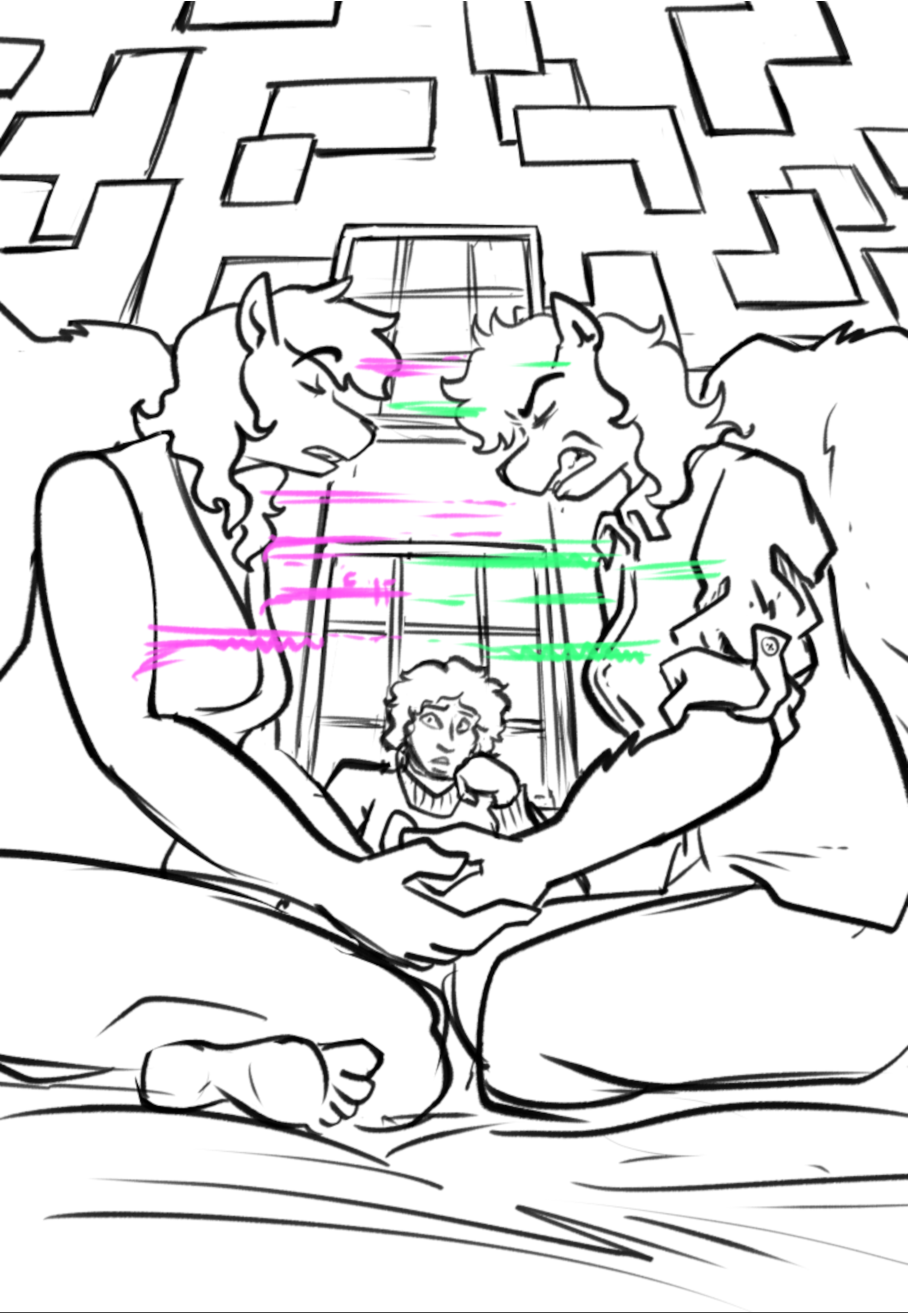
\includepdf[pages={1},noautoscale=true,fitpaper=true]{assets/merge}}

Both Ioan and True Name watched as the down-tree instance of May scrubbed her paws over her face vigorously for a moment, gave a shaky wave, and then quit. True Name winced and screwed her eyes shut, and the May who had knelt with her on the bed reached out and took the skunk's paws in her own.

``Go ahead.''

It was still another ten seconds or so before True Name managed to relax enough to permit the merge to progress, and even then the only visual indication was a slow slump of her shoulders and a relaxing of the muscles of her face.

Ioan stuffed eir hands in eir pockets and did eir best to feel rooted to where ey stood, hoping against hope that ey could keep from pacing. May watched True Name carefully, eyes searching her features for what ey could not tell. She seemed almost frozen, breathing shallowly despite the relaxed set of her features.

And ey stood and watched them both.

The three of them stayed like that for nearly five minutes—two skunks kneeling on the bed while ey watched from beside it—before True Name moved again.

``Oh\ldots oh, I cannot\ldots{}'' she whispered, and started to sag over to one side.

May shushed her quietly and helped her to lay out on her side before settling down with her. They curled together, still facing each other, nearly snout to snout and still holding paws.

Ey stood and watched. Then ey sat on the beanbag and watched. Watched and waited, though ey wasn't sure what for.

It was more than an hour before May forked beside em, took eir hand, and led em from the room. Neither of the skunks on the bed had moved or made a sound other than May asking True Name if she was okay at one point and the other skunk shaking her head.

Once the door was shut behind them, May let out a shaky sigh and padded over to the kitchen. ``That was very hard.''

``Why, do you think?'' ey asked.

She took a moment to pour herself a glass of water before replying. ``I want to be here with you, and I also want to be in there with her, and I also want to go back in time and tell her I do not want to merge, and I also want to go back in time and merge instead of End Waking, and\ldots a-and\ldots{}''

``Come here, May.''

She clutched the water to her chest with both paws, stumbling blindly around the kitchen counter so that ey could guide her to the beanbag.

She sat down and let Ioan rub her back. Only once she could manage a sip or two of water, she said, voice hoarse, ``Did I fuck up, Ioan?''

Ey was still teasing apart the day—or perhaps the last month—but all the same, ey did eir best to respond to what ey suspected lay beneath the surface of the question. ``Do you think she resents you for not just letting her be True Name?''

May whined and set the water glass aside, shifting on the beanbag until she could rest her head on eir thigh. ``I worry that the real reason she wanted to do this was because there is no going back to who she was. One of those `fuck it, burn it all down' situations.''

``There could be some of that, but is that so bad?''

``I do not know,'' she mumbled.

``Can you imagine her being okay staying as True Name and being all cooped up for the rest of eternity?''

She snorted. ``God, no. I think she would lose it.''

``Same, yeah. She'd probably try to pull a Dear or something.''

``And hate every minute of it. You heard her, she likes who she was and all that she did. I cannot imagine her letting that go.''

Ey nodded and combed eir fingers through the fur on the nape of her neck. ``So she'll be left with a complex view of that—or, well, a couple of them, I guess—maybe enough for her to change how she moves through the world. Think it'll be enough for Jonas?''

The skunk rolled until her face was nearly pressed against eir belly to let em pet. ``I do not know,'' she mumbled. ``I do not think even she knows.''

  \hypertarget{ioan-bux103lan-2350}{%
\chapter{Ioan Bălan — 2350}\label{ioan-bux103lan-2350}}

Of all that had happened over the past several weeks, Ioan was surprised to find that it had taken until now for literally anything to feel like it had been planned. Clearly none of them had planned on Jonas coming after True Name, but all of the decisions that had followed had been made on the spot. Snap decisions that had led to True Name moving into their house, to End Waking merging down, to the three of them all overflowing at once.

All of those had been made under what felt like intolerable pressure, and it was only now that they had time enough to relax. There was an uneasy (and certainly temporary) truce between Jonas and True Name that had finally given them enough time to properly consider a decision instead of feeling compelled to make it right away.

Ey'd harbored a concern, one borne out of stress, that May might just merge down without talking further, but ey kept that to emself, doing eir level best to reason emself out of it. The last thing they needed at the moment was eir mind playing tricks on em.

And she certainly didn't. In fact, she drew the negotiations that followed that first discussion out by nearly a week, putting lie to that concern. Much of these discussions took place between the two skunks as they walked out on True Name's prairie.

At first, ey'd felt left out. After all, didn't ey also have boundaries to negotiate and concerns that needed addressing?

After bringing this up with May, however, she had laughed and poked em in the belly, explaining, ``I do not mean to leave you out of anything, my dear. We are discussing elements of the past that kept me from merging down, and elements of the future of the relationship between me and her. You are not missing anything so important, but if you would like, I am happy to keep you apprised of the general content.''

``Given how anxious I've been, I'd appreciate that,'' ey had said. ``But no need to share anything private.''

And so now ey got updates on the conversations with sensitive or personal information held back.

They spent much of their time discussing various parts of May's life and how comfortable she'd feel sharing those through a merge, and if not, why not. Surprisingly, they also talked with End Waking several times, the third skunk of the stanza coming out to visit her prairie so that they could discuss the ramifications of their merge and how to be more thoughtful with May's.

That first meeting had been more silence than not, more walking and thinking and not looking at each other than anything. They paced back and forth along the bank of the river, then stared into the oxbow pond, each occasionally failing to start a conversation. They had greater success with subsequent meetings, but they were never comfortable.

This wasn't to say that ey didn't have a chance to sit with them at times and discuss eir thoughts on the matter, of course.

``Feelings are complex, Ioan,'' True Name explained as they sat around a low fire before her tent. ``If they are created by memories, then there is little that I can do to completely control how I might feel about something beyond picking and choosing the memories carefully. However, one can never be sure which memories may lead to which feelings. If they come from something more intrinsic to one's personality and thought patterns, then it is even more difficult to attempt to control them.''

Ey nodded. ``That much I can certainly understand. I trust that you'll be built up from your various histories rather than simply May's feelings tacked onto you.''

``Yes. I cannot predict how I will feel about anything after this, much less you. Your relationship and existing boundaries will take precedence over whatever happens, though. I will respect that.''

Ioan bowed eir thanks.

``I have been wondering how your feelings toward Debarre have shifted,'' End Waking said.

``It is complex, not least of which because I accepted the whole of your merge so blithely. I will not be doing the same with May Then My Name's.''

He frowned.

``I am sorry,'' True Name said, shrugging helplessly. ``There is little that I could have done in the moment to avoid it, and there is certainly nothing that I can do now to fix it.''

May dipped her muzzle and apologized as well, saying, ``I do feel bad about how that worked out, no matter how much you tell me it is okay.''

``It is not okay,'' End Waking said, then hastened to add when his cocladist flinched away, ``It is what we have to work with, and it is perhaps what the times called for.''

May nodded, still cowed.

``I am of two minds,'' True Name said. ``I remember having loved Debarre. I remember still loving him, and perhaps even I, even True Name, still love him in some roundabout way. However, I am what I am, and that is a being of two minds. That of me which is you, End Waking, loves him, and that of me which is True Name, respects him from a distance, respects his distaste for me, that feeling I engendered to minimize his impact within the council by making it purely emotional, as uncomfortable as it was to do so.''

``The same as you did with me and Codrin?'' Ioan asked. ``With the history, I mean.''

She nodded. ``It was-- it felt like a necessity at the time. I am not some cold, unfeeling bitch, it is just that my drive and my abilities, such as they are, outweigh — or at least outweighed — those feelings. I worked to distance myself from them.''

``I remember so little of that,'' May said.

True Name shrugged. ``As you intentionally moved towards feeling, I worked to contain and compartmentalize it within myself after you came into being. I became a being of negative commandments. I lived the 'shalt not's while you performed your \emph{mitzvot} of loving and caring.''

May sighed.

``I will not say that I am proud of it, my dear, but neither will I say that I regret it. It is what it is specifically because I was what I was.''

``Perhaps you will learn from your merge,'' End Waking said.

``Perhaps. Perhaps it will become a part of me, perhaps it will live within me alongside that of you and that of True Name.''

``Still feeling fractured?'' Ioan asked.

``I am of two minds, Ioan. I do not know if I will feel\ldots{} I do not know. I am not comfortable speaking further on this just yet.''

They spent the rest of the night in quiet, May leaning against eir side while True Name and End Waking spoke quietly about the plain and the forest.

Finally, though, a week to the day after the decision had been made, Ioan awoke to find May and True Name already sitting at the table, speaking earnestly in a cone of silence. Once they noticed em, True Name waved it away and May grinned, saying, ``Sorry, my dear. We did not want to wake you.''

Ey poured emself a cup of coffee before joining them. ``Appreciate it. Hope I'm not interrupting.''

True Name shook her head. ``We are discussing our plan for the day.''

Ey bought emself a moment by taking a sip of coffee. ``Is today the day, then?''

``May Then My Name thinks so, but we were also waiting for you to join us to make sure.''

``Well, if it were solely up to me, I'd just spin my wheels worrying about it until we ran out of time, so I suppose I'm alright with it. What all will go into it?''

``Well,'' True Name began, a fork appearing next to her. ``First I fork and she will head to the tent.''

The new instance of True Name bowed. ``Then the perilous path was planted, And a river and a spring On every cliff and tomb,'' she said before waving goodbye and padding back out through her room.

Ioan stared after the departing skunk and shook eir head. ``You guys are so weird.''

They both laughed.

``Then we will set up a space for me to rest in the meantime,'' True Name continued. ``And then I suppose that is all there is to it. May Then My Name will fork and quit and I will process the merge.''

``And your fork is just there in case something goes wrong?''

``Or if the result is not acceptable.''

``\,`Not acceptable'?''

``If the merge does not go well or if I wind up being unable to work as I would like.''

``Or if all of my emotions get overwhelming,'' May added. ``Since I do rather have a surfeit.''

Ioan leaned over and ruffled a hand over the skunk's ears. ``Yeah, you definitely do.''

``Yes, yes, and you love me for it.'' She laughed and pushed eir hand away, straightening the mussed up fur. ``Breakfast first, though, and then we can work from there.''

After another Scandinavian-style breakfast, the three of them re-organized True Name's room. The bed was set in a corner instead of up against one wall, allowing a collection of pillows to be placed against the walls in case she wanted to lean against them or organize them into a nest.

``Are you sure you don't want to set up something out in the prairie?''

``I did consider it, but May Then My Name talked me out of it, stating that she would like to be at hand without having to spend all of her time out there, herself. Besides, if I learned one thing from End Waking merging down, it was that the less I have to think about my body, the easier it is to focus on my mind. Comfort will only ever help.''

They also supplied her with ready water, juice, and a few comforting snacks on one of the bedside tables so that she wouldn't have to get up just to go to the kitchen.

Another beanbag was added by the bed, in case she requested that they stay in there for any length of time, and a more comfortable bench-swing was added to the balcony in case she needed to go outside but wasn't feeling up to walking down to the prairie itself.

It felt like rather a lot of preparations to make just for a merge, but then May had last merged down 83 years before ey had uploaded — nearly 64 before ey'd even been born — and after seeing how intense End Waking's merge had been, none of them felt up to cutting any corners and having to rush comfort after the fact.

Finally, though, there was nothing left to do, no further preparations to be made that weren't just stalling, so May took eir hand to hold em still so that ey'd quit pacing.

``I don't even know why I'm fretting so much, I'm not even the one merging.''

True Name smiled faintly and shrugged. ``I am fretting too, do not worry.''

``It is a big event,'' May added. ``It will be an even bigger merge and, while it may be more comfortable than End Waking merging down as she has said, it will be no less complex.''

Ey sighed and nodded, squeezing her paw before tugging eir hand free. ``Right. I'll relax and leave you to the rest of it.''

``Please stay, Ioan,'' True Name said quietly.

``Stay?''

``Yes. Please stay. I do not think it will be dramatic, but, well\ldots{}'' She hesitated and frowned. ``You are a grounding person. Is that not what my counterpart on Castor said about Codrin? I appreciate your presence.''

Ey considered any number of responses ey could give before just nodding. If nothing else, ey didn't want to hold either of the skunks up from what would most certainly affect both of them more than it would em.

May forked and the new instance climbed up onto the bed with True Name, the two skunks kneeling, facing each other, amid all the blankets and pillows.

Both Ioan and True Name watched as the down-tree instance of May scrubbed her paws over her face vigorously for a moment, gave a shaky wave, and then quit. True Name winced and screwed her eyes shut, and the May who had knelt with her on the bed reached out and took the skunk's paws in her own.

``Go ahead.''

It was still another ten seconds or so before True Name managed to relax enough to permit the merge to progress, and even then the only visual indication was a slow slump of her shoulders and a relaxing of the muscles of her face.

Ioan stuffed eir hands in eir pockets and did eir best to feel rooted to where ey stood, hoping against hope that ey could keep from pacing. May watched True Name carefully, eyes searching her features for what ey could not tell. She seemed almost frozen, breathing shallowly despite the relaxed set of her features.

And ey stood and watched them both.

The three of them stayed like that for nearly five minutes — two skunks kneeling on the bed while ey watched from beside it — before True Name moved again.

``Oh\ldots oh, I cannot\ldots{}'' she whispered, and started to sag over to one side.

May shushed her quietly and helped her to lay out on her side before settling down with her. They curled together, still facing each other, nearly snout to snout and still holding paws.

Ey stood and watched. Then ey sat on the beanbag and watched. Watched and waited, though for what ey didn't know.

It was more than an hour before May forked beside em, took eir hand, and led em from the room. Neither of the skunks on the bed had moved or made a sound other than May asking True Name if she was okay at one point and the other skunk shaking her head.

Once the door was shut behind them, May let out a shaky sigh and padded over to the kitchen. ``That was very hard.''

``Why, do you think?'' ey asked.

The skunk took a moment to pour herself a glass of water before replying. ``I want to be here with you, and I also want to be in there with her, and I also want to go back in time and tell her I do not want to merge, and I also want to go back in time and merge instead of End Waking, and\ldots a-and\ldots{}''

``Come here, May.''

She clutched the water to her chest with both paws, stumbling blindly around the kitchen counter so that ey could guide her to the beanbag.

She sat down and let Ioan rub her back. Only once she could manage a sip or two of water, she said, voice hoarse, ``Did I fuck up, Ioan?''

Ey was still teasing apart the day — or perhaps the last month — but all the same, ey did eir best to respond to what ey suspected lay beneath the surface of the question. ``Do you think she resents you for not just letting her be True Name?''

May whined and set the water glass aside, shifting on the beanbag until she could rest her head on eir thigh. ``I worry that the real reason she wanted to do this was because there is no going back to who she was. One of those''fuck it, burn it all down'' situations.''

``There could be some of that, but is that so bad?''

``I do not know,'' she mumbled.

``Can you imagine her being okay staying as True Name and being all cooped up for the rest of eternity?''

She snorted. ``God, no. I think she would lose it.''

``Same, yeah. She'd probably try to pull a Dear or something.''

``And hate every minute of it. You heard her, she likes who she was and all that she did. I cannot imagine her letting that go.''

Ey nodded and combed eir fingers through the fur on the nape of her neck. ``So she'll be left with a complex view of that — or, well, a couple of them, I guess — maybe enough for her to change how she moves through the world. Think it'll be enough for Jonas?''

The skunk rolled until her face was nearly pressed against eir belly to let em pet. ``I do not know,'' she mumbled. ``I do not think even she knows.''

  \begin{center}\rule{0.5\linewidth}{0.5pt}\end{center}

Sleep was the first obstacle they ran into.

While True Name had, at one point, sat up long enough to drink half a glass of water, she had yet to leave the bed, and with her still down for the count, the instance of May that had remained was unwilling to leave her side, even for dinner, which she declined.

``You don't think sleeping with her will be enough to keep you comfortable through the night?''

She rolled her eyes and poked em in the stomach with a dull claw. ``It is not just that I do not want to sleep alone. I want to sleep with you.''

Ioan blinked, laughed, and rubbed at the back of eir neck. ``Right, sorry, I guess I've been stuck on logistics mode for a bit.''

``Is this not emotional?''

``It is! I'm just\ldots overwhelmed or something.''

May nodded and looped her arms up around eir shoulders. ``That much I understand, my dear.''

``Would it make sense if I added a cot or something in there? I could at least sleep nearby.''

She perked up and tilted her head. ``One moment. Or\ldots well, come with me.''

May led em to True Name's room where the skunk was slouched over on the bed, head resting in the other instance of May's lap, the two of them tucked into the nest of pillows in the corner.

``Let me reduce--'' The May who had stayed with Ioan quit, leaving the other instance of her to quickly incorporate the merge and continue, ``--conflicts. True Name, are you able to speak?''

The answer was a long time coming. ``Some,'' she croaked.

May nodded. ``I am not going to leave, but it is getting close to bedtime. I am also not comfortable not being near Ioan. May ey sleep in here with us?''

True Name slowly rolled her head to the side enough to squint at Ioan through one eye. Her cheek-fur was a mess of tear tracks. ``Ioan?''

``I can make a cot by the bed,'' ey said, then laughed. ``Or just another, smaller bed, I guess. No need to make one of those uncomfortable things.''

She slowly pushed herself up to a sitting position, though she remained half-slouched against May. ``Can you\ldots make the bed bigger?''

``Well, I mean\ldots{}'' ey shrugged helplessly, looking to May.

The skunk tilted her head back against the wall, looking up to the ceiling thoughtfully. ``I do not see why not, I suppose,'' she said, sounding distant.

``Worried?'' True Name mumbled.

Ioan shifted eir weight uncomfortably from one foot to the other. ``I just, uh,'' ey stammered. ``I don't want to make things weird. I can't even imagine all you're going through.''

True Name laughed hoarsely. ``It is not a comfortable\ldots time for us, no.'' She sighed, sat up further, and rubbed at her face. ``Preference\ldots make bed larger and join\ldots second choice, other bed.''

Ey nodded. ``I can make the bed bigger. Should I make a second set of covers?''

She swallowed several times in a row, a sign of tears to come ey well knew from May. ``Can I ask\ldots can you two\ldots{}''

May got her arms around the skunk and shushed her gently. ``We will work it out.''

Ioan hesitated a moment longer before willing the bed to expand another half meter in width. A second set of covers and pillows spooled themselves out onto it as well, just in case.

Ey paced back and forth a few times, shook eir head, then waved a hand again to bring a set of pajamas into being on the bed. Sleeping in eir usual dress of a pair of boxers didn't seem quite appropriate at the moment.

May blinked down at the clothes, giggled quietly, and shook her head. \emph{``You are such a nerd,''} she subvocalized through a sensorium message so as not to disturb True Name. \emph{``It is a good idea, but you are a total nerd.''}

Ey shrugged helplessly, gathered up the loose lounge pants and shirt to go change.

\emph{``I have no clue how tired I even am,''} ey sent once ey returned. \emph{``Or if I'll even be able to sleep here.''}

\emph{``If you need to sneak off to sleep in our bed, you can.''}

\emph{``I'm} also \emph{unwilling to sleep without you, so\ldots``}

Her expression softened. She tilted her muzzle down to whisper something to True Name, and when she received a nod in response, she signed \emph{okay} and patted the bed to invite em up.

Ey nodded and climbed onto the (now much larger) bed so ey could settle down beside May in the nook of pillows. Getting eir arm around her, ey let her rest her head on eir shoulder. It was a little awkward with True Name still slouched against her side, but it worked well enough.

\emph{``I'm surprised she's so\ldots physical,''} ey sent.

\emph{``She was not, at first, but I suspect she is working her way from past to present. She slowly got closer and closer as she learned how I did the same.''}

It made sense, at least. Whenever ey'd dealt with a longer merge — eir longest had been around thirteen months, and a particularly boring project at that — it always felt like the memories were interleaving themselves in with the ones ey already had, histories slowly zippering themselves into consensus. Conflicts, then, were the snags one encountered along the way, and one would have to dump energy into either reconciling or discarding memories. It was a very consuming task, and that True Name had been able to speak at all was far more than ey could have done.

\emph{``Think it's overriding the bits of her and End Waking that aren't keen on touch?''} ey asked.

\emph{``Must be.''}

\emph{``How are you doing with it?''}

She sighed, at which True Name squinted up to her, then over to Ioan, offering a weak smile before settling back into processing.

\emph{``I do not know, my dear. It has activated all of my care instincts, so I am happy to make her comfortable in all of the ways I know how. It helps, then, that those are all of the ways she knows now, too, or at least is learning. If I focus on that, I feel very positive. It is only when I get distracted and ruminating that I begin to spiral. It is more comfortable for me to focus on caring for someone now than it is to think about boundaries or Zacharias or Jonas.''}

Ey kissed between May's ears, murmuring, ``You're a good person, May.''

The skunk lifted her snout to tuck it up under eir chin.

``You two\ldots are disgusting,'' True Name mumbled. ``Keep it up.''

May laughed and tightened her grip around her briefly. ``Hush, you. We will work on going to bed soon. I hope that you can get some sleep.''

She only shrugged.

``Well, either way, I will let you keep the corner nest and be right here. Ioan can take the outside.''

``Keeping em\ldots away?''

May frowned. ``I am keeping myself close to you.''

``I kid. I have not\ldots even gotten there, yet,'' True Name said, slowly pushing herself up once more and frowning at just how far away the glass of water was. Ioan leaned forward to grab it for her. She drank carefully. ``But if it\ldots also keeps awkwardness down\ldots that is good, too.''

Ioan accepted the glass from her once she finished, re-filling it from the pitcher they'd brought in and setting it on the windowsill near the nook so that she could get to it herself. ``We can talk about that later. For now, I think it'll work alright.''

True Name nodded and settled down into her nest of pillows.

May and Ioan stayed up a little longer, chatting through sensorium messages to let True Name process in peace. Cognizant of her mention that she felt better when not thinking about boundaries, ey kept the topics light, asking about favorite things and letting her rant about plays from her past that she'd hated.

Nearly an hour later, just as May started to nod off, True Name yelped and sat up, scrambling back against the wall away from them. ``You know!'' she shouted. ``Codrin knows!''

It took only a moment for understanding to click into place. Both ey and May sat up to give her a bit more space.

``Hush, my dear,'' May said, voice soothing. ``It is okay. Remember Dear's letter.''

``I\ldots I cannot-- It is too much!''

Ioan held still, hands flat on eir thighs. The urge to wipe the sweat from eir palms was pressing against em, but ey wanted to at least appear calm, even if ey didn't feel such.

May began to crawl towards True Name, then stopped when her cocladist shied away from her. ``Codrin has not spoken it aloud, not even with True Name\#Castor. I confirmed with Dear: ey only said \emph{that} ey heard it, and that is all that ey told Ioan.''

She snatched a pillow from the pile and clutched it to her chest, wide-eyed. ``Why?''

``Ey couldn't be the only one,'' Ioan said quietly. ``We don't do as well under pressure as you, we don't\ldots well\ldots{}''

``Keep secrets?'' she growled.

May held up her paws disarmingly. ``They keep secrets very well. They just do not keep many.''

She glanced sharply at May, then said to Ioan, ``Ey did not tell you the Name? No one else knows?''

``No.~The message was individual-eyes-only. I haven't even shown May.'' After a moment's thought, ey added, ``But I can unlock it for you, if you want. It's in an exo I haven't looked at since.''

``Sweep the whole sim,'' she snapped.

Ey nodded, swept the sim of everyone but the three of them, and instructed the perisystem architecture to print out the \emph{0 individuals swept} receipt onto a slip of foolscap, which ey handed over.

``Move back, May Then My Name,'' she instructed, quieter this time. When May obliged, the skunk crawled closer to em and set up a cone of silence with secure visual ACLs. She was panting and shaking, though ey was pleased to see that at least the anger that had swelled briefly had subsided once more into something more manageable. Ey didn't think any of them were up for a shouting match. Once she'd knelt beside em, whispered, ``Show me.''

Ey drew the sheet out of the air, holding it up for True Name to see the fully redacted text, then unlocked it for her eyes only and handed it over.

She read it through top to bottom a few times, set it down and kneaded her paws against her face, then picked it up to read it once more.

Finally, shoulders sagging, she handed it back. ``Re-secure it and destroy it, please.''

Ey did so and held up eir hands. ``I'm sorry, True--''

She patted eir arm with a shaking paw. ``Please do not apologize.'' After dropping the cone of silence, she continued, ``I should have\ldots I should have learned from\ldots I am sorry.''

May held out a paw once more, and this time True Name took it, letting herself be guided back to the nest of pillows, where she slumped down once more, expression glassy. ``Could themself have peeped — And seen my Brain — go round —'' she mumbled.

``Rest, my dear. It is okay,'' May said quietly. ``Do you want company?''

``Too much\ldots but I\ldots{}'' After a shuddering breath, she shook her head. ``I will\ldots be fine. We will speak later.''

May nodded and crawled back over to Ioan, nudging em to lay down so that she could tuck in against eir front. She remained tense, and when ey sent a gentle sensorium ping, she sniffled and shook her head.

Tiredness eventually won them over, though, and, despite the room being mirrored from what ey was used to, the bed was the same, comfortable one ey'd slept in for the last century, the house held the same sense of `home' as ever. May curled against eir front as she always did, and while it was strange seeing True Name just beyond her, it was still where ey belonged.

The last thing ey remembered before falling asleep was watching the way True Name had curled to face May, the two skunks holding each others' paws once more, and thinking to emself, \emph{This isn't how I pictured things winding up if I had somehow been able to fix things between them, but it could certainly be worse.}

\begin{center}\rule{0.5\linewidth}{0.5pt}\end{center}

Waking brought confusion. Something about the inversion from their normal bed, of having fallen asleep on eir other side than ey usually did, induced a subtle sense of vertigo at first. The pajamas were also bunched up around em strangely, adding a subtle sense of constriction. As sleep slowly seeped away, though, the feeling lessened and ey was able to relax in the warmth beneath the covers.

Warmer than expected, perhaps. May was still in eir arms, as usual, but the position felt off with the addition of a second warm bulk.

Ey tried to puzzle it out through the fog of doziness that still surrounded em. Eventually, ey gave up and levered eir eyes open, blinking a few times to bring the world into focus.

At some point in the night, True Name had apparently rolled over and wound up curled in May's arms, much as she was curled in eirs, and with with eir arm resting atop May's, ey was left hugging two skunks.

Ey lay there for a while, groggily trying to piece together eir thoughts on the situation. As far as ey could remember in eir still sleep-addled state, ey'd never been this close to True Name before. There had been the occasional casual touch, a few touches out of necessity — grabbing her hand to get away from Guōweī, lifting her after End Waking's merge — but even going back to when ey'd first met her, there'd been very little touch. It made sense, given her personality, and yet here she was, all cuddled up with the two of them. If nothing else, ey should probably decide whether or not to extricate eir arm from the situation to ease that awkwardness.

Ah well, ey was probably worrying too much about this, just laying there and ruminating.

\emph{``You almost certainly are, Mx. Bălan,''} came the barest whisper of a sensorium message. \emph{``Especially if you are mumbling.''}

Ey jolted at the words impinging on eir senses, getting a sleepy grumble out of May.

\emph{``Sorry,''} ey replied to True Name.

There was a note of amusement, of almost-laughter, as she sent, \emph{``It is okay, dear. What are you worried about? You only mumbled the last bit.''}

Eir mind raced as ey tried to figure out how best to explain what ey'd been cycling over.

\emph{``I rolled over sometime in the night — I do not know when, I was memory-sick — and have been staying still to keep from waking you two. Would you like me to move?''}

\emph{``No\ldots{}''} ey replied hesitantly. \emph{``But you guessed right. I hope this isn't weird or anything. If you need to--''}

\emph{``Ioan, I asked after your preferences,''} she chided. \emph{``I am okay, I promise.''}

Ey hid the heat rising to eir cheeks by burying eir face in May's fur. \emph{``Right, sorry. You're okay there. I'm just being awkward.''}

Ey felt True Name relax. \emph{``We both are. It is comforting and awkward in equal measure. One third of me is very happy to be held, one third would really rather not be touched, and one third is simply confused. I am of three minds.''}

\emph{``Have you finished merging, then?''}

There was a subtle rustle of fur against pillow as the skunk shook her head. \emph{``I have the memories in place, but there are many conflicts yet to process. It is easier to put those on hold, at least, so that I can make fun of you for mumbling for a little bit.''}

Ey smirked. \emph{``Har har. All the same, I'm glad you made it through to this far, at least.''}

\emph{``Thank you, Ioan. As am I.''}

They fell back into silence then. Ioan spent a while marveling at the mix of coziness and strangeness. It \emph{was} comfortable, there with the two skunks. May was in eir arms as she should be, and True Name, similar as she was, fit well enough in the mix. The strangeness, then, came from the knowledge that she was specifically True Name. This was so counter to what ey knew of her from the years prior, especially the version of her that she'd become over the past few weeks since End Waking's merge.

Ey could already tell that she'd changed, though, even beyond the fact that she'd wound up as close as this. Her speech patterns were shifting once again, losing some of their formality, finding their way back to ground from the high-minded patterns she'd picked up from her other cocladist, and yet they weren't totally those of May, either. They didn't sound the same, just more alike than they had before.

She was tripled, now. She was True Name and she was End Waking and she was May. Whether or not she would become something new or remain thus ey didn't think even she knew. The adjustment would certainly take time for everyone. Ey liked End Waking quite a bit as a friend, but that friendship was different than that of eirs with True Name. Ey was friends with May, but in that way that partners were still friends beneath the romance of a big-R Relationship, and there was certainly no comparison to be made between the other small-r relationships. If she was of three minds, so was ey.

\emph{``Unrelated to comfort or awkwardness, I am going to get up to make coffee,''} she sent, nudging em out of rumination once more. \emph{``I did not sleep, and if I do not have coffee soon, I shall surely die.''}

May grumbled again when True Name rolled away from her, gathering the remainder of the covers and a stray pillow up to replace the space that had been left by her cocladist's absence. Ey couldn't tell if the skunk was actually awake or not, but she settled down once more, if nothing else.

True Name sat up and scrubbed at her face with her paws, wiping the grit of sleep — or perhaps tears — from her eyes. She grinned down to em. \emph{``My assessment remains. You two are so cute that it is disgusting.''}

Stifling a laugh, ey rolled eir eyes. \emph{``Blame May.''}

\emph{``Way ahead of you, dear,''} she sent as she crawled out of bed. \emph{``I will make coffee and then I will need some alone time on the plain. I will ensure there is enough for all.''}

There was a quiet clattering from the kitchen, mugs being shifted about and the coffee pot being set in place, doubtless another instance of her making enough noise to let them know what she was up to.

It was enough to wake May the rest of the way, the skunk stretching out against eir front and yawning wide before she shifted about to face em. ``Pillows,'' she mumbled, peeking down at the bundle she still held in her arms. ``Oh, did I\ldots?''

Ioan nodded, placing a kiss atop her head. ``She said she rolled over against you, yeah.''

``Sorry, Ioan.''

``It's fine by me, I slept through most of it,'' ey said, chuckling. ``She and I talked about it a bit before you woke up. She's confused about it, but seemed like she needed it.''

``She is learning my wicked ways,'' she mumbled against eir front. ``I am happy to hear that it was helpful and that you are okay with it, though.''

``Mmhm. How about you?''

May yawned again before poking her nose up against eir chin. ``I do not know. I slept through it, too, apparently. It fits with what I said earlier, though. I am pleased to care for those around me.''

``She also called us disgusting again.''

``That is because we are. Is that her making coffee?''

Ey nodded, nudging her snout with eir chin.

``Good girl.''

A few minutes later, True Name returned, carrying three mugs of coffee. Ioan and May pushed themselves up to sitting so that they could accept.

``I am sorry I shouted last night. I think I understand Dear's letter better now.''

May nodded.

``I was wondering if you didn't know about\ldots all that before last night, honestly,'' Ioan said.

``I have been fed bad and incomplete information for years now. I had not suspected just to what extent. I am still frightened, if I am honest, but I will trust you two on this. It is complicated and bound up in emotions I do not understand, but I will trust you.'' She shook her head. ``But I cannot speak of it any more right now.''

``Heading outside?'' ey asked.

She nodded. ``Yes. I will need an hour or so of nothing but the morning and the grass.''

``Of course.''

May nodded. ``Take the space you need.''

True Name leaned over enough to dot her nose against the skunk's cheek. ``Thank you, dear. If you cook breakfast, I will refrain from telling Ioan embarrassing stories.''

``Asshole.'' She laughed. ``Where did this humor come from?''

``Your guess is as good as mine, at this point.''

``She seems to be doing well,'' ey said, once she'd made her way outside and down the stairs to the prairie.

``It helps that I did not drop a merge onto her unexpectedly. She had more to process, but more preparation to do so.''

``She said she's done getting the memories in order but working on conflicts now.''

May nodded. ``About a third of the way done, then.''

``It's really gratifying to see it going so much more smoothly this time.''

``Agreed, yes,'' she said between sips. ``I was not expecting her to turn into a cuddlebug, but I suppose that will level out before long. Was that awkward, this morning?''

Ey shrugged. ``A little, I guess. Just hard making it work in my head. Doesn't fit with what I remember of her.''

``I cannot picture you getting cozy with \emph{just} True Name, no. I can barely picture her getting cozy with anyone, and that is certainly not even bringing End Waking's general touch-aversion into the equation.''

``I'd assume she got cozy with Zacharias, if they were together.''

May's expression soured. ``We will need to talk about him soon, but I cannot talk about him now.''

``Of course.''

She made a setting aside gesture, stepping back to the previous topic. ``Did that feel like crossing a boundary?''

``Not particularly, no. It just felt like me being awkward, more than anything.''

``That is good, then.'' She finished her coffee and waved the mug away. ``I do not know how to feel about it, myself, because I do not know what she will be like when she has finished incorporating the merge. She is not yet settled enough, so I will forgive much that I might not otherwise.''

``It's not like she was hitting on me or anything,'' ey said, laughing.

She smirked. ``Are you sure?''

Ey reached over to tug on one of her ears gently. ``Yes, I'm sure. I'm dense, but not \emph{that} dense.''

The skunk tilted her head at the tug, laughing. ``Has your opinion of her as a friend changed?''

Ioan tilted eir head. ``How do you mean?''

``I do not imagine that you felt the same about her when she was just True Name as you do now about who she has become. Or is becoming, at least.''

``Well, no,'' ey hazarded. ``But I don't know just how, yet.''

``Me either.''

They reconvened over a simple breakfast of scrambled eggs and bacon with toast.

``I instructed my fork to quit,'' True Name said by way of opening the conversation.

``Feeling positive about the merge, then?'' ey asked.

``Yes. Having worked through some conflicts, it will not be easy, but I am comfortable with the direction in which it is going.'' She took a bite of toast piled high with eggs and a small piece of bacon, chewing thoughtfully. ``It is not all positive, but it has given me hope for a pleasant life moving forward.''

``Was your life unpleasant before?'' When May frowned at em, ey held up eir hands. ``Sorry, maybe that's impertinent. It's not important.''

True Name shook her head. ``It is okay. It was, yes. It was fulfilling. I felt hopeful and comfortable with the path I had chosen. The work itself was starting to grate on me, but that had less to do with the work than the coworker. Pleasantness was never a focus for me, however.''

May, having subsided, finished her bite of toast before asking, ``Did you have hope for happiness with just End Waking's merge?''

``No.~Not at all.'' She reached out a paw to give one of May's a squeeze, adding quickly, ``Again, I understand — now more than ever — why you did what you did, and I do approve of it in light of what is happening with Jonas, but it was an uncomfortable duality in comparison to this more comfortable plurality and I may yet settle into a new singularity. I do not know.''

May smiled gratefully, returning that squeeze.

``Meeting up with my fork hammered that point home pretty well. She looked\ldots well, I will not elaborate on the differences I saw. Seeing myself through her eyes, I can tell that she was pleased as well.''

``I am very happy to hear that,'' May said. ``Not least of which because you seem to be building a new self rather than simply a raw combination of us.''

True Name nodded, finished her plate before setting it aside. ``Thank you for breakfast, May Then My Name. Your secrets are safe for another day-- ow!''

``Your high station does not preclude you from being kicked, my dear,'' May said sweetly. ``You deserved that.''

The skunk preened.

Ioan watched the exchange, grinning. Beyond just what she'd said, ey could read relief in May's features. That resentment towards her down-tree instance had never quite gone away, ey knew, and, on some level, it likely never would. Still, that True Name was, as the skunks had said, rebuilding herself into a new person seemed to have brought out a new sense of friendliness within eir partner that had been lacking to that point.

Ey wondered if she would go through a reevaluation of who True Name had been before, much as ey had. It was certainly enough that she felt more positive, but ey — em and Codrin\#Castor, perhaps — seemed to have dropped much of that resentment that had lingered in May and so many others, though whether that was due to a difference in temperament or the relatively short time they'd known the skunk in comparison, ey couldn't tell.

``Is it just me, or is eir mumbling getting worse?'' True Name stage-whispered to May.

She whispered back, ``Perhaps the centuries are catching up to em. Is this how the Bălans crack? Should we warn Dear?''

``Are all skunks such pests?'' Ey smirked.

They laughed.

``I mumble more when I'm stressed, that's all.''

``Are you stressed now, my dear?'' May asked.

``It's a stressful time overall, even if this particular morning is pleasant enough.''

``It feels rather like the morning after a sleepover, yes,'' True Name said.

May nodded eagerly.

``I've never had one of those, so I'll have to take your word for it. Do those always come with cuddling up in the morning?''

Both skunks splayed their ears and dipped their snouts.

``It depends on the sleepover,'' May said, adding to True Name, ``Are you feeling well enough to discuss boundaries now?''

She hesitated. ``We can begin the conversation, though I will need to address further conflicts before long.''

``To be clear,'' Ioan said. ``I'm okay with it, it was just unexpected.''

True Name gave a hint of a bow. ``One thing that came up in our discussions leading up to the merge is that the one with the greater restrictions in a relationship defines the boundaries. Right now, I suspect that may be one of you two. I am the outsider, here. I have never had to have a conversation such as this.''

``My comment about you building up a new self has gone a long way towards soothing any fears,'' May said. ``I think I was worried you might incorporate my memories of the last few decades wholesale and wind up feeling exactly the way that I do about Ioan.''

True Name shook her head. ``I have taken to heart your requests and declined the personal memories you suggested. There are many conflicts,'' she said, speaking more slowly. ``Perhaps due to your feelings about me as I was, so I am not sure how I feel yet, but\ldots well, may I speak earnestly?''

May and Ioan both nodded.

``On that point, I remember enough to know why it is that you love Ioan. I can see what it is that you see in em. It is as if\ldots{}'' She trailed off, ears pinned flat. ``This is so fucking embarrassing. I am sorry. Uh\ldots it is as though there is a world in which I could do the same, but I do not know how to get from here to there. Again, I am sorry, May Then My Name.''

There was a long silence around the table while Ioan and May digested this. True Name spent it resting her head in her paws and staring down at her plate.

It was May who broke the silence, saying simply, ``May.''

True Name sniffled and lifted her head. ``Sorry?''

``Stop calling me May Then My Name.''

``I--''

``Do not make it weird, True Name,'' May said, laughing. She held out a paw toward the skunk ``Just fucking call me May already.''

``Right. May,'' True Name said, gingerly resting her paw in her up-tree instance's.

``I do not know how you get from this world to that one, either, should that even be something you want, but,'' she said, taking a deep breath, ``so long as you come by that path earnestly and we discuss it in the moment, it is your path to take. Do you have any thoughts, Ioan?''

Ey held up eir hands. ``Don't look at me. I don't have a clue.''

They laughed.

``We'll see, I guess,'' ey said, shrugging. ``It's all way too much for me to take in right now.''

``Perhaps that is a good place to pause,'' True Name said. ``This conversation has those conflicts begging for attention.''

``Of course, my dear,'' May said, giving her paw a squeeze. ``Go and walk. There will be time for discussions to come, especially once we are finished with this unpleasant political business.''

  \hypertarget{debarre-2350}{%
\chapter{Debarre — 2350}\label{debarre-2350}}

When Debarre received the ping from End Waking, he quickly excused himself from dinner and dashed out into the back yard to respond. The last time he'd received a message in the middle of a period of overflowing, it had been when the skunk's leg had been impaled on a branch, so he hoped against hope that it wasn't the entire tent washing away in a flood this time. It was getting on in spring — still a bit early for floods, but one never knew\ldots{}

``E.W.?'' he said. ``What's up? You okay? Is the tent?''

``The tent is fine, my dear,'' he replied. ``I apologize if I interrupted, but I have some news regarding May Then My Name, Ioan, and True Name, and you requested that I message you. Besides, I need to speak about it with someone other than them. Someone not an Odist.''

He frowned down to the lawn, kicking at a tuft of crabgrass. ``Well, if you're getting in touch, I'm assuming it's urgent.''

There was a sense of a sigh from the other end. ``I am sorry, Debarre.''

``Fuck, I'm sorry, E.W. That came out way snarkier than intended. I understand. I only meant to ask if it was the type of thing where I should fork and come by right away.''

``Please,'' End Waking said, sounding relieved. ``There is nothing to be done, but I am very impatient to speak with someone.''

``You? Impatient?'' Debarre laughed. ``I'll be right over.''

He forked off Debarre\#RelEW and watched him step from the sim, then spent another few seconds looking out into the yard, trying to remember the last time anything had been so important that it had required him leaving immediately. Something other than a tree falling on his boyfriend, that is.

``Well, shit,'' he muttered, turning to head back inside. ``This is gonna be a mess.''

\begin{center}\rule{0.5\linewidth}{0.5pt}\end{center}

Debarre\#RelEW was greeted by the sight of End Waking kneeling in the clearing across from May Then My Name.

``Oh, company,'' he said, frowning. ``Wasn't expecting two of you.''

``You messaged\ldots wait, does that mean you are a fork?'' May Then My Name said, frowning at End Waking.

``It does, yes.''

``I never knew you had it in you,'' she said, sounding proud. To Debarre, she said, ``Did this asshole tell you why I am here?''

He gave her a hug before sitting down with them. ``He said it had something to do with you, Ioan, and True Name, and that he needed to talk to a non-Odist. That's why I was surprised.''

She grinned. ``You will have your chance, my dear. I will not be here long. I needed to step out for a moment, and figured I would catch End Waking up. I am happy to see you as well, though.''

``Happy to see you too. You're always welcome over to my place, too.''

``Of course, yes. This did involve End Waking, though, so alas, I could not go make you uncomfortable with my flirting.''

He shoved at the skunk, who giggled.

``Well, okay. What's up? You finally merge down?''

She blinked, looking startled. ``Yes, actually. How did you guess?''

``Ioan mentioned it when we talked last. How'd it go? Did she explode?''

``Not at all, no. Actually\ldots{}'' She shrugged, poking at the dirt with a twig. ``Actually, I am finding myself rather fond of her, now.''

``Bullshit,'' he growled.

``Debarre,'' End Waking murmured.

May Then My Name waved a paw. ``It is okay. You do not have to like her. You do not even have to interact with her. End Waking wanted you to know about some of the practical considerations, but neither of us are planning on swaying your opinion of her.''

He frowned and leaned back on his palms. ``Sorry. I guess I'm just worried about you. She's not exactly known for her openness and honesty without ulterior motives, so.''

She smiled wanly. ``No, she is not. A fact I have not forgotten. Needless to say, I merged down, and she is making plans to meet up with Jonas, now.''

``That falls more in line with practical concerns,'' he conceded. ``And Jonas still wants both of you there?''

``As far as I know, yes,'' End Waking said. ``I have spoken with True Name several times over the last few weeks and she has a plan of sorts. I do not know how successful it will be, but it is better than nothing.''

``Wait, \emph{you've} been talking with her, too?''

``Yes.''

He shook his head. He could already feel his hackles up, and this wasn't helping. ``Can't fucking believe it.''

May Then My Name frowned, leaned over to hug him around the shoulders, and whispered, ``I am going to leave you to it, but first, remember who you were, who you are, and imagine who you will become. Let go, have fun, but above all, remember that you love him and that he loves you. Those are the rules of engagement.''

After a moment's hesitation, he returned the hug. Had she said it in anything less than her most earnest voice, he might have scoffed, but as it was, he could see himself falling for the gentle manipulation as though from a meter above. He could resent her, but she had said exactly what it was that he needed to hear.

Because of course she had. She was May Then My Name Die With Me. She knew just how to. She was built to.

``You're such an asshole,'' he whispered back, then kissed her cheek to take any sting out of the words. ``I'll do my best. Now, shoo.''

She laughed and licked at one of his whiskerpads. ``Yes, yes.''

After she leaned over to pat End Waking on the knee, she stood up and stepped out of the sim.

Debarre rubbed his paws over his face. ``Where's your root instance? Within an hour's walk?''

End Waking nodded. ``Up-river, yes. Would you like me to walk you there?''

He shook his head. ``Give me some time to think. There's still some of me that's stuck on dinner parties, then another chunk on this whole thing, and another still on May telling me about these rules of engagement or whatever.''

The skunk smiled faintly. ``Twenty minutes' walk up-river, then. He will know that you are coming.''

After End Waking quit, Debarre started to trudge up the faint trail that they'd already worn heading up along the river.

He knew that May Then My Name was right, that he probably needed to at least take into account that if Sasha and Michelle could change enough to make the Odists, then surely True Name could change enough to become someone that even her up-tree instances could like, just as he knew that he probably shouldn't take that out on his boyfriend, frustrated as he was.

Still, it was hard to square the image of End Waking and True Name meeting up voluntarily. What was it that he'd said when Ioan had come by asking after camping supplies? \emph{``I will help but I will not speak with her''}?

\emph{Remember that you love him,} he thought, even as he trudged up the path. \emph{Even if you're working to undermine all that shit that she's done with Jonas, at least you still love E.W.}

The skunk was crouching at the edge of the stream, washing his paws after having apparently just finished gutting a trio of large trout.

``I understand if you are upset, Debarre,'' he said, keeping his gaze on his paws as he scrubbed rather than looking up to him.

``No,'' Debarre said, sitting down next to him. ``Or, well, I am, but it's whatever. I just don't see how something as stupid as May Then My Name merging down solves anything about this. Suddenly, you two are all buddy-buddy?''

End Waking shook his paws free of most of the water before drying them on the hem of his cloak. ``We are not. I am pleased that she is no longer who she was, but she is not a friend. She is not me.''

``But you're visiting her!''

``On business, such as it is. May Then My Name has asked me over a few times.'' The skunk finally looked at him, gaze level and expression flat. ``Did you not say that you would rather she not die?''

``Yeah, but that doesn't mean that you need to interact with her. I don't want her to get offed by some asshole politician, but I also don't particularly want her in my life.''

End Waking shifted from his crouch to sitting cross-legged on a rock on the bank of the river. ``I do understand that, yes. I do not particularly want her in mine, either, but I am now a part of hers, whether she likes it or not. I have been able to help her process some aspects of the merge and also tell her more of how I feel to her face. Once this is over, she will not need to be a part of my life any more if I so desire, and I can move on to defining myself through something other than penance.''

Debarre scratched a claw through the dirt of the bank, worrying a pebble free so that he could throw it into the river while he thought. Finally, he nodded, saying, ``Okay, I get that. What will you define yourself as, then? Like, don't get me wrong, I'm happy you aren't her, and in part specifically \emph{because} you aren't her, but that's not the only reason I love you.''

``I do not know, my love,'' he said after a long silence. ``If I am defined by not being her, by not being what I was, then what is left? I cannot say my love for you, because all of the clade has that to some extent. I cannot even say that I have being an Odist, because, after all these years and with all of her changes over the last few months, I am not even sure that I am that.''

``You can be just End Waking,'' Debarre said gently. ``Like, you can just drop the clade and be that nerd who lives in the woods.''

The skunk laughed and elbowed him in the side. ``We have rather turned our clade identity into idolatry of a sort, have we not?''

``Don't get me wrong, I like where you came from, but I won't be pissed if you drop your clade signifier. Hell, maybe you can even start saying things like `don't' and `isn't'.''

``Do not push your luck.''

They laughed.

``You don't have to have this sorted out, though.'' He shrugged, adding, ``You don't even have to stop seeing True Name. I'm sorry I got angry there. I think I just got upset because any chance that you might start liking her felt like something of a betrayal.''

``I am a ways off yet from liking her, Debarre. I will not say never, but I have gotten to the point where I tolerate her. I will not betray you, though. You or your reactionary friends or whatever she called them.''

Debarre scrambled to his feet, eyes darting around through the trees. ``What the fuck?''

``The sim is empty, my dear,'' the skunk said calmly. ``I empty it every time someone enters.''

``Yeah, but--''

``I think about you a lot, Debarre. Certainly more than anyone else I think about. I have pieced together enough.''

He growled. ``Well, shit. I mean, I guess I'm an obvious enough choice for it.''

``You are, yes, and doubtless the powers that be have been keeping their eye on you since the dissolution of the Council. I do not know the specifics, nor do I want to. As I said, I will not betray you.'' End Waking smiled wryly, adding, ``And I do not think I am of much interest to any of them, anyway. I rarely leave, and I never enter a building when I do. I am more focused on my next meal than anything else.''

``Skunks just wanna get fat.''

End Waking grinned toothily. ``It is not \emph{not} true.''

``Well, anyway. Fair enough. I don't imagine you'll be ratting us out, and you're right that they probably already know. I'm just glad that you've been sweeping the place.''

``I have never caught anyone hitchhiking on you, though I have on May Then My Name and Ioan.'' He shrugged, gathered up the line of fish. ``But speaking of fat, can we go back to cook these? I am not ready for you to stay over, but I would like to eat dinner with you, if you are up for it.''

  Debarre was still mostly full from dinner at home, but he had a few bites of fish forked from End Waking's plate. Tasty, but, as always, lacking in salt.

After they ate, End Waking tasked Debarre with washing off the plate while he tucked another small log into the stove and started the kettle for tea, which they shared while sitting on the step at the entrance to the tent, keeping the last of the spring chill away.

``So, my political junkie friends aside, do you have a better idea of what's going on with Jonas and company?''

End Waking shrugged. ``A little, perhaps. I think it is this upcoming audio-video tech. I do not think he wanted--''

``Moment,'' Debarre said, holding up a paw while he sent a hasty message back home. ``Sorry. We'd been guessing at that, just sent a confirmation. Done now.''

``Please do not act on it yet, my dear.''

So serious was the skunk's tone that Debarre set down his mug and turned to face him. ``I won't, but you gotta tell me why.''

``I am going to be at this meeting. I should probably not even know about their AVEC, but I do because of True Name.''

``And given you and I, there's probably only one place I'd get it,'' he guessed and, when the skunk nodded, sent another message back home. ``You sure this place is secure, then? And you're sending a fork, right?''

``Yes and yes.''

``Good.''

End Waking smiled. ``I know that you do, but it is always pleasing to have confirmation that you think so much of me, Debarre.''

``Of course I do,'' he scoffed. ``But I interrupted, sorry. You were saying?''

``Right. With this AVEC technology, I think that Jonas sees an opening to edge True Name out. I do not know why, but she mentioned something about a diversity of governance across Systems. I do not agree with him on this. I think he is playing a dangerous game by treating each of the Systems so differently. Each System treating itself as a separate country is one thing, but potentially destabilizing them by forcing upon each a different form of governance feels like him treating politics as his personal plaything. I do not like it.''

The longer End Waking spoke, the deeper Debarre's frown got. ``Yeah, ever since they set up that Guiding Council thing over on Pollux, we've been wondering about that. It sounds innocuous enough. Reasonably close to the Council of Ten over on Artemis, I guess, just folks you can go talk to about disagreements and mediation, at least on the surface. That part was inoffensive, but that they would even do such a thing in the face of the \emph{History} is just wild.''

End Waking shrugged. ``You know more than I on that end. I do not keep up with either LV beyond what you and Ioan care to pass on. There are messages from the clade, but you know my feelings on them.''

``Mmhm.'' Debarre hesitated, then added, ``Though if you do wind up going through them and come across any juicy details about those politics you don't care about, you could always share them with me.''

He laughed and shook his head. ``Should my life become so boring, you will have more to worry about, my love. I am better at being a pest than you give me credit for.''

``Fine, fine. I'll just get them from May Then My Name.''

``You will have to put up with her ceaseless flirting.''

Debarre grinned. ``I'm pretty well used to it by now. You're really going to go to this thing, though?''

End Waking nodded, chewing on a mouthful of tisane-bits. ``Yes.''

``Why, though? Isn't that gonna be dangerous? Never mind totally outside your interest. It'll all be politics.''

The skunk was a long time in answering, staring out into the forest and listening to the far-away rush of the waterfall. ``There is what Jonas hopes to accomplish and what I hope to learn. Jonas, I think, would like to gloat. He would like it known that he can loop even me into his plans. He would like even me, even the recluse, scared so that he may use me as a lever over True Name if she is to come out of this alive.''

``And me.''

``And you, yes. I do not doubt that even he knows what you are up to these days, though I do not know to what extent.'' He poked around in his mug to hunt down the last of the gooseberries. ``I am pleased that you are so careful. I worry about you.''

Debarre sat, silent. The comment all but demanded silence from him, so rare was any expression of worry from his boyfriend.

``I will be going because if this is to be the end of True Name then it will be a step towards letting go. It will be an in for me to become independent. If I am to move beyond that which defines me, I would like to know how.''

``Still thinking of cutting your ties? Dropping the clade name?''

End Waking shrugged. ``Would that be so bad? May Then My Name would become simply a friend, rather than a cocladist. True Name would become someone I know rather than a down-tree instance. I do not speak with the others. Serene, perhaps? But even then, it has been many years. It would not change my relationship with you. The forest will not care if I am an Odist or if I am not. To it, I am called Nobody, and when I die and moulder beneath the roots, then it will say that it feasts on Nobody.''

Debarre sighed. Hearing End Waking talk so much was a rarity, but that the death-thoughts were still there meant it'd be a while yet before he'd be allowed back to stay.

``And AwDae? The Name?'' he asked. As he always did when Debarre said their friend's name, the skunk stiffened, hunched his shoulders, and drew his hood up over his head. All the same, he'd made it a point to say it at least once per visit. There had been a row the first few times, but he'd won on the point that AwDae had been his friend, too.

``I do not know, Debarre. That is, I think, the one thing that I will ever defer to True Name on.''

He snorted. ``Really?''

``If she, of all of us, were ever to feel comfortable speaking it, talking about em, then I will know that this embargo will have been lifted.''

``Well, fair,'' the weasel said, finishing his tea before handing the mug back to End Waking to let the skunk snack on the remnants. He'd never really enjoyed them enough to do so himself. ``I'm happy for you, you know that?''

He laughed, swallowing the spent lemon balm and mint he'd been chewing. ``Happy?''

``Yeah. Like\ldots{}'' Debarre trailed off, hunting for words. ``I've never seen you move forward so much all at once. Or at all, really. Like, it's not a bad thing to have a life that you're happy with, but watching you work on the things you \emph{weren't} happy with is nice to see. Kinda glad May Then My Name talked you into the merge, honestly.''

``It has brought me a lightness, yes. She is meddlesome, but kind-hearted.''

``You're telling me. She gave me rules of engagement when I first showed up. Thought she was being weird, but they worked pretty well.''

``She is a brat.''

Debarre laughed. ``You all are. But hey, I should get going.''

The slight sag in End Waking's shoulders spoke of relief. He nodded, saying, ``Of course. Thank you for the chance to talk.''

``You'll let me know when you're going out to this meeting, right?''

``Of course.''

``And you promise you'll send a fork?''

``I will.''

``And call if you need?''

``Debarre, shut up,'' End Waking said, patting his knee. ``Go. I will keep you up to date.''

``Fine, fine.'' He gave the skunk's paw a squeeze and grinned. ``Love you.''

``Love you too.''

Debarre quit, rather than bothering with stepping back home. The pile of experiences caught his down-tree instance in the middle of a sentence — thankfully something unimportant — and he had to spend a minute reconciling the memories with the ones he'd made since.

``Well, that was interesting.''

``Fuck,'' user11824 said. ``I was worried you'd say something like that.''

He laughed. ``You're right to worry. Shit's gonna get really weird here. Life'll get both more and less simple real quick.''

  \hypertarget{ioan-bux103lan-2350}{%
\chapter{Ioan Bălan — 2350}\label{ioan-bux103lan-2350}}

Ioan quickly began to wish for boredom. They'd made it into April and so many things had happened. Assassination attempts, centuries of merging, overflowing\ldots{}

Ey just wanted to be bored.

At least they'd settled into a routine once more, and it was far more comfortable than either of the previous ones — when True Name had first moved in, and then after End Waking's merge — so ey couldn't complain too much.

True Name managed May's merge much more easily than she had End Waking's, and ey could see now the benefits of that week of negotiation beforehand. May had whispered to em one night about the final merge with Michelle and Sasha, about memories crashing down in a cascade of centuries and just how mad that final instance of True Name must have been in those final moments. Even with just one merge, she still occasionally mentioned a pressing memory or two from End Waking demanding attention nearly two months later.

It was just another part of the routine. A rocky routine, and an exciting one, but still a routine.

It wasn't all bad, of course. For every talk they had about meeting with Jonas or what role Zacharias played or some boundary one of them had crossed, there were still the pleasant meals, the shared quiet, and, ey had to admit, ey rather liked who True Name had shaped herself into.

Ey had certainly liked who she used to be, of course, though in a vastly different way — three years of coffee dates stood as testament to that. A large part of this, ey'd realized, came with just how much more settled in herself she was. Even that drive she cherished about herself had been tempered into something smoother, less laser-sharp. She was more well-rounded, more able to relax, more able to work without it occupying the whole of her.

The weirdest part, though, had to be sleep. They spent two nights staying with True Name while she processed first the memories and then the conflicts before trying to go back to sleeping separately.

She spent the next day distracted and out of sorts, first begging off breakfast to sit outside, then joining them in the den before getting anxious and slipping off to go lay down again. That night, she woke them a few hours after they'd gone to bed, tearfully asking to join them.

``This is so fucking stupid. I feel like a fucking kid,'' she'd said between sniffles. ``I am sorry.''

May had shushed her and held up the covers for her to climb in, letting her settle back into much the same position she had those first two nights.

It had certainly worked well enough, with Ioan rising at eir usual eight o'clock while the two skunks slept in for another hour. Later that day, May had instructed — or perhaps reminded — her how to get at least some comfort out of sleeping curled up with a fork.

Still, once a week or so, they'd wake to her asking to join them, and eventually Ioan had given in and expanded their own bed by a half meter to at least make it roomier when she did. She'd at least been quite understanding when May had requested that it not be every night.

Ey was unsure of eir feelings on the matter. On the one hand, it was still intensely weird to see True Name, of all people, openly seeking affection and a shared bed, and stranger still to see May welcoming that.

On the other, the nights when she joined them weren't unpleasant, even if it would be a while before ey was used to sharing a bed with anyone other than May. This was to say nothing about the shyness ey felt about eir body. The first few times she had joined them, ey had wrapped emself up in a sheet before leaving the bed to maintain some sense of modesty, though given that these nights had usually meant the skunks slept in, ey eventually gave up on that.

They'd all begun seeing Sarah regularly again, which was a relief. The three of them had even met with her together on one occasion, discussing the path that had led them here and sharing some of their thoughts on how things had wound up in a structured session.

Ioan found eir own sessions particularly helpful when it came to disentangling eir thoughts on the past. Sarah had urged em to trace eir relationship not just with True Name or May, but with the entire Ode clade from that first message of Dear's through to the present, charting eir feelings about each of them and how they differed or were the same. It helped to pull apart what it was that ey liked about them as well as what it was that left em stressed, exasperated, or just plain tired from their interactions.

Ey didn't know what the two skunks talked about in their sessions, whether apart or together, but it seemed productive. Not always pleasant, granted: both were left in tears after a few meetings.

Still, through it all ey was genuinely pleased to see them happy, or at least on their way to happiness.

Ey just needed boredom and ey needed out.

It took some convincing — on all three of their parts, since ey needed to convince emself as much as True Name and May — but eventually, Ioan worked up the courage to leave the house, seeking out some much needed solitude, even if it was only in the anonymity of public spaces.

The coffee shop ey'd frequented for so long may have been safe, but given that eir last visit had included an attempt on a friend's life, ey opted instead for an afternoon in a library. The one ey frequented also felt fraught, given its association with all of those meetings with Jonas and so many others during the research for the \emph{History}, so ey chose one ey'd never been to before from the directory. Besides, the information was technically available anywhere, libraries just provided a familiar physical location to access it, a social place for gathering around the topic of information, and some physical tools used for manipulating that information that individuals rarely had room for.

Beyond that, though, it was the very idea of the space that appealed to em and so many others. Ey'd long ago let go of eir desire to be a librarian. Codrin\#Pollux had that covered, and ey'd made eir choice, influenced as it was by eir life with May, to settle into theatre.

That didn't remove the appeal, though. Ey could still go to the building and wander through the stacks, dragging fingertips along the spines of books or poring over maps. Ey could still go sit beside a window with a book ey may not even like and, if nothing else, enjoy the sun.

This library had eschewed the flashy exterior of eir normal haunt, that glass-walled cube, opting instead for a low and flat structure, one that took its majesty from the way it sprawled out over its campus, buildings connected by breezeways or tunnels, scattered seemingly at random in such a way as to form irregular courtyards full of benches, gardens, or, in one notable case, a small gallery ey initially mistook for another garden, but for the fact that all of the foliage was made of glass.

Ey liked it immensely.

The busiest section of the library was far and away the wing that had been built to house the massive information dump from Artemis. This took the form of a squat, pentagonal building — one wall for each Artemisian race and one for their shared knowledge — that bored its way deep into the ground, a slow-sloping spiral winding down along the shelves to allow visitors to browse their way back in time until, at the very bottom, only firstrace had any material. Translation efforts were still underway, but there was more to read every day.

Ey stayed away from this for the day. Ey wanted cozy, not awe-inspiring.

Finally, having loaded up on a few random finds — trashy sci-fi, some contemporary phys-side fiction from decades after ey'd uploaded, even a bit of furry fiction from early in the 21st century ey considered bringing home to show May — ey parked emself in the glass garden and arrayed the books out before em on the table.

The sci-fi proved to be a little \emph{too} trashy for eir tastes, and while the contemporary fiction was certainly intriguing, it was far too dense for reading when ey was trying to have a lighter, easier day. The furry book struck a nice middle-ground, at least, even if ey couldn't keep the species straight in eir head.

Eventually, though, ey gave up and just sat in the sun, watching the way it filtered through the glass leaves and branches of the trees.

\emph{No better way to realize just how tense you are than by relaxing,} ey thought.

Ey imagined the two skunks also would appreciate some time out of the house, too. Doubtless there were some sims they could visit that would be reasonably safe. Douglas's field, End Waking's forest\ldots well, no longer Arrowhead Lake.

``Hi Serene,'' ey began, starting up the simplex sensorium message before ey lost both the nerve and the train of thought. ``I know it's been a while since we've spoken, so I hope you're well. I have a strange question that might turn into a really big request. After some\ldots very dramatic events, one of our favorite places is no longer safe for us. I guess that's what happens when you just kind of adopt an abandoned sim without knowing much about it.

``Still, it's become personally meaningful to us over the years, and we're finding ourselves missing it. I don't know if we necessarily need a copy of it, but would it be possible for you to come take a look at it and see about what all would go into creating something similar? It'd be a modification of my home sim. There's no rush, and if nothing else, it'd be good to say hi sometime. Talk soon.''

Further reading was largely a failure. Ey couldn't get back into any of the books ey'd started, and a certain listlessness tamped down any desire to head back to the shelves to hunt more. Ey left them on a page's cart, an act that almost certainly just recycled the physical instances, and hunted down a cafe cart.

Serene sent a gentle sensorium ping just as ey picked up eir tea.

Ey quickly stepped into another courtyard — this one full of actual greenery, hot and humid — in order to reply. ``Hi, Serene. Thanks for getting back to me.''

``No problem,'' she said, the lack of any smile in her voice quite conspicuous. ``Thank you for thinking of me.''

``Of course, no one better.''

``Flatterer,'' she replied, a hint of the usual humor returning. It quickly fled. ``Are you in a place where you can speak freely?''

``I\ldots well, give me a moment, and I will make sure of that.''

Ey stepped home quickly, stopping in the entryway to sweep emself. No spies. \emph{Thank God,} ey thought. \emph{Wouldn't have put it past them to bug me at the library.}

Blinking a visually secured cone of silence into being, ey spoke into the sensorium message. ``Okay, secure now.''

Serene laughed, ``Oh, I had just meant away from crowds, no need to go through this much trouble.''

``Well, given all that's been going on\ldots{}''

There was the sense of a sigh on the other end of the message. ``Yes, I suppose you are right. That is why I messaged you back, actually. While it is certainly feasible and I would ordinarily be more than happy, I am not yet ready to engage with True Name.''

``That's fair,'' ey said after a pause. ``I know things are complicated. Do you know of any--''

``Oh goodness, I did not say I would not do it! I will, just\ldots not yet. Please give me some time, my dear.''

Ey frowned, looking down at eir shoes as ey scuffed one against the parquet floor. ``Right, okay. May I ask how you're feeling about this, then? I've had precious little contact with\ldots well, anyone.''

There was another sigh. ``I do not know yet, Ioan. I am not unhappy for her. I am not displeased that things are coming to a head with Jonas, as that will mean there will be a change, for better or worse. I am just not yet able to engage.''

``Of course.''

``Give me the address of the sim, at least. I will take a look and let you know what I think.''

``Peak Lake\#587a9383.''

``Seriously?'' Serene laughed. ``I have not heard that address in decades.''

``Wait, did you--''

``It is not mine, no, but a student of mine made it. I do not imagine they still have ACLs, but I will ask.''

Ey shook eir head. ``You guys seriously have your hands in everything, don't you?''

``It is not \emph{not} true.''

``There are billions of people here, I don't know how that'd even be possible.''

``How many sim designers focusing on nature do you think there are?''

``I haven't the faintest.''

``Well, how many of \emph{us} do you think there are?''

``Right.'' Ey smirked. ``\,`Nominally' a hundred.''

``There you go,'' she said, voice sly. ``We are old and we are many.''

``I bet,'' ey laughed. ``Well, thanks for considering the request. I got something off the exchange that is less than ideal, and I miss that place. It's just got bugs.''

``Gross.''

``Very. Keep in touch, okay?''

``Will do, my dear. Say hi for me.''

And with that, the message ended. Ey straightened up, went to rub at eir face, realized ey was still holding the cup of tea from the library, and turned the motion into taking a sip.

Ey dropped the cone of silence and let out a shout. The ACLs had blurred the area outside the cone enough that the sight of two skunks standing just outside its edge, staring intently at em and whispering to each other caught em off guard.

``What the hell?''

Both skunks laughed.

``We could ask you the same, my dear,'' May said, stepping up to get her arms around eir middle. ``What an awkward place to have a conversation.''

``I had to get somewhere secure,'' ey said, voice muffled as ey placed a kiss between her ears. ``Serene says hi, by the way.''

``What were you talking about that required security?'' True Name asked, still grinning.

``Nothing too serious, actually. Just an abundance of caution, there. I was seeing what it would take to get our own copy of Arrowhead Lake.''

Both skunks perked up at that. ``Is that something she can do?'' True Name asked.

``Apparently one of her students made it, so she's going to ask and see if they have ACLs. Otherwise, she said she's happy to make something similar down the line. Maybe once this is all over.''

True Name nodded. ``I will look forward to it. The field is fine for now when I get restless, but I miss the lake.''

Ey nodded. ``Same. You going to let me in, May?''

``Absolutely not,'' she said. ``You will have to pick me up and carry me if you would like to enter your own home.''

Ioan poked at her side until ey found a ticklish spot. ``Such a brat.''

She giggled and shoved herself away from em. ``Rude. Come on, my dear. I have been pestering True Name with my monologue, and we are both bored loopy. Tell us about your excursion.''

Ey was chivvied into the living room and sat down on the beanbag so that May could slouch against eir side while True Name claimed a spot on the couch. Ey described the seemingly endless library and all its odd-shaped courtyards, then talked about each of the books ey'd picked up — the only one either seemed interested in was the furry one, though neither had heard of it — finally ending with, ``It was good to get out. Like, really good. Got me wondering, though, how are you two doing cooped up here?''

May groaned and slumped dramatically back onto the beanbag. ``I am frankly losing my mind. I want to get back to the theatre. I do not even need to be performing, I would not mind even building sets or just falling asleep on that ratty old couch in the dressing room. I miss the stage. I miss the people. I miss drinking until two with Vos and A Finger Pointing. I miss restaurants, Ioan. \emph{Restaurants.}''

``Getting sick of my cooking?''

``It is the experience I miss. Your cooking is fine.'' She hesitated, then shrugged. ``Though you are not very good at sushi.''

``Do you feel like you are not able to leave?'' True Name asked. ``I do not think you would be in much danger.''

``I would not wish to test that.'' May shrugged. ``It has me anxious that both Jonas and so many of us are out there and have so much out for you. They may not be after me in particular, but I do not want to encounter any of them at the moment.''

Ey nodded. ``What about friends' sims? You've been to End Waking's and Douglas's since Secession day, but I'm sure there are others who'd be willing to sweep and have you over just to get out of the house. Hell, I bet Debarre would love to see you, and he seems the paranoid sort, anyway.''

She laughed and squirmed around until she was laying on her front, tail draped over eir lap. ``You are right, as always. I will ping one of them at some point.''

A motion from the couch drew eir eye. True Name slumping over onto her side and stretching out. ``So many names,'' she said, voice distant. ``I have not seen Debarre in centuries, and yet I saw him just a few weeks ago. I have not met Douglas and yet I know him well.''

``You will see them one day, my dear,'' May said. ``I do not know when, but I do not doubt you will.''

``Not today. Not yet,'' True Name mumbled. The skunk shook her head, then smiled over to May and Ioan. ``But \emph{you} should, May. Go visit the field and Douglas. Go make fun of End Waking for his cooking. Go sit too close to Debarre and make eyes at him until he squirms.''

May laughed. ``I do not know if End Waking has welcomed Debarre back, or I would get to do both at once.''

``Of course. Do not lose your mind when you have options yet. I will have the plain. I will have the deck. I will have planning to do, and I can lean on experience from End Waking.''

May looked to Ioan, who said, ``I'm with True Name on this. Go on, get out of here.''

``Will you not come with?''

Ey shrugged. ``I don't know. That's not what we're discussing, though. We're trying to figure out how to get you out of the house.''

She smirked. ``Pushing me out the door, now?''

``No, of course not,'' ey said, ruffling a hand over her ears. ``Just making sure you get what you need, too.''

``I am,'' True Name said lazily, still stretched out on the couch. ``I have been you, I have a guess as to how you might be feeling.''

``I would call this mean if you were not both right,'' May said, waving a paw dismissively. ``Give me a moment, then.''

When the skunk went silent, True Name looked to Ioan, who shrugged.

``Alright,'' May said. ``Would you like to do dinner with Debarre, my dear? He invited me over a while back, and I am taking him up on that.''

``Wait, tonight?''

``He is free, so why not?''

Ey furrowed eir brow. ``I was expecting in a few days or so. Maybe, I guess?''

``You do not have to, Ioan,'' she chided. ``I know you enjoy alone time as much as anyone.''

``Well, ask me before you head out, then, maybe I'll get some work done in the interim.''

She leaned up to dot her nose against eir cheek a few times, laughing. ``It is nearly six. I was going to head out now.''

``Wait, really?'' Ey frowned, twisting around to see the light slowly fading outside. ``Damn.''

``Just stay. Do your work. Enjoy a bit more solitude.''

``Alright, alright.''

She stood up and stretched, padding over to brush some of True Name's head-fur into order. ``And you enjoy your time outdoors. Or melting on the couch, or whatever it is you are doing.''

``Mm. Do enjoy yourself, May.''

Once May had changed her clothes and stepped away, a few long minutes of silence fell. Ioan finished eir tea. True Name got lost in thought, or perhaps dozed.

It was, ey realized, the first time they'd been alone together in weeks. The three of them had been cooped up together since both skunks had overflowed. The circumstances had rather forced their hands in the matter, at least until today.

There was some lingering discomfort in the air, though, some careful distance between them. Something about what memories True Name had of em — something ey couldn't possibly know — and what that meant for them still made its presence known. It wasn't that they hadn't interacted. Far from it, actually. She'd opened up far more than ey'd expected after the merge, watching May practice her monologue, talking about the decades and centuries before ey'd known her, about the time lost between her and the `other side of the clade', about the root of fear that drove the Odists through the centuries. And it wasn't as though they'd not touched. Though far from intimate, the nights she'd spent in their bed were beyond simple casual touches.

But it was all still very cautious. Those nights felt like a necessity borne out of overwhelming emotion. She and May had touched plenty — True Name had taken to resting her head in the other skunk's lap, enjoying doting affection — but she'd maintained a sheen of that True Name-brand polite professionalism with em. Friendly, to be sure, but still distant.

\emph{You can just ask, too, you know.}

``Hey, True Name?''

``Mm?''

``Have things been awkward since the merge?''

She yawned and levered herself up to a sitting position again, rubbing her eyes. She certainly looked like she'd dozed off. ``Awkward how?''

``Well, I mean, we spent all that time talking about May and I's relationship beforehand, and how that would impact you.'' Ey pushed emself up to sitting on the beanbag as well, adding, ``Which I have no clue how to feel about, to be clear. Just asking.''

``Well, we are of one mind on that front, at least,'' she said, smiling. ``I have no idea, dear. I am\ldots I remain confused about the conflicting memories. Something about the base of my experience of you from the point of view of me \emph{qua} True Name over the last few years feels more\ldots real, perhaps. May I tell you something in confidence?''

Ey knit eir brow and nodded. ``Of course.''

``Even at her friendliest and most open, May believed that these merges would make me, in some way, a more complete person. Even I began to believe such. The whole clade has spent too long accusing itself of being incomplete people based on our origins.'' She paused to collect her thoughts, looking down at her paws. ``But she killed me, in her own kind way. She who was True Name is dead, and now I am of three minds. I am what remains of True Name and I am May and I am End Waking. There is some unified core — there must be — as I am not strictly May or End Waking, and perhaps that core will yet have some other name, but I am of three minds.''

``In terms of conflicts?''

She tilted her head thoughtfully. ``I do not feel the pressure of merge conflicts. Not many, at least. I feel tripled. I feel now like True Name, perhaps, and then I feel like May and some time later I will feel like End Waking. I lack the language to describe it. I felt something similar when I was Michelle and Sasha, but even that was not the same. I become less and less sure that I will be a singular person again, and so the reconciliation that remains is one of ensuring that those facets can coexist peacefully, as Sarah says.''

``I'm sorry, True Name, that sounds\ldots I don't even know. Impossible.''

``Oh, no, do not get me wrong,'' she said, smiling. ``It is not unpleasant. It is not what I — or even May — wanted, but it does not feel like a bad thing. It is difficult, however, as some contexts remain confusing. You are one of those contexts, Ioan.''

Not knowing what to say to that, ey simply nodded, feeling the flush of warmth to eir cheeks.

``Yes, see? Look at you.'' She laughed. ``It is complex for all of us. We are all hyper-aware of boundaries, not even wishing to test them. May is\ldots{}\emph{of} me, and now I am of her, so that boundary is smaller between us, perhaps, but we are all three very aware of \emph{your} boundaries.''

``You're telling me,'' ey said, smiling cautiously. ``Every time I think about it, I just wind up feeling super awkward and freeze up, so I have no clue as to how to even begin to approach it.''

\protect\hypertarget{cuddle}{}{}``Well, here. May I sit next to you? If it is awkward, then it is awkward. If we find a boundary, we will discuss it, but then at least we will know and quit fucking tiptoeing around the topic, yes?''

Ey stiffened, trying to cover a wave of anxiety with a chuckle. ``Uh\ldots well, sure.''

For all the confidence in her words, she looked as jittery as ey felt, if the bristle to her tail and cant to her ears was anything to go by. Ey wasn't quite sure what it was that had led her to this particular suggestion, but her expression was in flux — now curious, now eager, now anxious — so perhaps it was those three aspects of her searching for harmony. Still, she pushed herself up off the couch to pad over to the beanbag and settle down next to em.

Or try to, at least. One does not simply sit next to someone else on a beanbag. The mechanics of an amorphous cushion had the skunk almost immediately slouching against eir side. She flailed as she over-corrected, nearly elbowing em in the stomach in the process.

``Jesus\ldots you would think\ldots I would know how this works,'' she growled, pushing at the cushion to try and get herself organized.

``Here, just-- Oh.'' Ey laughed as the skunk gave up and leaned forward with a groan, resting her elbows on her knees and her face in her paws. ``I'd call that pretty awkward, though I don't know if that's what you meant.''

``Not exactly, no,'' came her muffled voice. ``But I also feel dreadfully overwhelmed.''

Ey leaned away from her as best ey could to give her some space. ``Sorry, True Name.''

After a few slow breaths, she shook her head and slumped over to the side, draping herself across eir lap, face buried in her arms on in the beanbag on the other side of eir legs, a jumble of skunk. ``This is stupid, Ioan. This is stupid and it is awkward and it is confusing, just as expected,'' she grumbled. ``Pet my ears, please.''

``What? Oh.'' Ey hesitantly brushed fingers over her ears as ey'd done countless times before with May. Her fur felt exactly the same, her voice was very similar, and were it not for the difference in clothes, the slight changes in body shape, and the benefit of almost three decades of time spent living with May, ey could probably have confused one for the other. ``Too awkward?''

``I do not know. The closer to another I get, even in just simple proximity, the more May I become, so the greater part of me is simply pleased to be touched now that we are close, and by none other than you,'' she mumbled against the beanbag. ``But I am not her, so the rest of me is unsure of what to make of it. Completely baffled, even. Do I feel like her to you? We are cut from the same cloth, are we not? This ought to feel the same, yes? Does it?''

``Almost exactly,'' ey said, then laughed. ``And not at all.''

The skunk squirmed enough to get her tail off to the side and her face away from the fabric of the cushion, resting her chin on folded arms instead. ``That is where I am. It is not unpleasant, and I think I may even enjoy it once the confusion subsides, but I will forever be of three minds.''

``Right. I think I understand a little better.''

She nodded. ``It may yet be enough for Jonas, but even if not, I think that it will be enough for me. It is stupid and awkward, but-- no, do not stop,'' she interrupted herself, laughing, when ey pulled eir hand away. ``Awkward, but not bad.''

They fell into thought, then. Or at least ey did. Ey kept up the careful petting while trying to tease apart eir own feelings on the matter. It all felt too big, impossible to pin down. Even trying to define what True Name was now felt far above eir pay grade. Three at once, or one after the other? Parallel or serial? Both? And yet they'd lived wholly separate, concurrent lives prior to the merges.

Doubtless there was some way ey could just approach this simply, could just share uncomplicated time with friends. Something about the Odists just made that feel inaccessible, though. All of them were so complex in such roundabout ways, and now True Name triply so.

\emph{If only I could just turn off the overthinking part of me,} ey thought. Aloud, ey said, ``What do you think you'll do after all of this?''

The skunk started at the sound of eir voice. ``Sorry, dear. I must have dozed off. What was that?''

Ey smiled and ruffled a hand through the fur between her ears before petting it down again. ``What will you do after this stuff with Jonas? You mentioned the change would be enough for you, but what will that look like?''

``I will relax,'' she said, pushing herself slowly upright once more, slouching against eir side more intentionally, this time. ``I will perhaps have a good night's sleep. I will walk sims for days. I will go camping. I will pester you and May, if you two are not sick to death of me by then.''

``No, it's fine. A break while you're camping might be nice, but I don't imagine we'll kick you out forever and never see you again,'' ey said, laughing. ``And I hope you won't disappear.''

``I will not, you need not worry.'' She shrugged against eir shoulder. ``Beyond that, I do not know. I may write.''

``What sorts of things?''

``Perhaps a companion volume to your \emph{History}. Something from the inside, such as it were. I will have had three perspectives to draw upon without doing any interviews, yes?''

``That would've made life so much easier.''

``Why?'' she said, smirking up towards em. ``No shitty skunks getting you all worked up so that you yell at May?''

``I didn't yell at her!'' Ey shook eir head, laughing. ``I just called her manipulative.''

``Yes, yes, and you called me a crazy in-law.'' She patted eir thigh. ``But yes. I am most looking forward to just unclenching. I would like to travel and see friends and meet people.''

``Think you'll try and meet Douglas and see Debarre again, like May said?''

There was a long silence, the skunk's features drawn in in thought. ``I remain of three minds. A third of me would like to bask in more solitude than I already have. That me feels crowded and hemmed in. Another third of me is filled with touch-hunger and love for friends I have never met and would like to surround myself with all these people. That me is struggling with loneliness.''

``And the True Name third?''

She sighed, bringing her tail around to groom it absentmindedly. ``She is scared and unhappy and lost. She, of the three of me, is of two minds. Half of her would like to plan and scheme and wargame to rip that smug look off Jonas's face, and the other half would\ldots but, well, there has been enough quitting in the clade.''

Ey hesitated, unsure of what ey could possibly say to those thoughts, then put eir arm around her. Ey at least knew how to comfort the May portion of her, if nothing else.

``But come, that is enough of that,'' she said decisively. ``Five sixths of me still want to rip that smug look off Jonas's face, so that sad-sack part of me can go have her sulk another time. I would also like to get out. I would like to go to restaurants again, yes, and even see one of your plays, should I be welcome. I want to eat greasy food and drink myself silly after performances. I want to hop sims and dream. New deadline: one month. I want out of here within one month.''

``You mean for the meeting with Jonas?''

``Yes. I will not schedule it with him yet, just pencil it in — I will exert my own power by giving him short notice — but having that deadline will only help.''

``Well, we'll help you get as ready as we can until then,'' ey said. ``And probably get ready ourselves. We'll need to tell End Waking, too.''

``Of course, dear,'' she said, then dotted her nose against eir cheek, one of those skunk-kisses ey'd grown so used to.

They both froze.

``Fuck. I am sorry, Ioan, a habit--''

``Well, that was--'' ey said at the same time, then shook eir head. ``Sorry, True Name. Wasn't expecting that.''

She pushed herself quickly to her feet and began pacing before the beanbag, paws brushing over her face, from whiskers all the way up over her ears. Ey would be hard pressed to describe just how, but some faint glimmer of that portion of her that was May visibly fled her expression and that which was True Name asserted dominance. ``Do not apologize. That crossed a boundary, and I need a moment.''

Ey frowned. ``It was unexpected, but I don't know if it crossed--''

``It crossed one of \emph{my} boundaries,'' she snapped, then forced herself to stand still and slow her breathing as she stared out into the night through the windows. ``I am sorry, Ioan. I did not mean to get snippy with you. As I said, it is awkward and confusing. I feel like I have been given control of some new, unwieldy machine and am only learning how to use it through trial and error.''

Ey nodded, tamping down the urge to apologize again. ``Take the space you need.''

Her shoulders slumped and identities once more warred in her expression. ``I would like nothing more than to disappear out on the plain, but I should probably stop just running away from such things.'' She smiled tiredly to em and held out a paw to help em stand. ``Come. The least we can do is make dinner. Then we can discuss it further when your partner returns.''

\begin{center}\rule{0.5\linewidth}{0.5pt}\end{center}

May's response to the discussion of encroached boundaries, later that night when she'd returned, knocked both Ioan and True Name off-kilter. She laughed and tousled both eir hair and the fur atop True Name's head, saying, ``Well, took you long enough.''

``Wait, what?'' ey asked.

``I have been placing bets with myself on how long it would take until it came up. Whichever part of me guessed `the minute I leave you two alone together' wins, I guess.''

True Name stared coolly at her. ``And here I was worried that you would blow up at me.''

``Of course not, my dear. If you are like me, then I, of all people, can guess the hows and whys.''

``It mattered quite a bit to me.''

``I do not mean to diminish that, True Name.'' She smiled and sat beside her, patting the skunk's paw.

True Name sighed. ``Thank you, I do believe you, it is just\ldots a heap of complex feelings.''

``That much I believe. I want to understand better, though. How are you doing?''

``If I say `confused' one more time, I am going to lose my mind. I do not have a better word for it, though. I do not know how to feel about Ioan. I do not know how to feel about myself. I do not know how I feel about the touch. It was fine, I am sure, but I am starting to think that what is so jarring to me is that it was almost an automatic action.''

Ioan nodded. ``It felt a bit incongruous because it's a hundred percent something you would've done, May, but not the same context.''

``And perhaps that is why it feels fine to me: it is what I would do and so I would expect nothing less from someone with so much of me as part of them now. I would like you both to feel comfortable, of course, but I am more\ldots well, `concerned' is not quite the right word, but focused on the emotional side than you two just physically touching,'' May said, shrugging. ``Though I do appreciate you keeping me apprised. I trust you on that.''

``Well, thank you,'' True Name said, rubbing at her eyes, though whether out of exhaustion or to forestall tears, ey couldn't tell. ``The other thing we discussed, though, was setting a deadline of one month to get this shit with Jonas out of the way.''

May perked up. ``Are you feeling ready, then?''

She laughed, shaking her head. ``I do not think I ever will, but there is little that I can do to change that. I will change and he will do whatever the fuck he wants and I will do my best to wash my hands of it. Will you be ready?''

``Sure. I do not imagine my part in it will be big. Just be there to witness, perhaps lose an instance if he decides to go after us, too. Have you spoken with End Waking?''

``I sent him a simplex message,'' she said. ``I will ping again tomorrow if he has not replied.''

``If he has not had another tree fall on him,'' May grumbled.

True Name winced. ``A truly unpleasant experience.''

``And you, Ioan?''

Ey shrugged. ``I've got my notes all in order. I don't want to do it at all, but I'm ready, I guess. Did you talk with Debarre about this?''

``No.~I\ldots well, he is not ready to engage, I think. I would like End Waking to bring it up with him, if possible. I have meddled a bit much of late.''

True Name smirked, leaned over and tugged at May's tail. ``You have, yes.''

May pulled her tail around to hug it protectively. ``I know. I am perhaps as struck by the need to help as Ioan.''

The conversation trailed off from there, Ioan and May cozying up and chatting via sensorium messages once True Name had started to doze, using May's thigh as a pillow. She caught em up on gossip from Debarre — one of his boyfriends visited and was, apparently, quite the looker — and ey accused her of leaving em for the weasel, as ey always did when she visited him.

Eventually, even they fell to silence, and when May started to nod off as well, ey roused the two skunks. ``Come on, beds are comfier than couches.''

True Name nodded groggily and stood, swaying for a moment before gaining her balance once more. ``Thank you two for talking this evening.''

``Would you like to stay with us tonight?'' May asked. ``If you are this exhausted, I imagine you need it.''

She stood silent for a few moments, then nodded. ``If you are willing, yes. I am also happy to sleep out on the plain. Either would be good for me.''

``That is why I asked, yes.''

When May looked to em, ey sighed. ``Perhaps tomorrow? I need a night to think on things.''

True Name's face fell, but she bowed. ``Of course, dear.''

Ey reached out and gave her paw a squeeze. ``Thanks, True Name. Tomorrow.''

She smiled gratefully and, after a hug from May, made her way through her room and out to her tent on the plain, visible as a bobbing lantern moving through the grass.

Ioan and May made their way to their own bed and once they were settled in, May asked, ``I do not want to push, my dear, but I would like to hear your thoughts if you need to think on things.''

Ey stretched out on eir back and stared up at the ceiling, letting May settle in against eir side to use eir shoulder as a pillow. ``As nerve-wracking as it was in the moment, I think I'm just\ldots over it. Maybe it's the fact that my introduction to your stanza was through you getting all cuddly that it just doesn't feel like a huge deal to me.'' Ey ducked eir chin to kiss atop her snout. ``Though obviously it's complicated, since that led to you and I getting together, but you're also just a cuddly person all around.''

She tucked her snout up under eir chin, rubbing it against eir jaw at the ticklish kiss. ``I am, at that. What do you mean by `over it', though?''

``I guess after a certain point, it just felt like the anxiety about touch was wildly out of proportion to whatever worries I had. We have other friends we get cozy with.'' Ey grinned, adding, ``She just about fell over when she tried to sit on the beanbag. Would've been funny if she hadn't also started panicking.''

``I think she is struggling with touch-hunger.''

``She said as much, yeah.'' Ey shrugged, then mumbled an apology for jostling her. ``I guess I'm just used to the fact that one just pets skunks.''

``That is just what one does,'' May asserted. ``And not, I will note, what you are doing right now.''

Ey laughed and ruffled a hand over her ears before petting the fur down again. ``Fine, fine. But that's what I mean, I guess. It's just how skunks are, in my experience. I'm sure some of it's my denseness around this sort of thing at play, but what made me anxious was her freaking out. She's done a pretty good job of taking our concerns to heart, but I hadn't picked up on her own anxieties until then. I'm over it, but she clearly isn't.''

``Well, perhaps all of our preparations only made her more anxious,'' May mumbled, chin dipped low as ey rubbed behind her ears. ``She still has all of those memories of solitude and professionalism, as well.''

Given what True Name had said in confidence, ey could certainly imagine a boundary around physicality being tested even in the slightest pushing the May portion of her back and letting that of End Waking or True Name come to the fore. Ey supposed, had ey internalized that better beforehand, the conversation that had followed her spike in anxiety would have been different, and perhaps more productive. Ey could have spoken to her as ey might have spoken to True Name \emph{qua} True Name, rather than as ey might to May — even if that original version of her was, as she had said, dead.

The context shift had just been so fast, though, and despite all the differences ey was primed to see between them, the two skunks still looked and sounded so much alike. Oh well. If it had been fast and confusing for em, doubtless such a shift would have been triply so for her.

``My dear, I do not know if you intended to say that out loud,'' May said gently. ``May I respond to it?''

``Wait, what?'' Ey jolted, leading May to sit up, so ey joined her. ``Oh, damn. Uh\ldots well, when did I start?''

``A context shift between me and True Name.''

``Oh, damn.'' Ey rubbed eir hands over eir face and groaned. ``Sorry, May. Uh, it was about something True Name shared in confidence.''

She frowned, nodded. ``I will not ask you to betray that, of course.''

``Maybe I'm more stressed than I'm giving myself credit for, if my mumbling's getting this bad.''

The skunk's expression softened and she leaned forward to touch her nose to eirs. ``I do not blame you. There is so much going on these days.''

Ey pressed eir nose to hers before leaning back and nodding. ``Right, and I feel like it's all super important all the time. Oh well. What were you going to say? If I can respond, I will.''

May shook her head, and nudged em to lay back down. ``No, it is okay. Whether or not you answer is probably too much information to share. I think we are both perhaps too stressed to continue, anyway.''

When she lay back down as well, ey wrapped eir arms around her and drew her in for a squeeze. ``Agreed,'' ey said, voice muffled by her soft fur. ``Maybe just focus on being cozy for a bit. Can you teach me how to go into screen-saver mode?''

She laughed and squirmed back against em. ``You are an enormous nerd and I love you a lot, Ionuț. I would, but you would just mumble more, I am sure.''

  \begin{center}\rule{0.5\linewidth}{0.5pt}\end{center}

Ioan had never been one for bars. Ey knew that there was an enormous variety of them, that doubtless some would play to eir aesthetic and likes — the one at the base of the System Central Library came quite close — and that not all of them subscribed to the ``if it's louder, that means everyone's having more fun'' school of design.

There was just something about the idea. Too much that took place in bars was, at best, confusing. At worst, it was distressing. Ey had no desire to be around the types of drunkenness that bars seemed to attract. May had a list of types of drunkenness she'd gotten from somewhere, ey knew, and ey didn't like any of them.

Still, this is where Jonas had requested that they meet when ey messaged him.

The venue was of the sultry, dark, wood-paneled variety, with warm, dim lamps hanging pendant over each of the tables and a row of lights above the bar itself. Conversations were kept low by the dimness, with groups of three or four huddled in booths while those at the bar drank alone.

Doubtless Jonas knew of eir distaste, as well, and doubtless this had factored into his decision on venue for this pre-meeting meeting. Ah well, at least it wasn't a club.

Ey stopped by the bar to get a cider of some sort — something sweet, ey hoped; ey didn't know the first thing about ciders — and hunted down an empty booth. The backs of the benches were straight and high, reaching up to the ceiling, leading to a secluded, if not particularly comfortable, space. There, ey sat and sipped eir way slowly through eir cider, waiting for Jonas.

Ey'd shown up, notebook in hand, half an hour early and was half expecting Jonas to be late, sauntering in lazily at quarter past, a way of pressing the dynamic between them, but he arrived right on time, picked up a drink from the bar, and hunted Ioan down. Ey began to stand to bow to Jonas, then froze. Zacharias stepped into the sim, as well, grinned widely at the sight of Ioan mid-bow. Before even making his way to the table, the fox gave an exaggerated curtsey.

``Ioan, wonderful to see you again,'' Jonas said, grinning. ``My most foppish lackey decided to tag along, I trust you won't mind.''

``Of course,'' ey said through gritted teeth. ``The more the merrier.''

``Precisely, precisely.'' Jonas raised his martini glass in a toast and gestured back to the booth and Ioan's half-finished drink. ``Shall we?''

Ey nodded and slid back into the booth while Jonas scooted in on the other side of the table, leaving room for Zacharias.

The fox was only a moment in arriving, showing up with some shockingly yellow drink in a coupe glass. ``Ioan, my dear. Wonderful to see you again.''

``Please don't call me `my dear','' ey said, setting up a cone of silence. There was anger, there, somewhere beneath the surface, but ey was somewhat surprised to feel it almost completely overridden by exhaustion, something ey hadn't felt before the two had arrived.

``My love? My--'' he began, voice mocking. There was a thump beneath the table and he quickly cut off with a loud yelp, jolting away from Jonas, eyes wide.

``Shut up, Zacharias,'' Jonas said mildly, plucking the maraschino cherry out of his drink and dropping it in the fox's. ``Business now, prattle later.''

Zacharias sat, frozen, for a moment longer before wiping up some of his spilled drink with a bar napkin. His eyes were still wide, darting between Ioan and his boss. ``Right.''

\emph{Another show of power, most likely,} ey thought. \emph{Why else bring him with?}

``So,'' ey said aloud. ``As I said in the message, We'd like to meet in two days' time. Systime 251+139, 11:00.''

Mid-sip, Jonas waved his hand vaguely. ``Of course, of course,'' he said, setting his glass back down. ``Whenever you're ready, like I said. But come, how are you Ioan? You look tired.''

Ey stared at him, trying to piece together how worth it was to actually answer the question. Ey \emph{was} tired, yes. The night before had been a stressful one once ey'd received the request for this additional meeting from Jonas. True Name stayed up late in conversation with both May and End Waking about some clade business ey'd not been privy to, leading to em pacing in the darkened yard for nearly an hour, spring lilacs leaving the air almost too thick to breathe. Ey'd eventually given up on waiting for the skunks. Ey knew if ey stayed up any later, ey'd simply wind up standing at the windows and watching their fire out on the plain.

\emph{``I think I'm going to head to bed,''} ey had sent May. \emph{``I'm just going to keep cycling if I stay up.''}

There was a hint of a whine to her reply. \emph{``I am sorry, Ioan, I did not realize how late it had gotten. Do you want me to send a fork back?''}

\emph{``I don't know, will they be intolerable and antsy?''}

\emph{``Oh, absolutely,''} she had replied, and ey could hear the grin in her voice. \emph{``But I will still send one if you would like.''}

\emph{``No, it's alright. Just no sleeping out there, okay?''}

\emph{``Of course. We will return soon.''}

It was nearly two hours later when the skunks had returned as promised. Two hours of tossing and turning in bed, fretting and fretting and fretting. Eventually, they had fallen into their usual positions, though despite the added rest that this usually brought True Name, none of them had slept well.

When there was no wink and smile from Jonas, ey let eir shoulders sag and nodded. ``Tired, yeah. We're all tired. Just want this shit over with.''

``And True Name? How's she?'' he asked, still apparently sincere.

``Look, Jonas, what are you after? We're tired. She's upset. We just want to get on with our lives, and it's all on you.''

``Well, sure, but now my workload's doubled,'' he said, and there at last was the wink. ``Though in all seriousness, I'm just trying to gauge what to expect. May Then My Name and End Waking will be there, too, right?''

``Yes,'' ey said coolly, adding to Zacharias, ``Will you?''

``Would not miss it for the world,'' the fox said. His ebullience was notably restrained, still, but the grin had returned. He tapped the side of his snout, ``Cartoonishly evil, remember?''

\emph{I liked you better when Jonas was stomping on your toes,} ey thought.

``So you said,'' ey said aloud.

``And how is May Then My Name?'' Zacharias asked. ``I know precious little about my down-tree instance, you know. I trust that she is well?''

``She is also upset.''

The fox gasped, mock-effrontery filling his voice. ``Not because of me!''

``It has been a stressful few months. She doesn't want True Name coming to any harm, either.''

Zacharias scoffed.

Ey put on eir best smile. ``Though yes, she told me that she knew there were still old forks around, but that she'd left them to their own devices and knew nothing about them, so she's surprised to have met you.''

``How very diplomatic,'' he replied, grinning. ``Well, I can assure you that the pleasure was all mine.''

``So why am I here?''

Jonas shrugged. ``You mean aside from the fact that I get to see your face when you talk about your skunks? It's fun dragging people round.''

Restraining the urge to bridle at `your skunks', ey gave a hint of a bow. ``And what can you tell me about this meeting? I imagine you've got some grand plans about surprising True Name with your ideas for the future, but if nothing else, it'd help me to know what I'm getting into before I get into it.''

``Oh, excellent question!''

Ey posted the cap of eir pen and nodded for Jonas to continue.

``I said it was an excellent question, not that I'd answer you, Ioan.''

``I think you will.''

``And why's that?''

``Because you love to hear yourself talk,'' ey said. ``And because Zacharias is right. This is almost cartoonishly evil, and villains love talking about their grand schemes. I'm ready for your monologue.''

Jonas raised his eyebrows and a slow grin spread over his features. ``You see, this is why I like you, Ioan. The whole Bălan clade, that is. You hit that sweet spot between patient and impatient where you can stay calm, but you you don't just wait forever.''

Ey waited.

``Alright, then, a bit of a preview.'' He finished half of his drink in a few swallows. ``There's a bunch of changes coming in the pipeline--''

``This AVEC?''

Zacharias frowned, but Jonas was already nodding, ``Got it in one. That's right at the top of the list. See, that one requires some hardware changes that neither of the LVs are going to be able to manage, and that puts us in a unique position, here. Suddenly, we differ from the LVs in a fundamental way. I really can't overstate how big of a deal this is, Ioan.''

``Suddenly we have to prove our greener grass to those phys-side?''

``Right. The direction that we need to take with Lagrange can't just be the same old one we've been taking before. In this, True Name and I disagreed.'' He shrugged, rocking his glass gently back and forth on the table before taking another sip. ``She wanted continue on her path of subtlety, I disagreed.''

Ey snorted. ``Disagreed? You tried to assassinate her, Jonas.''

``What are bullets but a disagreement?''

Ioan rolled eir eyes.

``You and I disagree, then. It's like I said, though, sometimes mommies and daddies fight, Ioan. We've spent the past few years trying to hash it out. For all her focus on subtlety in guiding the System, she can be a real bitch when it comes to trying to get her point across.''

``Bullshit,'' ey said flatly.

Jonas laughed. ``Oh?''

``Yeah. A few reasons.'' Ey started ticking off points on eir fingers as ey spoke. ``First, True Name didn't start down this path in the last few years that we've been learning from Artemis; she was a mess when she first got in touch with us with Codrin\#Artemis's first letter during convergence, so things were already in motion then. Second, The Guiding Council on Pollux is more than a decade old now, predating the arrival of the Artemisians by nearly ten years, and I think that's because third, you--'' Ey nodded to Zacharias. ``--apparently dropped everything on her across all three systems at the same time not that long after the launch. You two got more openly together on Pollux, and as far as Codrin\#Castor can find in the perisystem, you quit shortly after telling her there. End Waking thinks — and I agree — you're trying to push each of the Systems in a different direction politically. Maybe you think having different political environments is more stable across societies separated by distance and time. Maybe it's some giant experiment. Who knows. It's your long game.''

The longer ey spoke, the more serious Jonas's expression grew, and by the time ey finished, he'd leaned back in his seat. ``Well then,'' he said. ``I suppose I don't have much more to add, then, do I? I have my conversation with True Name cut out for me.''

``And what conversation is that?''

Jonas was back to grinning. ``Oh, fuck off, Ioan. I'm not going to tell you all of my secrets! We have our shit to work through and you have to be a good little clerk and take all of your notes so that you can come back to me with a story. That'll seal the deal, and we'll be ready to go our separate ways.''

Ey gave a hint of a bow. ``As you say. It's settled, then, right? Two days, 11:00?''

``That it is. Bring your pen and paper,'' Jonas said, lifting his glass in a final toast before downing his drink in one go.

``Right.''

Ey didn't hear if there was a reply or not. Ey simply quit. \#Tracker could take care of the rest.

Ioan\#Tracker set eir pen down with exaggerated care, closing eir notebook, then eir eyes. This was anger in so many ways, though it differed from that hot, spiky shape spinning within em that came with Zacharias's bullshit. It was a pressure within eir chest, a tension in eir shoulders, a pounding in eir head.

``\emph{Fuck!}'' ey shouted. Ey fell back into the paced breathing exercises that Sarah had showed em years ago. It had originally been in the context of helping May, at the time, but ey needed anything ey could get, now.

``\emph{I take it you are back, then?}'' May's words over the sensorium message were tentative, anxious. Clearly tension was still high.

``\emph{Yes. I'm coming outside,}'' ey replied.

Ey didn't wait for the ping of acknowledgement. Even if they weren't ready for em to be out there, ey needed to talk at least a little, get some of the weight of the conversation off eir shoulders. Ey needed to be around eir partner and friends. Ey needed to be out of that context, away from pens and paper and books and work.

The afternoon was settling into evening, and the plain was littered with dozens of skunks. As ey walked toward True Name's tent, though, they began to quit in small groups until it was just the three root instances kneeling around a small fire, over which they were roasting sausages.

After bowing to End Waking and getting eir hug and skunk-kiss from both May and True Name, ey sat cross-legged between them. Once ey'd gathered emself, said, ``That was a whole lot of bullshit. How far off is food?''

End Waking used the tip of his knife to nudge at a few of the sausages, turning them over on the grill cantilevered over the fire. ``Not long. Would you prefer to wait to share, then?''

``Yeah. Maybe if I have food in me, I won't shout.''

``That was quite loud, my dear,'' May said, claiming one of eir hands to hold in her paw. ``I am glad you did not die.''

Dinner was quiet, but not unpleasant. Gentle wind through the grass, the crackling of the fire and the spit of grease from the sausages, the gamy tang of ground venison tempered with barley and herbs.

``Did he wind you up that badly?'' May asked once they'd finished.

``Well, yes and no. He and Zacharias were both there.''

Both May and True Name flinched at the name, True Name's shoulders slumping. ``So, yes. Winding you up.''

Ey nodded. ``I'd guessed that much, at least. I think the whole meeting was a form of that. He even admitted such, saying that he set it up mostly so that he could `drag me around'. I called him on it.''

``I do not imagine that did any good,'' End Waking mumbled.

``Oh, not at all. The thing is, it wasn't just winding me up, though. I also think he just wanted to hear himself talk. I think he wanted to talk about all his plans because he knows his words are going to wind up in whatever I write, so he wants to get all that he can in there.''

``And worded as he would like,'' True Name said, nodding. ``No matter what we manage to come up with, he wants to ensure that the narrative has him coming out on top.''

``I still don't understand, though,'' ey said. ``Why be so transparently villainous if he's specifically having me write something to be read by the public.''

``The same reason I wound you and Codrin up. If it is just a little too sensational to be real, then he can get away with more than he might otherwise. Jonas assassinating True Name? True Name who probably already assassinated Qoheleth? It is just too much to be real, but it sure is good reading, is it not?''

``Makes me feel like something of a punching bag,'' ey said, then sighed. ``I think I'm starting to understand what Codrin\#Castor was talking about in terms of getting yanked about a bit better.''

True Name winced and averted her gaze. ``I am sorry, Mx. Bălan.''

``Shit, I'm sorry.'' Ey reached over to give the skunk's paw a squeeze. ``That was a different time, I'm not trying to put that on you now.''

She patted the back of eir hand with her other paw, a somewhat stiff gesture, and, as always when the topic of strife in the past came up, ey could sense more of End Waking in her than True Name or May. ``Thank you, Ioan. I do appreciate it. It is an unfortunate reality that politics is the science of yanking people around. Add in being an actor, and, well,'' she said, then shrugged.

``I understand, yeah.'' Ey retrieved eir hand, choosing instead to gently tug May closer. She leaned against eir side gratefully. ``Do you have a plan you think might work out, then? You don't have to tell me, I know you're keeping it amongst yourselves.''

End Waking nodded. ``There is a good chance of it working, yes. Not a perfect chance, and there are many possible holes that he may exploit in the moment.''

True Name nodded. ``If nothing else, I think that it will buy me a quiet retirement.''

``A quiet retirement alive is still good, right? It'll be a life,'' ey said.

``It may not be an ideal life, but it will be a life, yes.''

``And hopefully still a good one, in the end,'' May added.

``Yes. If I am honest, a less than ideal but still good life is far more than I had in front of me even before all of this nonsense.'' She smiled wryly. ``Perhaps I ought to thank him for that. I am not unhappy with what I have now, even.''

The conversation wound down from there, and as evening dimmed into night, they fell into silence. The fire was kept low, only enough light and warmth to keep the dark at bay.

Eventually, with eir lower back hurting and May starting to nod off, they made their goodnights. True Name gave May and em a hug around the shoulders and a nose-dot to the cheek in turn and padded off to her tent. End Waking stated that he was going to watch the fire for a while longer and then head to bed himself — he'd set up a tent of his own a ways off from True Name's for this fork to sleep in — leaving May and Ioan to walk back to the house together in the dark.

``I'm happy to hear her talking about a future,'' Ioan said, once they'd cleaned up and made their way to bed, em slouched against the headboard and May in eir lap, slouched against eir front in turn.

``I am too, yes. I am pleased that other than a few short fits, she has been at worst determined, and at best hopeful.''

Ey nodded and tucked eir chin up over the skunk's head. ``I think that's where I am, yeah. I want this over with, and sometimes it even feels like this might even be the best outcome for everyone.''

``For everyone?''

``Well, Jonas gets what he wants and he can go play his games elsewhere, and True Name gets to go live a life doing whatever it is she wants, right?''

She nodded. ``And what of us?''

Ey chuckled, the sound somewhat muffled by the position. ``Well, I'll be happy for her, and you and I will continue being disgustingly adorable or whatever it is she accuses us of being.''

May laughed. ``Well, yes. I will be happy for her and will continue loving you.''

``Love you too, May.''

``See? Gross.'' She laughed and hugged tighter around eir middle. ``Will you let her continue to live here?''

Shrugging carefully, ey murmured, ``It'll be a conversation between the three of us. I've gotten used to it, so I'm happy to have her stick around if she wants.''

``Same,'' the skunk said. ``It is not perfect, but nothing that cannot be fixed by modifying the sim and nailing down some boundaries.''

``I'm looking forward to getting in touch with Serene, yeah.'' Ey hesitated, then asked gently, ``Are there boundaries she's crossed?''

``No, I do not think so, but it might be nice to understand the shape of our friendships when we are not waiting on some potentially life-or-death event.''

``I still get tripped up over you even calling her a friend,'' ey said, grinning. ``If she'd needed to move in even a year ago, I think you would've ripped her head off two days in.''

May laughed and lifted her snout to nudge at eir chin firmly. ``Would not. I would have been impossible to live with, though. Whining and bitching and stress-shedding everywhere.''

``Oh, so like normal, then.''

She sat up in eir lap and poked em in the chest with a dull claw. ``Rude.''

Ey grinned. ``Well, okay, not stress-shedding, just normal shedding.''

She scrubbed a paw at her flank until she came up little bit of shed fur to sprinkle over eir front. ``Yes, yes. But I can say the same for you, my dear. A year ago, I do not think I could have pictured her giving you a goodnight kiss.''

Covering for the heat rising to eir cheeks by brushing the errant fur off eir front, ey shrugged. ``I'm used to skunks being all touchy, thanks to you.''

``Yes, but True Name?''

``I'm not sure she's that anymore,'' ey said carefully. ``So I guess you're right. I couldn't imagine the True Name of a year ago giving goodnight kisses to anyone, much less you and me.''

She grinned, nodding. ``Agreed, yes. And you are okay with it?''

Ey shrugged. ``Like I said, I'm used to it. It occasionally strikes me as incredibly strange. Even just talking about it now feels weird. There's this whole, dramatic plot to take out one of the most prominent people on the System, and here we are, talking about goodnight kisses.''

``It is not that weird. It is an artifact of our lives. Death has a different flavor to it when we fork and quit on a whim, living for centuries at a time.'' She set to work brushing her fingers through eir hair. Weird to be petted, but it felt good, so ey never stopped her. She continued, ``Which is not to say that it is not important and anxiety inducing to have almost lost one's life, just that, with a modicum of care, she \emph{can} continue living, if in a restricted fashion, even if she were to miss the deadline. With less fear of death comes greater love.''

Eyes closed and chin tucked nearly to eir chest, ey hummed thoughtfully. ``I suppose, yeah. I didn't have much life outside the System that I can compare, never mind love.''

May giggled. ``I was not speaking of romance, my dear.''

Ey snorted, shaking eir head. ``Neither was I, you nut. I just meant Rareș and my parents.''

``Well, touché. We do not have very good language around love, in my defense.'' She ruffled eir hair and ey could hear the smirk in her voice as she said, ``Not that that will ever stop me from teasing you about falling in love with her.''

Ey laughed and poked at her side a few times, hunting for a ticklish spot. ``Who's rude now, hmm?''

Giggling helplessly, May squirmed until she tipped off eir lap, curling protectively into a ball. ``It is just so easy, Ionuț, do not blame me!''

``I know, I know, and it's your job as an Odist to fuck with me, \emph{et cetera, et cetera},'' ey said, slipping down into bed alongside the skunk, getting eir arms around her. ``I like her, but\ldots well, whatever. It's complicated.''

She twisted in eir arms and wormed her way back against em, shaking her head. ``No, you cannot just leave it at that. You have further thoughts and I want to hear.''

``Further ammo for teasing, you mean.''

``Well, yes, but I do still want to hear.''

Ey sighed. ``Fine. I just\ldots well, I guess I'm sort of in the same boat as her, in that it's something I can picture, even if I can't understand it. She's so much like you — in terms of looks and voice and now personality from the merge — that I can imagine what that'd be like, and both she and End Waking are my friends, so there's that, too. But the context of her being True Name makes it hard to picture the\ldots I don't know. Process?''

``The concept versus the mechanics, maybe?''

``Yeah, I think so.'' Ey grinned and kissed the back of one of her ears. ``But that's about as far as I get thinking about it before I'm distracted by this or that.''

``Organizing your pen collection is usually what I accuse you of,'' she said.

``Mmhm. I guess it's the same as when you and I got together. I could kind of picture it, but had no clue beyond that.''

She hugged eir arm to her front and nodded. ``Well, whatever happens, happens. We will talk about it.''

``Another time,'' ey mumbled, pushing eir face into her soft fur, coarser guard hairs tickling eir cheeks. ``I can't imagine I'm going to be able to sleep tomorrow night, so we might as well get some tonight.''

  \begin{center}\rule{0.5\linewidth}{0.5pt}\end{center}

``I cannot help but feel that I am walking into my own execution tomorrow,'' True Name admitted. ``I know that I am leaving behind a fork, that I will not be completely destroyed, but that does not wholly negate the sense of impending death.''

Ioan and May both nodded.

``Is it just the finality of it all?'' May asked.

``Perhaps. Perhaps it is just the inability to predict beyond that point. I am coming up to a corner I have never seen around, and whatever predictive powers I may have fail me.''

Ioan could at least understand the worries about heading into the unknown. The same feeling had been dogging em since after eir meeting with Jonas, since ey'd seen that cool look on his face when ey'd apparently preempted so much of the upcoming meeting's discussion. One minute, that would feel like a good thing — perhaps they would make it through essentially unscathed — and the next ey'd worry that ey'd made a complete mistake, that ey'd somehow tipped their hand by letting Jonas know just how predictable he was.

Neither True Name nor May could say one way or another when ey'd voiced eir concerns with them.

The whole day had been scattered for them. May spent much of it glued to eir side as ey did eir best to organize eir notes in eir head for the upcoming meeting. She couldn't seem to pin herself down to one set of feelings, first laughing and joking about beating Zacharias up, then burying her face against eir shoulder and refusing to speak, ears laid flat.

For her part, True Name couldn't seem to stay pinned to any one of her three identities.

Ey was at least getting more adept at spotting them in her features. There was a bright focus when that of True Name — the old True Name, that was — came to the fore. Her expression would become attentive, defaulting to a slight smile and eyebrows (such as they were on a skunk's features) just slightly raised. When that of End Waking showed itself in her, she'd keep her eyes half-lidded, and her gaze was far more attuned to any movement. The rest of her own movements would still, as well. She would walk quieter, more gracefully. She would speak less.

And when that of May came to the fore, that was when ey was at eir most confused.

Ey had had no idea how to feel about her back when she was just True Name. Had ey really been so hesitant to call her a friend? Memories tattled on em, there: ey'd shied away from the term or qualified it every time it arose. That had only loosened up when her life was at risk, when she'd been forced to move in with them, and ey'd been forced in turn to acknowledge that her words, \emph{I suppose it is just nice to have a friend}, had stuck with em more than ey'd cared to admit. The rest of that conversation had been full of equivocations, clarifications, delineations, and all those habits of guardedness from two decades of wariness over anything that carried a whiff of manipulation had tried to assert themselves over em once more.

But no, there was something about the Ode clade that just happened to click with the Bălan clade, no matter what form or name they took, that just fell directly into friendship. It was the way they spoke, perhaps. Those complete sentences that left em uncoiling parts of emself ey hadn't known were coiled in the first place.

Ey didn't know what it was that they saw in em in turn. There was the unspoken matter of the pronouns of the owner of the Name, and, as May had once whispered to em late one night, eir tendency to lean on rumination, on quietness and exactitude, that reminded her of someone she refused to name. Were they so alike, em and whoever had touched Michelle Hadje so long ago? Had ey and Michelle been contemporaries phys-side, would they have wound up in a relationship? Ey had no clue how to ask such a thing of them.

All ey knew is that, as Codrin had put it in a letter, ``The Odists love hard and they love deep and they love fast, and it's hard not to become intoxicated beneath all that love.''

So, what was ey to do when that of eir partner, of the one ey loved most in the world, shone through in someone else? When that of May rose to prominence in True Name's expression, she was not May. She wasn't May at all. She was of three minds, and none of them were wholly absent whenever one asserted primacy.

And yet there it was, all that drew em towards May, even if it wasn't her, right in front of em. What was ey to do with that?

That ey didn't know, that ey hadn't the language, kept em from speaking of it with True Name just yet. It wasn't out of any need to hide, not out of any embarrassment — though ey'd freely admit to eir shyness — that ey kept it from her. Ey just didn't know how to say that, when she seemed most like May, ey was at eir most confused without turning it into a series of questions and I-don't-knows.

The one time ey'd brought it up with May, the idea still as yet unseasoned, she had done as she ever would, and teased em gently about `falling in love with her' and then settled into a series of gently probing questions, trying to tease out things that ey already knew but did not yet have the words for.

It hadn't gone anywhere. Ey'd eventually had to put the conversation on hold out of a combination of stress and the feeling that ey ought to keep True Name's discussion on her newfound multiplicity in the face of May's desire for some more complete unity to emself.

So they did what they could to prepare or relax for the rest of that last day. True Name walked her prairie several times over, then came in and sat close by, then busied herself up in her head. May clung to em. Ey sorted notes.

There was no discussion whether or not she would be staying with them that night. The three of them simply wound up in eir and May's bed, sitting or kneeling on the soft mattress while they did their best to talk about little nothings. Ioan tried to explain Romanian curses to them. May and True Name spoke earnestly about a movie ey'd never heard of. And under it all, an ever-rising current of stress lay, slowly taking over their words until they couldn't speak any longer, could only curl beneath the covers, sharing some more fundamental comfort.

Surprising all three of them, they did manage to get at least some sleep that night. It wasn't \emph{good} sleep, as, at one point or another, each of them woke with a start, but they managed a few hours of dozing.

Once the sky began to lighten, though, they pulled themselves blearily out of bed, Ioan making four mugs of coffee — two black, two sweet and milky — so that they could troop back out onto the plain and wake End Waking up — or, as it turned out, greet him at the small fire he'd started — and offer him a cup of coffee.

``There is no more rehearsing to be done,'' he said, once they'd shed some of their grogginess. ``We risk practice making permanent, at this point. All we can do is hope to remain as centered as possible throughout.''

Both of the other skunks nodded, and Ioan had to quell eir instinct to disagree. They were too tired, too keyed up, too quick to overanalyse to get anything out of forking across the prairie to wargame however many countless scenarios. Better for the four of them to sit around the low fire, sip their coffee, and watch the sun rise, May slouched against eir side and True Name and End Waking sitting apart, silent.

Eventually, however, coffee long gone, they forked. End Waking and True Name's down-tree instances each went to their tents to sit and meditate as best they could, while May and Ioan's down-tree instances returned home to try baking a cake — something demanding enough while still remaining relatively mindless.

The only words they spoke to each other was May saying, ``Good luck, have fun, and do not die.''

The four forks held hands and paws and with nothing other than a shared shaky breath, stepped from the sim.

End Waking immediately flinched, crouched. They found themselves in a boardroom. A large plain of a table, notepads and pens, a second table huddling against the wall with a pitcher of water and a stack of too-small glasses.

And yet it still felt too small — even to Ioan, who spent more of eir life inside than unbound in a forest, the ceiling was just a few inches too low, the chairs just a few inches too close to the walls. Too small, and yet too long. There was room for a table half again as long, and yet the table was set in one end of the room, leaving the other end empty and unbalanced other than a wheeled whiteboard. End Waking, who hadn't been indoors, never mind in a room too small, in nigh on a century, looked on the verge of panic. His eyes were wide, tail hiked and bristled, paws clenched in a way that reminded em of May.

``I do not know if I can--''

May squeezed his paw tightly. ``You do not need to keep these memories, skunk, but you cannot leave.'' She added in a near whisper, ``Please do not leave me.''

His nod was jerky, distracted, but still a nod.

And yet, the room was empty. \emph{Perfect time to pull the late-to-the-meeting power move.}

Sure enough, 11:00 rolled around, no Jonas.

It wasn't until nearly ten after that the door swung lazily open and Jonas strolled in, followed by Zacharias and the rest of the eighth stanza — \emph{no, Zacharias is part of that, too,} ey thought. \emph{There's only Odists, Jonas, and me here.}

``True Name! Delighted to see you, delighted,'' Jonas said, grinning widely and giving the barest hint of a bow.

The skunk had apparently amped up all that she could of her old self, as her smile was earnest and wide, and her bow the perfect mix of polite and friendly. ``Glad you could make it, my dear. I trust you have been well?''

He shifted smoothly to accommodate this response. ``Quite well, quite well. Feels like it's been a bit of a vacation for the both of us, eh? You enjoy a bit of time off at the lake?''

That grin of hers widened, and she nodded. ``Quite a bit, actually. We never quite got to roasting marshmallows, but it is really hard to go wrong with potatoes roasted in the embers. They get a little smoky, even the insides.''

End Waking stared at True Name as though she was an Artemisian, suddenly having made their way across the light-days back to Lagrange. Hell, Ioan was staring at her like she was an alien. So quickly and smoothly had her anxiety been transmuted into this calm, friendly social efficiency that it was as though the last months had been erased from her features.

There was some other conversation going on here, ey realized. It wasn't just that they were talking pleasantries before a meeting, but that there was some exchange of information that took place on some subtler plane of existence. They were feeling each other out, listening to tone of voice more than the content of words, watching features and postures rather than seeing an old friend. There was some deeper level of communication that ey simply couldn't latch onto.

With that in mind, ey could at least do eir best to focus on the subtler forms of language around the room.

True Name had talked em through the stanza and their roles beforehand, at least. She herself had been focused on the politics, of course, but also acted as consensus builder among the members of her stanza.

Ey knew well that May had been focused on swaying individual hearts and minds toward a cause that initially had been True Name's, and then later simply shaped by her as best as could be managed.

End Waking had been instrumental in tracking, understanding, and to whatever level possible, influencing financial markets phys-side, though he'd admitted to Ioan, one night out on the plain, that the chances that he'd actually had a dramatic effect on the markets was astoundingly low and that the financial trajectory had likely been set by forces larger than they could manage — at least, that was the hope that had kept him going.

Ey knew the two 'Why's from the history: Why Ask Questions, Here At The End Of All Things was the frightfully friendly crowd-rouser who had worked with groups of individuals sys-side, while Why Ask Questions When The Answers Will Not Help had focused on similar tactics phys-side. However, given that her task was limited to text, she seemed notably out of her element in in-person interactions, coming off as petty and cruel as often as funny and sarcastic.

The Only Time I Dream Is When I Need An Answer had acted as a manager, scheduler, and clerk for the enterprise. Wickedly intelligent, she had done more than block in times for meetings; she had organized meetings between precisely the right individuals at precisely the right times.

To Know One's True Name Is To Know God had settled comfortably into data analysis, collecting both the raw data that she could from the perisystem feeds and the net phys-side as well as the information collected by her cocladists and the Jonases. She was a being of reports.

To Know God Is To Answer Unasked Questions had done her best to specialize in the fields of information and game theory, but this had more often come down to simple information security and hygiene. She decided where and how far information traveled.

Do I Know God When I Do Not Remember Myself and Do I Know God When I Do Not Dream worked as a mismatched pair. When I Do Not Remember worked as a propagandist while When I Dream worked almost entirely on the perisystem, translating back and forth for her cocladists and finding the best way to worm her way through the intersystem text channels.

Were ey pressed to name each of them without knowing this information, ey didn't think ey'd be able to. Ey knew the three skunks of the stanza and could readily tell them apart, but the rest simply looked like a gaggle of the very same woman: short, soft, round face and curly black hair. However, there were indeed differences there to be seen. Why Ask Questions was just a centimeter or two taller and more open of expression. When I Do Not Remember and When I Dream both had a hunch to their shoulders that ey could not quite explain; perhaps a posture that stuck after too much writing.

As it was, ey did eir best to guess, and when introductions made their way around the table, ey found eir guesses to be correct to the last.

At last, the parade of bows and greetings out of the way, each of the thirteen — counting em, Jonas, and Zacharias — pulled out a chair and sat down, though ey noted that End Waking didn't sit so much as hover on the very edge of his seat. He still looked wide-eyed, feral.

``Aaalright,'' Jonas said, plopping his hands, palm down, on the table. ``To business. I'm pleased to see you're alive, but can't say that I'm pleased to see you're about.''

``I imagine not, no,'' True Name replied, folding her paws on the table before her. ``From what Ioan says, you know the general facts of what I know. There has been a long-running plan, perhaps mostly operating as a back-up plan, to shift one or more of me to the side depending on the status of the System. This revolved around the use of Zacharias as a tool to shape my responses while incomplete information kept me from recognizing this. Tell me, though. Are you still leaning on the multiple-Systems-multiple-governments strategy?''

Jonas nodded. ``Yes. Oligarchy on Pollux, \emph{status quo} on Castor, and invisible monarchy here on Lagrange.''

``You believe that this tripod will be the most stable political structure?''

``I know you don't agree, but it's not a tripod, True Name. By this point, the three Systems are so far apart that they are no longer three branches of the same government. They're three countries, and three countries with identical governments yet divergent societies are unstable.''

True Name made that setting-aside gesture, as though tabling the topic for the moment. ``And you,'' she said, nodding to Zacharias. Her expression was calm, curious, interested. ``You have been working on this with Jonas since around systime 36?''

``Oh, thereabouts,'' he said, grinning. ``Though if I am honest, I have always been working with the two of you. It is not that your own goals had no effect on me, my little stink-bug. I played Jonas as much as I played you, and I played my own game when I could.''

``Bullshit,'' True Name said calmly, turning back to Jonas. ``And so what is it that--''

``Oh, fuck you,'' Zacharias laughed. ``You do not get to dismiss me so easily. You and I rule together, quite literally, in another life. There is no reason that I should simply be waved away.''

``Nah, it's bullshit,'' Jonas said, just as calm as True Name. ``If you were worth anything to this conversation, you would've been part of the preparations.''

``What--''

``You say that you are part of the stanza, do you not?'' The Only Time I Dream, the manager of the enterprise, said.

``I am, but--''

``I see no evidence of such.''

``But May Then My Name--''

``May Then My Name, do you claim Zacharias as yours?''

She shrugged. ``Claim? No.~I do not know this Zacharias.''

``That is--''

Jonas laughed, ``Just shut up, Zacharias.''

``No,'' the fox growled, his whiskers all abristle and claws digging at the tabletop. ``I played my role, but that does not mean that I am some disposable Judas here. A role is as much the actor as it is-- \emph{stop!}''

There was a loud thump beneath the table, though this time, Zacharias appeared to have pulled his foot away in time to keep his toes from being stomped on, as he instead pushed himself away from the table and to his feet. A brief flicker of ungrounded rage flashed across Jonas's face, but was quickly replaced by that bright, friendly grin.

``Fine, fuck you too, then.''

There was no signal — or if there was, Ioan missed it — for Guōweī to step into the sim, hand already raised as if for a slap, a short blade held between his fingers. Unassuming, easy to carry, symbolic, and certainly crowded with whatever it was that induced a crash in one's instance.

What happened next happened almost too quickly for em to comprehend. Zacharias shouted, but the cry was cut off in a muffled \emph{oomf} as an instance of May appeared near him, almost totally overlapping the space that he'd occupied. The collision algos knocked him backwards with enough force to slam him against the door, leaving him to crumple to the floor.

Guōweī's palm came down flat against May's shoulder, but there was no time to see whether or not the virus would affect an instance so far diverged, as that instance of her quit and was immediately replaced with another one, this overlapping the assassin's space, knocking him back nearly a meter, only for the skunk to fork again to repeat the maneuver. With the momentum already in play, this sent the man flying, his head cracking against the wall hard enough to leave a sizeable dent in the drywall.

And then it was over. Zacharias's yell faltered, and he stared up, wide eyed, with his gaze darting between Jonas and the remaining instance of May. Jonas had lurched away, looking more disgusted than startled.

``Get the fuck out of here,'' the instance of May growled. ``And if I ever, \emph{ever} see you again, you had better believe that I will take you out myself.''

And then the instance quit, followed less than a second later by the fox rolling to the side to slip out of the sim. Ey imagined that if Jonas, True Name, and May would all do their best to destroy the fox on sight, the chances of seeing him again were low indeed.

Ey'd never seen a look like that on May's face, though, even at the height of her hatred for True Name. That had been hatred, yes, but this was rage.

``What just happened?'' ey whispered to May, who gave eir hand a squeeze in her paw and shook her head.

``Are we done fucking around, yet?'' True Name asked, voice flat. ``Because I just want to know what it is that you want of me so that I can get back to my life.''

``Your \emph{life?}'' Jonas asked, incredulous. ``You want to get back to your life?''

``Life, yes,'' she said. ``Alive. Living. I want to get back to breathing and eating and drinking and sleeping. Do not take my words too far.''

He laughed, shooting his cuffs. ``Well, if \emph{that's} all you want, then we could have done without all this fuss, couldn't we?''

``This fuss is necessary, remember,'' When I Do Not Remember, the propagandist, said, to which Jonas sighed.

``All you need to do is just\ldots go away. Just disappear. Just be gone, True Name. Curl up around your little Name thing and stay there.''

May's expression had settled back to calm, but ey could feel the tension in her paw increase, and beyond her, ey could see End Waking bare his teeth. The Odists on Jonas's side of the table flinched. None of them looked pleased. Even Why Ask Questions, jovial as she usually was, seemed to be gritting her teeth.

\emph{Wait, does} he \emph{know?} ey wondered. If ever there was a way to keep a group of Odists in check, that might just be it.

Only True Name, of all of them, remained calm. Serious, yes, but calm. ``What does disappearing and being gone look like to you, Jonas?'' she asked. ``Do you\ldots what? Want me to hide away in a locked-down sim forever?''

``I wouldn't say no,'' he shot back.

``No.''

``I thought not.''

``So,'' she said with exaggerated patience. ``What does me disappearing look like to you?''

``You just can't be around. You can't be you anymore. You can't be walking around and having people point and say,''Hey, it's that piece of shit skunk!'' You need to just disappear, because anything else is just going to destabilize your precious System. Imagine! True Name, who didn't die, wants to bring back political parties! I'm prepared for that, but I don't think you are.''

``We are of one mind on that.''

Jonas snorted. ``Fuck if I believe you on \emph{that.}''

Ioan watched with increasing intensity. The actual words of the conversation aside, True Name's calmness seemed to be overwhelming Jonas's restraint. He seemed to be having a hard time restraining snark, all that sarcasm that made for good entertainment, perhaps, but was increasingly unbecoming for what ey thought of as a politician.

Here was the Ode clade slowly diverging past reconciliation, here ey was mumbling all the more, as the skunks had pointed out, and now Jonas Prime, for all his stability seemed to be having a hard time maintaining his own brand of control.

Eir frown deepened. Perhaps this was more than just a political dispute.

She shook her head, but whether at his words or his audacity, ey couldn't tell. ``Alright, disappear. You want me to stop being a figure and start being a person. You want me to be other than I am.''

``Yep,'' he said, grin tight and false.

``I have already begun,'' she said, and with a brief pause, ey saw her face and shoulders relax, a sudden shift towards an expression ey knew intimately from eir partner falling across her features. She continued in a voice softer than what it had been. Lilting, less space between the syllables. ``Because I already am May Then My Name Die With Me--'' Another pause, another shift, one more towards stony and stoic, voice suddenly dry and simple, almost weary. ``--and I am already Do I Know God After The End Waking.'' Finally, she fell back into that first register. ``And some part of me remains True Name, and yet I am none of these. I could not go back to that which I was even if I wished to. Tell me what it is that you want. Lay your terms on the table plainly, and we will come to an agreement.''

Jonas raised his eyebrows at the shifts in expression and voice. The frowns around the table on the faces of the other Odists only deepened.

``How can I even begin to trust you on that? You merged your two cronies, so what? You going to go cuddle-camping with Zacharias or something? You're still you.''

Both May and End Waking bristled at this, but neither spoke.

``I am not what I was, Jonas. That which was True Name does not simply sit next to that of my cocladists. They are impossibly entangled. I am not what I was.''

``I can tell, sure, but you know that's not enough, True Name.''

``You have not offered your terms. We cannot come to agreement without.''

His voice was intent, serious in a way ey hadn't seen before. ``I am saying that you need to disappear. There is no stable future for the System if you show up in anything close to the same form as you were, and you know that. You were almost assassinated, and doubtless more than you three--'' He nodded at May, End Waking, and Ioan. ``--know. You show up as you are, and everything crumbles, or at the very least, starts to shift in unstable ways. Plan A was you gone, but plan B relies on you understanding that there's no recovery from a failed plan A that involves you.''

``Why did you not just ask me?''

``Would you have stepped down?'' he asked with a sneer.

She frowned. ``Doubtless you had other cards to play that did not involve Guōweī, some other leverage that did not involve death. You could not convince me, but all this high drama is over the top for you.''

``I was bored. It sounded fun. You were right there. Why not?''

``You were bored,'' she said coolly. ``You were bored, so you decided to hire someone to kill me.''

Ioan watched Jonas's smile fall back into that uncaring cruelty, increasingly ungrounded.

He waved his hand imperiously. ``And I'm getting bored now. I'm surprised you're still hung up on this, True Name. You're the theatre geek--''

``Jonas,'' When I Do Not Remember murmured, her voice a low warning. He only grinned.

True Name sighed. ``Right. So now you\ldots what, want me to look different? Sound different? I am ready to commit to staying out of the business. You want me to act the part or something? Your terms.''

``You need to go away, True Name. I don't fucking care \emph{how.} You make it happen or I will.''

There was a moment's thoughtful silence from the skunk, her paws gripping the edge of the table, before she stood, pushed her chair back in, and turned away. Then in the most stunning display of forking ey'd ever seen, True Name began to change.

Ioan had seen eir share of Dear's exhibitions, not to mention those of other instance artists the fox had introduced em to along the way, and the forking involved in all of them had been perfect. They were well rehearsed dances of duplication that told a story.

However, they were, whether by association with Dear or by the art itself, fanciful. The duplication was supposed to evoke a sense of magic, of wonder — or the closely related terror.

In eir own work in theatre, both as an actor and as a playwright, ey'd found use for forking within a story that had remained more grounded, more tied to day to day life, and those performances had seen a success of their own through May and A Finger Pointing's guidance.

The Odists as a whole were more familiar and comfortable with forking than anyone ey'd ever met, even among the most dispersionista of dispersionista clades. Both May and Dear navigated that aspect of their lives with a grace ey could only dream of. Even the explosions of foxes or skunks during times of excitement were skillfully done.

This, though, went beyond that.

As they watched, True Name began to change. She worked with a singular sense of purpose that left no doubt as to what she was doing. An instance flickered into being before herself and watched with a critical eye as skunk after skunk blinked into existence. Each one bore some slight change from their immediate down-tree instance. Sometimes an array of skunks would wind up in a line before that observing instance, which would nod at one or the other in approval to leave the others to quit. And when a change was accepted, the down-tree instance would quit.

This smooth modification of form was in and of itself impressive for how naturally she began to change — not only did the instance watching have to keep track of what change was happening and what would come next, but so did those doing the actual changing; they all had to be on the same page — but what left em truly impressed was the speed. She began her work with about one fork per second, but before long the changes ramped up to two a second. Three. Nearly four changes per second of forks flickering into and out of existence, all while the orchestrating instance watched, her eyes flicking this way and that across them.

And then, it was over.

The result was a skunk slightly shorter than True Name had stood, though still a few centimeters taller than May. She was heavier, as well, with a curve to the hips and belly that was familiar to em from eir partner, but unlike May, this softness was more\ldots well, natural wasn't quite the right term, but where May's weight seemed to be designed to add a sense of both harmlessness and comfort to her form, this new form of True Name simply looked like a pudgy thirty-something who had settled into a comfortable weight long ago and never bothered to change.

Her face had shifted as well, becoming plainer in ways ey couldn't quite explain. Where True Name had always had some aspect of larger-than-life about her, she now just looked\ldots normal. Still a furry, still living in that form that was more comfortable to her than humanity, but normal.

Most striking, though, was the pattern of fur. While much of it was covered now, ey'd seen the way it had shifted during the process. Gone were the two parallel stripes, the ones ey had grown to love on May, replaced with a set of white splotches in the black of her fur. The white atop her head remained, disconnected from the patch between her eyes and two others high on her temples. The pattern was eye-catching: the patches seemed to travel in a few uneven lines down over her back and sides, one of them showing a hint of a whorl, another a slight zigzag, and others that were almost round spots. This pattern seemed to be mirrored along her spine, leading to a pleasant symmetry. A quick query of the perisystem infrastructure told em that there was indeed a spotted variety of skunk, described much as ey had seen: spotted fur, shorter tail, a shorter snout that fit somewhere between that of a skunk and that of a weasel like Debarre.

Gone were the stripes. Gone, also, were the slacks and blouse, traded in for a linen tunic and a pair of loose-fitting Thai fisherman pants.

When ey was finally able to tear eir eyes away, ey saw that every Odist in the room had picked up expressions that verged from taken aback to startled and angry. May, for her part, looked startled at the display, yes, but also excited and ready. It was the same look she got before performances.

``May, what--''

``One moment, my dear,'' she said, then turned to face this new True Name with a grin. ``Will there be a change of name?''

There was a vanishingly faint hint of rehearsal to the words, well masked to anyone who didn't know her as intimately as ey did. Ey realized this must be their plan. Hers and True Name's and End Waking's, the one they'd been working on for days.

``There has to be,'' When I Do Not Remember said, and a brief tense from May confirmed that the trap had been sprung.

While he lacked the context for whatever had surprised her cocladists, even Jonas sounded impressed by the display. ``I won't let you leave as True Name. Stability, remember? That name means too much here.''

The other seven members of True Name's stanza nodded as one, and Unasked Questions said, ``You cannot be us. You cannot be who you were.''

The skunk bowed. ``You may call me Sasha.''

Ioan didn't know what ey expected from the room, but pandemonium wasn't it. May was clapping her paws delightedly and End Waking was grinning and shaking his head. Both bore the traces of rehearsal.

Jonas simply burst out laughing, and ey couldn't miss the bitterness in it.

All of the rest of the Odists, however, were shouting. None of them looked pleased.

``Not Sasha of the Ode clade, just Sasha,'' she said calmly but loud enough to be heard. ``I will not relinquish the form, just as I will not relinquish the past, but if you want me out this badly, so be it. I rescind my membership in the clade.''

``As do I,'' End Waking said, getting a smile from Sasha.

``\emph{That} name is unacceptable!'' When I Dream hollered. ``No.~You will pick something else.''

``No, I will not.''

``Shut the fuck up, When I Dream,'' Jonas shouted. ``All of you, shut the fuck up.'' He turned to Sasha and grinned icily, eyes overbright. ``You always were a little snot. You want to be Sasha? You want to dive back into mediocrity and wear your weakness like a badge? Please, by all means, be my guest. Beg for pity again. Hunt down all your little friends who kept you feeling just bad enough that they could baby you without letting you think you were their plaything.''

At this, most of the stanza bridled, and there were a few louder murmurings.

Jonas waved it away. ``Crawl back to Debarre and\ldots fuck, what was his name? user11824? Crawl into their arms and let them prop you up long after you should've died.''

Murmurings grew to mutterings.

Jonas only laughed, and that bitterness was all the more evident. ``Go. Be Sasha. Live your silly little life. And you,'' he said through clenched teeth, jabbing a finger toward Ioan. ``Write your little story. That's what you're here for, isn't it? Write your little romance and fuck your little girlfriends and put on your little plays.''

May rolled her eyes.

``Get out. All of you.''

The rest of the stanza left, quit, or were swept — the sim didn't seem to render them any different. Ioan guessed swept, given that Guōweī's unconscious form also disappeared.

All through Jonas's tirade, Sasha wore a half smile. It wasn't rehearsed, wasn't self-satisfied. She simply looked present. She looked confident in herself in some more earnest way than she had in years, as though she had changed beyond just her appearance. When it was clear that he was finished, she bowed politely.

``See you around?''

``Fuck off.''

She laughed and reached out to take Ioan's hand in eir paw, then they stepped back home, followed closely by May holding End Waking's paw.

Once back on the plain, End Waking groaned and fell to his knees, paws digging into the soil around the tussocks of grass, then quit. May and Ioan followed suit.

When their down-tree instances returned to the field from inside — May bearing a (rather lopsided) cake — they were just in time to see True Name bow to Sasha and quit. It was the last change, ey supposed, the true relinquishing of her name.

There was a long moment of silence on the plain, then Ioan let out a ragged, pent-up breath, eir shoulders sagging. ``Can someone tell me what the fuck just happened?''

``Sasha did the one thing she could have done to piss Jonas off most,'' May said, grinning. ``He went in thinking he'd take everything from her and left with no wind in his sails. Well done, my dear.''

Sasha beamed and bowed with a flourish.

``And you knew this?'' ey asked.

She nodded. ``To an extent. We had discussed several options, but many of the changes were new. I saw her unwind all of the changes from the last centuries--''

``All the way back to Praiseworthy's suggestions before Secession,'' the other skunk said proudly.

``--and other than the spotted skunk thing, she looks just like\ldots well, Sasha. Nice touch, by the way.''

``I do not think I could have gotten away with staying the same skunk, even if I look similar enough while clothed. But yes, I am back to the me of\ldots shit, when did I make Sasha like this? 2110?''

Ioan shook eir head, dizzy. ``This is what you looked like before uploading?''

``What my — \emph{our} — av looked like, yes, all except the change to a spotted skunk. They always felt too flashy, back then, and I just wanted to look like myself offline except a furry. Completely unremarkable and a species no one likes.''

``The outfit was my suggestion,'' End Waking said. ``It always was our favorite, but for some reason, we never brought it with us to the System, and I knew the rest of the stanza would pick up on that quite easily.''

Sasha nodded.

``I am proud of you, Sasha,'' he continued. ``I do not yet know why I feel compelled to say that, but I am proud of you. You have much to make up for, your own penance yet to serve, but that you have done this at all is a good step forward.''

Ioan sighed and sat down heavily in the grass. ``You're all completely nuts.''

The three skunks laughed.

``Why didn't you tell me?''

``For your story,'' Sasha said. ``You had to go in there with an untainted view in order to write a more earnest story at the end.''

``So,'' ey said, organizing eir thoughts out loud. ``May and End Waking--''

``E.W.'' the skunk corrected. ``I am E.W. of no clade.''

The other two skunks perked up and grinned wide.

Ioan blinked, hesitated, then continued. ``May and\ldots E.W. merged down and you\ldots I guess feel more like you used to? Back phys-side, I mean. Enough to head back to who you were before the clade began, I mean. Is that even possible?''

``It is not a statement of reality, dear. I cannot reintegrate those aspects of myself that are not up-tree from me, and even if I could, there are those who no longer exist or who have left Lagrange,'' she said, that slight smile growing. ``It is a statement of hope, perhaps, or a desire for completion. It is an understanding of the ways in which I fall short expressed in my very name. Will this sense of a truer life last? Perhaps. It will certainly not always feel good, and will at some point cease feeling new, but I plan on owning it for as long as I am able.''

``And how is it that this pisses off Jonas?'' Ey snorted. ``He certainly sounded pissed.''

Sasha knelt across from Ioan, followed shortly by E.W. and May to either side of em, May summoning up plates and cutting thick slices of cake. It was strange to see so many smiles, still strange to see May so happy around her down-tree instance and stranger still to see E.W. even in the same sim.

``What Jonas was expecting was for me to remain True Name in everything except form and name,'' she said. ``He was expecting someone deeply cowed by his political genius. And do not underestimate him, he \emph{is} still a genius. He felt that he had won his spot as rightful leader of Lagrange, if such a thing can even be said to exist. He thought that he had beaten me down and left me either unable to continue or unwilling to try.''

May added, ``I suspect that he is starting to crack.''

Ioan nodded.

``Perhaps,'' Sasha said. ``He has not seemed fully grounded in many years, but again, do not underestimate him.''

Ioan jumped at a brief sensorium ping, a request to enter, followed shortly by Debarre popping into existence behind May, who had apparently admitted him. ``What was so urgent that you pulled me away from lunch and\ldots{}'' he trailed off, squinting at this new skunk. ``Who\ldots but you're\ldots what?''

Sasha stiffened where she knelt. ``Debarre,'' she said, bowing her head. ``A pleasure to see you.''

The weasel said nothing, looking stunned.

``This is-- was Tr--''

``Sasha. I am Sasha. I was her as well,'' she said, voice gentle but insistent enough to stop Ioan from continuing.

He stepped back a half pace, crouching as though to flee. ``Sasha\ldots? What the fuck?''

Ioan, still feeling eir head spinning from so much happening so quickly, tried to pin down eir open question in eir mind while still watching the exchange intently.

``I am not what I was, Debarre. I am not True Name. I am not May or E.W.'' She hesitated, then continued, ``I am not even the Sasha you remember, but I am, I think, closer to being her than any of the Ode clade is currently.''

``Bullshit,'' he growled. ``If there's even a little bit of True Name in you, you can't be her. If you're even the slightest bit her I'm fucking out of here.''

``Wait, my love,'' E.W. said. ``Please stay.''

Debarre hesitated.

``If I am still here, do you not think that I agree with her? At least to a large enough extent to trust her?''

The weasel straightened up and, when May gestured to the spot beside E.W., he slowly lowered himself to a crouch as though still ready to bolt. ``I'll listen, but this had better be good.''

Sasha bowed, sitting quietly and fiddling anxiously with the hem of her tunic while May caught him up on the events of the past few months, letting the other three of them interject with corrections and confirmations. Throughout, Debarre waited, and while he didn't relax fully, by the end of the discussion, he was at least sitting all the way down.

``So you're now Sasha,'' he said slowly.

``A new Sasha. Related, but not the same Sasha you and I remember.''

``I'll buy that at least,'' he muttered. ``You still make me really fucking nervous.''

She smiled faintly. ``Do not worry, my dear. I make myself nervous.''

At the affectionate \emph{my dear}, the weasel jolted back.

``My apologies,'' Sasha said quickly. ``I was not thinking. If you would like me not to use that phrase, I will do my best not to. I just have enough\ldots well, I am different enough now that it comes automatically.''

``You have enough of E.W. in you, you mean.''

She nodded.

``I\ldots well, yeah. Not from you.'' He hesitated, eyes averted, and added, ``Please.''

``Of course.

``So tell me how this gets you anything.''

Ioan sat up straight once more, unpinning eir question. ``You were saying that Jonas thought he'd beaten you.''

``Right, yes. He thought that he had left me so broken that I might fade away or even quit of my own accord. Instead, I became the one thing he could not control.''

``How, though?'' ey asked.

``Because of the \emph{History}. The System knows about me. It knows about the Council of Eight and about Sasha and Michelle Hadje. It also knows about True Name, though, and to see that True Name has stepped down and become one of the few sympathetic figures in that same story once again means that he cannot touch me. He cannot risk reinforcing being seen as a villain--''

``Or more of one,'' May muttered.

``--by coming after me. Not only that, but with the expectation that the Sasha who was on the Council was in the right when seen in contrast to True Name, I will be seen as a balancing force rather than a co-conspirator. Him working against that risks being seen as either unbalancing an effective system or a return to a two-party system that no one wants.''

``It is not a win, \emph{per se},'' E.W. added. ``She has not beaten Jonas, but she has entered into a stalemate with him.''

``Can't he still come after you, though? It's not like the whole System knows.''

``That is why he was so upset at you, as well, my dear,'' May said. ``You will write your book and your play, and he will just have to brace himself as best he can.''

``But I haven't yet, though.''

``Of course, but if he had decided to take Sasha out anyway, you would still be left to write about \emph{that}. Your name is already trusted enough on the System that if you were to write something after her assassination, it would still have gone poorly for him. If he had taken you out as well — something I doubt he was prepared to do anyway — he would be in even deeper shit.''

Ey shook eir head. Ey was feeling very far behind but needed to understand if ey was to write this book. More, ey needed to understand for emself. ``So why not become Michelle?''

``Because look at me,'' Sasha said, laughing and spreading her arms. ``I am a furry. A \emph{skunk} furry, no less. There is benefit to being something that is just a little silly, just as there always has been. Even after all these years, it is difficult to take someone pretending to be a small furry animal seriously, so that disarms me in the eyes of the observers.''

``So he will just leave you alone?''

``He will have to if he wishes to remain in his position. He answers to his desire for power, I answer only to my desire for stability and continuity. In that I remain earnest in my conviction,'' she said by way of answer. ``Even that of me which is E.W. and May. E.W. cannot love his forest if politics overwhelm his existence. May cannot hold onto her devotion. These things I know.''

May nodded slowly. ``You are not wrong. I would not have used such words, but you are not wrong.''

``That of me which remains True Name has settled down,'' she continued. ``And she still holds to the idea that politics is a means to an end. She is good at it. She enjoys it. She is willing and able to utilize it.''

``So,'' Debarre said slowly. ``When did you realize this might even work?''

``It was a chance I took. One that might have failed, yes, but a good chance. It was that comment about you and Michelle not being fit to lead. Jonas had a view of me that was as inaccurate as it was easy to use against him. I have my political acumen and you have your own small group.''

Ioan watched Debarre stiffen, making note of his response. It didn't feel like the type of thing to include in the story, but it did make rather a lot of the weasel's words and actions make more sense.

``You're nuts,'' Debarre said, rubbing his paws over his face to cover that response. ``You're all fucking nuts.''

Ioan gestured wildly toward the weasel. ``Confirmation! Fucking nuts!''

The three skunks laughed while ey and Debarre leaned across the circle to shake hands.

  \begin{center}\rule{0.5\linewidth}{0.5pt}\end{center}

The stream of Odists who came to visit Sasha in the days and weeks after the excursion to Jonas's was surprising. They seem to have accepted her change in identity far easier than expected. There were no instances of deadnaming (unless they were specifically talking about her past as True Name, as requested), no fights, no arguments.

Not everyone was happy, to be sure. Many of the discussions from those who stopped by were quite serious and, even though many took place in cones of silence, Ioan could easily guess that there was much in the way of airing of grievances. As far as ey could tell, though, it was done with an eye towards catharsis and reconciliation.

Serene, for instance, came over the day after the whole kerfuffle, surprising the three of them well into the evening. They'd settled for a middle ground of dinner out on the extended balcony — close enough to the house for them to cook a proper dinner without leaving Sasha feeling cooped up inside — when the ping against their sensoria caused the three to jolt as one.

``That will be Serene!'' May said excitedly, setting her half-finished plate down and hopping to her feet. ``I opened the ACLs to a few, hope you do not mind.''

``Opened-- wait, when?'' Ioan asked, setting eir own plate down. ``And to how many?''

But the skunk was already gone, bounding inside to greet the fox with a hug and excited chattering.

Ioan and Sasha followed more sedately, both waiting until May had gotten her greeting out of the way before bowing to Serene.

``Ioan, a pleasure! It has been too long,'' she said, grinning widely. The grin faded, and she nodded to the spotted skunk. ``And Sasha.''

``Serene, thank you for stopping by. I was not expecting to see you so soon.''

``I do not imagine so. May Then My Name has been conspiring behind the scenes, so this was all worked out ahead of time.''

``Oh? How cheeky,'' Sasha said, laughing. ``Were you really that confident that everything would work out, dear?''

May shook her head. ``Reasonably confident, but I want Arrowhead Lake back no matter what, so I arranged for us a little meeting.''

``Skunks, I swear.'' Ioan shook eir head. ``Well, welcome all the same. We've got pasta, if you'd like.''

Once she'd heaped a plate high with pasta, Serene followed them out onto the balcony to join them for the rest of their meal. She wrinkled her nose at the sight of the plain. ``I suppose this was the best one could do on short notice, yes?''

``It wasn't too much, and it fit the need, yeah.''

``It has served its purpose,'' Sasha said. ``And it is not so bad close up. A little too flat, perhaps, but the river is nice.''

Serene nodded and finished a mouthful of food before setting her fork down again. ``I have at least come bearing a gift.''

``Did you find your student?''

``Yes. He was still about, though he has\ldots changed much in the intervening years. He was not as pleased to see me as I might have liked.''

Sasha dipped her snout. ``I am assuming that he has picked up on the sentiment surrounding the clade.''

Serene nodded. ``He read the \emph{History} and came to the same conclusion that the rest of the System did. Our name is not mud, but, my dear, relationships changed after that knowledge became public.''

``I understand.''

``I do not want to hear you say that you are sorry, Sasha. I do not think that is how this works as you are now, not for me. I do not want to hear your justifications and explanations; I can understand them as well as anyone. I just want to hear your acknowledgement.''

After setting her plate and fork down on the low table again, Sasha folded her paws in her lap, sat for a moment in silence, then said. ``For as much as I tried to do — for as much as Jonas and I both tried to do — I do not think we had nearly the effect on the world around us we thought we did, not on the grand scale. We played our games of politics and influence, but it was a game of relationships from start to finish, you are correct. True Name changed relationships. May Then My Name changed relationships. E.W. played his part. I do not know if it was for the better or the worse, but I do acknowledge that it made a good many of them far more difficult.''

``Well, okay. Perhaps one apology.''

``I am sorry, Serene; Sustained And Sustaining.''

There was another moment of silence, then Serene's wild grin returned. ``Well, that felt good. Praiseworthy did all that shit, too, so, fuck it. Let me finish my pasta and I will fuck your sim up but good.''

Ioan blinked, looking between skunk and fennec. ``Wait, that simple?''

``Of course, my dear,'' Serene said around a mouthful of pasta. ``I already told you of my thoughts on the matter. I have done my processing.''

``And now you cannot simply say something about skunks being brats,'' May chimed in. ``Though I am pretty sure we all knew that foxes were, too.''

Serene made a rude gesture, still grinning.

Once they'd finished dinner, Serene stood, stretched, and then leaned against the balcony railing staring out over the plain. Her expression was calm, pleasant, though focused on something ey couldn't see. ``Ioan, I will need ACLs over at least the exterior, including your yard, though I will do my best to keep it intact.''

Ey nodded, focused, and made the grant.

``Thank you. Now, you may stay out here and watch, but I warn you that it can be a bit dizzy-making.''

Ey exchanged glances with the two skunks and shrugged. ``I think we're all eager to see.''

``Suit yourself. It was your dinner. Thank you, by the way.''

There was no further announcement. Nor, even, any change in Serene. She still looked out over the railing with a dreamy, far away look on her face even as the world dropped out beneath them.

The plain rippled and flexed, arching up high to the sky as though stretching after a long nap. Trees pried their way from the soil. Rocks broke free from the land. The river — the one immediately before them, at least — collapsed into itself to form a wide lake. The rest of the distant echoed versions of the plain where not occupied by the immediate mountains crinkled into some more complex geometry, the remainder of the range echoed outside the valley.

It \emph{was} a little vertigo-inducing, too. The worst of it wasn't due to the sudden change in the shape of the landscape, but in just how, well\ldots serene it all was. The river shaping itself into the lake was not accompanied by some grand splashing of waves, but simply the remaking of the water. There were no falling rocks or grand earthquakes, just the reshaping of the world. The light shifted. Gravity swayed, settled. All of it was silent, anechoic.

And then it was done.

``H-holy fuck,'' ey managed, clutching at the railing of the balcony. Both May and Sasha stood defiantly against the change, though neither looked as casual as the fox.

``I have set your house up the hill a ways from the default entry point to the old sim. That it was already on stilts proved quite useful. The angle of the sun may be a bit different, but not so much as to be a problem,'' she said, gesturing them down the steps from Sasha's side of the balcony. They landed on a flagstone pad set into the bed of pine needles, a small trail winding its way down the slope toward the water. She gestured toward the small ridge that rose next to them. ``I had to modify the terrain a little bit to keep your yard level. You should be okay, but if you run into erosion problems, do let me know. I have been told of your affinity for weather, Ioan.''

Sure enough, the fence remained level, wrapping around a small rectangle of hidden grass and dandelions, the tops of lilac bushes overflowing.

The path teed with the long familiar deer trail that wound around the lake, and, out of habit, they all started down towards the rock.

``Fauna?'' Serene asked.

``Please.'' Sasha smiled sheepishly. ``I would not like a repeat of that particular mistake.''

Grinning and nodding, Serene kept up her steady pace, humming a little under her breath. There was no change that ey could see, though ey imagined her counting deer, rabbits, squirrels, and birds into existence.

For eir part, ey simply walked, hand in paw with May, and marveled. Ey'd discovered the lake decades ago, had spent countless days out here on walks, and at least one night camping. Still, it felt somehow new. Ey was rediscovering this place that ey'd not seen in months — though ey'd spent longer stints away from it in the past — and marveling at the detail all over again. A glance back over eir shoulder showed eir flat-roofed house peeking shyly from amid the trees, but other than that, it was, ey assumed, the same as it had been.

After so long away and after so much stress it felt all the more real.

They sat on the rock near the end of the lake and enjoyed the last of the sun. It was a little tight for four, but May tucked quite nicely up against eir side and Sasha, having slipped more into an E.W. mindset, had settled off to the side. She looked antsy, and ey suspected she'd request time to hike soon enough.

``How is the rest of the clade taking this?'' she asked. ``I sent a clade-wide message, but have not received responses.''

Serene looked up from where she was investigating a few pine needles plucked from a branch on the way over with a discriminating eye. ``I think that reactions will be largely positive even if they are not universally so. Several of my stanza have been been talking, and many feel as I do. It is fine, I am sure, and I have processed what I needed to and gotten what I wanted.''

``Of course. I have been abandoned by the rest of my stanza, but at this point, the larger part of me does not want to have anything to do with them, anyway. I do not imagine Loss For Images and her ilk will take it well. I do hope that A Finger Pointing and I will have a chance to speak soon, as I am now enough May that I would enjoy attending a play or two.''

``\,`May'?'' Serene said, tiling her head and looking to the other skunk. ``Have you forgiven her, then?''

May nodded. ``Forgiven is maybe not the best word. I have internalized the way things are and accepted the way things were. I am pleased to know Sasha and who she has become.''

The other skunk smiled faintly, nodded. ``Though for all Ioan talked about trying to fix things, I place the largest part of who I have become on you, dear.''

``I wasn't going to say anything,'' Ioan said, grinning.

May elbowed em in the side. ``Hush, you.''

``I will not laugh at you two too much, then.'' Serene laughed anyway, though not unkindly. ``What are your plans moving forward? I trust that you are essentially locked out of what you were working on as True Name.''

``Yes, and while there is a part of me that remains disappointed about this outcome, there is little to be done about it but move forward.'' Sasha brought her tail around to her lap to brush it out. It was shorter than a striped skunk's tail, it seemed, but no less thickly furred. ``I will take a vacation, first. I will sleep a normal amount. I will eat good food. I will wear myself out on the hunt and take what comfort I can while I remain here. I will rest, and then I will write.''

``Write? Really?''

``Yes. I will be careful not to be seen as overtly influencing lest I bring on Jonas's ire, but I would like to share the story of the last few centuries from my point of view. I do not know who will be interested except perhaps our two clades, but I will write.''

``Well, if it's anything like the \emph{History},'' Ioan said, ``it'll wind up wildly popular and then fade into part of the mythos of the System.''

May grinned. ``And all will be as it should.''

``Of course. I will not complain. So long as I am better able to understand who I have become and fill my time with something fulfilling, then I will be happy.''

``\emph{Will} you be happy?'' Serene asked.

There was a long silence as Sasha finished brushing out her tail and spent a few minutes simply staring across the lake, perhaps mapping the opposite shore and marking spots for future exploration.

Finally, she said, ``I think that I will be. I am of three minds and will ever be such. I will have moments of happiness, moments of sadness and terror and regret, but they will ever be in thirds.''

``Are you okay with that?''

Sasha stood and stretched, finally turning her gaze back to them. ``Himself has but to will And easy as a Star Look down upon Captivity And laugh.''

With no further explanation, she bowed and edged around them on her way down off the rock. She moved quietly and efficiently, and it was a matter of moments before they lost sight of her in the trees.

They sat and shared quiet stories of the past through the remainder of the evening.

\begin{center}\rule{0.5\linewidth}{0.5pt}\end{center}

The next Odists to visit were A Finger Pointing and Slow Hours, once more arriving as a pair and hugging Sasha in turn. They set up a cone of silence and spoke together for a scant twenty minutes before dropping it again and inviting Ioan and May to join. They pulled the beanbag a little closer to the couch and settled down on it together to listen.

``It is easy to say that all is full of love,'' Slow Hours began, smiling to Sasha. ``But now, I think, you have a sense of your own.''

The skunk smiled and bowed her head.

``Life will be easier for a while, and then it will be harder. You will share your loves, first with another and then with solitude, and with each you long for the other until you return.'' Her expression slipped into a lopsided grin. ``Does not matter one fucking bit, though, so I would not worry.''

``Mere breath?'' Sasha asked, grinning.

``A chasing after the wind, yes.''

``And you will come to a performance,'' A Finger Pointing added. ``I am no oracle, but if you do not come, I will hunt you down myself. It has been too long, my dear.''

She laughed. ``Of course. So many threats to hunt me down, these days. But yes, thank you.''

``And if you do not watch me perform my monologue, I will trim your claws too short in your sleep,'' May said. ``There is a monologue night coming up soon.''

``Far worse than being hunted down, that. I will be there.''

May preened.

After that, they fell into comfortable conversation. Sasha joined Ioan and May on the beanbag to get some pets — the talk having apparently nudged the affectionate part of her to the fore — while Slow Hours spoke in fewer 'will's and 'shall's and settled down into the normal conversational mode of the rest of the Odists. They spoke of performances past, going all the way back to before the founding of the System, back to their time in high school. The four Odists performed a small segment of the Dickinson play they always seemed to quote from, a first for any of the Bălans in the nearly fifty years their clades had been entangled.

Ey didn't understand, but ey didn't need to.

\begin{center}\rule{0.5\linewidth}{0.5pt}\end{center}

It was nearly a month before Debarre, Douglas, and Sasha agreed to meet. Debarre's side of the negotiations remained stiff and distant, the weasel initially refusing to see Sasha after that first meeting. Douglas seemed to have set aside any sense of caution, speaking with palpable excitement. As soon as he'd learned of the change of name back to something more closely associated with his distant relative, he'd hardly spoken of anything else.

Eventually, though, meeting was set up for dinner on the dandelion-dotted field, a small potluck picnic late in the evening so that the skunks wouldn't overheat in the sun.

Everyone arrived simultaneously by Debarre's request so that no one was left waiting for anyone else. Ioan, May, and Sasha stepped into the sim just in time to see Debarre and E.W. arriving. The six of them stood in a circle in front of Douglas's stoop, dandelions and evening bumblers tickling at their ankles.

Or, at least they stood in a circle for a moment. Sasha almost immediately stumbled back from the group, turning in two slow, wavering circles before falling to her knees.

``Sasha?'' Ioan said, startled.

``Too much,'' she mumbled shakily. ``Too much at once.''

May padded over to kneel next to her. ``May I hug?''

After a moment of strained silence, Sasha slumped against May's side, and the two sat together while she let out that overwhelming emotion within a cone of silence.

Ioan, Debarre, E.W., and Douglas took the time to set up the picnic, a rickety table bearing plates of various salads, roasted vegetables, and the makings for venison sandwiches, courtesy of E.W.. They moved in silence, hesitantly, each pausing every now and then to watch as Sasha slowly worked to calm herself.

``That was not the greeting that I had intended,'' she said, once she had cleaned up in Douglas's house and joined them at the table to pick up a plate. ``I was hoping that I would be able to greet you all politely, settle into some easier conversation, but that of True Name has not been here in too long. This place is too charged with memories, as are your faces. Even for that of E.W. and May, there is too much bound up in the last few months.''

``Are you feeling better now?'' Douglas asked.

She nodded. ``I am leaning on the other portions of myself now. I will have much processing to do yet, but tonight is for dinner with friends, or at least with those I hope will be friends.''

``I certainly hope we can be friends.'' Douglas laughed. ``I mean, those are the first words we've ever really spoken to each other, but I'm happy to have the chance to meet you.''

``Or at least meet a third of me.''

``Well, yes, but you're still a new person to me and very\ldots uh,'' he trailed off, frowning down to his plate. ``Well, very close to someone I've thought a lot about, I guess.''

She smiled and leaned over to pat his shoulder. ``We will talk, dear. That part of me has heard so much about you and is so colored by what the other parts of me know, that I am eager to learn, as well.''

Debarre remained stiff and awkward, even as they settled down on the blanket to eat, plates piled high with various dishes and cups of sangria set carefully in the grass behind them. He wouldn't make eye contact with Sasha and seemed hesitant to speak even to Ioan and May.

Eventually, he cleared his throat, set his plate down, and stared steadily at Sasha. ``I think you owe me an apology. At least from the, uh\ldots what did you call it? The True Name part of you?''

As she had done with Serene, Sasha set her plate down as well, folded her paws in her lap, and bowed to the weasel. Ioan could tell by the set of her features and the straightness of her shoulders that she was indeed doing her best to keep that part of her at the fore. ``I am sorry, Debarre. The things that I did were for what I thought was best, but they wound up hurting a good many people. They were not fair to you and I apologize for the pain I caused. While I do not think I even \emph{could} anymore, I will all the same endeavor not to act in such single-minded ways again.''

Ioan couldn't read Debarre's expression well enough to gauge his thoughts on the matter, but judging by the way he loosened up and joined in more of the conversations after that, speaking even with Sasha, he seemed to at least have accepted the words to an extent.

Debarre and E.W. stayed for a few hours after dinner, long enough to see the first stars show themselves above the field, before they stepped back to the skunk's sim.

Shortly after, Sasha stood, the other three following suit. She hugged Ioan and May around the shoulders and gave each of them a touch of the nose to the cheek. ``If you two do not mind, I would like to go for a walk with Douglas and speak with him alone.''

They nodded and returned the hugs and kisses, getting hugs from Douglas as well before they stepped back home.

``Do you think Douglas still puts too much stock in who you used to be?'' Ioan asked once they were home and comfortable.

May was a while in answering. ``Perhaps, yes. We are not Michelle, have not been for centuries. None of us are Sasha — least of all Sasha.''

Ioan nodded, brushing out the skunk's tail with a fine-toothed comb as ey'd been commanded. ``He really relaxed after uploading, at least. Just a few little spikes in interest when certain things came up.''

``As hyperfixations go, it is a relatively innocuous one,'' she said, yawning. ``But I am at least pleased to see that he is both engaging with other things and finding fulfillment in this aspect of his life when he can.''

``Besides, it's not like you guys don't hyperfixate on things.''

``Mmhm,'' she mumbled sleepily. ``But all the same, we have been slowly drifting away from what we used to be over the years, and in the face of all that we have seen, that is not such a bad thing.''

``How do you feel about her apology?''

``How do you mean?''

Ey shrugged. ``It felt\ldots I don't know, a little rehearsed, maybe.''

May curled in against eir side, yawning once more. ``Perhaps. She said what Debarre needed to hear, I think, and it was no less earnest for that. As much as he means to us, that is no bad thing, either.''

\begin{center}\rule{0.5\linewidth}{0.5pt}\end{center}

Ioan wasn't sure why ey kept feeling surprised at the number of loose threads from just one event that needed tying. The business with Qoheleth had been about as complicated, and had required meeting with several other Odists in order to finish the story, and each one came with a different tenor.

The same was true here, as well. Many members of the clade — some of whom ey'd not yet met — visited and requested time with Sasha or with the three of them. Still, ey realized, this culmination came after two and a quarter centuries for some, so perhaps it made sense.

Not all of these interactions went smoothly.

Barely a month after that dinner with Debarre and Douglas on the field, two of the most dramatic happened within the span of a week.

May stumbled in the middle of a Wednesday morning rehearsal, falling to her knees, panting, before pushing herself to her feet. She managed to make it through the rest of the scene before forking off so that she could continue as best she could while her root instance ducked back home.

Once there, she darted over towards where Ioan sat at eir desk, working through the process of writing Jonas's book. She knelt beside em, clutched a pawful of eir shirt and set up a cone of silence. Ey felt the ACL-scape of the cone shift several times until it was just about as secure as could be made.

``May? What--''

``Zacharias! He has been pinging me once every few seconds for the last minute!'' She was on the verge of hyperventilation, eyes wide and tail bristled. ``I do not know what-- \emph{fuck!}''

Ioan slid from eir chair as the skunk started to slump over to the side. Ey helped her to her feet and over to the beanbag. ``May, what's happening?''

``He keeps\ldots quitting and\ldots sending high-priority merges\ldots{}'' she gasped. ``The cone will not\ldots stop those\ldots{}''

``You okay for a few seconds?''

Slumped over on the beanbag, the skunk nodded.

Ey stepped from the cone, where May had clearly blocked sensorium messages from the fox, so that ey could holler into a message, ``What the fuck do you want?''

``Ioan! I need to\ldots can I--''

``No.~No coming over.''

``A neutral place?''

``Do you need May there?''

``Yes!''

Ey sighed. ``I'll ask. No guarantees.''

``No, I\ldots no,'' the skunk mumbled once ey stepped back into the cone. She'd managed to sit up and while the panicked look on her face had calmed, the beginnings of rage had taken its place. ``He cannot come here.''

``Maybe Douglas's to keep him from being too much? If Sasha's reaction was anything to go by, it might quell him, or at least keep him distracted.''

The skunk sat, silent, for a moment, holding onto one of eir hands tightly. ``Will Douglas be around to sweep if needed?''

Ey nodded.

``Now?''

``Yeah, I think so. I'm not sure I trust that he'll leave you alone if we put him off.''

``I--''

They were interrupted by a rapidly crescendoing thudding sound followed by the scrabble of claws on the glass of the sliding door, Sasha finally finding purchase and whipping it open. May dropped the cone of silence.

``What the fuck is happening?!'' Sasha shouted.

``You too, then?''

Sasha frowned, straightened up, and brushed out her tunic. ``Yes. He just about knocked me out with the amount of adrenaline he sent my way. You look ready to go, though. Do you have a plan?''

``We're going to meet him at Douglas's field. That's about the start and end of it, though.'' Ioan took a deep breath and tried to tamp down the urge to pace. ``Do you want to come?''

Ey watched a complex set of emotions play out over her features. She stood still for nearly a minute, working to master them, before nodding. ``Yes. Let us get this the fuck over with.''

Ioan sent a message to Zacharias spoken aloud for the skunks' benefit. ``The Field\#002a0b1.''

The reply was frantic. ``What?! No!''

``There or no meeting.''

``F-fine.''

Ioan helped May to her feet and placed a kiss atop her head before the three of them forked and stepped from the sim.

Douglas stood at the top of his stoop, arms crossed, frowning. ``Ioan, what is this?''

``Zacharias made it out of the whole thing alive,'' May growled. ``And now he is losing his mind and wants to meet. I will not have him at our home.''

Douglas's frown deepened. ``So you're bringing him here? The ACLs are pretty locked down right now.''

``Yes. I do not want to meet him at all, but I do not imagine he will simply leave me alone.'' She spent a moment composing herself, plastering a mask of confidence over her anxiety. ``We need somewhere where someone can sweep him if need be.''

``If you say so,'' he said, paused, then continued, ``Alright, he should be able to enter.''

Ioan nodded and sent a ping to Zacharias.

He arrived within a fraction of a second, yelped, and fell backwards, paws balled up into fists and pressed tight against his eyes.

``How long has it been for you, my dear? Since you were forked?'' May said, kneeling down before the fox. Her voice had grown cloyingly sweet, that `my dear' taking on a spiteful tone.

``Y-yes,'' he gasped. ``Did\ldots did we have to meet here?''

``Where better?'' Sasha said. She stood nearby, arms crossed, impassive, looking almost bored, though Ioan could see the energy it was taking for her to keep that up.

Zacharias moaned. He forced himself to lower his paws to the ground, gripping at clumps of grass and dandelions. Finally, he opened his eyes and stared out toward the horizon of the field. ``I--''

``What did you want, my dear Zack? You sounded nearly on the verge of panic,'' May said.

``It is Jonas!'' he said, finally snapping out of his daze. ``Jonas! He has gone crazy! He killed all of my instances!''

``Did you expect anything else, little loverfox?'' Sasha asked. There was no humor or sweetness in her voice, the last two words carried venom in them.

``I\ldots I mean--''

``You are the root instance, I am assuming?''

He nodded, the movement jerky and uneven. ``I have not left home since. I dug a new one, you see, and he found that one somehow.''

``And what can we do for you?'' May asked.

``Help! You can help me get away from that\ldots that lunatic!''

Sasha frowned. ``Can you not dig another home?''

He reached out to clutch at May's paws. She startled backwards, but did nothing to push him away. ``I cannot\ldots I cannot just disappear! Months! It has been months since I have seen anyone. Anyone! I have to\ldots to be near--''

``No,'' she said flatly.

``But--''

``No.'' The skunk shook her head, leaned forward and touched her nose to his. ``Not me. Not Sasha. Not us. You are on your own, Zacharias. I will not accept any further messages or merges. No contact.''

He slouched once more, eyes still wide. ``May Then My Name, I--''

``No contact.'' She extracted one of her paws from his and slapped him firmly across the snout. ``And that is for before.''

Yelping, he fell back onto an elbow. He opened his mouth to respond, but May had already nodded towards Douglas, who swept him from the sim.

She remained kneeling for a moment, then started to shake, crumpling down onto the grass, panting heavily. Ioan knelt beside her until she'd cried herself dry while Douglas and Sasha sat on the steps leading up to his house, watching in silence.

``I've never seen you like that before,'' he said, once they'd made their way inside, the four of them clutching glasses of water. ``I knew he was a shitbag, but goddamn.''

``I am\ldots not okay,'' she said, whispering down to her glass. ``I am not okay.''

``It is not a mode either of us are comfortable with,'' Sasha said quietly, ``but it is the only mode that would have gained us peace. Any weakness would be taken as an opening.''

Douglas nodded. He didn't look convinced.

``I am sorry. After 226 years, one learns to use contempt with precision, however dear the cost.'' She reached out to take one of May's paws in her own. Both of them looked exhausted. ``Even so, I do not expect that is the last we will hear from him.''

They didn't stay long after. Ioan eventually promised Douglas that they'd catch up another time and then gently nudged the skunks to quit and merge back down.

The rest of the day was silent. Ioan and May collapsed onto the beanbag and stayed there through much of it, each processing in their own way, while Sasha disappeared outside to lose herself in the wilderness, not returning until late that evening, bearing a lanky hare and double-pawful of chantarelles, which she cooked down into a simple stew. They ate on the balcony to enjoy the late summer's evening as best they could.

Sasha joined them in bed that night, and they took what comfort they could from each other's company.

\begin{center}\rule{0.5\linewidth}{0.5pt}\end{center}

The more dramatic of the meetings, however, came that weekend. It was quieter, perhaps, but bearing more weight, more finality.

The rest of the week had remained tense, with Sasha wafting in and out of the house to follow her unsettled moods while May remained quiet, nearly silent, as she stuck by Ioan's side. Ey knew ey should probably start laying in supplies for her overflowing, but ey was still distracted trying to pick apart the events with Zacharias. In light of eir desire to keep both of them safe and close, much of the fury that had come with eir first meeting with the fox threatened to reappear every time ey thought about the two skunks.

Which, naturally, was quite often.

It was not exactly the best of timing, then, when If I Am To Bathe In Dreams, an elegant, if severe-looking skunk, arrived late on a Saturday afternoon on a few minutes' notice and bowed formally to the three of them.

``Ioan, I believe Jonas hired you as an amanuensis?'' she said.

``He did, yes. Do you need me for that, too?''

``Please. This story is not over, will not be over for a long time yet. Listen. Watch.''

Sasha immediately picked up on the mood and stood up straight after returning the formal bow. She offered In Dreams a seat and something to drink, both of which were declined, then said, ``How may I help you?''

``I have a request from both my stanza and that of Memory Is A Mirror Of Hammered Silver. You will also be presented with this request in writing as an individual-eyes-only message.''

Sasha nodded. ``I understand.''

``We request no contact from you, your stanza, or the Bălan clade moving forward.''

``Wait, what?'' Ioan said. May edged around a little ways behind em, clutching at eir arm.

``You are too entangled in the matter. No contact with this situation means no contact from you, May Then My Name Die With Me, or E.W. \emph{né} Do I Know God After The End Waking. This request is in effect until further notice, and applies to our stanzas on Castor and Pollux as well, where Dear, Also, The Tree That Was Felled will be presented with the same request. None of us are on Artemis, but I will also be passing this on to Sorina Bălan. This includes general intraclade communication; we will add visibility exceptions to our messages and request that you do the same.''

``I understand, accept, and offer you my best,'' Sasha said, bowing once more.

``I do not want your best,'' In Dreams said, voice flat. ``Ioan?''

Ey blinked, hesitated, then bowed in turn. ``I understand and accept.''

``And May Then My Name?''

It took the skunk a moment to swallow back a rising wave of emotions before she could manage a shaky nod and a hoarse, ``Understood.''

``We are of one mind, then,'' she said, bowed, and stepped from the sim. A few seconds later, three sheets of paper scrolled out of the air above the dining table, all set as individual-eyes-only for each of them. Ioan read through eirs several times with a hollow feeling in eir chest.

Sasha stood still for a long minute, head bowed, then stepped outside without a word, at which point May burst into tears.

Ioan did eir best to comfort her, but after an hour, she gently pushed em away. ``I need\ldots I need the house to myself, please.''

``Should I head to Douglas's?''

She shook her head. ``I do not know, Ioan. I just\ldots I just need the house. If you can\ldots I mean, if Sasha will let you stay at her tent, you can stay, but I need the house.''

``Now?''

Nodding, she wrapped her arms around em and squeezed tighter than ey knew she could. ``I love you more than anything, my dear, but yes. Now.''

Ey waited until ey could breathe properly after the squeeze, then kissed the top of her head. ``I love you too, May. Please be safe, okay?''

She nodded once more, relinquished her grip on em, and nudged em out toward the back door and outside.

Sasha had set up a tent similar to E.W.'s, though she had skipped the process of building it herself, instead creating from similar materials off the exchange. She'd set it up nearly on the other side of the lake from their house, so that she could have the solitude that she needed without having to create some new sim of her own. When the need for space struck her, it never quite got to the point that it did with E.W. She would need away from their presences, she would say. They felt like a constant weight on her shoulders. Light, yes, but continually present.

Ah well. This was the first time that May had overflowed in this living situation — and so dramatically, too — so perhaps it would be helpful after all.

Ey took eir time walking around the shore of the lake, using it to vent the emotions that had built up over the last few hours through tears, through shouting into a cone of silence, cursing.

``Ioan? Goodness,'' Sasha said.

Ey'd managed to mostly clean up with a handkerchief, though clearly eir eyes were still red-rimmed and eir countenance\ldots well, who knew? Glum, perhaps?

``Hi Sasha,'' ey said, sitting down on the step leading up into the tent. The skunk had been writing at the small desk she'd acquired, but she moved to join em. ``May's not in a good spot. She suggested I stay with you, if that's alright.''

She frowned, nodded. ``That bad?''

``Well, she kind of kicked me out of the house, yeah.''

She laid her ears flat. ``We are perhaps both overflowing in our own ways.''

``Oh, shit. I wasn't thinking. Douglas--'' Ey moved to stand, but she grabbed eir wrist.

``I had seen this coming, if I am honest, so it is not hitting me quite so hard as her. I will be okay.''

Ey nodded, slowly settled back onto the step. ``If you say so.''

Sasha patted eir hand and bade em stay while she got up to stoke up the fire in her stove and fry up a simple meal of potatoes and vegetables. Ey couldn't tell if it was just bland — as E.W. preferred — or if eir mind was too busy to process taste, so ey mostly just pushed the food around on the plate.

``Without contraries is no progression,'' Sasha murmured after they'd finished. ``Attraction and repulsion, reason and energy, love and hate, are necessary to human existence.''

Ey started to ask what she meant, paused, then looked the words up in the perisystem architecture. ``Blake? And here I thought you all were mostly into Dickinson.''

She chuckled and elbowed em in the side. ``This may be a True Name thing.''

``Are you leaning into the''Good is the passive that obeys reason; Evil is the active springing from Energy'' on this, then?''

``Nothing is so simple, dear,'' she said, shaking her head. ``Blake was not of our kind, he would not have understood. He did get that right, though, in that we are a people of dualities. May sees in Zacharias all that she cannot — must not — be. In Dreams and Hammered Silver see in me that which they are not — could not be — and yet we are not what we are without our opposites. Every idea's opposite is just the absence of the idea itself.''

``Maybe.'' Ey sighed. ``It's all a bit over my head.''

``I am also a little bit all over the place,'' she admitted. ``These events have me going in three different directions at once. The Ode clade is crumbling and I cannot deny that some\ldots that much of that is on me. I am sorry, Ioan.''

``It's fine,'' ey said, shaking eir head. ``It's kind of a lot.''

``That it is. You are a good person, though. You love your partner. She knows this. I know this. You are good to her and it will all be okay. We may hope for neat endings but all we get are more beginnings.'' She smiled, adding, ``And yes, you may stay until she is feeling better.''

  \begin{center}\rule{0.5\linewidth}{0.5pt}\end{center}

May's stint of overflowing only lasted two nights. Something about the change in context, though, about staying with Sasha instead of Douglas, made everything feel tenuous, delicate. Ioan found it difficult to sleep on the padded cot that she'd added to the tent, and eventually, she must have grown tired of hearing em toss and turn (and perhaps mumble to emself), for she sleepily climbed out of her own bed and into eirs, curling up with em after confirming that it was alright.

Unexpected, perhaps, but by then ey was too frustrated and exhausted to think of anything else. The added comfort certainly worked in getting em to sleep, to the point where ey slept in until a ray of sun, creeping slowly, fell across eir face and warmed em awake.

Sasha had apparently woken up earlier in the morning and snuck away, as there was a lukewarm cup of camp coffee sitting by the edge of eir bed and no skunk to be found.

Ah well, at least the coffee was good (if gritty) and ey felt better rested than ey had before.

Ey met up with her at the shore of the lake where they talked for a bit, though it was clear that she was antsy to head out into the woods on her own, so ey eventually shooed her off, to which she bowed gratefully and said, ``My notes are on my desk. If you get bored, I would appreciate your feedback.''

Ey spent the rest of the abbreviated day reading through what she'd written, making a mental list of ideas and suggestions to pass on to her when things were a little less hectic.

That night was much the same, with the two of them talking until it was well and truly dark, then settling into their own beds until sleeplessness led to them curling together in one.

A ping from May shortly after sunrise woke em, and the jolt startled Sasha awake as well.

``Uh, sorry,'' ey mumbled, extricating eir arms from around her. ``May pinged.''

Sasha levered herself up and squinted out into the orange and pink of dawn. ``How is she up before me?'' she grumbled.

``Probably because she got good sleep and I kept you up being a mope.''

She shrugged noncommittally, yawned. ``Slept well enough later on, at least. Did she say anything?''

Ey shook eir head. ``No, just a ping. No real urgency, though. Surprised I didn't sleep through it.''

``You are appropriately keyed to her, dear. I would be surprised if you did.''

``Mm, fair enough,'' ey said, grinding the heels of eir palms against eir eyes. To May, ey sent a ping in response, plus a subvocalized, ``\emph{You okay?}''

``\emph{Better, yes,}'' came the reply. ``\emph{I am feeling quite bad about sending you off like that. Not about waking you up, though. You sound cute when you are groggy.}''

Ey snorted, shook eir head. ``Yeah, she's fine,'' ey said.

Sasha surprised em by joining em on the trek back to the house, saying only, ``I have been worried, as well.''

May greeted them at the balcony with steaming mugs of coffee. She declined a hug, stating that she felt gross, but did at least press her nose to Ioan's, and then to Sasha's cheek.

``Thank you for giving me some space,'' she said. ``I was not expecting the both of you, but I am happy to see you two all the same.''

``Of course, May. I'm just happy to see you doing better. Or happier, at least. You look a mess.''

She scoffed and gestured a paw down at herself. ``I look perfectly fine, thank you very much.''

``You look a mess, dear,'' Sasha confirmed. ``You need a shower, a change of clothes, and perhaps another four hours of sleep.''

May sighed, nodded. ``I do at that. All the same, the wave has crested and gone, and now perhaps I can relax enough to do so. Coffee first, though.

They settled on deck chairs for Sasha's sake and focused on said coffee for a bit, watching the dawn. It was good to be back to coffee that didn't require straining out the occasional percolated ground through one's teeth.

``Are you two okay?'' May said at last.

``Tired, but that's easily fixed. Looking forward to a real bed tonight.''

Sasha poked at eir knee with a dull claw. ``The tent beds are not \emph{that} bad.''

``No, they're fine, but they still pale in comparison to our bed.''

``Well, yes, I will admit that.''

May looked between the two, then laughed. ``I take it this setup worked for me taking some space?''

Ioan shrugged. ``Well enough, sure. It's nice to have another option that isn't just crashing at Douglas's.''

``It was fine, dear,'' Sasha added. ``If ever either of you need some space, feel free to kick the other down to the tent and I will make it work.''

``I am glad,'' May said. ``Earnestly. Ioan was such a solitary creature that I did not ever picture having neighbors when I moved in all those years ago. It is nice to have a friend close by.''

``Aren't all of your friends equally close now that--''

Sasha cut em off, shaking her head. ``Ioan, do you remember how I said that I feel others' presence around me like a weight on my shoulders?''

Ey nodded.

``I think it is rather like that, though do correct me if I am wrong, May. Even when I am hiding away in my tent, I am still more present than a friend out of sim is.''

``Basically,'' May said. ``Never mind one who knows me so intimately now.''

Sasha nodded, hesitated, then said, ``On that note, are \emph{you} okay?''

``I\ldots well,'' she began, sighed, and shook her head. ``I am upset, and I am disappointed that I am upset. I was so ready to be done with hatred, but I am stuck with yet more of it. Hatred from In Dreams, hatred of Zacharias, hatred in myself. More than the experiences with In Dreams and Zacharias, that feeling is what led to the past few days of tears. I thought that I was done.''

``I understand. While I am thinking of it, I would like to talk with you about Zacharias at some point—nothing serious, just strategizing future meltdowns of his. Ioan said he kept trying to force merges on you just to get your attention.''

May winced. ``Ugh, yeah. I have never felt something so intensely\ldots I do not know. It felt like a violation of my personal space on a subatomic level. What were you thinking?''

Sasha tilted her head. ``Now? I was going to suggest in a few days time, once you were feeling better.''

``Why not? I am already a mess, I am already thinking about him, and after this, I would like more than `a few days time' completely disengaged from the topic.'' She giggled, adding, ``Besides, the more I have to dump on Sarah the next time I see her the better, right?''

``I do not think it works that way, but I am not so much of a brat as you.'' Sasha finished her coffee, set the mug down with a sense of finality, and nodded. ``Well, I suppose I am awake enough. If you do not mind, Ioan, may I steal your partner for a little bit longer? I would like to keep this first discussion between us, though I will ensure that you remain caught up. There is some\ldots history behind this she should know.''

``Are you up for forking, May?''

She hesitated, then shook her head, pushing herself up from her chair to step around behind eirs. She bent down to hug around eir shoulders from behind, cheek pressed against eir own. ``I cannot cope with conflicts right now. I cannot yet work in parallel.''

Ey rested eir cheek against hers and frowned down to eir coffee for a few moments, sighed, then nodded. ``Alright, but I get the May for the rest of the day, okay?''

They both laughed.

``Of course, Ioan,'' Sasha said. ``If you would like some company out on the balcony or something, I have no such compunctions about forking.''

Ey felt May nod against eir cheek. ``I am not pushing further solitude on you, my dear. Take some coffee and breakfast with you. I do not imagine we will be all that long.''

Still conscious of her saying that she felt gross, ey patted one of her paws and turned eir head enough to kiss her on the cheek. ``Alright, that sounds good.''

Ey pulled together a breakfast of rolls to go along with a thermos of coffee, got one more nose-press of a kiss with May, and stepped back outside with an instance of Sasha.

The house had been set up on a portion of the slope that was turned a little toward the west for sunset views, meaning that the sun was not yet hitting the balcony. Autumn had gotten chilly enough at night, though, that they decided instead to walk down to the boulder lakeside, which would almost certainly be in full sun, even if it was less comfortable than the deck chairs.

They sat in silence, drinking their coffee and eating rolls with butter and honey.

``Do you think you'll stay, Sasha?'' Ioan said, once the rhythm of the silence made room for conversation.

``I am too much myself to say that I will stay forever, but as long as my room and tent are there, as long as you and May are comfortable with me being a part of your lives, I will be happy to call it home. Or at least \emph{a} home.''

``Really? No bigger and brighter things?''

She laughed and leaned over to touch her nose to eir cheek. ``This \emph{is} bigger and brighter things, Ioan.''

``Well, I'm sure we'll talk about it plenty, but I see no reason not to keep your room about, and your tent's certainly no trouble. I don't know what you overflowing will look like, but if it involves two thirds solitude and one third getting lost walking sims, I don't imagine you'll be around all the time.''

``Not at all, no. I will spend my share of time at the tent to be alone or out walking the world. Perhaps I will even ask you to double the rest of the house so that I can cook somewhere domestic, not just the wild.''

``Of course.'' Ey shrugged, tossing one of eir collected pebbles into the lake. ``Besides, I like having you around.''

``I am pleased to hear that. I had gathered such, but all the same, I would not want to be a bother.''

``Oh, not at all. It seems like we're all pretty good at sorting things out when they do come up, so I don't imagine it'll get to that point.''

``And I am not impinging too much on your and May's relationship?'' she asked, holding out her paw for one of eir pebbles. ``I am asking her, too, and we will continue to talk together, but I also want to ask you directly.''

Ey smiled, handing over the small rock. ``I don't think so. So long as we can still have time to ourselves when we need, I'll be happy.''

She tossed the pebble out into the water. ``Of course, dear.'' After a pause, she grinned and added, ``She is gushing about you now. She loves you very much, you know.''

Ioan chuckled. ``I love her too. I worry sometimes, but all I can do is trust her.''

``Yes. She will not betray that trust. I know to an extent just how much she means to you and to a much greater extent how much you mean to her.''

They sat in quiet for a while, tossing pebbles into the water until ey ran out.

``Hey Sasha?''

``Mm?''

``Do you miss anything from before all this?''

She shrugged. ``It is hard to tell. As I have said, I liked being True Name. It was fulfilling. Every time I think about that now, though, it is intercut with memories of other happinesses. I will think about some particularly adroit political move and remember it fondly, but right along with it is a memory of a successful hunt or of making fun of you for your pen collection.''

Ey laughed.

``In confidence?''

``Sure.''

``Do you remember when I asked May about how she cemented aspects of her personality by forking?''

``Mmhm.''

``There was one more change that I made during that meeting, which was to cement this triad of identities within me. It became who I am by accident, but it has become an integral part of me. I welcomed it in, owned it, made it a part of myself. I will ever be what I am.''

``Really? You're okay staying in three parts?''

``I am. I am happy to. I am \emph{excited} to. There is something pleasant about the just-off-center nature of that reality. It is home to me. I am Sasha, and I am also True Name, E.W., and May. I am of three minds.''

``So long as that works for you.''

``I think it will. It is a way to be earnestly myself.''

Ey nodded. ``And I'm guessing you don't miss the social part of that life too much? Jonas or Zacharias or the rest of your stanza.''

She poked at eir side with a claw. ``You do not need to ask stupid questions, Ioan.''

``Right, right,'' ey said, laughing. ``I figured no love lost, but--''

``I did not love any of them, as friends or otherwise,'' she said, waving away the rest of eir comment. ``Now that I have known other kinds of love, I am confident of that.''

Her tone wasn't upset or dismissive, but was assertive enough that ey dropped the point. ``Well, writing sounds like a good career shift, then.''

``Says the writer.'' She slouched against eir side.

``I liked what you've gotten down so far, and I have a few notes. We'll talk about it when we're back at a desk, though.''

``Of course. I will be leaning on you a lot for help.''

``I mean, you're leaning on me now.''

``Smartass,'' she drawled.

Ey grinned. ``I mean, no complaints. It's still a little surprising, sometimes. I guess on some level I'm still getting used to it, but May got me hooked on physical contact a long time ago.''

``A coordinated attack on your defenses, yes,'' she said. ``It makes my job easier.''

``What job?''

``Just finding a way to stick around friends. Nothing nefarious, dear.''

Ey shook eir head. ``Right, sorry. I trust you.''

``I agree with what May said, Ioan. Should I want anything beyond that, I will come by it honestly. I will not manipulate my way into anything.''

``I appreciate that.'' Ey hugged an arm around her. Ey was grateful for her looking out at the lake rather than at em, given the heat ey could feel rising to eir cheeks. ``While we're being honest, though, I think we're sort of in the same boat, given what you share with May. We can both imagine that, but not necessarily the path from here to there. May called it `the concept versus the mechanics'.''

``Precisely. I imagine the same applies to you, that you will come by it earnestly.''

Ey nodded. ``Basically. \emph{Is} it something you'd want?''

``God, I have no fucking clue, Ioan,'' she said, laughing.

``Definitely same boat, then. It's a problem for future Ioan.''

They fell into silence again. Part of em was itching for more pebbles to toss into the water, but ey was too comfortable to get up to collect more from the beach.

``That is a part of the reason that I kept that of my old cocladists,'' Sasha murmured. ``I kept some doubt from E.W., enough to keep me grounded without keeping me torn. From May, I am keeping a little bit of overwhelming emotions. The possibility of simply falling for everyone around me is alluring. I can taste it in the memories, like a little bit of saccharine, gritty on the tongue. But I am keeping a little bit of caution from True Name so that it remains a new thing for me. I am of three minds Like a tree In which there are three blackbirds.''

Ey turned her words over in eir mind, along with whatever snippet of verse it was she'd quoted. The thought was complete. Nothing ey could respond with would add to it. It was curious, and hinted at things beyond eir ken, but it was complete.

Instead, ey said, ``You're a good person, Sasha. All three of you are good people.''

``And you, dear, are a dork.'' She laughed. ``But come, my tail is falling asleep, and my fork's conversation with May has wrapped up and she misses you greatly.''

They walked back, then, hand in paw, following the trail as it dipped down to the water or ducked up into the trees. Back home, back to May, back to whatever it was that life had become.


  \cleardoublepage
  \thispagestyle{empty}
  \null
  \vfill
  \begin{quote}\itshape
    To deny the end is to deny all beginnings, \\
    and to deny beginnings is to become immortal, \\
    and to become immortal is to repeat the past.
  \end{quote}

  \noindent It has been a quarter of a millennium since eir death, and yet less than a quarter of a thousand people know eir name. Fitting, then, that I tell you the story of RJ Brewster, of the poet and the one true origin of our world, of our very own ghost in the system, of the whispers in your dreams and the one who binds us to immortality.

  \vspace{1em}

  From \emph{Ode} by Sasha,

  a companion volume to \emph{On the Origin of Our World}

  2365/systime 241+21
  
  \vfill

  \part*{Selected Letters}
  \addcontentsline{toc}{part}{Selected Letters}
  \markboth{Selected Letters}{Madison Scott-Clary}

  \begin{quote}
    \hypertarget{rj-brewster-2114}{%
\chapter{RJ Brewster — 2114}\label{rj-brewster-2114}}

There was some draw, some appeal to Dr.~Ramirez for RJ. At first, ey suspected that it was the quiet intensity of her confidence, the way she moved through the world with a hunger for knowledge that was at all times colored by the light of the desire to do right by the world as a whole. Then, ey thought that it might simply be that she was a good person. She was the one who believed hard enough and strong enough to follow up on the lost. She was the one who had actually tried, had actually moved forward at a pace that meant progress on the case. Recently, ey had been thinking that it was something more abstract than that.

Concrete? Abstract? The line had long since blurred to meaninglessness.

Ey had been lost for something beyond an eternity, for `eternity' implied the existence of time, or at least a form of time that actually meant something. Ey had been lost for a day longer than forever, and had ey been lost for only hours, as Sasha had, it would have been longer still. Even then, the word `longer' held far too much savor. It burned in the sinuses and left eir eyes stinging with tears.

She had been the first one in more than forever that ey had seen. She had been the one who broke through the wall of eir solipsistic existence and encouraged em to reengage with the world. As the orbits of eir life grew smaller and smaller, they had collapsed into a wandering figure-eight around Sasha, the one who made em complete, and Carter, the one who tied em to reality.

And so it was that, even beyond the meetings and interviews, beyond the panels and studies, ey found emself staying in touch with her. Once a week or two, ey would make the long walk from eir flat down to the cluster of UCL buildings and wait until she was free for lunch or dinner, or, had ey yet again forgotten the meaning of time, wait for her to arrive at work early in the morning so that they could grab coffee together.

She had not questioned it at all. Even that first time, after ey had hunted down her office in the UCL directory and arrived, unannounced, outside of it to wait awkwardly until she pulled back from her rig. She had simply smiled, shaken eir hand, and they had gone out for an afternoon cup of coffee with no further discussion. It had simply become the thing that they did every now and then.

Perhaps that was why ey liked her? Maybe.

Today, at lunch, ey joined Carter and two of her coworkers, Prakash Das and Avery Wilkins. Vietnamese had been the order of the day, and each of them had consoled em in turn about the loss of eir dear Priscilla, the cat who had been the only other grounding factor in eir life these last two years. A sudden loss of appetite, and then a sudden loss of life, and now ey needed the comfort of friends — or whatever it was that Carter had become — and some noise other than quiet jazz and London streets.

To their condolences, ey had simply raised eir cup of tea and nodded to them, saying, ``To deny the end is to deny all beginnings.''

``Delphic, as ever,'' Prakash said, though his smile and the lift of his own glass took any sting out of the words.

Ey smiled too, though ey could feel exhaustion tugging at eir cheeks. Ey had slept, ey knew, but did not remember when. ``Oh, trust me, there is plenty more where that came from.''

``Where \emph{does} it come from?'' Carter asked.

``I am not sure.'' Ey sipped at eir tea, still too hot to drink comfortably. ``Whatever wellspring that was unstoppered in\ldots in there.''

``And it's stuck around?''

Ey nodded.

``Think you'll ever turn it into something?'' Avery grinned to em. ``You know, write a book. Something like that.''

``I had not thought of that. I do not know that I could make a plot out of what feels like millions of words in a rock tumbler. Perhaps a poem.''

``Even infinite monkeys,'' Carter said, as she always did whenever the topic came up. ``Either way, you look thrashed, RJ. You sleeping okay?''

``No.~Maybe. I do not know.''

Perhaps sensing some emotion deeper than exhaustion laying beneath the equivocation, the table fell silent, and ey once again looked out the window into the greying afternoon, thumb-tip tapping rhythmically along each of the contacts on the middle joints of eir fingers.

Once the food arrived, the mood loosened up, and ey was able to smile and laugh and take part in the conversation, and even managed to apologize for being a damper on it only twice.

Spring rolls and phở occupied their attention for a while, then, and they ate in silence except for the occasional `good soup' and other such nothing compliments.

The time neared one o'clock, whatever that meant, and they settled up the bill and took the remainder of their conversation outside, hands stuffed in pockets while clouds of steam preceded them.

More laughter, more companionship. More warmth, despite the cold.

\emph{Perhaps this is why,} ey thought. \emph{Perhaps Carter and all of those she has introduced to me can add at least a little bit of warmth into the winter of my life.}

No, no, must not think such things. Ey had made eir decision, had ey not?

At the door to the building where the three worked, they all exchanged hugs, another bright spark of warmth in the cold afternoon, enough to carry em back home. Empty home, where ey could listen to more jazz and the distinct lack of purring. Empty home where ey could stare at eir rig and dare emself to delve in, if only to see if Sasha was about after work. Before work? What time was it for her? Time had left em; ey had only words.

Perhaps sleep.

Ey made it a block away before ey heard the sound of jogging behind em, and stepped over closer to the wall to let the jogger pass. The sound slowed, however, and ey was greeted once more by Prakash.

``Hey RJ, mind if I walk with you for a bit?''

``Sure.'' Ey frowned. ``Why? Do you not have work?''

He shrugged. ``I do, but I'm getting sick of being cooped up. Begged an additional hour off to just get out for a bit.''

``Alright.''

A silence stretched for a few minutes before Prakash said, ``Nice day, isn't it?''

``No,'' ey said, laughing. ``It is cold and gray. My cat is dead, my job is gone, and my two friends are someone I can only meet in a place I am terrified to go and a researcher of something that is no longer a problem.'' \emph{Memory is a mirror of hammered silver,} the litany continued within as always. Ey hoped silently. \emph{A weapon against the waking world.} ``Dreams are the plate-glass atop memory: a clarifying agent against the sun. Sorry.''

Prakash nodded, as though this was part of a normal conversation. ``You're okay, RJ. No luck on the job front? Are you doing alright for cash?''

Ey rubbed away unwelcome tears and nodded. ``Enough for another six months here, and then I need to either find a new job or move back to America. My parents have said--''

``Would you be interested in a job offer?''

``From the university?''

He shook his head. ``No.''

``Where then? I did not know you worked anywhere else.''

``Work is probably the wrong word, here,'' Prakash said, grinning. ``But, I mean, if you don't mind heading out of the WF for a while, I might have something for you.''

Part of RJ stopped up short — though not, ey noted dispassionately, eir body — and ey blinked rapidly down towards the ground. This was a new, strangely shaped bit of information. There was no opening within eir mind that would fit it perfectly, so ey carefully set it aside. \emph{The waking world fogs the view and time makes prey of remembering.} ``And what would this job that you do not work at entail? I am wary of sims.''

``Of course. Minimal work on the 'net.'' He seemed to consider for a moment, then shrugged. ``Well, no work on the 'net, actually, but minimal work in-sim.''

Ey nodded, waited for Prakash to continue.

``Carter was kind enough to provide us with some extra information. Michelle's core dump from when she got lost, yours from the theater sim that the techs were careless enough to leave around. Some people I'm\ldots not working with at my non-job with have been digging through those and, in combination with the testimonies of the lost, come up with some interesting hypothes--''

``A way back?''

The intensity with which ey replied startled the researcher, who held up his hands defensively. ``Sorry, RJ. If I overstepped--''

``No, sorry,'' ey said. ``I did not mean to shout. If it is a way back, I will say yes. If it is a way to `fix' whatever I have become, I will say no and do not wish to waste your time.''

Prakash relaxed and shook his head. ``I see. You've mentioned not wanting to lose what you have. I wouldn't have offered if that was on the table. They're not really thinking of a way back, no, but maybe a way forward. Use what you taught us to find — or make — somewhere new.''

At this, ey really did stop up short. ``What do you mean, `somewhere new'?''

``Arms races have fallen out of style. It's not really considered fashionable to stockpile weapons or anything anymore.''

RJ blinked, nonplussed.

``Technology, however, brings with it a status of its own.'' Prakash smiled, neither pityingly nor happily. Dreamily. ``So if, as you say, dreams are the plate-glass atop memory, and if, as you've said in the past, getting lost put you in a mirrored cage, then these are bits of information related to technology. If one could drop the cage metaphor and set up a mirrored \emph{world}, well, that would be quite the status symbol.''

RJ stood a while in thought, searching Prakash's face until the man averted his eyes, and even after. ``What would be required of me?''

``Nothing, for now. Just to stay in touch. Eventually, though, we'll get you somewhere we can dig into research and after that, you'll be one of the founders of something big. Really big.''

The words came in a torrent, then, and with such an intensity that ey staggered and had to clutch at Prakash's arm for support. ``The flow of prophecy climbs up through the years, winter upon winter upon winter, and compels the future to do its bidding. The prophet is only a pipe that sounds when the past\ldots shit. I am sorry. All of that to say `yes'. I am sorry.''

Once the shock of the onrush of words wore off, Prakash nodded, smiling cautiously. ``It's okay, RJ. Like I said, nothing needs to be done right now. And I trust that you know not to mention this to anyone. Someone else will talk to Michelle about it. Talk to each of the lost, I mean. No need to bring it up with them. When things are lined up, we can go for another walk after coffee or something. Sound good?

Ey swallowed dryly, nodded. ``Thank you. I will hold on until then.''

They started walking again, the researcher explaining that he really did need the air, since all that waited for him was an office sim.

RJ did not mind. What sadness that dug at em from Prisca's passing had been blunted, softened by the prospect of something new. Something ahead of em. Something to look forward to that did not bring with it more exhaustion, more words.

``You know,'' Prakash said thoughtfully. ``I know the things you say sometimes aren't really intentional or anything, but you're not wrong.''

``Mm?''

``About prophecy, I mean. Just over two years since you got back and here you are, being invited to compel the future to do your bidding using what you learned.''

Ey laughed, earnest and true. ``I suppose so. I was going to say''the prophet is only a pipe that sounds when the past demands it'', and given that I cannot seem to live in this world anymore, that demand is getting to be overwhelming.''

  \end{quote}
  \vfill

  \cleardoublepage

  \hypertarget{true-name-2124}{%
\chapter{True Name—2124}\label{true-name-2124}}

The next meeting spot for the Council of Eight was in a rooftop bar. However, given that that rooftop bar was in the midst of a block of apartment buildings and vertical malls that had built with shared walls, such that there was a cubic half-mile of stair-climbing, elevator rides---down as well as up---and trestles that bridged buildings of lower height than higher ones, it was more adventure getting to the venue than the meeting itself promised.

Still, The Only Time I Know My True Name Is When I Dream climbed.

The apartment buildings ranged from serviceable to gutted, and more than one time, she had to step carefully through a path covered in rubble. She could not decipher whether this was due to abandoned renovations, some unknown battle, or the simple degradations of time.

The malls offered different dichotomies. Some of them were sparkling new with speakers that whispered to her in Mandarin and lights that shouted in her face, while others played placid muzak through halls lit only by emergency lights, darkened storefronts yawning onto scuffed and over-waxed parquet floors.

She wondered who it was that had owned this sim, what collective it was that had decided to mash all the best and worst multiple clashing centuries worth of Kowloon Walled City and the North American Central Corridor.

And then, the rooftop bar. Despite no vehicle entrance to the complex, this was situated on the top level of what appeared to be a car park straight out of a mid-western American airport, complete with one or two of those vehicles that seemed perpetually parked, ones that had lingered for months or years, accruing a parking debt of thousands, tens of thousands of dollars.

The bar itself was a pop-up affair, with walls and ceiling of corrugated plastic held together with rivets and tape, a bar-top that was a few two-by-eights set across a trestle, fronted with further corrugated plastic to keep the patrons from kicking fridges or sinks out of alignment.

The drinks: early 2100s hipster bullshit, all intensely sweet or riddled with smoke-scented fizzy water or long strips of seaweed or clams within the ice cubes, steadily making the drink more and more savory over time.

True Name found it all confusing and jarring.

She liked it immediately.

Debarre was already at one of the tables---similarly cobbled together---sipping something that seemed to be all foam. He waved to her as she entered, and she waved back, heading to the bar to pick up one of those seaweed concoctions before joining him.

``That looks fucking gross, Sasha.''

She laughed and shrugged. ``I am True Name, but yes, it really does. If we are going to meet in a place that gives me a headache to walk through, it is probably best that I get something with\ldots protein? Is that how this works?''

``Uh, sorry. Yeah. True Name.'' The weasel splayed his ears and averted his eyes. ``Can we talk about that sometime?''

``Yes, but probably as Michelle, if that is okay.''

``Why?''

``She is\ldots closer to it than I am.''

Debarre gripped his glass more tightly and twisted sideways to swing his leg over the bench and straddle it. ``Yeah, I don't get it. Before everyone else gets here, can you at least give me a sentence or two?''

``When she forked, when I\ldots became me, she decided not to fork that part of her that suffers if that is the right word.'' True Name frowned. ``Already we are drifting further apart. The species remains, the appearance and the speech patterns remain, the \emph{mind} remains, but not that part of her that is so split. I am me, I am templated off of Sasha, because being both Michelle and Sasha at the same time was no longer tolerable.''

He shrugged, still staring down into his drink. ``I can't speak to that, I guess. But why Aw--''

True Name slammed her glass down on the table a bit harder than intended, some of the drink spilling over her hand. ``Do not say that fucking name.''

The weasel jumped at the sudden intensity, and when he recovered, he finally met her gaze. His expression softened from fear and anger to a tired bleakness. That moment drew out for a long few seconds of quiet and seething sadness. He reached for a napkin from the dispenser at the end of the table and handed it to her. ``Here.''

She hesitated, mastered a surge of unnamed emotion, and accepted the napkin to wipe the sticky drink from her paw and then, on realizing that she was crying, the tears from her face. ``Sorry, I am just\ldots{}''

``We'll talk.'' He reached over and gave her dry paw a squeeze in his own. ``Michelle and I will. There's something I'm missing here is all, and I want to figure out why more than what.''

True Name hid her muzzle in her drink and pretended to take a sip until she was sure she wouldn't slur her words when she spoke. ``Thank you. She is open to messages still, I will let you two work it out. For now, I need to focus on the meeting. Jonas and Zeke are here.''

Looking over his shoulder, Debarre nodded and turned to sit on the bench to face her again, leaving room for the other two. Jonas settled next to True Name so that they could give their speech together when the time came, and Zeke, that shifting bundle of rags and grime slid onto the bench beside Debarre.

``Good afternoon,'' the almost-face within the bundle rasped.

Jonas grinned. ``It's morning, isn't it?''

A pseudopod that may have been a hand waved the comment away. ``Time has lost all meaning. I seem to have forgotten how to sleep, these days.''

``You need a vacation like Michelle.''

There was a low rattle from the rags, and True Name imagined that must be Zeke's laughter. ``Don't tempt me. I don't have the funds to fork, so you'd be down to seven.''

``Why \emph{did} you make it so expensive?'' Jonas elbowed True Name in the side.

She held up her paws defensively and laughed. ``I did not. The price is tied to system capacity.''

``The laws of physics were a mistake and reputation is a lie.''

``It is the best limiting factor that we have that is not a complete fabrication, at the moment.''

``I rather miss coins.''

``My dad used to collect coins, you know.''

And so on, until the table was full and the cone of silence fell.

``Sasha? Uh\ldots True Name. Jonas?'' one of the well-dressed triad asked.

``Right,'' Jonas said, setting his drink down. ``The bill. Things are progressing slowly, as they always do, but it sounds like they might start picking up steam shortly. Our main contact on the DDR side, one Yared Zerezghi based out of the Northeast African Coalition, says that some of the governments are starting to take interest in the bill, which could work to our advantage. Having it just be a direct vote would mean that we would have far, far more representatives to convince, since that'd mean essentially everyone on the DDR. The more governments in play, the more the role of the DDR shrinks.''

``How does that even begin to help? Aren't they super stodgy?'' Debarre asked.

``They can be,'' Jonas hedged. ``But if we can form contacts with each of them, we can argue our case directly. Yared might be the one to give us a good in for the NEAC, and I still have some Western Fed contacts.''

``Anyone for the S-R Bloc or anywhere in SEAPAC? Middle east? India?''

The trio of suits raised their hands. ``S-R Bloc. We don't know any of the oligarchs directly, but we had some big money interests of our own.''

``Israel,'' Zeke said, then laughed at the awkward silence that followed. The trio frowned. ``Sorry, nothing to be done there.''

``And SEAPAC?''

user11824 shrugged. ``I was a nobody, but I was a Maori nobody.''

``You had enough to upload. That has to count for something, doesn't it?''

He shrugged again.

``We will take all the help we can get,'' True Name said. ``Even from nobodies.''

``Alright, I'll poke mom.''

Zeke nodded to True Name. ``What's your take on the situation?''

She stirred her drink to buy herself some time to think. ``I think it is leaning our way. One of the big arguments remains speciation, but Yared's turning that into a pro-rights argument instead of a neutral- or anti-rights one. His voice is getting louder, too. It sounds like he is getting a lot more upvotes on his posts than before.''

``That's good.''

True Name nodded. ``I think so. He is not the biggest voice on the issue yet, but it sounds like he is probably in the top three.''

``You said he's NEAC, right?''

``Yeah, Addis Ababa,'' Jonas said. ``Not exactly the seat of power, but I guess not everything has to be Cairo. Sounds like we have a good mix, at least. No one from South America?''

Everyone shook their heads.

``I suppose that's alright. They're a big enough voice in Western Fed, but they're still in the shadow government side of things. They don't even have the shadow minister of System affairs.''

``Who does?''

``Lithuania.''

One of the suits laughed, and Debarre looked blank.

``Politics,'' Jonas said, grinning lopsidedly.

``If you say so.''

After a moment's silence, Zeke rasped, ``So what are our next steps?''

``Let's all talk to our respective interests---Zeke too---and we'll meet again soon. True Name and I will keep working with Yared and guide as best we can from our side. Speaking of, though, any thoughts on the speciation topic?''

Six sets of eyes flitted between Debarre and True Name, between weasel and skunk, then the whole council laughed.

``I don't give a shit,'' user11824 said. ``But if your Yared guy can twist that argument against the opposition, then that's just one more tool, isn't it?''

``We aren't seeing that,'' the man in the suit spoke up. ``Two thirds of our power structure still think child restrictions are a good enough idea that those laws have bled into Russia. I'm pretty sure they see speciation as a positive. What better way to help in population control?''

One of his companions shrugged, ``I wouldn't be surprised if they started putting limitations on uploading by gender, but that is a separate topic.''

``Zeke?''

The pile of rags shifted in a shrug.

``Debarre? True Name? Anything you can leverage?''

The weasel laughed. ``I mean, if you want to point to us as an example to push that along, and Yared's tack seems to be working, go for it.''

``Alright. It's something you can suggest to your respective interests if you think it'll help. We'll reevaluate next meeting. Anything else on the agenda?''

Everyone shook their heads, then lifted their glasses to a toast. The cone of silence dropped.

``Well, then, you are all free to stick around or go if you want,'' True Name said. ``I am going to stay and get well and truly plastered.''

  \newpage
  \hypertarget{codrin-bux103lan-2346}{%
\chapter{Codrin Bălan — 2346}\label{codrin-bux103lan-2346}}

It took both both eir partners to talk Codrin down from eir desire to simply get right to work.

\emph{``My dear, if, as he said, Tycho was going to take a nap, perhaps you ought to do the same.''}

``I know,'' ey replied, shoulders sagging. ``It's hard to get out of that mindset of having to just work.''

``I know it's enjoyable,'' the fox's partner said. ``But seriously, Codrin, even if you're not going to take a nap, take a thermos out onto the prairie and walk for a bit. Tycho is going to need quite a bit of help, given what you told us of him--''

\emph{``And if True Name is already involved.''}

``That too, yeah. So it's probably best to go into the whole thing prepared for jittery astronomers and\ldots well, whatever True Name is, these days.''

Codrin nodded. ``That makes sense, at least. Do we even have a thermos?''

``Probably. I'll go digging. Might as well make a fresh pot, while I'm up.''

\emph{``You, my love, are a true delight,''} Dear said, tail flitting this way and that.

They grinned, walked off to the kitchen, and started clattering around in cupboards for a coffee therm.

``Dear, have you talked to True Name recently?'' Codrin asked after a polite pause.

It shook its head. \emph{``Not in terms of a conversation, at least. I have received a few messages from her in the intervening years, several of which were sent to several Odists as a group.''}

``She does that? What are they? Orders or something?''

It shook its head, ears flapping slightly at the movement. \emph{``No.~Or, well, not exactly. They are simply updates, or replies to other, ongoing conversations. Many of us still communicate with each other on a somewhat regular basis, and I have been looped into several of those conversations over the years.''}

``Wait,''not exactly``?''

\emph{``You have met her. She does not need to order, oftentimes. She simply suggests.''}

Ey frowned. ``I sometimes worry that we've been attributing almost magical manipulative abilities to her, honestly.''

Dear shrugged. \emph{``Perhaps, but she also has had more than two hundred years of study under her belt to find all of the best ways to interact with people. May Then My Name was something of a let-down for her, I think, even from the very beginning, so she had to learn to take on that mantle herself.''}

``Especially over the last few years, you mean? With Ioan?''

\emph{``Perhaps, though I think that might be ancillary to the fact that our dear May is not on the LVs at all.''}

Ey blinked, laughed. ``Okay, well, fair. I'd almost forgot.''

The fox gave em a strange look. \emph{``You forgot that May Then My Name was not here?''}

Their partner showed up, a cup of coffee in one hand and a (far too large) thermos in the other. ``Are you forgetting things again, Codrin?''

``No, no,'' ey said, accepting the thermos with a frown. ``Or, well, kind of. I didn't forget that May Then My Name wasn't here, just the ramifications of that, that True Name might not have her as a tool.''

\emph{``That is more understandable, yes,''} the fox said. \emph{``Perhaps the True Name here on Castor has diverged from that on the L5 System in that respect, perhaps not. I suspect that both are disappointed, in their own ways.''}

Codrin fiddled with the thermos, ensuring that the lid was a mug when removed — two nested ones, actually — then nodded, standing. ``I don't know how many dimensions she's thinking on, but I also wouldn't be surprised if she had a cost-benefit analysis on losing her to Ioan.''

\emph{``I would not be surprised, no, which would mean that she has planned around that eventuality. I am sure that May Then My Name is keeping an eye on that. Do not let us keep you, though, my dear. Go for your walk. Think about something else. Enjoy the cold, build a cairn around your worries, and then return safe.''}

Ey smiled, leaned down to kiss the fox between the ears, then eir other partner on the cheek. ``I didn't know that was possible, but I'll try. Back in a bit.''

Ey made it two cairns out before caving to the desire to simply get started, and stepped over to Tycho's field. There was a ping of amusement from Dear, to which ey replied with a guilty apology and an acknowledgement that ey'd return soon, all while waiting for eir eyes to adjust to the sudden darkness.

The next sensorium message was a gentle ping to Tycho — nothing so loaded with anxiety as the one ey'd received this morning, just an acknowledgement, a view of the stars.

A voice came from somewhere behind em. ``Codrin?''

Ey whirled around to see a dim cone of red light shining on the ground, illuminating feet in a pair of well-worn boots. ``Tycho? Sorry for intruding like this. I hope I'm not waking you or anything.''

``No, no. Come in. I haven't been able to sleep since True Name left.''

There was a small click and then a ray of further red light spread out from a doorway, showing a small hut nestled within the trees. Ey let emself be guided into the door, finding a sparsely decorated room — a desk, a bed, and a massive cork board nailed to the wall, covered in at least three overlapping layers of notes.

``Thanks for having me,'' ey said, sitting on the offered chair while Tycho claimed the edge of the bed. Once the door was shut, a switch shifted the red light to a normal, warm desk lamp. ``I should've mentioned that I'd be coming over, first.''

He waved away the apology. ``I knew you'd be here, though I didn't know when.''

Codrin paused in the middle of unscrewing the lid to the thermos. ``You knew?''

``True Name said you would.''

Ey frowned, finishing opening the thermos and offering Tycho one of the two mugs of coffee. ``What did she say about me?''

``She didn't talk with you?''

Ey shook eir head. ``Did she say she would?''

Tycho sipped at the coffee, winced, and set the mug aside to cool. ``No, she just talked as though she had, or at least that she knew you'd be working with me.''

``Of course she did,'' ey murmured. ``She knows me too well.''

The astronomer ground the heels of his palms against his eyes. ``I feel like she knew me too well, too. We had what felt like a wonderful conversation where she offered me a job, asked me to fork to send an instance with her to keep working with her, but then quoted some bit of poetry at me and I couldn't tell if it was a death threat or a warning or whatever. I'm still trying to recover from that.''

``I'm guessing you said yes to both the job offer and the fork?''

He nodded. ``It all just sounded so normal. There didn't seem like anything else to do.''

``Can you tell me more about both?''

``Well, she said that she a good deal about the communications and that she'd like me to come help her with the mechanics of that. She'd help me out with resources and I'd teach her about Artemis as I learned it.''

``Artemis? Is that what they're calling the remote\ldots ship? Vehicle?''

He nodded. ``Vehicle, I think. She said they're calling it Artemis, that I should tag my fork \#Artemis, and that those on the ship were either Artemisians or Sea People, which I didn't get.''

Codrin leaned back in the seat, thinking. ``Sea People might be a reference to something from the Mythology, or it could be a reference to a theory about a marauding group of seafarers during the Bronze Age collapse. There was a bunch of talk about how this group had sacked much of the ancient near east and northern Africa, leading to the prolongation of the collapse.''

Tycho's eyes grew wide. ``Do you think that's what she's getting at with the reference? That these are going to be some marauders coming to mess with the LV?''

Ey shrugged. ``Who knows. Probably both, honestly. Maybe there's even some reference that we're missing. She's True Name, there really is no way of telling.''

Nodding, Tycho scooted back on the bed until his back was to the wall, then brought his knees up to his chest. He looked small to Codrin, somehow diminished after the events of the last\ldots goodness, had it only been a day? Diminished, yes, and younger, though he'd always looked as though he was not yet out of his forties in his well-groomed salt-and-pepper hair and well-kept beard.

They sat in silence for a while. Codrin could not guess what the astronomer was thinking about, though ey could see his eyes occasionally darting this way and that, as though connecting one idea to another in the air as well as in his head.

On eir part, ey began structuring the project. There would have to be the journalistic aspect of it, much closer to that of the Qoheleth project than the History, but if the conservative Odists were also involved, there'd likely also be far more observing than researching.

``Tycho,'' ey said, startling him out of a reverie. ``Do you know what an amanuensis is?''

``Like a recorder? Someone who takes notes?''

``Well, in part, but also someone who thinks about what they're writing,'' ey said, tapping at eir temple. ``They aren't a scribe or a court recorder, but someone there to witness and digest a conversation.''

``Like a clerk?'' He grinned. ``We used to have one of those for our club, who would take minutes of the meetings and such.''

Ey nodded. ``Certainly closer to that than a recorder, yeah. I bring this up because that will be my job in all of this, but I think it'll also be yours. Things like the History are all well and good, and I loved putting the work into it, but I also really enjoy doing this. I may wish that the things I get caught up in weren't always so dramatic, but I'll take what I can get.''

``What do you mean, it'll be my job too?'' he asked.

``Just that you will also be witnessing and thinking about this project, and then coming up with ideas related to it to be compiled into a coherent understanding. That's why we'll be working together, I think. I'm trained to do this work in particular, but I'll need your help in making sense of it. I'll experience it with you as much as I'm allowed, but you'll have to ensure that I actually understand what's going on.''

Tycho laughed. ``Well, I'll do my best, but it's not like I have much experience working with Artemisians, either. I'll help with the technical aspects as best I can, though.''

``Excellent,'' Codrin said. ``Thank you for that. I'll be managing most of that, so you won't have to worry too much about the minutiae, but I figured it'd give you a better idea of what to expect when we work together.''

He nodded.

``On that note, lets come up with a basic idea of our next steps. We mostly talked about immediate next steps, but it might be a good idea to start thinking on a larger timescale.''

``I guess. I'm assuming it'll be pretty loose, given that we can't guess the particulars?'' He waited for Codrin to nod, then continued. ``Then I guess we have a few weeks before they reach their closest approach as long as we both stay on our own heading.''

``Does that mean a few weeks before they upload?''

He shrugged. ``Not necessarily. They can upload whenever they want, so long as our Ansible is on and the DMZ is ready. I don't think it's on, yet, though.''

``Alright. Have we received any further communications from them? Their message said that they had a similar mechanism in place. Is that something we'll be able to use? Or even want to use?''

``No further communications that I know of,'' he said. ``But True Name said that all communications will be gated through her, and I don't know if that means that I'll be getting them or just Tycho\#Artemis. Hopefully both, if you and I are to be working on this as well.''

Codrin frowned. ``Well, okay.''

``As for us using their mechanism, I guess it depends on if it's something we can reconfigure our Ansible to use, or if we will need to construct something new. If we'll need to construct something new, then we might not be able to do so in time. Our manufactories are meant for repairs rather than construction. Theoretically they could be used for such, but I don't know how long that'd take without someone phys-side to help.''

``And would we want to?''

``That feels like a question for True Name, not me,'' he said after a long pause.

Ey finished eir coffee and replaced the cup on the cap of the thermos. ``One of us will have to work up the courage to ask her, sometime. But for now, is it something you would want to do?''

``What? Upload to Artemis?'' He looked startled by the question.

``Yes. If it's possible, I mean. I figure it could just be an instance rather than completely investing, though I'd also be curious to hear your opinions on that.''

Tycho tilted his head back until it hit the wall of the hut, staring up toward the ceiling. He sat like that for a good five minutes, during which Codrin remained silent, before leaning forward to grab his cup of coffee now that it had cooled down. ``Yes. I don't know that I'd invest completely, but yes, I think I would. Would you?''

Ey smiled, though ey felt just how tired ey was as ey did so. ``Perhaps. I have attachments here, though. So the Codrin who uploaded — if ey remains a Codrin — would be severed completely from those ey loves. As romantic as the idea of sailing away on some alien spacecraft might be, it'd be painful to leave, even knowing that a Codrin remained.''

``And if your partners uploaded with you?''

The thought caught em up short, and several trains of thought crunched to a halt within em. ``If they\ldots{}'' Ey laughed, shaking eir head. ``You know, I hadn't considered that, yet. I wonder why? But yes, if they chose to do so, then yes, I'll go with them.''

The conversation wound on from there, picking apart a few possible next steps that lay ahead of them, but throughout it all, at least one thread of eir mind was dedicated to picking at that question.

Why had ey not considered whether or not Dear and its partner would want to upload? It wasn't as though ey didn't attribute the agency to do so to them, ey knew just how independent and intelligent they were on their own. Nor was it that ey hadn't made any guesses as to whether or not they would — ey suspected that Dear would jump at the opportunity.

The root of the issue lay within emself, ey knew. Why was ey not able to make that decision without them doing so first? Was ey really such a follower? Or, to put it in a way that was more kind to emself, was ey really so stuck living five minutes behind them that ey couldn't imagine making the decision in the face of the possibility of simply reacting to it? Would ey be able to say yes or no to that question if they asked?

Would ey be able to argue one way or the other, to convince them to come with em or not?

  \newpage
  \hypertarget{ioan-bux103lan-2346}{%
\chapter{Ioan Bălan — 2346}}
\markboth{Ioan Bălan — 2346}{}

\begin{center}
\emph{Convergence T-Plus 28 days, 13 hours, 35 minutes}\\
\emph{(Castor--Lagrange transmission delay: 30 days, 14 hours, 36 minutes)}
\end{center}

\noindent Ioan knew what was coming, so ey was able to brace emself well enough when May came barrelling out of the default entry point on the dandelion-ridden field that ey was not totally bowled over, managing at least a somewhat graceful descent to the ground. The skunk had already looped her arms around eir middle and tucked her head up under eir chin before ey was even able to sit up straight enough to get eir arms around her.

``You nut.'' Ey laughed, reaching up to tug at one of her ears affectionately. ``Good to see you, too.''

``Ioan, I am in no way sorry for knocking you over,'' she said, voice muffled, her grip around eir middle tightening. ``Though I am dreadfully sorry that this happened again. I missed you.''

Giving up on the prospect of sitting up straight, ey leaned back onto one hand, propping emself up. ``No need to apologize, May. I'm just happy to see you again.''

The skunk leaned away from em enough to dot her nose against eirs. Her eyes were quite red and ey could see tear-tracks in the fur of her cheeks. She looked a mess. ``Do not take my apology away from me. I have been saving that one up.''

``Alright, alright,'' ey said, pressing eir nose a little more firmly to hers for a moment before leaning back again. ``Apology accepted. Are you feeling better?''

She sat upright rather than leaning against eir front and nodded. ``Yes. I was able to get a lot out that I think has been pent up for a while. Thank you for giving me the space. I promise I did not fuck with your pen collection.''

``Good. I had it all perfectly organized.'' Ey plucked a dandelion from the field and tucked it behind her ear. ``Now, do you want to talk about it? Or should we do that later? That was longer than the last few times.''

``Later, please. I want to say hi to Douglas and wash my face and just be normal for a bit.''

Douglas Hadje met them on the stoop of his house and, as had become their ritual over the years, hugged the skunk, lifted, and twirled her around. Her bushy tail streamed along behind her.

``Hey May,'' he said, setting her back down again and kissing her cheek. ``Glad you made it through.''

``Of course I made it through. You still have at least seventy nine years of me haunting you before I can do something else.'' She grinned. ``And even then, the contract is renewable.''

``Ornery as ever.'' He laughed. ``Well, want to come in?''

``For a bit, and then I want to come back out here and lay in the grass and bake in the sun.''

After May had cleaned up and Ioan had helped Douglas prepare coffee and some sandwiches, they sat around the table to catch up.

``So, what news of the aliens?'' Douglas asked.

The skunk squinted at him. ``Has Ioan not been keeping you up?''

``A little. Ey said ey wanted to wait until you got here, though.''

``Whatever.'' She rolled her eyes. ``Well, out with it, then.''

``I've gotten several messages from Codrin over the last few days. Ey said they would be heading out to start the talks in, uh\ldots five days.''

``So they have been into them for a while, now.'' She looked thoughtfully up to the ceiling. ``A few weeks, perhaps?''

``Or maybe they're already over,'' Douglas said.

``A gloomy thought. I would like to hope that they are going quite well. Codrin is there being a Bălan, Tycho is there being a nerd, this Sarah Genet is there being a whatever a Sarah Genet is like, Why Ask Questions is there being a shithead.'' She wrinkled her nose. ``And True Name is doing her best to control the whole thing.''

Ioan was pleased to see the mildness of the skunk's expression. It really did seem like many of those overwhelming emotions had burned themselves out over the last few days.

``It's weird,'' Douglas said. ``Every now and then, I'll hear about something from one of the LVs that's anchored to a certain time and I'll remember, `Oh shit, yeah, they're billions of kilometers away by now', and then I have to spend some time trying to conceptualize that distance.''

Ioan nodded. ``The transmission delay throws a wrench in things, doesn't it? I was just thinking about that on Secession day. We were celebrating and it sounds like they were, too, but we didn't learn about their party until a week later.''

``The thing that always catches me off guard is that our days do not seem to line up any longer,'' May said around a bite of sandwich. ``I mean, they do, but when the delay is off by half a day, we start getting messages at shit o'clock in the morning. It is a strange feeling.''

``Exactly.''

``I hope they're still in the talks, too. Codrin sounded hopeful, at least. The messages that they'd been getting from the Artemisians were interesting, especially the language snippets. I'm guessing the powers that be made em promise not to send the full message text yet, but what they have learned is fascinating. Four races on one ship must be a hell of an experience. The DMZ sim sounds pleasant, though, and all of the work they've done to prepare is really kind of impressive.'' Ey sipped eir coffee to buy a moment's time to think before saying, ``There was a bunch of stuff in there for you, too, May. We can go over that later, though.''

The skunk frowned, finished the last of her sandwich, and then settled back in the chair with her coffee. ``You cannot leave me hanging, my dear. May I at least have a preview?''

``Well, Codrin's worried about you. As is Dear.''

``The memory thing?'' Douglas asked.

Ey nodded.

May averted her gaze, looking out the window to the rolling field beyond. ``I am worried, too. You know that.''

``I know. Reading between the lines, though, I think ey's worried about the whole clade. Ey's worried about you and Dear, and ey's worried about how True Name and Why Ask Questions are going to act through this. Dear reacted poorly to the whole time-modification thing.''

She nodded and sat in silence for a minute before setting her cup down. ``We are not doing as well as many of us would like, no. I have news as well, but I would like to share it outside where I can sit in the sun and feel the grass. Is that okay?''

Ioan and Douglas collected plates and coffee cups, then the three of them trooped out into the field while May spoke.

``We have lost May One Day Death Itself Not Die and I Do Not Know, I Do Not Know. Death Itself stopped talking, and then she stopped moving. In Dreams visited for a while there, and a few days ago asked me to come visit as well. That is why this spell seemed to last longer than usual. Evening hit, she smiled at us, shrugged, and then quit.''

May's voice was thick as she continued. ``They all lived in the same house, did you know that? All ten of that stanza. Many of them did not even talk with each other, and none of them ever forked. They were always quite unstable. The next morning, I Do Not Know was gone, and Names Of The Dead said that she had quit shortly before sunrise.''

Ioan and Douglas remained quiet as they walked. The skunk didn't seem to be quite done saying the things that she needed to.

She continued after a few minutes of mastering emotions, voice clear once more. ``In Dreams and I talked quite a bit. She said that there have been fewer instances of instability in older clades than expected, given \emph{On the Perils of Memory}. Fewer uploads are susceptible to the long-term effects of unceasing memory than expected, I guess. I was pleased to see that Debarre seems to be doing well.''

``That's heartening,'' Douglas said. ``At least in a way.''

The skunk nodded. ``I am pleased that the System is more stable than feared, but I am unhappy that we seem so strongly affected. In Dreams said that she is going to do some research and see if there are ways that we can at least improve on the way we deal with the effects. I do not know that there is a way to get rid of them entirely, at least not without further individuation, but the least we can do is help keep ourselves sane for longer.''

Ioan took her paw in eir hand and lifted it to kiss the back. ``Please, yeah. If you lose it, I'll be furious.''

She laughed and gave em a pitying look. ``Mx.~Ioan Bălan, you are pretty good at acting furious on stage, but I do not believe for a second that you could actually feel that way. Even Codrin was able to have a normal meeting with True Name after she did as she does with em.''

Ey did not laugh. Neither, ey noted, did Douglas.

``I am sorry,'' she murmured, ears laid flat.

``\,`Furious' is the wrong word, May. I'd lose my damn mind.'' Ey took a shaky breath and rubbed at eir face. ``I can't tell you you're not allowed to or anything, since I know it's not really up to you, but please at least try to stick around.''

``I'm not going to pile on or anything,'' Douglas said. ``But I will say I'd be pretty upset, too, so if there's anything I can do to help, I will.''

May dragged them both to a stop in the field. Her expression started out angry, then screwed up into sadness, and finally settled on tired. ``I love you both and I promise I will do what I can to stay here, stay grounded. I cannot speak for the rest of the clade, and certainly not for Dear to soothe Codrin's fears, but I will do what I can.''

It was not uncommon for these reunions to be tearful, Ioan knew, but it was a different sort of pang that settled in eir chest with the news, and it was a few minutes before ey was able to speak again. ``Sorry, you two.''

The skunk stuck her tongue out at em. ``I will allow you this one apology, but do not make a habit of it. You are allowed to cry at sad shit.''

Ey rolled eir eyes and shoved at her.

``Well, I was promised laying in the grass and baking in the sun,'' Douglas said. ``So come on, we can at least enjoy the rest of the afternoon.''

  \newpage
  \hypertarget{true-name-2124}{%
\chapter{True Name — 2124}\label{true-name-2124}}

It had initially taken some getting used to, meeting with one's up- or cross-tree instances. Michelle, in her role in helping associate the reputation markets to the cost of forking, had certainly done it a number of times before, but, as the cost of a new fork was only applied five minutes after it had been created, all of her forks to date had been short-lived in order to conserve her reputation for some imagined future date.

The date had come and gone, now, so True Name — and likely all of the other Odists — had had to learn how to interact with the other copies of Michelle Hadje/Sasha that had sprung so quickly into being and immediately began to diverge.

The fact that those who matched Michelle and those who matched Sasha were evenly distributed had helped at first. There had been some oddness in talking to a Michelle-alike, given the countless memories of the constant shifting between the two forms, but that had had a different flavor to it than talking to another Sasha-alike. Seeing a form and a face that so clearly mirrored her own was not exactly unnerving so much as uncanny, and the feeling had been titillating at first.

As the days and weeks went by, however, the forks diverged further and further, and different cares painted different faces, different habits were formed and dropped, and it became less like talking to an alternate version of oneself and more like talking to a twin, a sibling.

So it was when The Only Time I Know My True Name Is When I Dream met with That Which Lives Is Forever Praiseworthy.

Her initial impression is that the other skunk had shifted her wardrobe to look more professional, choosing a loose-fitting pantsuit in muted blue that had been in style before Michelle had uploaded. This also included a pair of pince nez glasses perched atop her muzzle which, when True Name inquired, Praiseworthy explained were non-prescription, and ``something I am just trying for the moment. They are quite annoying, but still fetching.''

Beyond that, however, Praiseworthy had decided to divest herself of many of the personality traits that had made Sasha Sasha. Gone were those aspects of childishness that Michelle had long held onto, and gone was the exhaustion that had lingered for years after getting lost.

\emph{I have changed, too, at that,} True Name thought. \emph{I have become the politician, working with Jonas. Praiseworthy has become something else.}

The two skunks shook paws, and then Praiseworthy drew True Name into a hug. It was surprising, but something about it felt both natural and performative, as though this was just a thing that one did when one had a role to play.

``True Name,'' Praiseworthy said. Her smile was warm and earnest, and she spoke with willing paws, palms up. ``It is nice to see you again.''

She laughed. ``I suppose so. You have changed quite a bit in so short a time.''

The other skunk bowed, laughing. ``As have you, my dear! And that is why you have come here, is it not?''

``I guess it is, yes. The more I work with Jonas, and the more I talk with the Council and phys-side — the more politicking that I do — the more I feel the ways in which my attitude and expressions are lacking.''

Praiseworthy nodded. ``Yes, you do still have some of the stiffness about you, and there are some sharp edges that could do with softening.''

``Softening?''

``Yes. It is mostly a matter of appearance and affect, though. You should not blunt your wit or intellect, just your words and features.''

True Name frowned. ``I am not sure what you mean by blunting or softening, though.''

Praiseworthy took her gently by the elbow and started walking through the grass. They had decided to meet on a portion of Michelle's dandelion-ridden sim, far away from their root instance, but in a place that was still familiar to both.

``Take your walk, for instance. Even now, as we are just out for a stroll, you walk with purpose. Your shoulders move too much. Remember, if you keep them pointed straight ahead and shift the rolling motion to your hips, it will lead to others seeing more feminine aspects in you.''

She tried to keep her shoulders still as they walked, immediately feeling a slight strain in her hips.

Praiseworthy laughed. ``You do not need to keep them level to the ground, just perpendicular to the direction you are walking in. But here, no need to practice too hard. Fork, holding in your mind a pelvis just a hair wider than your own, but keeping your hips the same width. It will mean slimming down a little.''

``I can do that?''

``Of course. Zeke dreamed some algorithmic magic behind the scenes, but you can fork yourself into most anything that can be consensually held in the mind.''

True Name nodded warily, holding this new image of herself in her mind.

``Excellent,'' Praiseworthy said, moving to take this new fork by the elbow and nodding to the original instance of the skunk. ``Now you quit. No need to incur a charge. Michelle, no need to accept further memories for a bit.''

The skunks tilted their heads in unison.

``Michelle will be getting a pile of memories, if she wants, as I will have you fork a few more times yet. I have been letting her know when she can ignore further merges, as I have done this quite often.''

The first True Name nodded, then disappeared.

True Name nodded, taking a few more steps and finding it far easier to walk casually and still keep her shoulders pointed forward. She nodded approvingly. ``What other suggestions do you have?''

``For your role, you will need to carefully balance cute, attractive, and competent. If you go too far towards cute, then it will be difficult for you to be taken seriously. The same if you go too far attractive because you will be just a pretty face. If you go too far competent, you will be seen as dour and unpleasant.''

Praiseworthy stopped her and turned her gently to look at her face.

``Now, first, your eyes will need to be just a hair larger, your ears slightly rounder, your cheeks fuller, and you will need fewer but longer whiskers. Can you hold those in your mind?''

She closed her eyes, picturing what she knew of herself in her mind, and forked.

``Goodness.''

She opened her eyes again to look at the fork, immediately laughing and shaking her head.

``Am I cute?'' the new skunk asked.

``Adorable, but that is not quite the direction we want to go. You look closer to a teddy bear.''

She rolled her eyes, then quit.

``Let us try this. You will need to work fairly quickly to avoid the hit in reputation. Fork once, and then that fork will continue to look as you do now, while you work progressively on each of those steps.'' When True Name did so, Praiseworthy nodded. ``First, rounder ears.''

The new fork perked up when her down-tree instance forked and quit, the new instance having slightly rounder ears. She nodded, smiling.

``Excellent. Now the whiskers. Great. Cheeks? And\ldots eyes. Fantastic.'' Praise worthy smiled after all the forking had been completed, then nodded to the first of the new instances, who quit.

The option for a rush of memories was provided to True Name, who, on a whim, accepted it, now remembering what it had looked like from the outside as her face had grown\ldots well, cuter. It had worked well.

The two skunks worked through a short laundry list of changes, True Name growing an inch or so taller, her shoulders becoming somewhat flatter without getting broader, her back straighter.

One last time, she forked to get a good look at herself to compare with what she remembered from before the process.

She was, indeed, cuter, but this was tempered by a more conventionally attractive body type, staying shy of being both adorable and overtly attractive. This somehow combined into a look that was more professional. It made her look, she realized, like a public figure.

``Oh, this is delightful.''

Praiseworthy beamed. ``I am glad that you enjoy.''

They worked next on how to better her affect. Smile more earnestly, laugh more easily, transition from those expressions to stern or confident or pitying. There were a few more forks as they worked on ways to soften True Name's voice, pitching it just a little lower, rounding some of the vowels, practicing elocution. With each fork, she found that the lessons stuck more firmly. Perhaps, what was in her mind before became more cemented in place.

Eventually, when the practice and modifications had wrapped up, nearly two hours later, the two skunks sat at the top of a low raise in the landscape, and True Name discussed the other reason that she had sought out Praiseworthy.

``I need help in spreading ideas. I know that you seem to have settled back into some acting and directing, and I realize that I do not have the time or energy to guide emotions and reactions to news while still working on this political angle.'' She plucked at a few blades of grass, rolling them into little balls between fingerpads. ``I know that propaganda is not the same thing as theater, but would you be willing--''

``Yes!'' Praiseworthy laughed. ``Of course I would be. There is more than a little propagandizing in trying to get actors to do their fucking jobs, even when the actors are yourself. What precisely do you need? Speeches? Words whispered here and there? Posters?''

True Name laughed and shook her head. ``Not quite the answer that I was expecting, but yes. Speeches and letters specifically. Some geared toward phys-side, some toward the Council, and probably a few towards other groups sys-side. I would not turn down a few words whispered here and there, though that will take some strategizing. There will be an instance of Jonas who will be working with you in shaping sentiment, as well.''

``I will look forward to it, then.''

They sat for a while in the sun, each looking out into the fields. At one point, Praiseworthy took off her glasses and set them on the bridge of True Name's muzzle, shook her head, and slid them into a jacket pocket.

It was good to be around oneself, True Name realized. There was none of the pressure involved with interacting with others, none of the careful maneuvering required when talking with Jonas. They could just sit there, side by side, and understand that there was nothing between them that the other did not also, at least to some extent, understand.

``Have you talked to many others in the clade?'' Praiseworthy asked.

She shook her head. ``Here and there. I have a meeting scheduled with Life Breeds Life, but that is about it. You?''

``You were the last I had yet to speak with. It is interesting to see how we have each decided to focus on different areas. You dove hard into the political angle. I tried to get back to theatre, but enough of that desire remained in me that your propaganda job sounds fun. Life Breeds Life is quite strange. He has been focusing--''

``He?''

Praiseworthy shrugged. ``I guess. He has been focusing on historical stuff. Documenting this and that, digging into old things. I have no idea where that came from. Loss For Images is writing, these days. May One Day is fiddling with reputation markets — or at least as much as Debarre will let her — and last I heard, Hammered Silver has just been either chilling here with Michelle or sim-hopping.''

``How is she, anyway?''

``Michelle?'' Praiseworthy frowned, ears tilting back. ``Much the same. I think the last of her energy went into us, and she is\ldots I do not know. Empty? She spends a lot of time sleeping, a lot of time sitting and thinking. She has come to a play, but left partway through. She is still of two minds.''

``And she still has not explained why she never fixed it?''

The skunk shook her head.

``Any guesses?''

``Nothing solid.''

True Name nodded and turned her gaze back to the rolling plain. So much grass. So many dandelions. ``There is a time and a place for dwelling in memory,'' she said. ``But Michelle does nothing else. It is no wonder she is stuck. When\ldots when ey died, I think she began to as well. When she she dumped the last of herself into the Ode, she sealed the deal.''

Praiseworthy said nothing.

``She is dead, I think. There is no more life in her. There is nothing to be done but let her enjoy that death as long as she would like. I do not expect that she will come back.''

The other skunk drew her knees to her chest and folded her arms across them. ``I think you may be right in that. Let her do what makes herself happy while her shade remains.''

``I wonder if she knows it, yet,'' True name said, then let silence fall again. The two sat together, watching as afternoon slid carefully into evening.

  \newpage
  \hypertarget{ioan-bux103lan-2325}{%
\chapter{Ioan Bălan — 2325}\label{ioan-bux103lan-2325}}

``I uploaded as soon as I could. I think it was the forties?''

``Which forties?''

Renee laughed. ``Right, the 2140s, sorry. I can't believe it's been that long.''

Ioan smiled and jotted down the date. ``Thanks. What led you to upload?''

``Jesus, I don't know that I even remember anymore.'' She got a far-away look in her eyes, then brightened up. ``Cancer! I think, at least. I got something, and it just felt like it'd be easier to come up here than stay down there.''

``That makes sense. Not much of that to worry about here.''

``Sometimes I think it must've been early onset Alzheimer's.'' She laughed. ``I just get a little spacey, is all.''

``It's easy enough to do. I get stuck thinking about this or that and can't think of anything else, sometimes,'' ey said.

``Oh! Yes, that's it precisely. I get stuck writing stuff in my head, and then I forget what it was that I was doing.''

``You write music?''

She nodded. ``Composer, conductor, violinist. Have you heard any of my stuff?''

``I listened to some while I was preparing for our meeting.'' Ioan smiled sheepishly. ``I'll admit that much of it was over my\pagebreak\ head, but I can certainly see the skill behind it, and you play beautifully.''

``Thank you for saying so,'' she said, giving a hint of a bow. ``For saying all that, I mean. I sometimes enjoy writing stuff that's hard to grasp. It makes for an experience of its own. Bafflement, confusion, lack of understanding, those are all feelings, and music is supposed to toy with feelings.''

``That's something I can appreciate, as well.''

``I'm sure you can, with your work with the Odists.'' Renee grinned at eir confusion. ``I read up on you as well. They sound like a wild bunch.''

``I'll say.'' Ey laughed. ``You were a musician before uploading, too, correct?''

``Oh, yes! One of those lucky few who got to do what she loved for a living. I think that's why I uploaded, in the end. Getting a terminal diagnosis didn't really make me depressed in and of itself. What got to me was the thought that that would mean I wouldn't be able to play or write anymore. I've seen people go through treatment, and none of them are in any shape to play an instrument.''

``What kind of cancer? If you don't mind me asking.''

``Thyroid, I think. Yes, that was it. I noticed it when it started to get uncomfortable to hold the violin.'' She made a sour face, then added, ``I'm sure I sound obsessed.''

Ey waved the comment away. ``I'm here to listen. Please, obsess all you like.''

Renee smiled gratefully. ``There really was nothing in my life, otherwise. Writing, playing, conducting. Concert after concert after concert. No friends, no family, no other hobbies, no other addictions. What would I even do with myself without the few things in my life I loved? Really, truly loved, too. I loved my parents, but it was more of a theoretical love. I told myself I loved my husband, but when he left---I was too distracted, he said---I was actually sort of relieved.''\pagebreak

``That's a plenty good reason to upload, I'd say. 2140s, hmm.'' Ey hunted through eir memory, back to interviews with Douglas. ``That was before governments were paying people to upload. Was it expensive for you to upload?''

``Paid\ldots?'' She frowned and shook her head. ``God, no. What a weird idea.''

``It got bad, phys-side. Some governments started subsidizing uploads to keep populations down and people happy.''

``Weird, weird. No, it was not expensive, but I did have to pay. Couple thousand francs CFA, I think?''

``I don't have a reference point for that amount. I was compensated---well, my family was---to upload, coming to about two years tuition at the university. In terms of what the average person made where you lived, was that a lot?''

She shrugged. ``Not sure about an average person. It was about six months' saving for me, and musicians didn't make a ton of money.''

``There wasn't much money in history, either,'' ey said. ``Now, the reason I sought you out was two-fold. First of all, one of the things you're known for is that you found a way to send your compositions phys-side pretty early on, correct?''

``Yes. Yes! I had nearly forgotten that they pinned that on me.'' She laughed, leaning back in her chair. ``I didn't really figure it out, so much as use something a publisher pointed out to me as a curiosity. It's nigh impossible to send images and sound back through phys-side. I guess they came through all garbled, with little bits in focus and the rest a total mess, like remembering a dream. I have no clue as to the details.''

``As I've heard, too. Text appears to work okay, as something more concrete.''

``Right, just drop it in the perisystem blah blah and phys-side can pick it up. Anyway, music can be described, and that publisher said that there had been several different tools for writing sheet music as just plain old text. Want to play the note A? Write\pagebreak\ down A. B? Write down B. A rest? R. \emph{Et cetera et cetera ad nauseum.} It was nothing new, but I guess no one had thought to try something like that before. I read up on one of them and made a few changes to the whole shebang, and now we can send that back and forth. Books? Sure. Math? Sure. Even film and stage scripts! Why not music?''

Ioan laughed. ``Of course. That makes sense. Did your music change after you uploaded?''

``I wrote a lot more string works,'' she said, grinning. ``After all, I could fork and play as many parts as I wanted. Or could afford, at least. It still cost a bit to fork back then. I also made a few instruments up here that I could only describe in order to let phys-side know how to make. Concerts were much easier to have, because schedules are easier to coordinate when you're not restricted to just one version of yourself. Music started to drift between sys-side and phys-side---stylistically, I mean. I got some iffy reviews of stuff offline that went over pretty well here.''

``What happened to music phys-side that didn't here?''

``They swung back towards some older styles. Second-wave minimalism was at its height when I was leaving, and I loved the stuff. All those long notes, chords that held forever or used rhythm to add variety. Phasing.'' She chopped her hands unevenly in the air before herself, emphasizing the latter in a way that Ioan didn't understand at all. ``Outside the System, though, it swung back toward more romantic stuff. It was all very Mahler, very Antoniewicz, very Liu. The problem with living forever, though, is that you can keep refining your craft in whatever ways you want. I stuck with minimalism, for the most part. People keep uploading, though, and they bring their ideas with them, so I've tried to diversify my works a little bit, but I write what sounds good to me.''

``Is there a steady stream of composers joining? Enough to shift styles sys-side?''

``Less so, lately. If people are being paid to upload, though, it's not too surprising. That makes it sound like things are a mess out there, and when things are a mess, people study less music and try to get out early, often before they've got the experience and knowledge that set in later in life. Would explain the wave of folk music I've seen in the last decades.''

``Makes me want to take a survey of ages when folks upload through the years.'' Ey scribbled a note to emself on the corner of eir paper. ``Another time, though. The second reason that I wanted to interview is that you didn't opt to join the launch. Why was that?''

She covered her face with her hands and laughed, sounding muffled. ``Oh no, that's embarrassing. I meant to, I really did. I just forgot.''

That evening, back at eir house, after ey had merged eir work-forks, after ey had sat down to dinner with May, ey finally let the memories, those countless little moments, wash over em.

``What?'' the skunk asked, head tilted.

``Hmm?''

``You were frowning. What happened? Getting tired of my cooking?''

``No, it's good. Just thinking about something Codrin\#Castor talked about today.'' Ey stabbed at a spear of asparagus. ``Ey interviewed some asshole author who was working on a book on both launches, but intentionally not communicating to see how they would diverge.''

``Sounds fun enough,'' May said. ``But, if I am thinking of the same author, it will be quite boring.''

Ioan laughed, finished chewing on the asparagus. ``Codrin suggested that we specifically not do that, though, that it might be better to coordinate between the two launches a little better. Figure out who to interview and in what order, while the transmission time isn't too bad.''

May shrugged. ``I am up for it, if all three of our groups agree.''

``After I explained it to Codrin\#Pollux, ey seemed on board. I think it might be a good idea.''

``Did either of them have any suggestions for where to look next?''

``Nothing in particular,'' Ioan said around a bite of fish. ``Sorry. I figure stuff like why one invested in one or the other is a project that could go on forever, based on the numbers. Sure, there are only two hundred or so clades that totally invested in the launches, but the numbers are much higher on our end.''

``You are thinking about Secession, are you not? Looking for founders to interview?'' May grinned. ``Clever.''

``Am I that transparent?''

``Yes, absolutely.''

Ey laughed. ``Well, how much of the Council of Eight remains?''

``Most. I will direct one of the Codrins to find some of them.''

``But not me?''

``No.~Remember I am curious to see who you find first.'' They ate in silence for a bit, before May spoke up. ``Do you remember what I said about Michelle?''

``That she was instrumental to Secession, yeah. I was thinking of hunting down some Odists.''

``A good bet, that.'' She paused, looked down at her plate and said, more quietly, ``Will you ask the first lines?''

``That was my plan. I figure they were the first forked.''

``Yes.''

``Is something wrong?''

``I am worried that you will be unhappy with what you hear.''

Ioan shrugged. ``It's history, isn't it? Nothing to be done about it.''

She nodded, setting her fork down on her plate, though some of the food remained. ``Yes, but I am worried that you will be unhappy with me.''

  \newpage
  \hypertarget{codrin-bux103lan-2346}{%
\chapter{Codrin Bălan — 2346}\label{codrin-bux103lan-2346}}

Late spring was for picnics. This was, ey was assured, a universal fact. Once the rains had calmed down and before the oppressive heat began to drift lazily in, this was the time for those who are in love to drag a thick blanket out onto the prairie, park next to one of Codrin's cairns, and share sandwiches and fizzy drinks. This was the time for parking in the sun, laying back on the blanket, heads together and feet radiating outwards, sharing in small silences and comfortable conversation.

\emph{``There is no reason that aliens should interrupt this,''} Dear had stated plainly and then dragged its partner off to the kitchen to make sandwiches and bottle up gins and tonic to bring out to the prairie.

All the same, this picnic was more muted than usual, and when they settled onto their backs, Dear's ears tickling the tops of their heads, the conversation felt careful, as though all words should veer carefully around the topic that was on, it seems, everyone's minds.

A bit less than three weeks after first contact, and the entire LV seemed to be talking about nothing else. Dear had even postponed the opening to its new show. News from Tycho was that, from day one, the Odists had been working on and shaping the news.

Codrin suspected that this had come when it did solely due to the transmission delay from L5, and, given the news that Ioan had relayed, ey did not doubt that this tight control was for good reason — or at least what True Name considered good reason.

Ey had kept that note to emself.

The news of True Name visiting Ioan and May Then My Name was not, in and of itself, surprising. Ey had suspected she would do as much as soon ey had read anxiety in her expression at the mention of May Then My Name. She had surely sent message back to L5 within seconds of em telling her such.

It was the reaction that Ioan described that bore the surprise. True Name was a touchy topic with one of eir partners, and the cold hatred of one of its cocladists was\ldots well, ey could read melancholy in the fennec's face as easily as any other emotion. Ever since news of May Then My Name's thoughts on her down-tree instance had made their way across the light-days of distance, there had been more of that. There had been days of silence, days of tears, days of walking the prairie for hours at a time. When pressed, it would simply say, \emph{``She is the best of us.''}

Ey suspected that it was worried that cracks were showing across the clade. Ioan had admitted such concerns as well, and even mentioned that May Then My Name herself seemed to be harboring fears. ``If Dear overflows with undirected energy,'' Ioan had written once. ``Then May overflows with tears. I make a lot of chicken soup for her to have something comforting, though I'm not sure how much it helps. It's the only time she ever asks to be alone, and I will go stay with Douglas. She will spend hours in bed, letting out all of the overwhelming emotion that she needs to in order to become whole again. I love her deeply, but I'm sure you must know the pain of watching someone you love going through something like that.''

That had been another message ey had kept to emself.

The surprise had been not in May Then My Name's reaction — though Ioan had stated that ey was laying in supplies for chicken soup — but in True Name's. May Then My Name was the best of the clade, or at least the best of that stanza, and even True Name knew that.

So today, they mostly lay in silence. It was not unpleasant, for the sun was on high and the temperature was perfect and ey could simply lay there with those ey loved.

It was Dear, of all of them, who broke the silence.

\emph{``I have been thinking about something that Sarah said.''} It sounded content enough, which Codrin was pleased to hear. \emph{``She said that we should prepared to not be able to understand them for their inhumanity.''}

``What about it?'' its partner murmured. More than content, they sounded sleepy.

\emph{``There is much we can learn about semiotics from them. We have the ability to guess, but vanishingly few chances to check. If they are truly alien from us, we may be able to confirm many hypotheses that we have had for centuries by now about how a different mind can form and hold ideas.''}

``Different environment, different \emph{Umwelt}, you mean?'' ey asked.

\emph{``No no, that term applies to those who are alike but have a different environment. Our environments up until now have not even been connected. We have completely different semiospheres, do we not? We cannot even make assumptions about how they form their ideas, how their semiosis works, at least not at first. It could be that there are key differences in how they are able to take in information and make meaning of it.''}

``New senses?''

Ey could feel it shrug against the picnic blanket before it said, \emph{``Perhaps. Perhaps they can sense radio waves, or perhaps, as suggested by their letter, they can sense time in some new way if they have fine-tuned control over how they experience it.''}

``Don't we have forking and merging?'' its partner asked. ``Aren't those new senses? Or at least sensations.''

\emph{``In a way, I suppose, but we can learn them. They are tied to will, as one wills a fork to exist, and they are tied to memory, as one deals with the merger as though one is remembering the fork's experiences.''}

Ey could feel the idea click into place. ``But we may not even be able to experience that in the same way as them. We may learn it in a fundamentally different way. Maybe we won't even be able to take part in it because we may be built fundamentally different.''

Dear sat up quickly, laughing. \emph{``Yes, precisely! What an interesting problem. I am excited to see what all we learn.''}

The other two sat up. Codrin was not at all surprised to see the grin on the fox's face.

\emph{``There is much we can learn about them from their language, I expect. I am no linguist, but how they describe their control over time, should they chose to do so, will provide much insight into the ways something that is not us perceives and interacts with their world around them. They may process signs — signs in the semiotic sense — in a very different way, and we will be able to use that and apply it to the hypotheses that we have formed over the years.''}

``Are there problems in that area that need solving?'' Codrin asked.

\emph{``Perhaps we can learn more about sensoria,''} it said, shrugging. \emph{``For those who desire children, perhaps there are implications within that which will allow them to experience that.''}

``Do you want children, then?''

\emph{``Good Lord, no.''} It laughed. \emph{``I did not wind up with that desire. That is something for other elements of the clade. I am sure that Hammered Silver and her stanza will pounce on the idea.''}

Its partner laughed. ``I thought not. Besides, can you imagine a synthesis of the three of us? A historian chef that forks like mad.''

They all laughed.

``I don't know how much of a historian I am anymore,'' ey said. ``But doubtless they would keep my love for books.''

Dear tilted its head. \emph{``Are you not? You have taken on historiographical projects in the years since the History, have you not?''}

Ey shrugged. ``I have incomplete thoughts on that.''

The fox nodded. \emph{``I will not push, but I am eager to hear them at some point.''}

Ey nodded. ``Of course, Dear.''

Their other partner yawned, then laughed. ``You know, if sunlight had weight, I would use it as a blanket. It's such a good feeling.''

``\,`If sunlight had weight'?'' Codrin laughed. ``That sounds like a line of poetry.''

They threw a pebble at em. ``I need at least the feeling of a blanket over me if I'm going to sleep.''

``Going to take a nap? We've got a blanket right here.''

``I also need a bed beneath me.''

Ey picked the pebble up from where it had landed on eir sarong and tossed it back at them. ``Well, go in and take a nap, then. I think it's walking off the sandwiches and gin for me.''

They tossed the pebble at Dear in turn. ``Back to work with you?''

\emph{``Perhaps. I will send a fork with each of you.''}

As fox and historian walked out into the prairie, Codrin finally worked up the courage to ask Dear the question it had wanted to ever since their conversation earlier. ``Do you wish you were a part of the emissaries?''

\emph{``No.''} Its response was flat and immediate. \emph{``I have curiosity about the knowledge, but no desire to actually experience that.''}

``You don't have to answer, but do you know why?''

It thought for a moment, then shrugged. \emph{``My existence relies on understanding and responding to the actions and emotions of others. I will wait until there is a way for us to understand, and then I will experience it if I am able. If I am not, then I will simply revel in the story that you write.''}

``I'll bring back as much information as I can. Maybe some of them will stick around and you can give them a performance down the line.''

The fox laughed. \emph{``Perhaps, yes.''}

They walked in silence for a while longer. Codrin eventually gave up on walking off the gin and simply let sobriety back in.

\emph{``One more reason, my love.''}

``Hmm? Reason for\ldots?''

\emph{``For not wanting to be a part of your talks. I do not want to be a part because of this time manipulation business. I remember how it felt to be one of the lost. I remember experiencing centuries or mere seconds in that endless place of no time. I remember wondering if I would die out there after a hundred years had passed by, and I also remember only a few minutes going by before Debarre showed up.''}

``Wait, \emph{he} was the one who got you out? I would've thought some clinic technician or something.''

\emph{``Of course, my dear. Why do you think we are so close to each other? Even after all that business in the early days, we are still close.''} It grinned. \emph{``Please do not tell him this, but I have always been a little in love with him since then. Our tastes in partners differ, so none of the clade have never acted on it, just as Michelle never acted on it.''}

Ey nodded, thinking back to the conversation they had shared so long ago, back when ey was newly Codrin. \emph{Trauma, if trauma this is, forges bonds,} it had said.

``Not keen on more trauma, then?''

It shoved at em playfully. \emph{``You are a brat. I was just about to say that.''}

Ey laughed.

\emph{``I will not go, though,''} the fox repeated. \emph{``I will await your stories, but I will not go.''}

``I'll bring back some good ones, then.''

\emph{``I know you will. It will be an experience that I am sure many will want to know about. I know that, should you choose to write about it, the Systems will look forward to it.''}

Ey kept eir private thoughts on whether ey would actually do so to emself. They were still not fully formed, but ey could sense that doubt lingering.

\emph{``But, my dear, do be watchful. There will be two Odists on that mission, and they will share in some of my trepidation.''} It took eir hand in its paw and gave the back of it an affectionate lick. The gesture seemed to be one designed to minimize the anxiety in the statement, but eirs or Dears, ey could not tell. \emph{``They share that same trauma. Be watchful and remember what I said: even True Name has emotions, even she will be affected.''}

  \newpage
  \hypertarget{douglas-hadje-2325}{%
\chapter{Douglas Hadje — 2325}\label{douglas-hadje-2325}}

Douglas found it strange that, over the next several days, the conversations that he had with May Then My Name and Ioan had amounted to little more than chitchat.

It wasn't that it was unpleasant. May Then My Name had a delightfully weird sense of humor and, though he originally found it difficult to understand, given the text-only nature of the medium, an undeniable sense of empathy that made him immediately feel comfortable around her.

Ioan, too, had proven to be fascinating to talk to. Ey was, as May Then My Name had suggested, the type who spent much of eir time in introspection, the result of which were statements that were as insightful as they were easy to understand. He liked the writer immediately. The two together could be hilarious, informative, somber, and comforting all in one conversation.

They were also very clearly in love with each other, which Douglas found endearing, yet odd for some reason, given how often they referred to each other simply as coworkers. Ioan, especially, seemed either completely unwilling to acknowledge or completely unaware of the dynamic.

Ah well. It was an interesting fact, at least. Interesting in that when Douglas had interacted with couples before, he had often felt like\ldots well, not a third wheel, particularly, so much as someone who simply did not understand the social dynamic at hand. Not so with them.

As enjoyable as all of the conversations were, however, and as much as he was beginning to understand sys-side life, he seemed to gain little in the way of actual knowledge.

At this point, however, his duties had diminished to almost nil, and he had little else to do. Within the year, he suspected that he'd be off looking for another job, hopefully still station-side.

So here he was, sitting on his bed, reading until either May Then My Name or Ioan pinged him.

Tonight, it was Ioan.

\begin{quote}
\textbf{Ioan Bălan:} Good evening, Douglas. Let me know when you're around.

\textbf{Douglas Hadje:} I'm around. How are you, Ioan?

\textbf{Ioan:} I'm doing well. And yourself?

\textbf{Ioan:} And by the way, it's just me, tonight. May has fallen asleep.

\textbf{Ioan:} All of her, actually. It's like the planets aligning sometimes. A bit of blessed quiet.

\textbf{Douglas:} I'm alright. Was actually just waiting up to hear from you. Things are pretty boring with no further launch stuff to do.

\textbf{Douglas:} Is May Then My Name loud in person?

\textbf{Ioan:} Oh, not really. She's just very

\textbf{Ioan:} Hmm.

\textbf{Ioan:} Intense, is maybe the right word? She doesn't chatter all of the time or run around or anything. Usually, she's just working and she does all of her work mentally rather than on paper. She'll have good conversations with me or with you, putter around, clean or cook, which I realize makes her sound very domestic, which isn't really the case. Those are just things she enjoys.

\textbf{Ioan:} But the whole time that she's doing those things, she's intense. Her expression, her personality, her words, her smile, her laugh, her eyes.

\textbf{Ioan:} That's one of those things that always strikes me as funny. You know, the whole thing about how eyes are just spheres, not actually emotive.

\textbf{Ioan:} But hers are intense.

\textbf{Douglas:} The intensity comes through even in text, so I believe you. So it's nice having a break from that intensity?

\textbf{Ioan:} Yeah, basically. It's nice when we sleep. The time before we head to bed is much calmer. Just a lot of talking and such. She's a very physically affectionate person, which I was not used to at all when she moved in.
\end{quote}

\noindent Douglas laughed, considered his options, shrugged, and typed his response.

\begin{quote}
\textbf{Douglas:} That also comes through in text, in a way. You two sound like a cute couple.

\textbf{Ioan:} Huh.

\textbf{Ioan:} You know, I'd never really considered that.

\textbf{Ioan:} `That' meaning being a couple.

\textbf{Ioan:} I don't know that we are, actually.

\textbf{Douglas:} ``Don't know''?

\textbf{Douglas:} Shit, I'm sorry, I didn't mean to presume.

\textbf{Ioan:} It's alright. I also don't know that we aren't. Sometimes the question will come up in my mind and I'll wonder about it a little, but it always slips away and then I'm back to organizing my pen collection or whatever May accuses me of.

\textbf{Douglas:} But you've never talked with her about it?

\textbf{Ioan:} No.~Same problem as mentioned above. Every time I think of asking she's already asleep or too busy or I'm out on an interview as \#Tracker and then it just slips my mind.

\textbf{Ioan:} You can't be a couple without agreeing that you are, right? So maybe that means we aren't? I have no idea, it's all far above my pay grade.

\textbf{Douglas:} Do you want to be?

\textbf{Ioan:} I definitely don't know that! I'm not really comfortable continuing to talk about this, though.

\textbf{Douglas:} No problem.

\textbf{Ioan:} Needless to say, she's intense. The whole damn clade is.

\textbf{Douglas:} The Ode clade, was it?

\textbf{Ioan:} Yes. Or the Odists if you want something shorter.

\textbf{Douglas:} Can you tell me more about them? They sound fascinating, and I've always wondered.

\textbf{Ioan:} I can tell you a little bit. It's more on her to answer the details. They can be tight-lipped about the weirdest things.

\textbf{Douglas:} Of course. I'm eager to know, but don't want to pry.

\textbf{Ioan:} So, the Ode clade is very old. They've been around for ages. There are quite a few of them. I did a bunch of work with one of them named Dear, Also, The Tree That Was Felled about twenty years back, and that's how I got to know them. We've had an on-again-off-again working relationship.

\textbf{Ioan:} Though, now that I think about it, one of my forks---my only real cocladist---has found emself in a romantic relationship with Dear.

\textbf{Ioan:} You have to understand, though, every single Odist I've met (except maybe one, who isn't around anymore) has been completely and utterly charming, so maybe it's just a them thing.

\textbf{Ioan:} Anyway, They're all incredibly strange, is what I'm saying.

\textbf{Ioan:} Another thing about them is that they are, to a one, magnets for strange goings on. I guess that's part of being strange overall, but even so, every one of them has this incredible story about these events that have happened around them. I don't think it's a conscious thing, necessarily. Just by virtue of their intensity, they live through intense happenings, or have intense friends, or elicit intense reactions from those around them.

\textbf{Ioan:} For example---and this is public information here, now, I don't know if it ever made it phys-side---it was one of them who discovered (or at least was the first who was public about) the fact that those who live sys-side can't ever actually forget things. Instead of simply publishing some sort of report or studying the reality of it, he adopted the persona of a biblical teacher and organized an entire scavenger hunt to try and get the rest of the clade interested.

\textbf{Douglas:} That sounds dramatic.

\textbf{Ioan:} Agreed!

\textbf{Ioan:} I was going to say that they're not really dramatic, just intense, but it's definitely both.

\textbf{Douglas:} Can you tell me about their names? They all seem similar to the snippets of poetry that May Then My Name kept sending me.

\textbf{Ioan:} They're all poetic, I can certainly say that, but that's also a very, very touchy subject for them, enough that Qoheleth, the aforementioned Odist who did the scavenger hunt, the one I mentioned isn't here anymore, was assassinated for trying to divulge information about their names.

\textbf{Douglas:} Assassinated?!

\textbf{Douglas:} That's a thing that can happen, sys-side?

\textbf{Ioan:} Unfortunately, yes. It's rare, thankfully. There are viruses of a sort that interrupt the sys-side mind enough to cause it to lose coherency and just sort of disappear.

\textbf{Ioan:} You told us you still have implants and rigs out there, right? It's like when your avatar crashes, except it's your personality instead.

\textbf{Douglas:} That's absolutely horrifying. I'll go ahead and add that to the bucket of fears right alongside nuclear and biological warfare.

\textbf{Ioan:} Again, they're not at all common, and they by convention have to be tied to a physical object, usually a syringe or knife, so they are visible. They also need to be tailored to the target, which is why we say `assassination' rather than murder. It's very premeditated and there's no way to prosecute. Any time that someone has considered designing ones that aren't or which are more widespread, there's an incredible backlash. Happens once every twenty years or so.

\textbf{Douglas:} That's not super encouraging, but I'll try not to let it get to me.

\textbf{Ioan:} Well, let's change the subject, then, just to keep it from being anxiety-inducing. I know that May will ask this, so, when do you think you'll upload?

\textbf{Douglas:} Hah, well, I guess she would. I was thinking within a year.

\textbf{Douglas:} My duties are all wrapping up all at once, it feels like, so, maybe when they tell me to get planet-side.

\textbf{Ioan:} I have a suggestion, if you're interested.

\textbf{Douglas:} Oh?

\textbf{Ioan:} Upload on the one-year anniversary of the launch.

\textbf{Douglas:} Why?

\textbf{Ioan:} The Odists are total suckers for symbolism. If you do it on Secession and Launch Day, May will lose her damn mind.

\textbf{Ioan:} In a good way, I mean. You'll get to see it, I'm sure. It's quite the spectacle.

\textbf{Douglas:} It's not a bad idea, actually. I'll pester the commission to ensure that I'm up here for that.

\textbf{Ioan:} Really? You're seriously considering it?

\textbf{Douglas:} If you had left the planning up to me, I'm not sure I'd ever do it. I'd just keep on cycling and worrying and never actually do anything, but give me a little push, and I'll make it happen.

\textbf{Ioan:} I believe it. Keep me in the loop!

\textbf{Douglas:} Should I tell May Then My Name or keep it a surprise?

\textbf{Ioan:} Can you keep it a secret for the next six months or so?

\textbf{Douglas:} Sure, I guess.

\textbf{Ioan:} Great. Please do. I want to see her go nuts.

\textbf{Ioan:} Strange question: you say that you don't start projects without a little push, but you also said that you applied for the launch director position on a whim.

\textbf{Ioan:} Are you sure there was no push for you to apply?

\textbf{Douglas:} Huh.

\textbf{Douglas:} I\ldots will have to think on that and get back to you.

\textbf{Douglas:} Why do you ask?

\textbf{Ioan:} Well.

\textbf{Ioan:} I'm not sure I can tell you without compromising some agreements on my end.

\textbf{Ioan:} With May and the other Odists, I mean.

\textbf{Ioan:} I'll make sure May tells you at some point, though, alright?

\textbf{Douglas:} Sure.

\textbf{Douglas:} I mean, it sounds complicated, but like you say, they're a complicated group.

\textbf{Douglas:} I'll think about it, though, see if I can remember anything.

\textbf{Ioan:} Thanks!

\textbf{Ioan:} May's all sacked out in bed, so I think I'll go join her.

\textbf{Ioan:} Goodnight, Douglas. Sleep well, and keep in touch!
\end{quote}

\noindent Douglas made his goodbyes and then stretched out on his own bed, still grinning at the idea of Ioan sharing a bed with May and still not knowing whether or not they were in a relationship.

He turned the lights off and rolled enough to pull his covers over him. It'd be early to fall asleep, but it's not like he had much else to do, so he might as well do the same.

  \newpage
  \begin{center}\rule{0.5\linewidth}{0.5pt}\end{center}

\begin{quote}
Note that, from this point forward, all communications include an exclusion clause for several members of the Ode clade. I trust that, with the clade-eyes-only permissions, there really isn't a way that Hammered Silver and In Dreams' stanzas would be able to read these anyway, but we felt it prudent to build up that habit with our communications all the same. That we all received the same request on the same day made it an easy decision.
\end{quote}

\begin{center}\rule{0.5\linewidth}{0.5pt}\end{center}

\hypertarget{aurel-bux103lan-the-bux103lan-clade}{%
\subsection{Aurel Bălan — The Bălan clade}\label{aurel-bux103lan-the-bux103lan-clade}}

The Bălan clade,

For as often as we talk about being trackers, I sometimes wonder if we aren't maybe more aligned with the Odists than we give ourselves credit for. Not the structure, perhaps, but to hear May and Dear talk, this idea that each of the first lines would fork to explore an interest isn't that unfamiliar to us, is it? We fork to work on projects and usually merge back, and yet when we are taken up by fixation, individuation sets in and we are suddenly no longer who we were.

And yet that's not all the Odists do, and, apparently, it's not all we do, either. They have their secret, long-lived selves, those who drift away from who they used to be, and they fork often enough to work on a task. Their instances will linger to track a task from start to finish and then they'll merge back down, just as we did.

All this by way of greeting. Ioan and I have flipped a coin as to who would be the one to send this email, for even though ey's listed as the sole author, that I am borne from the work that went into \emph{Individuation and Reconciliation} — and indeed was em for much of its writing — gave me some claim over writing this.

Attached is the full transcript. This is one that I'd like to be very careful with given its contents. The ways in which it will affect the entirety of the Ode, Jonas, and Bălan clades are too complicated to wholly understand, so the more input we can have on it, the better.

Through a winding series of events following the ordeal between Sasha and Jonas, then between Sasha and the rest of the Ode clade, we've found use for yet another one of us. I chose the name `Aurel' mostly on a whim, as well as in response to some gentle ribbing about gender from a few people now. A name with diminutives that can head masculine with `Aurică' or feminine with `Aurica' seemed like a simple way to explore that a bit more. As I've stated in the past, I like being a Ioan and have never enjoyed `Ioana' (two many bad memories from school, perhaps?), but we're nothing if not deliberate, right?

I will likely only be around off and on, forked as needed to track an intermittent identity, so if at all possible, avoid individual eyes-only material for me. I don't know if quitting and merging back down, then forking again will let me access eyes-only stuff should it arrive after the fact. I'll be testing that over the next time I merge back down, and I'll let you know the results. There's some info on the perisystem feeds, but not as much as I would like, so, better safe than sorry.

Separate letters for each of you to follow.

\textbf{SORINA BĂLAN INDIVIDUAL-EYES-ONLY MATERIAL}

Sorina, you are welcome to offer what input you might have or completely disregard the manuscript. I know that your relationship with the Odists is complicated, and the last thing I want to do is make you feel bad without recourse. I've only been Aurel for a few weeks now, so I have memories of our all of our correspondences to date.

To that end, I've set a portion of this letter as eyes-only for Codrin largely due to the context of our relationships with the Odists — em with Dear, Ioan with May, and now me with Sasha. I don't want to come off as hiding anything from you, but I do want to ask before I send a bunch of stuff that might cause distress given all that's been going on of late.

On that note, how are you doing? We've been quite worried about you. I know that trying to balance the emotional pain of being so far away from your exes and Codrin doesn't play well with the ownership of your life that goes with individuation and being the only Bălan on Artemis.

Know that Ioan (and thus I as well) love you for all of your individuality and strength. Stay safe, stay in touch, okay?

\textbf{END}

\textbf{CODRIN BĂLAN INDIVIDUAL-EYES-ONLY MATERIAL}

I'm separating this content out for you two to keep from overwhelming Sorina with a bunch of information about Odists and relationships. Also, I gave her the option of disregarding the manuscript, lest that prove to be too much.

Things have been a bit shaky throughout the clade, haven't they? I'm unsure of how much you two speak with each other, so I won't go into specifics except to say that I'm worried about you both. You and those in your lives are still incredibly important to me, even after all these years apart. Please do all that you need to keep yourselves safe and healthy.

Please feel free to take your time with it, but we really would like to hear your thoughts on both the project and the events. Releasing something on any one system is essentially equivalent to releasing it on all three Systems, so we can't simply release it here and see what happens before sending it over to the LVs. Do you have any expectations as to the reception given the general mood of the various societies? I will note that this has already been given to Jonas here, which means it has doubtless been sent out to Castor and Pollux for them to prepare for its arrival. The events were not quite what Jonas here on Lagrange was expecting, so I doubt that his expectations on the LVs were all that different.

I will note that this is in spite of the apparent differences between the societies themselves. I know I wasn't able to properly articulate it in my letters at the time, as writing letters and writing a book are quite different activities, but it'll soon become clear that the Jonas lives within these three different societies has diverged little, that all three of them share the same goals they began with perhaps even centuries back and the launches become yet one more tool.

And what of the Odists?

I know that we're fond of blaming them for how complicated things get sometimes. They seem to heap plenty of blame on themselves, for that matter. E.W. (\emph{né} End Waking) spoke to this several times, describing the Odists' clade identity as a sort of idolatry, and not in positive terms.

I'm starting to wonder just how universal that is, though. How much is their complication a factor in others' lives? I suspect for more people than not, they're simply weird. Dear's weird. May's weird. Were he to speak with anyone else with any regularity, I'm sure that many would find E.W. weird too.

But complicated? How much of that is just observation bias? Do they seem complicated because their relationships with us are complicated? Dear's relationship with you two is full of complications that we initially chalked up to the fact that Dear's weird. May's relationship with Ioan is full of complications that we initially chalked up to True Name making her what she is and shoving her Ioan's way.

And now here I am, having wound up in yet another relationship with yet another Odist. Or perhaps more than one. It is unclear to me (or any of us, least of all her) just how to count Sasha in terms of quantities. She is that of True Name, that of E.W., and that of May, and yet there's this fourth part of four that is something new, something else.

\textbf{END}

May and Sasha send their love, as do Ioan and I. We miss you and yours, and hope that you're doing as well as can be.

Aurel Bălan

  \newpage
  \hypertarget{ioan-bux103lan-2305}{%
\chapter*{Ioan Bălan — 2305}\label{ioan-bux103lan-2305}}

The room was a utilitarian grey, closer to black than to white. Ey did not know why, but it seemed to be a default color. The illumination was a central light source somewhere above the exact center of the room, vague and misted. Soft. Inexact. It was enough to give definition to the room's corners and boundaries, those walls of matte\ldots{}stone? A faint grid proved it too regular to be mere stone. Not a whole lot else. Even faces felt somewhat featureless in that light.

A small pedestal was set a few meters from one of the walls, only a half a meter high.

A platform? A dais? What kind of meeting would this be?

The Odists arrived in clumps of ten or twenty at a time over the span of thirty seconds. A low murmur started up almost immediately. If this meeting had to be called, then perhaps every detail was of the highest importance.

It seemed that the style of the place was familiar to the clade. The grey, the grid, the light.

A man appeared on the platform.

Qoheleth.

Ioan wasn't sure how ey knew. It was a primal knowledge, an immediate judgement than \emph{must} be correct, something more than what was implied by him being there, in that place at that time. Qoheleth.

He was about Dear's height, a touch heavier, and had affected a greying beard and receding hairline. His clothes were a simple cream tunic and trousers of\ldots{}was that leather? Coarse linen blurred by distance and softened by age? Atop it all, a ruddy brown robe.

His very form shouted his identity. The shift in form, the shift in gender, the clothing. It was theatrical. His presence spoke of knowledge of the stage. And he certainly seemed to have adopted the part of a biblical notable.

The murmuring doubled, trebled, subsided.

Qoheleth smiled, fatherly, and called out to the group, ``Welcome, cocladists. Good to see most of you again, and I am sure it will be pleasant to meet the rest of you later.''

Silence. Confused. A silence part curious, part angry.

``I am Hebel Qoheleth, though some of you remember me as Life Breeds Life, But Death Must Now Be Chosen, of the Ode clade. For my own reasons, I have chosen to rescind my membership within the Ode clade--'' He held up his hands to quell scattered protests from within the crowd. ``I have chosen to rescind my membership within the clade because something is starting to go wrong.''

Ioan split eir attention between Qoheleth and Dear. The fox's brow was furrowed and intent. In the rest of the crowd, expressions varied, but not by much.

Many of the other out-clade individuals were doing the same, confirming Ioan's hunch that they were other amanuenses. There to experience and observe. The reputation analyst, Guōwēi, had positioned himself up near the platform itself and was scribbling notes.

The conservatives in particular looked stoic.

Qoheleth continued, ``Something is going wrong in many of the old clades, with many of the old uploads. The founders should probably all hear this. Everyone should, but, even though I am not a part of you anymore, I still feel the responsibility to tell you all first.''

``Why the puzzles?'' a voice shouted.

The older ex-Odist look proud. Grinning. He was having \emph{fun}. ``I had to get you interested and invested to get all of you here. I had to make you all think that there was more going on than just an old man convening a meeting.''

Grumbles from the clade.

``It worked, did it not? Would you have showed up if I had simply asked?'' A note of a jeer. He smirked, then went on. ``So, on to why I called you all here, hmm? Let us get to the good stuff. Or the bad stuff, really.

``There is a problem cropping up in the older uploads and their clades. A bug, of sorts. It is a small one now, but it will get plenty worse over time.

``Actually, it may not be a problem with the uploads at all, but a problem with the \emph{system}. We are stuck. We are frozen in a few ways, but not the right ones, if there is such a thing. We are eternal, and that which is eternal should be unchanging. Anything that changes should end. You know this. The creator of the Ode knew this. The problem is forgetting and aging. We cannot forget. We never age. We are stuck. We never grow.''

Dear was nodding.

``Perhaps some of you sense the wrongness in this, but I am worried that it is too few of you. I called you here to teach you why this is a problem.'' Qoheleth ignored the indignant sounds from the audience and kept going. He seemed to be in a rhythm. Following a script, of sorts. Further stagecraft. ``It feels good to be forever young, to be forever ourselves, does it not? We last and last and last, and there is no sign of us stopping. But even if the physical and biological aspects of aging have been obviated by the system, by being digital, the need to age and change is still there. It is a need backed by sanity and diversity rather and biology.

``Sanity drives the need because we cannot forget. \emph{For memory ends at the teeth of death}, yes? I see you there. And you, \emph{The end of memory lies beneath the roots}, yes? Perhaps some of you have figured out ways to intentionally forget, but forgetting needs to be an organic process. It needs to be something that happens \emph{to} us, not just something that we choose to do. All we can do is ignore, now, but even so, that drives us further from sanity. It is at most a limitation of the system applied to our sensoria, our minds.''

Gaining confidence, Qoheleth was speaking louder, more fluently. ``Diversity, because we need to change more than just our shapes and those memories originating after the fork.

``All of us here, all of the Ode clade gathered today, are still essentially Michelle Hadje. I do not see her here, and that is fine. Her choice. But we are all still her. All hundred of us, all of our short-lived instances, all of our secret long-lived instances we didn't name after the Ode.''

Dear briefly splayed its ears, managed its embarrassed reaction, then straightened up again. Ioan saw several others do the same, all from the more liberal bent. Ey smiled.

``It is not enough that we make nations out of individuals, we need to change beyond our root ancestors if we are to survive. We need to breed, to produce more individuals, to create the synthesis of two or more minds. We cannot keep relying on those who can afford to upload from offline for change. We need to forget at the very least.'' He pounded his fist against his palm with these last syllables. ``Or perhaps we need to learn how to die again.''

The silence was intense and intent. Ioan made a note to emself, \emph{Impressive. He has them hooked. All the way. Almost all of them except the conservatives.}

``That is why I posted the Name. That is why I gathered you here today. I am telling you, we need to fix this, and I have--''

Ioan missed the cue, if there was one, but with eir eyes locked on the stage, ey did not miss the action.

At the mention of the Name (and perhaps that was the only cue that was needed), Guōwēi hoisted himself up on the stage, withdrew a syringe from his pocket, and slammed it into Qoheleth's back.

Then he quit.

Qoheleth had time to let out a soft ``hah''. It sounded bemused, a mild surprise. And then began to artifact and jitter on the platform.

The death lasted perhaps five seconds, the old man's internals struggled against the intrusion of the virus, before he crashed. Crashed and disappeared from sight much as the assassin had. The small, black sphere of a core dump dropped the floor with a thud.

It would doubtless be corrupted. They always were.

By the time Ioan managed to look back to the room, the conservatives had all left or quit.

Uproar was too strong a word for what happened among the remainder of thecrowd. There were a few scattered shouts, mostly of surprise, but the rest was concerned murmuring. For its part, Dear stamped a foot and began to pace in the small space it had, tail lashing behind it. \emph{``When Memory is full,''} it was muttering. \emph{``Put on the perfect Lid —''}

``What just happened?'' Ioan whispered to the fox when it came close.

\emph{``One of the conservatives took a bet.''}

Ioan did not press further.

  \newpage
  \hypertarget{tycho-braheartemis-2346}{%
\chapter{Tycho Brahe\#Artemis — 2346}\label{tycho-braheartemis-2346}}

``I would like to ask a few questions about forking versus skew,'' Tycho said, when a lull between the two parties ran long enough that he felt comfortable doing so.

Both the Odists and Iska turned their gaze on him, intently enough that he was caught short in his speech. Intensity from the Odists had become at least recognizable, if still not exactly comfortable, but the length of Iska's neck allowed them to push their head toward him to an alarming degree without necessarily leaning forward.

``I'll try to keep it on a scientific rather than social level,'' he added, somewhat diminished.

Turun Ka lifted its chin in assent. ``We are amenable to this.''

``Alright.'' He spent a moment gathering his thoughts, looking down at the brief set of notes he'd taken on his pad. ``The first and largest, I suppose, is does skewing faster than what I've heard you call `common time' lead to increased load on your system?''

Iska, having started to pick up on human mannerisms, nodded, though it was a somewhat more elaborate gesture than any of them might have made. ``The faster one experiences time, the greater the load is. There is not as much need for it these days, but originally, the ability to skew up was governed by a system-wide algorithm such that the more individuals that were skewed up, the lower the maximum skew was. This was balanced by those who were skewed down.''

``Here on our System, prior to some technological advancements, forking was limited by a reputation market,'' True Name said. ``I will leave the historical and sociological implications of this to the emissaries on Artemis, however, I can speak to the mechanical aspect of it.''

Iska nodded. ``I will compare with what I remember.''

``I do not know whether any of you have explored the functionality, but forking is an act of intent. One projects the desire to fork and, when that intent is recognized by the System, the fork is created. Does that align with the mechanics of time skew?''

Iska sat still and silent for a moment, and Tycho imagined a hidden frustration for them. While they'd been nothing but cordial throughout the visit so far, they had also stated plainly that they were uncomfortable with the lack of time skew and had refused the fork they were permitted in their rest area. He imagined that they'd like nothing more than to take their time coming up with the perfect response to this question in a fraction of a second, common time, but lacked the mechanism within the System.

``That aligns with our experience. I would not have used the words `intent' and `project a desire' prior to hearing them. I would have said that one `remembers' being at a set skew. One remembers being or having been at skew plus one, and then one is. One remembers having been at common time, or perhaps remembers sliding down from skew plus one to common time, and one does so.'' After a hesitation, they added, ``But the concepts map almost exactly, so I will gladly accept `intent' and `project a desire' as terms.''

Codrin spoke up next. ``My counterpart on Artemis described in a note to me that''common time feels like a pin in a lock clicking into place as you move faster or slower``. I am assuming that this is what you mean when you say''one remembers having been at common time``?''

Iska bared their teeth, a gesture that the delegates had agreed must be a sort of smile. ``The common time sensation is provided as an aid to new consciousness-bearing entities, yes. I am told that, when one first experiences skew, it can feel, \emph{lu}\ldots slippery, perhaps. It can be difficult to aim for a skew and remember that exactly, so one slides toward it and may overshoot. I am nearly five thousand years old, I have forgotten how it feels for skew to be slippery, but yes, that is why it exists.''

``But since aiming for common time is so important, an aid is provided?'' Tycho asked.

``Precisely, scientist Tycho Brahe.''

True Name continued, ``The second part of my comparison was regarding the sensation of not having the ability to fork or skew, which, as appears to be the case for both of our Systems, is no longer much of a factor. When one did not have enough reputation to fork, that intent felt less real, as though one could not possibly fork, as though it was an impossible act. What was the experience of not being able to skew any faster?''

There was another long moment of thought before the secondracer nodded. ``Again, it has been a long time since I have experienced that sort of limitation, but yes. One simply could not remember skewing any faster. There is still an effective upper limit on skew, but very few consciousness-bearing entities find skew above plus eight to plus ten to be comfortable, and in practice, few go above skew plus five.''

Why Ask Questions frowned. ``Uncomfortable how?''

``The, \emph{lu}\ldots level of interaction decreases as one's skew increases. Above plus one, sound does not transmit to common time and touch is reduced in impact. Above plus five, movement becomes difficult and one feels\ldots{}\emph{baenåt}\ldots restrained, perhaps. Movement takes effort. The effort required to move slows one down to where positive skew is no longer effective.''

The two Odists exchanged a look, and a brief glance at Codrin showed the writer looking more intently at them than at Iska.

``I would like to move on to a related question,'' True Name said, at which Codrin wrote something down on eir pad.

Tycho made a note to talk to em after, find out what had intrigued em about the Odists' reaction.

Iska nodded.

``Are there any corrective measures that your system can take?''

``Please clarify if you are able.''

``Well, for example, the vast majority of forks are not created for individuation but to accomplish a task while the original instance — what we call the down-tree instance — carries on what they were doing before, or to increase the workforce on a task. When the fork quits, the down-tree instance has the option of integrating some or all of their memories. This can lead to inconsistencies — which we call conflicts — when memories do not align well, and one will be prevented from keeping memories from both instances. Are there instances where your system might need to take corrective action?''

The secondracer tilted their head, then set up a cone of silence so that the Artemisians could discuss their answer.

``True Name desperately wants to ask about the political ramifications of all of this,'' Why Ask Questions stage-whispered, elbowing Tycho in the side. ``You are going to have to preempt her, Tycho, if you do not want to be trampled.''

``I brought you into this world, my dear,'' True Name retorted. ``I can and will take you back out of it.''

The delegates all laughed, but Tycho readily picked up on the subtext: \emph{you're the scientist, do your job.}

He wrote down a few more ideas for questions while they waited.

``There are very few automated corrective actions,'' Iska said once the cone dropped. ``One might consider the increased restrictions on movement at higher relative skews. As mentioned, sound does not transmit beyond a relative skew of one, and touch on both individuals and physical objects is reduced as relative skew increases in order to reduce destructive collisions.''

``That answers part of my question,'' Tycho said. ``As I was wondering how the system dealt with the transfer of force at higher relative skews. Can this be bypassed, though?''

Iska tilted her head again, further this time. ``Why would one, scientist Tycho Brahe?''

``Well, we can turn our sensoria's sensitive up and down on an individual level, and we can increase or decrease collision sensitivity on a sim level. Like, in public sims, collision sensitivity will be conservative so that you can't bump someone too hard. I was wondering if there are similar mechanics on Artemis. Are there sims where that restriction on touch at high relative skew is relaxed?''

The secondracer looked what Tycho could only describe as startled. ``That could lead to physical damage to one or both objects involved in the interaction.''

He frowned. ``Of course, that makes sense. I only ask because that functionality is available to us.''

For the first time in the conversation, Artante spoke up. ``This is veering into the territory designated for those aboard Artemis, but I will try to keep it grounded in the science and mechanics of our differences. Scientist Tycho Brahe, are there situations within your system that one might wish to cause physical damage to another?''

True Name stiffened in her seat, but before she could reply, Tycho nodded. ``Sure. There are combat sims and some forms of participatory art where danger of damage is considered part of of the experience.''

``And one is often advised or required to send a fork to these, \emph{anem?}''

``Usually, yeah.''

Iska had been gripping the edge of the table tightly and finally seemed to cave to emotion and set up a cone of silence. He watched as, within, they said something that looked quite angry to Artante, who nodded calmly and said something in return. There was an angry retort, and then the same response from Artante.

Both firstracers sat by impassively. They may have been talking, but there was no visible indication of such. Stolon, meanwhile, sat between the two, looked miserably uncomfortable to his (admittedly untrained) eye.

When the cone dropped once more, Artante continued. ``In a system without forking, scientist Tycho Brahe, you must understand that there is no analogue to such. A system which could intentionally allow egregious harm to its occupants is unacceptable to us.''

``Oh, right,'' he said, frowning. The sight of True Name scribbling notes with alarming intensity distracted him, but he managed to say all the same, ``Well, my apologies, I'd not put that together until we talked through it.''

Artante and Iska both bowed, though Iska's was noticeably more curt.

``We understand,'' they said. ``We have analogous experiential and participatory art using skew, but that is not for this meeting to discuss.''

A cone of silence dropped over their side of the table and Codrin turned to True Name, asking, ``May I ask what you were writing?''

The skunk frowned. ``Why?''

``You were very intent on it,'' ey said. ``And I was wondering if it's something that might be relevant to the rest of us or if it was something destined for True Name\#Emissary.''

There was a silent pause where True Name looked first at Codrin, then at Why Ask Questions, then back again. ``I had intended to send it to \#Emissary, but I take your meaning. In short, Jonas and I have thoughts on an appropriate level of discomfort and danger within a society in order to maintain stability. A system that restricts violence by mechanics such as these may — and that is a very big `may' — speak to one that falls below that acceptable threshold for us.''

"``Pain, anxiety, the need for something greater, these are all essential for survival. Without them, the world would be an impossibly dangerous place'', you mean." Codrin quoted.

She laughed. ``Indeed. You may thank Jonas for that one. That they may disagree with this could say a lot about them. If they have somehow moved past the need for pain and anxiety, we will have much to learn. If they object to it on moral grounds, we must be wary.''

Tycho watched the exchange with mounting confusion before making note of yet another thing to ask Codrin about over break.

  \newpage
  \hypertarget{dr-carter-ramirez-2112}{%
\chapter*{Dr Carter Ramirez — 2112}\label{dr-carter-ramirez-2112}}

Caitlin helped Carter wheel the mirror rig into place.

Rather than the usual cradles and headrest, both sets of contacts came in the form of gloves and a headband. She remembered her first experiences, of laying back in a recliner with the uncomfortably itchy accessories, of the panic and sensation of falling that first time, of the world reorienting itself and the gray hands and skin of her default avatar swimming into focus. The instructor's kind voice as he helped her move her arms, her legs for the first time.

The mirror rig let the instructor and the student share a space, yes, but also share a body. It gave the instructor access to the panic button that would knock both instructor and student back out of the sim.

It was that experience of watching Sasha get lost that had kicked Carter's mind into gear. If it was a crash and an incomplete withdrawal, mightn't she use the mirror rig to help pull RJ back? A slight hope, yes, and she might not even have time, judging by the sounds of the argument outside the door, Caitlin's voice now joining the fray.

But she had to try.

She slipped the headband over RJ's head and the gloves over eir hands, and then dragged two chairs closer together so that she could lay on them. No recliner, and the interferites would make her muscles all relax, so sitting up was out of the question. It would have to do.

She pulled on her own set of accessories, the scratchy, inexpensive fabric familiar even after all these years.

She lay down and delved in.

Blackness. A black that hurt the eyes. A black so bright that it drew forth tears.

And then, a slow softening. A raising up from the impossible black to something merely pitch, and then from there through \emph{Eigengrau} to grey.

This was not how it was supposed to go. The mirror rig was not connected to the 'net by default, it was a self-contained sim holding a simple demo room. A room with malleable ACLs that could be manipulated by student and instructor both. A room for learning.

This was not a room. This was not a space. This was not being.

Carter tried to cry out, to move, but no muscle would respond to her commands.

And yet, the instructor could control the student, right? It took several attempts, but she was eventually able to will a menu into existence. Thankfully the ACLs for that were tied to the contacts rather than to an account, for there, at the bottom of the menu, was a `shared controls' option.

She was dizzy and the words kept blurring in and out of focus, but she was eventually able to select 'Mirror all", and with a teeth-rattling \emph{pop}, the world came into focus.

Not the room, the whole world. RJ/Carter sat on a low bench at the edge of a small pond. The bench sat at the edge of a trail in the midst of a narrow ridge of dry, knee-high grass. Cottonwoods dotted the rim of the pond, which was peanut shaped with a short bridge crossing the narrowest section.

RJ/Carter was murmuring, was speaking aloud. ``May one day death itself not die? Should we rejoice in the end of endings? What is the correct thing to hope for? I do not know, I do not know.''

The Carter half of this shared mind struggled, screamed, beat upon the membrane that kept her from truly interacting.

``To pray for the end of endings is to pray for the end of memory,'' the murmur continued. i

RJ/Carter could feel the way the fabric of the tunic hung off their shared shoulders, feel the way it billowed beneath their thin coat of fur, feel the gentle sway of their shared tail behind the bench.

It was familiar/alien.

The voice was eir own/not her own.

The feeling of a muzzle natural/unnerving.

``RJ.'' The murmur, that stream of words arriving from nowhere, was interrupted by the two simple letters.

The fennec stiffened, paused. Something new/something strange. A feeling of terror/a feeling of terror.

``Should\ldots{}should we forget,'' the litany continued. Their voice was clouded by tears, panic. ``Should we forget the lives we lead?''

``RJ.''

Panic rising/hope rising.

``RJ, listen to me. Should we forget the names of the dead?''

A struggle for autonomy/a struggle for control.

Carter pressed on. ``RJ listen to me. My name is Dr Carter Ramirez and I should we forget the wheat, the rye, the tree?''

Tears welled, coursed down cheeks. The fox stood, paced anxiously, tore at grass, threw stones into the still water.

``My name is Dr Carter Ramirez. The only time I know my true name is when I dream.''

Ey beat back at the words with eir own/she struggled to maintain some semblance of calm, to bring her voice low and soothing.

``My name is Dr Carter Ramirez and yours is RJ Brewster, or\ldots{}uh, AwDae. You are at the Univ-- the only time I dream is when I need an answer-- the University Medical Center in London. You have-- Do I know god when I dream?''

Ey felt a veil being lifted, being torn, being tugged at/she pressed against that veil between them, searching for soft spots, for weak spots, for ways in. Their breathing came in coarse gasps.

``RJ, b-breathe. Keep breathing,'' RJ/Carter stammered. The veil began to tear. ``We're connected using a mirror rig. D-do you remember learning to use your implants with one?''

Paws tore at grass, though no longer with panic but with anger/frustration. This was unconscionable/taking too long.

Ey didn't have time for this/she didn't have time for this.

The veil tore. ``RJ, I'm going to stop mirroring. Please don't. Please leave me RJ we don't have much time and please leave me alone RJ, Caitlin and Johansson are here.''

And then the veil disappeared and Carter swiped from mirroring to coexisting, and sat on the ground by the weeping fox. ``RJ\ldots{}AwDae. I shouldn't be here. At the UMC, I mean. We don't have too much time. The police are outside and arguing with Johansson. Can you feel for the exit?''

AwDae's fingers dug into the earth, clutched at the roots of the grass. Ey hesitated there, perhaps considering trying to tear up the whole tussock, before sitting up once again, cheekfur stained with streaks of tears. Ey would not look at Carter, and instead looked out toward the mountains.

There was a moment of vertigo as the mountains fell away, the pond rose, and the scene shifted from the curated wilderness into that of a simple flat. Water became hardwood flooring before Carter got wet. Bench became bed. Trees became walls. The sound of the stalks of grass phase-shifted into a quiet purr.

Carter was kneeling on a rumpled bed next to a sobbing fox while a long-haired cat traipsed across her lap to go stand on AwDae's. The fox lifted a paw to stroke through the cat's fur.

``Since then — tis centuries — and yet feels shorter than the day,'' ey said between gasps. ``I first surmised the horses heads were towards eternity.''

``AwDae?''

``Emily Dickinson.'' Eir laugh was choked. ``I am at a loss for images in this end of days: I have sight but cannot see. I build my castle out of words; I cannot stop myself from speaking. And could never come close to the beauty of Dickinson.''

The cat bunted her head against the fox's paw, and ey scratched claws gently between her ears. ``This is Priscilla.''

``AwDae, we need--''

``I know. I can feel the exit.'' Ey sighed. ``I am not sure I want to go.''

Carter hesitated, then leaned in closer to hug an arm around the slender fox's shoulders. ``I don't know that you'll have a choice, RJ. I don't think Johansson and Caitlin are going to hold off the police for long.''

``If they pull us back, will I come with?''

``I don't know.''

AwDae sagged against her. ``I know I should come with. But in case I don't, here is what happened.''

Carter tamped down her impatience and let the fox speak. Let em speak about the experience of getting lost. Let em speak about dreaming and the mirroring of exo- and endocortices. Let em speak about Cicero and the vote in the DDR, the trap that had been triggered by some outside authority. Let em confirm all her suspicions and then some.

That impatience melted away. There was no way that Johansson and Caitlin were somehow holding off the police for this long. Too much time had gone by.

Had it?

Had any time gone by?

Carter could feel the maddening influence of this non-place, so detailed in appearance. She could feel the way the dream buffeted her, drew smudging lines away from her mind. And yet, when she focused, she could still feel that cool breeze of the exit behind her. She focused on that.

``Thank you, AwDae,'' she said when ey finally fell silent. ``This confirms much of what we learned in the lab and in talking with Sasha.''

The fox sat bolt upright. ``Sasha? You were talking with her?''

``She contacted me, yes. I wasn't supposed to, but I talked with her and Johansson both.''

``I'm glad to hear she's alright, then.''

Carter frowned. ``She isn't, though. She got lost about an hour ago. I delved in to pass on information before the police caught up with me, and Debarre and I watched her get lost. That's what led me to try the mirror rig. You should--''

As she spoke, the fennec's frown grew deeper and deeper, and then, apparently having heard enough, ey dissolved from view. Dissolved with the pleasant disconnection animation.

Ey had pulled back.

Carter reached for that cool breeze on the back of her neck and pulled back as well. The quiet purring of the cat was replaced with screaming.

No, not screaming, shouting. Surprise, not fear or pain. Caitlin and Johansson shouting.

Carter lifted her head from the chair she had appropriated as a pillow and tried to tug off the gloves of the mirror-rig, found her hands bound with a zip-tie. Police frowned down to her. They Couldn't prevent her from looking, though.

Caitlin was holding RJ's hand, and Johansson was shouting for a doctor.

RJ's eyes were open.

Before she could rejoice, before anyone could stop her, even herself, she delved back in. Delved back in to the 'net, to her home sim, and swiped up an audio broadcast to Sasha, Debarre, Avery, Prakash, Johansson\ldots{}everyone she could think of, and began talking. Those that were not listening live would receive a recording.

``My name is Dr Carter Ramirez, researcher at University College London studying the lost. We have succeeded in waking up one patient, RJ Brewster, and have discovered the mechanism by which individuals get lost. The police and Western Fed agents are here to prevent me from saying this, so if I disconnect, that is why. Do not use the DDR. This is the source of the mechanism as described by Mx Brewster.''

She kept speaking until she had exhausted the knowledge of what she had learned over the last week. The pressure from on high. The data shifting. The rising panic. The only thing she left out was Prakash's involvement, the Sino-Russian Bloc's interest in the case.

And then she pulled back once more, sat up, and tugged off the gloves with her teeth. She shrugged to the police and, on seeing RJ sitting up, smiled over to em.

Ey did not smile back. ``We have to get Sasha.''

  \newpage
  \hypertarget{sorina-bux103lan-ioan-bux103lan}{%
\subsection{Sorina Bălan — Ioan Bălan}\label{sorina-bux103lan-ioan-bux103lan}}

\begin{quote}
systime 227 (2351)\\
(transmission delay)
\end{quote}

Ioan,

I sent my last letter before receiving Aurel's. I will not apologize for apparently predicting that I would receive such when I spoke of seeking out someone to fill that role in my life. My congratulations to them, I suppose. Is that what one does in this situation? Either way, I wish them the best.

  \newpage
  \hypertarget{codrin-bux103lan-2346}{%
\chapter{Codrin Bălan — 2346}\label{codrin-bux103lan-2346}}

\begin{verbatim}
Convergence T+10 days, 15 hours, 42 minutes
\end{verbatim}

The decision to send a fork along to Artemis had gone over better than ey had expected. Eir partners had initially bridled at the idea of em — or at least an instance of em — moving on without them, but when ey explained that that fork would miss them dreadfully and also be allowed to quit at any time in case ey began to miss eir family too much, they relaxed.

\emph{``While I do not wish to see you test whether or not you will be able to get over missing us,''} Dear had said. \emph{``I recognize the impulse to explore and advance ones own knowledge.''}

``Oh, I don't know,'' eir other partner had responded. ``I wish that Codrin the best of luck. Perhaps it will become a case of em picking another name and growing a new identity.''

At that, Dear had clapped its paws. \emph{``Yes! Yes, I can see that. Were that to be the case, my love, what name would you choose?''}

Ey had laughed and shrugged. ``I don't know yet, but I think you may be right that this is an inflection point similar to the one from forty years back.''

And so here ey was, up early one morning before both of eir partners — Dear had grumbled sleepily at em when ey slipped away — standing beside a cairn with a mug of coffee, thinking about names and a future alone.

\emph{I can quit when I want, if I need,} ey thought. \emph{If it gets to be too much, I need answer to no one and can quit when I want. That will be proof enough of my love.}

There were still several weeks still within Ansible range, but something about this morning felt like now was the time for big decisions, for big changes. A dream, perhaps? Ey didn't remember eir dreams, but perhaps it was one of those ones that lingered beneath the subconscious, making itself known only through the acts one takes throughout the day.

Ey nodded decisively and dumped out the dregs of eir coffee, waving the mug away so that ey could walk without littering the prairie with dishes.

One step away from the cairn, ey forked, and a new Codrin fell into lockstep beside em. Each step after that, each footfall that hit the earth, eir new instance began to change, forking nearly in place to bring each change to reality as the two of em made their way to the next cairn out into the prairie.

Eir hair grew straighter, only some slight waviness remaining.

Ey lost a few centimeters in height.

Ey gained a curve to the hips.

Ey traded in her pronoun, and continued on in her contemplative walk with her down-tree instance.

Her skin grew smoother, softer, fairer; her cheeks grew fuller.

She adopted the Romanian skirt, fotă, and blouse ey'd worn to the talks as her own.

And with that last footfall, she chose a name.

All throughout, Codrin walked and thought. Ey thought about what lay in the future. Ey thought about the agency ey still held. Ey thought about the words ey'd heard about being anchoring, about being grounding. Ey thought about that crossing point ey'd visited with Sarah, about the plaza that lay beyond. Ey thought about foxes and love and home and eir own anchors.

By the time they made it to the next cairn and stopped once more, Codrin had made eir own decision, eir own changes, though none showed on eir form. Both of them stood, watching as the sun slowly crept up from dawn and into morning.

``Have you decided on a name?'' ey asked.

``Sorina.''

Ey smiled, waving a hand toward the sun. ``Fitting.''

``Well, not just the dawn,'' she said. ``But I'll be leaving our sun behind in more ways than one. I'll be leaving \emph{this} sun behind.''

Codrin sighed, nodded to her. ``That you will.''

They shared in the silence, though they had to look away from the sun before long, instead scanning the far-running prairie. Codrin did eir best to drop thoughts of leaving Castor behind. Better, ey thought to focus on the fact that ey was staying, to rush individuation as much as ey could so that the weight of eir decision wouldn't rest on the both of them nearly so heavily. That had been the point of all of the changes, hadn't it? That had been the reason why ey hadn't chosen the name first, \emph{anem?}

``Will you miss home?''

``Yeah,'' she said, voice quiet and small. ``I don't know how their ACL patterns around sim construction work. I won't port the whole sim — not the house, that'd hurt too much — but I may bring along a snatch of prairie. Enough to build a few cairns.''

``And do you have an idea how long you might stick around over there?''

She shook her head, and ey could tell that she was on the verge of tears. They both were. Ey took her hand in eirs and gave it a comforting squeeze, though for her comfort or eirs, ey didn't know.

There was an inquisitive ping against eir sensorium and ey looked back at the house. ``Dear's awake.''

Sorina kept looking out into the prairie, out away from the house.

``Do you want to come back and say goodbye?''

``I don't know, Codrin,'' she said, voice hoarse and clouded with emotion. ``I really don't know if I can.''

Ey nodded. ``I think they'll understand.''

``Yeah, I do, too.'' She finally turned to face em, smiling through her tears. ``Do you think you'll even tell them you did this?''

Codrin laughed, shrugged. ``I don't know. I don't know that I have that much sneakiness within me.''

``I bet you could manage. You already have one secret to keep.''

Ey sighed, nodded. ``I suppose I do. Why don't you head out? I'll decide on the way back whether I'll tell them or not.''

``Rushing me away?''

Shaking eir head firmly, ey wiped eir eyes against eir tunic sleeve. ``If you stick around, I'm going to keep thinking about it and not let you go. Individuation will happen as it will, but I'd prefer sooner than later for your sake, if nothing else.''

Sorina surprised em by hugging em tightly. Ey got eir own arms around her and marveled at the fact that it was already a surprise. Perhaps she'd already changed more than ey'd thought. Or perhaps ey had.

They stood in the prairie, holding each other as they cried their goodbyes.

She eventually leaned away, pressed an awkward kiss to eir cheek and said, ``Pass that on for me.''

Ey laughed and let go of her. ``Will do.''

``Pull Dear's tail, too.''

``Naturally.''

She bent down, plucked a stone from atop the cairn and said, ``For luck.''

Then she stepped out of the sim. Stepped away from Codrin and home. Eir home, but no longer hers.

There was another, slightly more anxious ping against eir sensorium, to which ey responded with one of acknowledgement and began to trudge back to the house, trying to tamp down that sense of loss.

\emph{``Goodness, my dear, are you alright?''} Dear said, frowning at the sight of eir tear-slick face.

``Yeah, I'm sorry, fox.'' Ey pulled it in for a hug, passing the kiss to the cheek on as ey'd promised.

\emph{``Who was that you were talking with out there?''}

Ey laughed and shook eir head. ``And here I thought I was being sneaky. That was the fork heading to Artemis.''

\emph{``Ey did not want to come in?''} the fox asked, sounding small.

``She,'' ey said. ``She didn't think she could and still leave.''

\emph{``I understand.''}

Ey gave Dear a kiss of eir own and leaned back from the hug, waving another mug into existence so that ey could get a cup of coffee. ``If I talk about this any more, I'm going to cry all over again. I'll tell you more about her later.''

It sniffled, nodded. \emph{``Alright, my love. I would like that. Can you at least tell me her name before we move on, though?''}

``Sorina. It has to do with the sun. She said she was leaving ours beyond,'' ey said, nodding out at the morning.

Dear laid its ears flat and lowered its gaze, growling. \emph{``Mx. Codrin Bălan, you are the worst.''}

``What?''

\emph{``You cannot say things like that to a hopeless romantic. You will destroy them. They will collapse into a swoon. They will drown in their tears. It is frankly irresponsible. Now, if you will excuse me, I am going to take a shower and cry my fucking eyes out for a bit.''}

Ey rolled eir eyes, leaning over to tug at the fox's tail before heading to the kitchen. ``Welcome to the club. Go get your shower, though, and cry all you need, but no drowning, please.''

It nodded and stumbled off to the bathroom, setting up a cone of silence as it went.

``What was that about?'' eir partner said from the bedroom door, looking somewhere between groggy and worried.

``Sent a fork to Artemis, made Dear cry. The usual. I'll tell you all about it later. Coffee?''

After breakfast, with both Codrin and Dear looking more collected, ey ushered eir partners to the couch, moving to stand before them.

\emph{``Are you going to give us a presentation?''} Dear asked.

``Yeah, basically.''

\emph{``Carry on, then, professor Bălan.''}

Ey took a deep breath, collected emself, and said what ey'd been practicing since ey'd started back to the house. ``I have a proposition, and I suspect it'll be easy enough for you two to decide on, but I've been thinking about how this all started and my complaints about feeling dragged along on adventures rather than taking part actively. I want to do something. \emph{Actually} do something.''

Both eir partners sat up straighter, suddenly more excited than before.

Ey grinned to them. ``Lets move to Convergence.''

Dear blinked. \emph{``Codrin, you are such a fucking nerd.''} It laughed and jumped up from the couch to hug em.

``You mean the whole sim?''

``Of course. All that work on those cairns? Of course it's coming with.'' Ey shrugged as best ey could in the midst of a hug. ``I want to show them the prairie. I want to show them what our home looks like. I want to see Stolon sun themself out in the grass. I want you both to meet Turun Ko.''

Eir partner laughed. ``Well, hey, I'm game.''

\emph{``Will we move as forks, or invest entirely?''}

``Don't care.''

The fox leaned back and smirked up at em. \emph{``Really? You do not care?''}

``Nope, don't care. I don't care if we fork and diverge. I don't care if the rest of Castor never sees us ever again. That's my decision. I invite either of you to talk me out of it, but I warn you, it'll be tough.''

\emph{``No, no,''} Dear said, leaning up to lick at eir cheek. \emph{``We are both game. Let us pack up and move house. Or not. Let us abandon this place to rot and create a new house, a new prairie, new cairns. Littering! Can you imagine?''}

Ey laughed and poked at the fox's side, hunting once more for ticklish spots. ``Who's the nerd now?''

``Any other surprises for us, Codrin? First Sorina, now this.''

``One more, actually.''

\emph{``Be still my heart!''} Dear said, dancing away from the hug to twirl around em, forking to do so several times over.

``I asked Sarah to help me write up the events into another book, but while we do that, she's going to teach me more about therapy and what goes into listening more deliberately one-on-one. Not a huge career change, but a good one, I hope.''

\emph{``Really? A therapist? You are not going to be a librarian with all this new knowledge?''}

``Nah, leave that to the other Codrin. Leave it to the university.'' Ey laughed as the fox kept cavorting. ``I'll take some classes, talk with Sarah, and see where it goes. Everyone kept talking about how grounding I was, and I liked that. I like just being with people and listening to them.''

``You \emph{are} grounding, Codrin,'' eir partner said. ``It'll a good move for you.''

Ey grinned, caught the original Dear in the middle of a spin, and hauled the fox onto the couch with em.

\emph{``Do you have any other surprises up your sleeves? If you do, I shall simply have to growl and froth like a rabid fox.''}

``No, I promise that's it for now.''

\emph{``Lame.''}

``Shush, Dear. What our our next steps, Codrin?''

Ey shrugged. ``Ask about and see what goes into moving an entire sim into Convergence. Talk with Sarah. Start compiling notes. Ensure Sorina's settling in okay.''

They nodded.

``And probably throw a party. Smaller than for Launch, just friends, but there simply must be champagne.''

  \newpage
  \hypertarget{tycho-brahe-2346}{%
\chapter{Tycho Brahe — 2346}\label{tycho-brahe-2346}}

\begin{center}
\emph{Convergence T-plus 1 day, 21 hours, 38 minutes}
\end{center}

\noindent The process of leaving the talks was one of emotion bound up in the stress of merging. As unpracticed as he was at forking, the process of quitting and reconciling memories was just as foreign to him. Ordinarily it would have taken an hour for Tycho\#Castor to sort through the memories from Tycho\#Artemis and then another two for Tycho\#Tasker to sort through the memories from \#Artemis for a few weeks' divergence.

These were not ordinary times.

The better part of eight hours later, he was singular once more, back in his field, back atop his hill, finally able to sit and think and dream without having the pressing weight of memories pinning him in place. He could lay on his back and look up at the sky — no longer just his sky — and think about all that had transpired and all that was yet to come.

At least for a little while.

He didn't know why the arrival ping did not wake him from his daydreaming, but the gunshot sound of a champagne cork popping was more than enough to get him to jolt upright.

``Sorry, Tycho,'' True Name said, laughing. ``That was far louder than intended. I did not mean to startle you.''

He frowned, shook his head. ``It's okay. I wasn't expecting you, though,'' he said, holding out one of the red-filtered flashlights that were permanently lodged in his pockets.

The skunk accepted the light and kneeled on the grass beside him, holding it between sharp-looking teeth as she poured two glasses of champagne.

Well, `glasses'; they were shaped more like wide-brimmed, stemmed bowls than anything, somewhat awkward to hold, but then he remembered similar from the dinner party three weeks ago — so many years ago, it felt like — when the skunk and her cocladist, Dear, had lapped at their wine.

He shared a secret smile with himself as he accepted his bowl of champagne.

She removed the light from between her teeth and clicked it off again, touching the rim of her glass to Tycho's before taking a lapping sip. ``To the end of that fucking mess.''

He laughed as much as he felt was required to be polite and then took his own sip. \emph{Why is she here?} he thought, racing through a list of the day's actions, hunting for anything that might lead to a visit. He was, he realized, still wary of her, despite the memories of her struggling, of her confusion, her tears. Despite all her small kindnesses.

After all, hadn't she chided them on the \emph{History} being a `very sensational book'?

The silence drew out. He looked up at the stars and thought about just how much bigger the universe felt now. \emph{I feel every minute of that eternity,} Dear had said back at that same dinner. \emph{I feel every molecule of that universe.}

And he did, now. He felt it all as something more real than it had ever felt before. The math now stood side by side with awe in a way that it had only ever eclipsed before.

``Do you know how old I am, Tycho Brahe?'' True Name said into that silence. ``I am two hundred twenty-two years old, a fork of an individual who is\ldots who would be two hundred fifty-nine years old.''

He waited in silence. There seemed to be more to come, so he enjoyed his champagne meanwhile. It was quite good.

``I have learned many habits, and I have dropped countless others. Perhaps that growth is our protection from unceasing memory. We may retain our memories of concrete events, of who we must have been, but I am no longer the True Name of 2124. Even remembering her feels like remembering an old friend. I remember her perfectly, and yet I do not remember how to be earnest. I do not remember how to simply celebrate. I do not know how to simply \emph{be.}''

Silence fell again while they both looked up to the sky. Nothing needed to be said right away, he figured. Something Codrin had said, though he didn't remember when: \emph{silences come with their own rhythms and will break when it's time.}

Once he heard the clink of champagne bottle against glass again, True Name pouring herself some more, he said, keeping his voice as kind as he could, ``Why are you telling me this? Why are you here?''

She laughed, set the bottle aside and shifted from her kneeling position to more of a lounge, hips canted to the side with her tail draped down the gentle slope of the hill. ``I do not know, Tycho. I do not remember how to celebrate, but I still want to try, I guess. Fifthrace! I could never have imagined.'' After another few laps at her champagne, she sighed and added, ``Sarah has gone with Codrin to Dear's, and I am not welcome there. Answers Will Not Help and Why Ask Questions are in conversation with another me. Jonas is\ldots Jonas. Another me is talking with him and Turun Ka.''

``So you came to me, of all people.''

He was startled away from looking at the sky by the sound of a sniffle from the skunk.

``I'm sorry, True Name. That was--''

``No, you are right, Tycho. I know what I am and how I became that,'' she said, voice thick. ``But I am feeling every one of my two hundred fifty-nine years tonight. I just wanted to be with someone. Just\ldots be, you know? Exist with someone without having some sort of agenda other than to celebrate something big.''

``But you don't know how?''

``I do not know how, yes.''

After a moment, he raised his glass, and the stars glinting off the rim clued the skunk in enough to once again clink hers with it. ``Champagne under the stars is a good start, I guess.''

She laughed. ``That it is, my dear.''

``I can't speak to your thoughts on not knowing how to be. I don't think I'm any better at it, honestly. Sarah would probably be your best bet.''

``I will be meeting with her soon, yes. We have much to talk about.''

``About the convergence?''

She shrugged, a subtle shifting of shadow. ``That too, yes, but also, news from Lagrange has been distressing. Much of the clade will be seeking\ldots well, therapy.''

He frowned up to the sky, unable to think of anything to say to that that would not sound rude or patronizing.

``Our cracks are showing,'' the skunk continued in a far-away voice. ``Growth is colliding with eternal memory, and the cracks are showing.''

He nodded, unsure of whether or not she could even see the gesture.

``Turns out getting invited on a thousand year voyage with a bunch of aliens induces a whole lot of growth \emph{really fast,}'' she said, voice brightening. ``So I will be dealing with that. But come, if I share any more of my weaknesses, I will lose all of my hard-won respect. How do you feel about how things went?''

With that bit of humor, the walls were back up. The perfect self-deprecating comment brought back that tightly controlled voice. He felt a sudden sense of\ldots honor, perhaps? He felt lucky that he'd been able to see some more vulnerable side of her, and he quelled the voice within him shouting that that was all a stage play for his benefit. Even she was allowed vulnerability.

``I'm not totally sure, yet,'' he admitted. ``There was so much that I needed to deal with when I merged that it took me all day to do so, and I'm still trying to make sense of it all.''

A slight rustle beside him indicated a nod from the skunk. ``No kidding. You have seen how easily we fork and merge, so it might be telling that it took me nearly thirty minutes to even manage the merge from True Name\#Artemis.''

He winced. ``I was wondering how that'd go.''

``Rough,'' she said after a moment. ``As soon as I got back to Castor, I immediately felt better, but no less tired. My memories of my time aboard Artemis are only just barely coherent. They are fractured and scattered. I could tell a clear story of our time there from start to finish, but much beyond that eludes me still.''

Tycho set aside his empty glass and stretched out on the grass, laying on his back once more, arms crossed beneath his head. ``I was worried about that, yeah. I can't speak to the ease of merging, but I'm glad you made it through all the same.''

He could hear the grin in her voice as she said, ``I am pleased to hear that. The distance between ``we are coworkers and should act as such while at work'' and ``I do not actually like you but have to tolerate you'' is rather small, and I could not tell which it was with you.''

``I like you,'' he said, laughing at her easy humor. ``You're a little terrifying, but I respect you.''

``Doubly pleased, then.''

``How do you feel things went?''

``As well as they could have,'' she said, the answer coming readily. ``The talks were peaceful, the instances of mutual incomprehension minimal, and the outcome amenable to both sides.''

``I think I hear a `but' coming.''

He could see the shadow of her nod. ``Yes. But also, there are some aspects of them that I personally do not understand, and that is uncomfortable to me. They say that they do not manage sentiment or use much in the way of subtlety, they say they do not steer, and I believe them in that this is usually the case for them, but I disagree with the assessment that their checklist was a matter of preparation. They had goals coming into this convergence, and while I am pleased that they largely aligned with ours, I am unnerved by the fact that they either do not understand the ways in which they steer or, more likely, refuse to admit such. The two failed convergences they only ever talked around show this quite well. You have heard our thoughts on the utility of social pain in maintaining defense mechanisms, after all.''

``Are you frustrated, perhaps?''

There was a moment's pause as the skunk shifted to lay down beside him, echoing his posture. ``I suppose. Frustrated, a bit sad.''

``Sad?''

``Do you remember what the Bălans wrote about me and Jonas in regards to the Launch project?''

``That your aim was for stability and continuity.''

``Yes. There is a self-serving aspect to this, as there must always be.'' She sighed, and he heard her shrug against the mossy ground. ``The Artemisians and I share a goal of continued existence. I am pleased that we as a whole have been invited to share in that. I would call that a success.''

``But you won't be able to join them, \emph{anem?}''

She laughed. ``Practicing?''

``I guess,'' he admitted. ``I want to get used to the language.''

``A good idea. But yes, \emph{anem.} I will not be able to join them. I will not share in that particular form of immortality. I could join for the individual continuity, but not the individual stability.''

``It didn't look like a pleasant time for you.''

``It was not, no. I doubt that any Odist will join them.''

A slow silence played, then, as they both looked up to the guesses at stars. The mention of information exchange that was to follow the convergence left him with a hope that some aspect of their library of technical know-how would allow a modification of the sim to lead to actual visual input from the telescopes to show, since the Artemisians could apparently access audiovisual data from within their system just fine.

``How are you feeling, my dear?''

He spoke dreamily, feeling far off, far away from this hilltop, from True Name and all her subtle unhappiness. ``I'm on the cusp of something big. I don't know what it is yet, and I don't know why I know it, but I'm on the very edge of it.''

``Looking forward to sending an instance along with them?''

``Yeah, I think that's a good bit of it. I'm finally looking forward to something. I'm finally eager, rather than just anxious.''

She laughed, not unkindly. ``I am happy for you, Dr.~Brahe.''

``Thank you.''

The skunk sighed, and he was pleased to hear more contentment than frustration in the sound. ``What do you think now? Are they real, or are we dreaming them?''

``I don't think it matters,'' he said after a long pause.

``No?''

``No. Even if they're a dream, I'll join them. Even if this was all a dream, I'm happy to have been a part of it.''

``And have you any further thoughts on uploading as the stage of civilization most likely to breach the Great Filter?'' She sounded earnest, almost excited. It made him happy to hear, made him excited in turn. ``I must confess that the thought has been lingering in the back of my mind since our last conversation here. Old sci-fi dreams dog me still.''

``Oh, definitely feeling like I'm stuck in some crazy science fiction novel,'' he said. ``Uploading, furries, launch vehicles, and now aliens? At this point, why not? It makes as much sense as any of this.''

She chuckled. ``Well said, my dear.''

When next she spoke, True Name sounded almost as dreamy as he had, her voice holding the subtle cadence of a recitation. ``Calmest coldness was the error which has crept into our life; But your spirit is untainted, I can dedicate you still To the service of our science: you will further it? You will!''

He spent a moment searching the perisystem architecture for the poem True Name had been quoting from since he first met her, the one with the lines that he knew he would speak before he left, but was not yet ready to.

\emph{That is a poem about death,} she had said, all those weeks — and yet so few! — ago, and as he prowled through the lines, he could see how it was that she had interpreted it, how she had seen in the words the danger of being left incomplete in one's goals, of the risk of not being able to see something through to the end.

He was nothing if not a scientist, though, and although her reading, as one who dreamed in her own ways, was as accurate as his, he knew he had his own understanding of leaving a work unfinished so that others could pick it up. That was his dream, the dream of so many calm, cold scientists before him. It was a different take on the same dream, perhaps; where True Name might see regret in that error of calmest coldness, he saw only the comforting truth of his later science.

Or perhaps that coldness was her own, and for that he could not fault her regret, only wish her the best in finding future warmth, only further his service to his science.

\emph{We will dream of stars,} Stolon had said, and he knew they would.

  \newpage
  \hypertarget{tycho-brahe-2346}{%
\chapter{Tycho Brahe — 2346}\label{tycho-brahe-2346}}

\begin{center}
\emph{Convergence T-plus 4 days, 20 hours, 18 minutes}
\end{center}

\noindent ``Who's idea was this?'' Tycho asked, staring, unbelieving, at the heat-haze shimmer before him.

True Name grinned proudly. ``A cocladist of mine came up with this. I would not recommend walking past the barrier. It is dreadfully hot beyond there, even for a desert creature such as her.''

He shook his head, looking once more from the ground to the sky. They stood on a well trimmed lawn at the edge of a forest, the shade provided by lingering oaks and birches delightfully cool amid the just-shy-of-too-warm day. The grass continued right up to a shimmering barrier of heat, where it quickly failed, a no-man's-land of scrub lasting only a few feet before it fell away into sand. A true desert stretched out as far as he could see before him. Rolling dunes, painfully blue skies, mirages dancing along the horizon.

So extreme was the temperature differential in so small a space that the barrier between the two, that shimmer of heat-haze, appeared to be a very literal wall extending as far as he could see in either direction, though after a few dozen yards, the forest crept right up to the barrier once more, impossibly dense, impassible.

And there, right in the middle of the clearing, sitting flush against the wall of heat, sat a low tollbooth. There was a glass-walled cubicle, large enough for one person to sit on a stool, huddling beneath a canopy, a small A/C unit gasping and rattling atop it. A red and white striped gate blocked a concrete sidewalk leading directly into the desert.

The whole affair was dusty and tired, as though it had weathered a hundred sandstorms and would doubtless weather a hundred more, though it would never be truly clean again.

To the side of the tollbooth, straddling the border, a squat, flat building sat, fronted by a sign declaring it to be `Customs — Please Use Other Door'. From the roof, an aged radio tower reached toward the sky: a narrow pyramid of angle-iron painted in that same red and white. A light flashed sleepily at the top.

``You guys are really weird, you know that, right?''

True Name gave a flourish of a bow, laughing. ``Of course, my dear. You will go through customs soon, but until then, please follow me.''

The skunk led him up to the gate beside the tollbooth — a peek inside showed the hazy form of an older gentleman dozing within, chin resting on his chest. The gate lifted automatically, and when they walked through, there was the briefest rush of heat, the haze of the barrier washing over them like a waterfall, enough to dazzle the eyes so that they arrived at the courtyard he knew so well by now as though through a dream.

The space had been subtly re-structured, repurposed from a conference space to a small, comfortable plaza. The cloistered walk remained, as did the fountain, but the plaza itself had been made much larger, the trees spaced further apart, and comfortable seating of diverse shape spread throughout.

``This will be the entryway that those arriving to the DMZ will see,'' True Name said.''It is intended to be an area where the newly arrived can orient themselves, but also one that will be pleasant for those who have visited before. We are working with a few sim architects from Artemis to introduce a few mixed aspects of greenery and architecture to make it feel familiar to all five races.''

``Are we going to keep calling it the DMZ?''

She shook her head. ``That would not be a good look, no. We have a short list of names that we are in the process of workshopping. The current top of the list is simply Convergence, though `Gemini' and simply `the shared space' are also in the list.''

He shook his head. ``Gemini doesn't fit. Tyndareus, if you want to stick with the Castor and Pollux names, but that'd make more sense for Lagrange. I like Convergence best.''

``Convergence it is, then,'' the skunk said, chuckling and gesturing him toward a shaded bench. ``Beyond this area, however, there is not much else. We have a smaller version of our compound already ported over, and I am pleased that you have agreed to let us bring your field over.''

Tycho sat on the bench and leaned back against it, looking out into the plaza. ``Nothing else, though?''

``Not yet. The border will open officially later today to members of both Castor and Artemis. The passage into Convergence will be rate-limited throughout this process. We will ensure that this area does not beggar the rest of the System for capacity, as we were informed during the conference that the Artemisians all take up a bit more space than we do, as should probably be expected by five-thousand year old consciousnesses. Still, we are not hurting for space.''

``Yeah, though thankfully they're not carrying around an entire five millennia of memory.''

``Very true,'' she said. She gestured to the space before them, willing a small table into being, along with two glasses of iced coffee, one of which she took for herself.

He took his own glass and sipped. It was quite good.

``Are you excited to join them, then?''

He sat in silence, drinking his coffee and looking at nothing in particular from the dappled shade. Too many thoughts crowded his head, none of them worth thinking, and once again, an idea sat within his gut, demanding to be spoken. He savored it intentionally, rather than shying away from it as he had the last one. The feeling of these decisions was becoming familiar. \emph{Trust your gut} indeed.

``Tycho?''

``I'm going to invest fully.''

True Name blinked several times as she processed the statement, then grinned wide. ``I would call that excited, yes. I am very happy for you.''

``I don't know where the decision came from,'' he said, speaking slowly. ``I \emph{am} excited, yeah, but this just sort of came to me fully formed, like I'd made the decision before even thinking about it.''

``It need not make sense. I am in no way surprised that you have made that decision, whether it was conscious or not. We will miss you, Dr.~Brahe.''

He smiled to the skunk and nodded. ``Thanks. I'll miss you too. I'll miss all of Castor.''

``No, you will not.''

The phrase came at him like a blow to the stomach, and it was his turn to sit in silence.

``I think you will miss some people here. Perhaps a handful of coworkers, and what few friends you have admitted to having, but you will not miss Castor.''

``Well, huh.''

She shrugged. ``This is why I am happy for you, my dear. You do not seem content with the life you wound up with. It is okay to want to leave unhappiness behind.''

He nodded. ``I suppose it is. Even then, I think most of my coworkers and friends are coming along with. Sarah will be there. Dr.~Verda will be there. It sounds like even Codrin will join us for a time.''

``I was surprised to learn that, as well,'' True Name said, leaning back against the bench with her tail canted to the side. ``Ey has come to eir own decision, though. It makes sense for one such as em to send along a fork.''

``Right. I'm sorry that you and Why Ask Questions or Answers Will Not Help will not be joining us. It'd be nice to have the emissaries together there.''

``We will visit once more before Artemis leaves effective Ansible range, but no, we will not stay.''

``Well, as I said, I'll miss you.''

She bowed her head in acknowledgement, ears splayed.

``And you'll get to meet your fair share of Artemisians here, as well.''

She nodded, smiling once more. ``I will, yes. We will still have plenty to do, even if we do not remain aboard Artemis. We will visit there, and it sounds like some of them will visit here and not remain. Codrin has talked Dear into giving one of its performances in Convergence so that Iska may see, though they will not remain here.''

``Oh? Did it say whether it would try to see one of their performances aboard Artemis?''

``It was undecided, last I heard.''

``And the other delegates?''

True Name looked thoughtful. ``I have not spoken with them since they left. My guess is that Turun Ka and Stolon will join. I know that Iska will not. I do not know about Turun Ko, but I would say that there is a good chance of Artante joining.''

``Stolon said they would join, yeah,'' he said. ``They want to make sure that they get to see more of the galaxy, and will happily spread themself out to do so. We'll still remain in contact with Artemis for years after the Ansible connection closes.''

``You will not be able to see the galaxy from here, if you do not remain. Are you okay with that?''

``Yeah,'' he said after a long pause. ``I think I am.''

They sat in quiet, then, finishing their coffees and then watching the ice melt in the mellow warmth of the day.

  \newpage
  \hypertarget{codrin-bux103lanpollux-ioan-bux103lan}{%
\subsection{Codrin Bălan\#Pollux — Ioan Bălan}\label{codrin-bux103lanpollux-ioan-bux103lan}}

\begin{quote}
systime 228 (2352)\\
(transmission delay)
\end{quote}

Ioan and May Then My Name,

I had the chance to sit down with \Partner\ for a pretty long chat over dinner yesterday. They invited me over to the sim they've built for themself which is\ldots incredibly them. There is no den or common area. There's just a one bedroom apartment stuck off the back of a large kitchen that, they promised me, looked as much like one they could remember from a tour back phys-side when they were working at getting into culinary school. It was quite a bit more cramped than I would have expected, but they explained that this was to keep the amount of walking to a minimum. They showed me what they meant by cooking one of the best dishes of \emph{cacio e pepe} that I've ever had, and they did so without really moving their feet at all. They could turn to the prep station to grate cheese while the noodles boiled on one burner of the six-burner stove, then just all at once pull everything together on a pan on one of the other burners.

We took our food out into the front, which had been set up like a restaurant. They explained that for some reason they couldn't figure out, they'd never thought of actually opening up their own restaurant, but were planning on doing so soon. They said that it felt related to their relationship to Dear, something about it keeping them pinned into a certain lifestyle. They were quick to explain that this wasn't a bad thing, wasn't unpleasant, just that they never got around to it with the life that they'd built up together even before I wound up joining the triad.

We ate mostly in silence. It was a little tense at first, but then it just turned into us simply enjoying the food without letting words pass between us. It's been a long time since I've enjoyed a comfortable silence like that. They crop up occasionally with Dear and Serene, but far less so than they ever did between me and \Partner .

They bade me stay in my seat while they waved away the plates and ducked back to the kitchen to pick up two plates of tiramisu and two demitasses of espresso.

Delicious as ever.

Finally, they asked how we were doing. I had to force myself to think for a moment before just blurting out a response. I decided to just explain our day-to-day experiences much as I did in the last letter. I talked about how we'd started exploring the sim more. We laughed about us having to learn how to cook something other than college student food. They commiserated with me over just how intense two Odist foxes in the same house without any other moderating force must be.

They talked about their own process of setting up a new life, about procuring a bunch of stuff off the exchange with only the vaguest of ideas of setting up a restaurant, then slowly tweaking and tweaking and tweaking until they got closer to what they thought of as ideal. ``I'm still figuring out how I'm going to decorate this place. I thought about putting up my own paintings, but how tacky is that? Might as well just name it ``\Partner 's Wish Fulfillment Bistro'' at that point, right?''

I assured them that their paintings were plenty good enough, as was the food.

Finally, though, we switched from coffee to wine and moved from the table to a lounge couch in what I imagine will be the quieter spot of the restaurant, and got to talking about how we got to where we are and where to go from here.

They nudged me to lead, I think maybe because they expected I'd have quite a lot of grievances to air about them leaving as they did. Instead, I started with what I told you, that I could certainly see where they were coming from, about how things change after fifty years, and how our happinesses change as the world we live in changes.

They readily agreed, saying that, while they loved Dear and Serene on their own, their dynamic together was as frustrating as it was fun, and that it never fit quite into the `romantic' category of fun. They got pretty awkward when they described how I've changed and I had to urge them on several times, but they said that they'd long considered me a comforting, if passive, personality who made a good active listener, and that while I was still good at listening and still comforting to be around, me taking the step to start working at the library, shifted my passive nature to a far more active one. They said that, while they're happy for me, it was such a change as to be jarring; that, as bad as it sounds, they liked the passive version of me more.

What a strange thing to hear! I'll admit that I had to curb my frustration at that. Isn't self-actualization something we should all aim for? And when I'd talked about it initially, they were incredibly supportive of the decision.

Having thought on it, though, I think I can see where they're coming from. It wasn't that me being passive itself was good and me being more active with my life was bad, so much as there was a set of habits that we'd all built up around me following while they led, and to have those shaken up was a prime example of those new happinesses at work. I love what I do at the library. I love the feeling of taking charge of research — I always have — and to do so in a setting that requires active participation and, often, leadership had shifted the way that I acted at home.

I wasn't able to put this in words at the moment, but was thankfully able to keep that frustration at bay and just tell them I'd think about it. I sent them a note earlier today with many of these thoughts to follow up on that.

Anyway, we just kind of settled into silence after that, just drinking wine and relaxing, occasionally bringing up some memory or another to reminisce. Finally, we gave each other a hug and I headed back home to Dear and Serene to catch them up. I suspect that Serene had spent much of the evening keeping Dear calm so that it wouldn't be a fretting mess by the time I got back. Probably a good idea. I can just imagine it either sulking or huffing when confronted with the conversation. As it was, we still had to put much of me recounting the evening off until today, thus me writing this letter

So, overall impressions: I'm feeling much more comfortable with the way we're each moving on. They're getting to move forward and build for themselves, while we've been shocked into realizing what it is we need to feel better and be more active in our own relationship rather than letting things stagnate.

It hurt, and it still occasionally feels bad, and I don't think it'll ever quite stop, but I also think that, yeah, it might have actually been for the best.

So I guess I have some questions that I'm left with that are probably more for May Then My Name than Ioan.

I'm not sure how much ey's talked about my current situation, but it's come up before that this is the first time we've really had to deal with a loss like this as Bălans, other than perhaps leaving our brother behind when we uploaded.\footnote{Something we compartmentalized right away and, it seems, have only just now started to process. It'll probably be a good thing, overall.}

I hear it talked about as a cliche that the best outcome of a break-up is to remain friends, and I'm feeling pretty good about the direction we're headed there. It feels almost like a sign of maturity, I suppose, as opposed to something more acrimonious, but I don't know how true that is.

I know that you've had far more experience with relationships that any of us have. What have you found to be the best way to communicate with ex-partners after the relationship ends? Do you think we're on a good track? I know that every relationship is going to be different, but you've had a chance to spend some time with us (several decades back, granted). Are there any suggestions you have for ways to make this\ldots I don't know, productive for us? Make it something we can take good things away from, too?

On that note, do you have any thoughts in general on relationships and change? Forty-odd years of a relationship feels like a long time, but then I realize just how old we all are, and maybe it isn't? But then again, the passage of time itself doesn't change just because we live longer, does it?

Ah well. This has me feeling stuck up in my head as usual, trying to think everything into place. All the same, I appreciate the chance to be able to talk about it, even at a distance.

Wishing you all the best, and the three of us send our love, as does \Partner .

Codrin

  \newpage
  \begin{center}\rule{0.5\linewidth}{0.5pt}\end{center}

The next few days passed in relative peace. There were no fights between the two skunks, and while, at least once a day, they set up a cone of silence to talk about whatever it was that True Name had discussed that first time, there were no more instances of May falling apart or True Name wearing herself out quite so badly. The discussions sounded serious, and never quite friendly, but ey was at least somewhat happy to see the two cocladists talking without quite so much ire between them.

May wasn't the only one, either. At one point, Time Is A Finger Pointing At Itself and one of her up-tree instances, Where It Watches The Slow Hours Progress visited to talk with True Name. Both were far more earnest in their affection to her, which she seemed to welcome with a sense of cautious relief. Ey supposed it made sense, given A Finger Pointing's habit of making friends with everyone she could.

Ey'd only met Slow Hours once prior and, while she was just as friendly as her down-tree instance, she also seemed somewhat removed from the world as a whole, as though seeing just a little more than everyone around her. ``Clairvoyance,'' A Finger Pointing had whispered to em after that first introduction. ``She has the outline of the world.''

They talked for nearly three hours that afternoon, breaking only to get more water part way through. When they were finished, True Name looked wrung out, though not unhappy. A Finger Pointing mostly looked confused and concerned while Slow Hours kept her faraway, nearly delphic smile. Both were patterned after the human Michelle rather than the skunk Sasha, lending an additional layer of uncanniness in their similarities to May and True Name, even across species.

Curiouser and curiouser. Ey'd always pictured A Finger Pointing's stanza as one of the more liberal ones, and had early on noticed that the liberal Odists had largely distanced themselves from the more conservative ones. To have two of them specifically drop by to visit True Name was quite surprising.

The most curious thing, though, had to be May.

It wasn't just that all the work she'd put into her feelings about her cocladist had seemingly paid off — other than a few tense moments, mostly silent, she was at worst distant and at best willing to hold conversations with True Name about a limited set of topics — but that even in those tensest moments, she seemed to at least want to do something. Whether it was out of an earnest desire to improve True Name's life or to simply get this situation over with seemed to vary depending on her mood.

It was her discussions with End Waking that really knocked em off-kilter, though. Her visits to his forest sim came at least once a day, and it wasn't until the fourth that she was willing to share anything about their conversations.

``Wait, what? End Waking wants to merge down? I can't even imagine that.''

``That is what we have been talking about, yes. I shared\ldots I mean, I told him what she told me, and it has changed things.''

``Are you sure that's even a good idea?'' ey asked when she explained her idea. ``I mean, won't that just make her feel worse if she also has to deal with all of that regret?''

May fiddled with the corner of the top sheet. They'd sat up in bed, the topic not feeling quite right for pillow-talk. ``Possibly, yes. I do not think that it would be permanently detrimental. If she has a fuller view of the world, perhaps she will be better able to engage with it with empathy.''

Ey held eir gaze steady, frowning. ``I don't think you're giving her enough credit on the empathy front.''

She clutched the sheet tightly in her fists, visibly counting to ten, then sighed. ``Yes. You are right, Ioan. I am primed to see less in her than you, I think.

``I know, May, I'm sorry,'' ey said, shaking eir head. ``I know it's complicated.''

She smiled gratefully. ``Thank you, my dear. Let me rephrase and say that having that additional perspective will give her new tools to engage with the world.''

``Right, that I can see. Given what all has been going on, I'm pretty sure I agree, too, so long as it's consensual between the two of them. I just worry that now's not a good time for it. If she's distracted processing all that when she's supposed to be thinking about what to do about Jonas, won't that put her at a disadvantage?''

``I suppose,'' she mumbled, then smiled lopsidedly to em. ``But we have time, yes? Jonas said within the year, and I imagine it will take us at least a month to convince End Waking to join as requested.''

Ey sighed. ``I don't know if that's necessarily reason to do it so soon, though. You're right that we should take our time with the meeting and plan as best we can. I just worry about her going in there already a mess because of a ton of conflicts when she needs to be in the best shape she can be.''

``You are right, as always,'' she grumbled, slumping forward to use eir thigh as a pillow. ``Thank you for keeping me grounded.''

Ey stroked over the skunk's head, toying with one of her ears until she batted at eir hand. ``I know I say it a lot, but you're a good person, May. So is End Waking. I think True Name having more of that will only help.''

``Do you think she is a good person?''

``Mmhm.''

``You answer so quickly. Is it that uncomplicated for you?''

Ey thought for a moment, still combing fingers through the longer fur on top of the skunk's head. ``I suppose. I'm not sure why, though. She's complicated, and I disagree with her reasoning for a lot of what she's done, but I don't think that makes her a bad person.''

May nodded.

They stayed quiet until they worked their way under the covers again, cozying up for sleep, when May murmured, ``I have to believe that she is a good person, or at least capable of being one. For my sake, I have to at least try to believe that.''

Ey kissed the back of her ears and shushed her to sleep.

What kept coming back again and again was the feeling of just how small this project felt — if ey'd been assigned to it as amanuensis, might as well call it what it was. There were so few people involved. True Name and Jonas, then em, May, and End Waking on the periphery. Five people, three clades. It was intimate, in that sense. True Name and Jonas were larger-than-life most of the time, but having been forced into sharing space with her, ey was far more able to see the True Name of today as just someone in over her head and Jonas as a power-hungry asshole.

And then there was emself, caught in the middle as Codrin\#Castor had felt almost four years back.

The next morning saw both of the skunks more relaxed than ey'd seen them yet. They talked pleasantly over breakfast, and True Name even stuck around, sitting on the couch and watching the snow melt off the balcony while May and Ioan worked, her on her monologue and em reading back through the volume of \emph{An Expanded History of Our World} that focused on the Council of Eight — and the Odist and Jonas clades — in the centuries after its dissolution.

After lunch, True Name returned to the couch with a glass of water and, after a moment's hesitation, May had joined her.

``Why are you spending today out here?'' she asked, finally voicing a question ey'd kept to emself until now.

``Honest answer or pithy one?''

``Both?''

True Name laughed. ``The pithy one is that I am bored and lonely, and this seems to be my best bet at solving either. The honest answer is that I am bored and lonely and, even if the circumstances are not ideal, I want to at least try not to mope in my room all day.''

``You've said you spend most of your time working interacting with your instances, yeah,'' Ioan said. ``I imagine it's been pretty quiet.''

``Yes. My instances, some up-tree cocladists, instances of Jonas, those of my\ldots friends.'' The last word sounded almost bashful for reasons ey couldn't place. She shrugged and continued, ``And now I am without all of those. No instances, none of my up-tree cocladists are responding, I do not wish to speak with Jonas for obvious reasons, and the relationships I have with my friends are all bound up in that.''

May nodded. ``I do not know if we are the ideal company for you, given our interests, but at least we can try, I suppose.''

``For which I am endlessly appreciative,'' True Name confirmed. ``Though I do still miss routine. Good company and productive company do not necessarily overlap.''

``\,`\emph{Productive} company'?''

``You are very nice to be around. Both of you. It is productive for my mental health, perhaps, and nice to be able to rest, but it is not what I \emph{do}, May Then My Name. This is not who I am. I am not one to crash at her friends' place, however pleasant they may be.''

Ioan could feel an argument brewing. What True Name was saying very likely was true: this wasn't who she was as a person, and now she had been knocked into some new setting. Ey suspected May knew that, even. Ey could see the skunk working on keeping an open expression, despite her cocladist's indelicate wording. Still, there was a thin line to be crossed, and they were edging closer.

``Well, it's better than being assassinated, right?'' ey said, trying to lighten the mood.

May grinned. True Name did not.

``Sorry, probably still a bit too soon.''

``Perhaps. I would rather be alive here than not alive at all, but it is not an ideal situation for any of us, I think, yes?''

May averted her gaze, but nodded all the same.

``My apologies, you two,'' True Name said with a hint of a bow. ``I am restless and anxious. I do not want to meet with Jonas. I do not want to stay in hiding. I do not want to go back to being overworked, but I am unhappy having no work. Call it an addiction, if you will, but I am nothing if I am not True Name.'' She bared her teeth in a bitter sneer and, as she continued, her words came faster, hotter, more frustrated. ``And why should I not be? I have worked hard to become myself. That I am what I am and unrepentant of that is perhaps a disappointment to many, but it means more to me to stick to what I believe to be true than to--''

``True Name,'' May said, interrupting the other skunk's tirade. ``Wait.''

Wrong footed, True Name frowned. ``What? Why? I do not--''

May held up her paw, a brief glance at the ceiling hinting at a sensorium message elsewhere.

Ioan frowned as well. Intuition told em the discussion they'd had earlier was quickly moving beyond hypothetical. ``May, are you sure--''

True Name jolted upright in her seat on the couch. ``What the fuck is--''

``Accept it,'' May said, and ey could see the full force of all her centuries of earnestness focused on her cocladist; earnestness, kindness, the right tone, the perfect cant of ears and bristle of whiskers, all of it fine tuned to show her just what she needed to see. ``It will only help, True Name.''

Her face contorting with the strain of holding what must be a very large high priority merge at bay without either remembering or forgetting it, True Name gasped. ``May\ldots{} May Then\ldots{} Why\ldots{}''

May's expression softened further, picking up a hopeful smile. ``Please, my dear. I think you need this. I think we \emph{all} need this, if we are to move forward, if you are to be able to move past what Jonas wants of you. Please accept. Please.''

True Name nodded shakily, attempted a dry swallow, and then let End Waking's centuries of memories crash into her.

The change was immediate and more dramatic than ey'd anticipated. Ey had been expecting a shell-shocked look and maybe a few minutes of silence, but instead True Name's expression melted into a glazed, ischemic stupor. The glass of water she'd been clutching at but had yet to drink tumbled to the floor and, as all her muscles gave out at once, she began to slide off the couch.

``Shit. Shit! Ioan!'' May shouted.

Ey was already on eir feet and halfway around the table, thankfully in time to catch the skunk before she slid down into the pool of water on the floor. Ey managed to get eir arms under hers enough to hoist her up into the couch again while May ducked around to lift her feet so that they could lay her out on her back.

They both stared down at her.

``Fuck,'' May whispered.

``What just happened?''

``One moment,'' she said, waving away the spilled water so that she could kneel by the couch. There was a moment's hesitation before she brushed some of the skunk's longer head fur away from her face. ``Can you close your eyes?''

When True Name didn't respond, didn't move, May gently brushed her paw down to close them for her. She leaned closer, whispering a few more questions ey could not hear, though there was still no response.

After lingering a moment longer, she stood shakily, took Ioan's hand in her paw and led em to the balcony despite the cold. As soon as the door shut behind them, she burst into tears.

Ey guided her carefully to the bench swing to sit her down, letting her cry herself out against eir shoulder.

``I am sorry, my dear,'' she said when she could speak again at last. ``Really, truly sorry.''

Ey shook eir head, kissing her atop the head. ``You don't need to apologize to me. Is she alright?''

``She should be,'' she mumbled.

``Alright. I'm more confused than anything. Was that your and End Waking's plan?''

She pressed closer to em. ``That was him merging back down, yes. We have been discussing it for days, now. I did not expect that, though,'' she said, and ey could hear that she was on the verge of crying once more. ``I never intended to hurt her.''

``Can you explain what happened, at least?''

She nodded, swallowing down that wave of tears as best she could. ``We are good at forking and merging. Very, \emph{very} good at it. I am pretty sure you know that, though.''

``Did something go wrong, then?''

``End Waking has not merged down in more than a century and a half; even when Michelle quit, all she had to do was let the memories fall onto her and then quit herself. He has diverged quite far in that time, as is to be expected, which means the potential for conflicts.''

Eir frown deepened. Ey thought ey could tell where this was going. ``Aren't those usually just when memories don't line up, though?''

May gave the barest hint of a shrug against em. ``You have met her, and you have met him. Their viewpoints are almost diametrically opposed, yes?''

Ey nodded.

``Viewpoints are built atop a collection of memories. That they can share so many memories and yet have such different outlooks on the world and their actions is a subtler, but trickier sort of merge conflict.'' She paused, took a deep breath, then continued slowly. ``I pressed her to accept because I knew that she would accept the merge as smoothly as she always does if there was external pressure. She merged blithely and took on 156 years of End Waking all at once. All of his memories. All of his penance. All of his loathing for what he did, what she was so proud of.''

``And it was too much?'' ey asked.

Her face screwed up again as she nodded. ``I nuh-never wanted t-to hur-hurt her,'' she stammered as the tears started to flow once more.

Ey got eir arms around her again and held her close. A quick glance through the windows showed that True Name still lay on the couch, breathing shallowly.

``May, I want to ask you something,'' ey said, once she had calmed down. ``And\ldots well, I think it'll probably make you cry again, but I want to make sure we stay open about this. Is that okay?''

She whined quietly, but nodded all the same.

Ey took a deep breath, keeping eir voice as gentle as ey could. ``I'm not upset with you, but I need to know since this is just getting weirder and weirder. Are you sure you didn't want to hurt her?''

There was a long silence before she replied. Ey watched her count her breaths, one of the exercises that had worked best to ground her. At least, she counted as best she could between sniffles.

``I think,'' she started, then cleared her throat. ``I \emph{know} a part of me was acting out of vengeance.''

Ey nodded. ``We've talked about that, yeah.''

``Right. I think that part was hoping that it would be a rough merge to knock her down a peg, yes,'' she said, then let out a shaky sigh. ``I did not think it would be this bad, though. I am really sorry, Ioan. I want to be a good person.''

Hugging her tightly to em, ey said, ``It's okay, May. We'll just have to see what comes of it.''

She nodded, fell back into breathing exercises.

``And I believe you when you say you didn't want to hurt her. Both those--''

She elbowed em in the side. ``Yes, yes. Both can be true at once. You know we have the same therapist, right? She says the same things to me.''

Ey smiled, pleased to hear the humor in her voice. ``Sorry, May.''

She wormed her arms around em to give a tight squeeze. ``It is alright. You are just a nerd. Both of those things can be true, too.'' After a moment's hesitation, she asked more quietly, ``Can you see her? Is she okay?''

``She's rolled onto her side. Still breathing pretty quick.''

May nodded, wiping at her face, though it did little to help her disheveled look. ``Let us get back in and check on her, then. We may want to get her into bed. Being comfortable can make it easier.''

``True Name?'' ey murmured once ey'd crouched beside her. ``Can you make it to your room?''

Her eyes remained closed, flicking about beneath her eyelids. There was the tiniest shake of her head.

Ey looked to May, who only watched anxiously, wringing her paws.

Oh well, ey'd lifted eir partner on more than one occasion, ey supposed this wouldn't be too different. Ey slipped eir arms beneath the skunk, though she remained limp. Through a bit of shifting, ey was eventually able to get her leaned against eir chest, head on eir shoulder rather than lolling back, gaining enough leverage to be able to lift her. She was a little lighter, but when ey lifted May, she usually got her arms around eir shoulders, too.

Ey was able to get her into bed easily enough, May holding the covers back while ey did so and then draping them back over her after.

It was eir turn to stand awkwardly by while May sat beside True Name and brushed a paw over her head. ``I am sorry, my dear, I thought\ldots{}'' she started, then sighed. ``I will sit with you. I am sorry.''

Ioan backed slowly out of the room, sliding the door shut quietly behind em. May sounded on the verge of tears once more, but, of all the things ey was not supposed to fix, perhaps least able to fix, this certainly felt like the top of the list.

  \newpage
  \hypertarget{ioan-bux103lan-2350}{%
\chapter{Ioan Bălan — 2350}\label{ioan-bux103lan-2350}}

It took about six hours for True Name to recover from the merge to where she could stand up and walk well enough to get a glass of water. Her expression remained glazed and she was unable to speak. It wasn't until the next morning that she was able to hold a conversation, though she remained quiet and largely confined to her room, refusing the offer of coffee.

May spent much of that time by her side. Ey wasn't sure what it was that the two did while in her room, if it was just May sitting by the skunk's side, if she was just being present, if the two were having their own quiet conversations, or sharing what affection she was comfortable sharing with a down-tree instance she had resented enough to shock.

All three, ey suspected. Ey checked in on them a few times, knocking and listening for permission to enter. Each time, True Name remained curled in bed with May seated nearby, whether on a chair beside it or sitting up on the bed itself. Ey'd ask if they needed anything, they'd both decline, and then ey'd go back to pacing holes in the rug or the yard or around Arrowhead Lake.

The rest of the time, May was out with em, almost always as close as she could be, whether that was tucked in against eir side on the beanbag, hugging around eir middle from behind while ey cooked, or, at one point, requesting that ey sit on the floor outside the bathroom while she showered, just so that she could talk and, in her words, feel eir presence.

The mood throughout remained somewhere between anxious and remorseful.

That evening, True Name requested that they eat dinner out at the lake rather than at home, saying, ``I am feeling too cooped up by walls and yet more walls.''

Ey supposed it made sense, now that she had the competing memories of End Waking and however many personality traits that came with. He had only visited Ioan and May a scant handful of times, and then always out in the yard, always refusing to go indoors.

So, they packed up a simple dinner of sausages, zucchini, and potatoes to cook and stepped out to the lake.

The tents were still set up and the second bundle of firewood remained untouched, leaning against one of them, so Ioan and May watched as True Name tiredly built and lit the fire. She left them sitting on one of the logs before it, watching the flames go from fast and loud to something quieter and hotter, while she disappeared up the hill into the forest. She returned some time later with a bundle of arm-length sticks, all nearly as straight as dowels, which she built into a spit on which they could roast the sausages while the potatoes baked near the coals of the fire. It was all done with a practiced ease from hundreds of years of memory.

The food was pleasantly smokey and well cooked, though otherwise unseasoned. True Name remarked on this part way through the meal, saying, ``If you call the food bland again, May Then My Name, I will call you lame again.''

The humor felt out of place, and certainly went over Ioan's head, but at least it got May smiling again, something she'd not done in more than a day.

``I am pleased that you made it through, my dear,'' May said. ``I will not apologize again, I have done so enough already, but I am pleased all the same.''

``I have grown weary of being apologized to, yes,'' she replied. ``And my feelings on the events remain complicated, but I thank you for thinking of me.''

``I'm glad, too,'' Ioan added, unwilling to let the dinner once more fall into silence. ``How are you feeling otherwise?''

She shrugged. ``Uncomfortable. Fractured. I have spoken to End Waking only a few times since he requested revocation of his access to our secure materials. I knew that he was upset, but not just how, and not to what extent.'' She sighed, then added, ``And now I am left with that.''

``Thus `fractured'?''

``Yes. I must admit that much of my time spent while down and out was spent struggling to maintain a sense of myself as True Name. Had I simply accepted everything at face value and incautiously, I think I would have gone mad. As it is, I feel perilously close.''

May sniffled and looked off toward the lake in the deepening evening.

``I understand what you were trying to do, May Then My Name. I understand why you planned that, how you managed to talk us both into it, and what you hoped to get out of it, but \emph{you} must understand that what you did was set two existences within me. One was set on goals that I believed in — \emph{still} believe in — while the other regrets everything that made me me.'' The skunk's voice sounded far more tired than angry, enough to keep May from winding up in tears again, though she did set her food aside. ``I do not think that End Waking believed in anything. His life was spent un-believing that which he was, which we were.''

``What does that leave you, now?''

``I do not know yet, Ioan. It makes me too full of being, of time, to be just one thing. It will likely take me several days to settle into\ldots something. To settle into myself, whatever that now means.''

They fell into silence again while Ioan and True Name finished their food and May looked down at her paws or into the fire.

``Thank you for joining me out here. I am both glad to be outdoors and intensely uncomfortable sitting on a fucking log,'' she said, smiling tiredly. ``I do not think that I will stay out here. The greater part of me demands a comfortable bed.''

``Those fucking cots are awful,'' May grumbled, sounding forced in her humor. ``Like a hammock, but far worse.''

``I do not think that even End Waking enjoys them, so it is easy enough for the True Name part of me to win out on that subject.''

``What did he-- what do you remember enjoying?'' Ioan asked. ``I want to hear the good things you have, now, too. I feel like we're all tiptoeing around all the bad memories and conflicting feelings. Tell me something good.''

True Name raised her eyebrows, then let her gaze drift up to the brightening stars. ``I remember teaching myself to hunt, promising myself that I would start small with snares and then work up from there, thinking that I would not let myself eat until I could eat food that I had caught myself. I remember getting so hungry and weak by the third day that I pinged Serene to see if she could help. She laughed and ruffled my fur and called me a dumbass, saying that she had not included fauna because I had not requested it, so of course I did not catch anything. She brought me a hamburger and I ate it so fast I got sick.''

Ioan and May laughed.

``I remember each time I decided to cave and bring into the sim something new. I remember deciding that I needed a more efficient way to heat my tent than just relying on my fur and camp blankets, and then creating the stove. I remember getting so sick of just meat and what few vegetables I could grow at the time and deciding that I would need something like bread or tack for the calories. I remember learning about how hard it was to actually carve a bow and work with metal to create knives and axes, and I remember how it felt to bring each one into existence, a little bit of failure to accomplish a little bit of triumph.

``I remember the eighth or ninth winter out there, when the cold started to feel less terrifying because I knew what to do. I remember waking up one morning fucking freezing, building the fire back up, and shivering in front of it, then laughing for the sheer joy of it. The joy of bundling up, the joy of the air burning inside my nostrils, the joy of discomfort.''

Ioan listened, entranced. The cadence of her speech had changed. It still had that well-spoken and dramatic air to it, still held the lack of contractions and all the small doublings-back and anaphora that seemed to come with being an Odist, but it was also more austere than it had been. Less purely functional and more cerebral, perhaps.

``I remember the first time I went a year without seeing anyone, then the first time I went two. That was terrifying. I was sure that I was losing my grip on reality. I decided to make sure that I talked to someone at least once every few months after that to keep myself grounded. I remember when the Artemisians arrived and you two brought your play over, and being utterly delighted at all of the subtle ways you found to insult each other.''

May grinned and elbowed em in the side. ``That one was Ioan's fault.''

True Name smiled and nodded. ``You should be pleased with it, my dear. Oh, and I remember tasting whiskey for the first time in years and being surprised at how much it burned. A Finger Pointing's offer to bring a case over was quite tempting. It reminded me that I love the surprise that comes with forgetting things, or at least as close as we can get. The taste of liquor had fallen way back in my mind, and the feeling of the burn of whiskey sent it rocketing right back up to the top.''

``That doesn't sound so bad,'' Ioan said, smiling.

``It is not all unpleasant, not by a long shot. As much as I worked to keep my sense of self while integrating, I was also struck by wonder, and for that, I am grateful.''

``Was the merge a net-positive thing?''

She laughed. ``I cannot possibly know that, Ioan. I suspect there is no net value, or indeed any value, to be placed on simply having those memories. It will make my life more difficult or it will not, but I do not think it will make it better or worse. I will be what I am to become.''

Ey nodded.

``But, May Then My Name?''

The skunk looked nervously at her cocladist, as though worried of some reprisal. ``Yes?''

``Thank you for thinking of me.''

May only nodded, swallowing back tears.

``I remember a few days ago, too. I remember when you came to the forest, remember watching, awkwardly, while you cried on Debarre's shoulder after I told you about\ldots well, after we spoke. I remember hearing about all of your hatred over the years, about the resentment that you still have for me. I remember how it was that you talked me into this, how helpless I was before it. I remember all of it.''

There was no more holding back the tears at that, though she did her best to cry silently.

True Name smiled more kindly than she had yet that night. ``But still, you thought of me. `I do not want her to die', you said. You said that you do not know why you still care about me, and you said that to your cocladist perhaps not yet knowing that I would have that memory as well. You two are both meddlesome brats, but thank you for thinking of me.''

May tucked closer against Ioan's side and buried her face in eir shirt to cry, making a rude gesture at her down-tree instance before hugging her arms around eir waist.

``I think that means `no problem','' ey said. ``But I don't speak skunk all that-- ow! She bit me!''

True Name laughed. ``It is no less than you deserve, I am sure. But come, once you are able to, let us walk to the rock at the end of the lake. I want to see the stars before we head back.''

  \newpage
  \begin{center}\rule{0.5\linewidth}{0.5pt}\end{center}

What levity the night had gained slowly faded when they returned home. True Name explained that she had barely slept the night previous and needed to do so urgently, and as soon as the door shut behind her, May's shoulders sagged and she dragged em off to the bedroom. It was still early for them to be going to sleep, but ey realized ey was plenty tired enough.

They settled into bed, not talking, just resting forehead-to-forehead while Ioan pet through May's soft fur. There didn't seem to be anything that either of them needed to say, or if there was, not yet something they could.

Eventually, though, they shifted to their usual spots, May tucked back against Ioan's front, and slept straight through until morning.

Ey woke to the quiet sounds of True Name rustling around in the kitchen, mugs being pulled down from the shelves. Ey grumbled, wondering why she hadn't thought to set up a cone of silence, then realized she'd almost certainly left it off intentionally as a subtle way to let them know that she was up. With her memories from End Waking, she almost certainly could be quieter than she was.

Ey carefully slid out of bed, tucking the covers back over May to let her continue to doze.

``Good morning,'' True Name said quietly, bowing to em and holding out a mug of coffee. ``Black, yes?''

``Morning,'' ey said, accepting the coffee with a nod of thanks. ``Caught up on sleep?''

She shrugged. ``A little, perhaps. Unnerving dreams, unnerving memories coming to the fore.''

``Hopefully that lessens over time.''

``It should, yes. It is already less than it was yesterday afternoon.'' She shook her head. ``But I am sure you are tired of that topic after the last few days. How about you, my dear? Did you sleep well?''

``Well enough, I guess. I certainly needed it.''

``Coffee,'' May mumbled, stumbling out of the bedroom, looking disheveled. ``You did not bring me coffee.''

Ioan snorted and shook eir head. ``I just got up, too, May. I've barely had a sip, myself.''

``No excuses, only coffee.''

``It is on the counter, May Then My Name. I promise I did not leave you out.''

The skunk mumbled her thanks and retrieved her mug, cradling it close to her chest.

As if on some hidden signal, they moved to the dining table to drink their coffees, all apparently too tired to do much else.

It was True Name who finally broke the silence, speaking quietly, more down to her coffee than anything. ``I find myself caught off-guard by the sudden ending of the merge. I have never experienced that with any other merger. Perhaps it is down to individuation.''

``How do you mean?''

``I remember going to sleep, here, but I also remember going to sleep with Debarre in my arms. I remember waking up with him, working with him through the day, even while I remember us talking to each other, and then I remember your message, May, and then everything stops.''

May's ears flicked back and she ducked her snout, looking abashed. ``I did not think of that. I am sorry. I will apologize to them as well.''

True Name lifted her gaze and smiled faintly to May. ``I do not think you need to worry too much, my dear. We-- they discussed it a few nights ago. It was something as a shock to be used to sleeping alone and also to not have someone in bed with me.

``I think May would explode without someone in bed with her,'' Ioan said, hoping to keep the mood light.

``It is not \emph{not} true. I do not sleep well alone.''

``I have not experienced a relationship as True Name in\ldots some years. Even then we slept in separate beds.''

May's grip on her coffee mug tightened and she slouched down further in her seat.

``I didn't know you were in a relationship,'' Ioan said. ``Did you, uh\ldots well, I mean, is that what you two talked about a few days back?''

Both skunks nodded.

``I don't mean to pry,'' ey added. ``Sorry if it's too personal.''

After a long silence, True Name sighed. ``No, I think you will eventually learn about it anyway.'' When May's ears flattened, she hastened to add, ``At least in part.''

Ey stayed quiet. Ey wasn't sure how much to push or back off, whether or not there was some boundary ey should be aware of. It seemed more complex than simply keeping the relationship secret.

``I met a young fox some centuries back.'' The skunk spoke slowly and carefully. ``Red fox, that is, rather than a fennec like Dear. Furries tend to clump together, and I suppose I am no exception. We quickly became friends, then trusted confidants, and then occasional lovers. I did not let us become more than that. There was romance between us, but I was not comfortable becoming romantically entangled in my position.''

``That makes sense, I suppose. I don't know why I thought that wouldn't be case, actually.''

``I have said in the past that you — that all of those in the clade who have formed lasting romantic relationships — have done something I was never able to,'' she said. ``That remains true. Zacharias and I never quite rose to the level of relationship. Lovers, yes, and perhaps even in love, but never partners. It was always in private, always alone. I had an image to maintain, and that did not include having a boyfriend.''

``Did you want one?''

``Pardon?''

Realizing the sensitive nature of the question, ey held up eir hands. ``Sorry, I asked that without thinking. I was wondering if you wanted a partner, even if you felt your image wouldn't allow that.''

Another long silence followed before she spoke again. ``Had you asked me that prior to the merge, I do not think I would have been comfortable answering, but in the context of the memories I now share of Debarre, I think that has changed into a solid `I do not know'. I do not know if I wanted a partner, because it was more important for me to think about maintaining my image than it was for me to think about love on some subconscious level.''

Ey finished eir coffee and toyed with the empty mug, rotating it first this way and then that on the table while ey thought. Eventually, the two skunks fell into quiet, polite conversation, talking about something ey was too distracted to care about.

They both agreed to more coffee, so ey tasked emself with making another pot, hoping that breaking out of the context would give em more room to think.

That True Name felt such a strong need to maintain her image was more than a little alien to em. However, when it came to her not knowing whether or not she wanted a partner, ey felt an almost unnerving level of concordance with eir own life prior to meeting the Odists, and perhaps even prior to meeting May. Ey did not have an image to maintain, simply a lack of social awareness that kept em from remembering that having a partner was even a thing that ey could do. Neither True Name nor em always seemed to have something that kept them from thinking about love until something — May for em and this merge (or perhaps even this conversation) for True Name — suddenly forced the issue.

Ey didn't know why, what part of em was in charge of making such predictions, but the thought that May might try to merge down with True Name forced itself into eir mind and wedged firmly in place. Ey couldn't think of why, what reason eir partner might even have to do so. A need to force her to experience her own resentment? A desire to help her become a better person? A fit of pique?

It made no sense, and yet this sudden image of True Name as the type of person who might have a relationship, who now had decades of memories of dating Debarre in the form of End Waking seemed to have set off a runaway train of thought.

``Ioan?''

Ey started out of eir rumination. ``Mm? Sorry. Was I mumbling?''

May grinned. ``A little, but also you have been standing there for quite a while and you promised us coffee.''

``Oh! Shit, I'm sorry.'' Ey laughed as best ey could to banish any look of the panic ey felt from eir face. Ey brought the pot of coffee over to the table along with the cream and sugar for May and True Name so that they could top up their mugs accordingly.

Ey drifted in and out of the present moment after that, surfacing now and then to do a bit of work or, at one point, to run another sweep of the house at the behest of True Name, in case she'd brought any hitchhikers with her. She hadn't, but it was probably a good idea all the same.

The relatively pleasant morning fell again into a vague sense of tension within the house. Ey was sure that ey was the cause of at least a part of it, what with the way May kept checking in on em.

The rest seemed to fall back to True Name, though, who, after coffee, had sagged in her chair and mentioned that she'd been holding some demanding memories at bay. ``I need to deal deal with these or I am sure I will unwind like Michelle,'' she had mumbled on the way to her room, leading May to put down her work and curl up on the beanbag.

Ey joined her, despite all of the distractions whirling around in eir head. Ey couldn't sort any of them out now, but the least ey could do was comfort eir partner.

\emph{All that crying these last few days, I wouldn't be surprised if she'll overflow soon,} ey thought while petting over her ears. \emph{And who knows how that'll work with True Name.}

A simple dinner of pasta was shared with more polite conversation, and then they broke off to their own spaces again, True Name requesting the location tag for Arrowhead Lake so that she could go for a walk ``somewhere with fewer right-angles''.

It wasn't until they were getting ready for bed that ey pulled eir thoughts together into a coherent enough form to ask May the question that had been nagging at em all day.

``Do you think you'll merge down, May?''

The skunk paused in the middle of tugging off her shirt, leaving just her snout-tip and midriff exposed. ``Let me think on that for a moment, please.''

They both finished undressing and climbed into bed, em settling back and her with her head on eir chest.

``Okay. Why do you ask, my dear?''

``I'm not actually sure. Maybe a little because you had a hand in End Waking merging down, but I think mostly the talk this morning about Debarre and, uh\ldots Zacharias, was it?''

She nodded.

``I think that made me think of it because until this point, it's all been happening at one layer of remove for me. She's my friend and I like her as such, but she's not my cocladist or coworker. I'm not in a relationship with her. None of this has been happening with her as someone I'm super close to.''

``But if I merge down, she will remember having been in a relationship with you.''

``Yeah.''

They lay in silence for a bit. Ey didn't know what May was thinking about, but ey kept cycling over just how much ey and eir partner had shared over the last few months alone, all those little bits of affection and physicality when True Name had expressed on more than one occasion that such wasn't for her, all the private conversations they'd shared with the understanding that they'd remain such.

``I will admit that I have been thinking about it,'' she said, then lifted her snout to dot her nose on the underside eir chin. ``But after the last few days and coming to terms with what that would actually mean for her, I am feeling much more cautious about the prospect.''

``Okay,'' ey said carefully, not wanting to jostle her snout too much. ``Can we make sure to talk about it more if you do decide to?''

``Of course, my dear. You and I never shut up.''

``Mmhm, best that way,'' ey murmured, then added more seriously, ``I mean the three of us, though.''

``We will, Ioan. It would be unfair to all of us not to.'' May lowered her snout again and tightened her grip around eir middle. ``Do you want me not to? You are allowed to say yes.''

Ey sighed and placed a kiss atop her head. ``I don't know, May. I need way more time to think on it.''

She nodded. ``I will give you all the time in the world.''

``Thanks, May.''

They settled in for sleep, letting the topic drop and trusting that there would be time enough to discuss it, just focusing on closeness and comfort.

``Ioan?''

``Mm?'' Ey'd nearly dozed off, and could even still feel sleep tugging at em.

``I love you. You know that, right?''

``'Course I do. I love you too, May.''

That, at least, made for pleasant dreams.

  \newpage
  %\begin{center}\rule{0.5\linewidth}{0.5pt}\end{center}

While True Name continued to integrate the merge more and more fully — or, as she put it, became more whatever her new self was meant to be — and she spent less time taken by long silences or the need to go lay down in the quiet for some lingering conflict, her mood nonetheless continued to decline. Those moments of easy conversation came further and further apart, and while the skunk remained as polite as could be, she also bowed out of nearly every topic other than the food, the weather, only the most surface-level details of how she was feeling. \emph{I am not comfortable talking about that, now} became her constant refrain.

While neither Ioan nor May were necessarily happy for this change, the fact that it meant that they \emph{had} to stop talking about all these dire topics. It forced them to take a step back, as well, and at least try to get some work done. Given all that had happened, no one was comfortable with them continuing to perform, least of all A Finger Pointing, so they were removed from the bill for the time being, with either their roles replaced or their shows canceled.

There was still work to be done, of course. May still had her monologue, which she tried taking in a few different directions, some of which worked well and some less so. Ioan coached her in writing as best ey could, talking her down from perfectionism fits that left her threatening to tear the whole thing up.

For eir part, ey still had a few projects on eir plate, not least of which was the upcoming book project that had been requested by Jonas. Ey poked at this every now and then, outlining the events to date and throwing a few thousand words at it here and there.

Mostly, though, ey dealt in letters to and from the other members of eir clade. Vast, dramatic events were happening elsewhere — as they always seemed to when an Odist was involved — and ey couldn't simply put them away to deal with all that was going on at home. The break from dealing with the affairs of True Name and Jonas was a welcome one.

The one conversation of note came on the fourth day after the merge, when the skunk asked, ``How did you two get together?''

Both Ioan and May had stared at her until she held up her hands.

``Other than the forces behind the scenes. I mean.''

``From my point of view,'' Ioan said, guessing at the meaning behind her question. ``It just kind of happened over the course of a few years. May was her usual affectionate self, and we just wound up building patterns around that turned us from coworkers to friends to partners.''

``There was no culmination? No decision?''

``Not really. I just realized one day that we were probably together and asked if we were.''

``It was the day ey interviewed you,'' May said, trying to hide a smile. ``I told em it was the dumbest fucking question of the entire project. We agreed we had probably been in a relationship for months before that.''

True Name nodded, expression more thoughtful than amused. ``Is that how you move in the world, May Then My Name?''

The skunk hesitated, gaze drifting away from her cocladist. ``Ask another question, my dear,'' she said eventually.

``Of course.'' True Name gave a hint of a bow. ``You changed in order to accommodate being in a relationship, Ioan. How?''

``Are you asking what about me changed, or what I did to change?'' ey asked, frowning. ``Because I don't think I had any conscious control over it.''

``What you changed, yes. May Then My Name could answer the other question, perhaps uniquely so among all those who we know.''

The skunk only shrugged.

``Well, I think the events with Qoheleth got me thinking about existence here on the System. My own, sure, but in general. Prior to that, I think I lived my life solely as an observer of others. I'd watch people and write what they did and turn it into a story, and I was just kind of\ldots I don't know. Transparent?'' Ey shrugged. ``I was just a pair of glasses to be used by others. I relied really heavily on memory to do my job, though, and it wasn't until that was specifically called out and brought into question that I started thinking of myself as a full person, which then got me thinking about how I interact with those around me. That's where Codrin came from, I think''

May chimed in. ``Ey was the version of you who learned that most strongly, perhaps. You were left with the memories of it to work with, without the context of the experience.''

``Right. It was nice watching em grow closer to others and open up to a relationship.''

``\,`Nice'?''

Ey shrugged. ``I don't know how else to put it. I felt compersion for them, like the opposite of jealousy. I was happy for them, and it felt good to know that those things were possible.''

True Name nodded. ``That is the word I would use to describe my feelings towards May Then My Name, if it is not too forward of me to say.''

Eir partner smiled and reached out across the dining table to pat at True Name's paw.

``It is what I feel for End Waking and Debarre, too, though in a far more round-about way. I have memories of the ways in which End Waking changed in order to let Debarre into his life, but I cannot place them in context. I do not have what is required to understand them, I may watch them, I may understand one at a time, but integration of all of them eludes me. Those experiences which are left to integrate are the ones clashing the most.'' She gave a frustrated sigh and shook her head. ``I can remember what it feels like to fall in love but not what to do then. I can remember what it feels like to be in love but not how I got there.''

Ioan and May glanced at each other briefly, but both nodded.

``It has not been a priority for you,'' May said. ``If it has not been important, if it has felt like a distraction, then there is no reason to simply know how to do all of that. I do wish you the best, though.''

``Didn't you say you'd felt love for Zacharias, though?''

True Name shrugged noncommittally. ``I am not comfortable talking about that, now.''

Ey tried to keep eir expression from falling, but apparently did not succeed.

``I am sorry, Ioan. Not everything is for sharing, not right now.''

``It's just the amanuensis in me.'' Ey tried to laugh it away. ``Why'd you ask about this, anyway?''

She smirked. ``You mean beyond the fact that I just told you I am having trouble integrating the memories?''

``Yeah, actually. Why those memories? I would have thought his repentance would have caused more clashes.''

``It is,'' she replied slowly. ``But these are more comforting to work with. They had their fights, as I am sure all couples do, but even those are full of love. I do not--'' She sniffled, shook her head firmly, then stood and bowed. ``I need to go for a walk. Thank you both.''

And with that, she stepped from the sim.

May groaned and crossed her arms on the table, resting her head on them. ``I do not know what to think about her. I do not know what to think about any of this.''

Ey echoed her movement, resting eir head on one of eir arms while the other petted over her ears a few times. ``Me either. I don't know where that conversation came from, and\ldots well, it went alright, but I have no idea what she was asking about, so I kept feeling like I was about to fall in some conversational pit.''

She lifted her snout enough to bump her nose against eir wrist, then nodded. ``It is things like this — the conversation and the thoughts that come with it — that keep me hesitant about any decision to merge down. I do not know if it would help her or kill her.''

``No killing skunks,'' ey mumbled, then stood and stretched. ``Bit miffed she's out at the lake, since now I feel like walking, too.''

``If you were a normal person, we could enjoy perpetual springtime in the yard.''

Ey looked outside, at the scant inch of snow left after the last storm. ``It's not that bad.''

``Still cold.''

``Mmhm, still cold. Still, it might be worth making a coffee and bringing it out there to keep the hands warm, if only so I can pace.''

``Go, my dear. Go and pace. I will teach myself how to do a handstand or something equally silly. Anything other than dwelling on more of this.''

``No more monologue?''

``I am so sick of looking at it that I think I might scream if I even catch a glance.''

Ey laughed and leaned down to kiss the side of the skunk's muzzle. ``Well, alright. Don't fall over onto the table or anything.''

The rest of the afternoon passed easily enough. It was slow and boring, perhaps, but they did what they could to keep themselves entertained. Ioan walked. May did not manage a hand-stand, but she did wind up laying half off the couch, head nearly to the floor, for half an hour. They made lunch. They read.

But always, there was an air of waiting. They were waiting for True Name to return, yes, but ey felt like they were also waiting for the other shoe to drop. They were waiting for her to feel whole again. They were waiting for everything to fall into place (or at least close enough) so that they could do this meeting with Jonas and get it over with.

``Do you think she's just out there walking?'' ey asked at one point.

May shrugged. ``If she is anything like True Name, yes. If she is anything like End Waking, then she is exploring. Climbing trees and walking along ravines.''

``And if she's both?''

She sighed. ``If she is both, then I do not know. If she is both, perhaps she is finding some new way to let loose all of those emotions she could not speak before.

The skunk returned shortly before dinner. Both Ioan and May stood to greet her. The skunk looked dirty and scuffed up, and while her expression wasn't grim, it came close. There was frustration there, perhaps anger as well.

\emph{Overflowing,} ey thought, then tamped it down.

She bowed to them from the entryway and said, ``Ioan, May Then My Name, thank you for hosting me and for all of your kindness.''

Ey frowned. ``But\ldots?''

``Yes. But I need out. I need to be elsewhere. I walked as far as I could into the hills from the lake and, while I found the boundary of the sim, it is far enough away that I do not think I will feel cramped.''

``Wait, what? You're moving to Arrowhead Lake?''

``If you decide to keep my room here, I will come back, but, my dear, I am going to lose my fucking mind if I simply stay in--'' She sighed, took a deep breath, recomposed herself. ``I am going to spend a few days out at the lake. I need\ldots away. I need away from walls. I need away from you two, nice as you are, away from all of your happiness and comfort. I need away from speaking, from dwelling on the last few weeks. I need solitude.''

May had shied away from her down-tree instance the instant her temper started to rise, clutching tightly at eir hand, but Ioan stood eir ground as best ey could.

``Well, alright. It's no trouble keeping your room, of course, and I guess there's tents already out there.''

She nodded, subsiding at the reasonable tone in eir voice. ``Yes. Thank you for understanding.''

``Is there anything we can do to help?''

``Can you grant me ACLs to create supplies? There is nothing to hunt.''

``Hunt?'' Ey frowned, then shook eir head. ``Right, sorry. End Waking always did. You should\ldots you should have them now.''

She nodded. Much of her time out there must have been spent cataloguing what she'd need in order to survive, going off of memories that were now hers, as it took her less than ten seconds and a wave of the paw to create an axe, a knife, and two canvas bags ey assumed were full of reasonably stable food and other such tools. This was followed by her forking a few times over, shifting her outfit one article of clothing at a time. It struck a middle-ground between her ordinary conservative dress and End Waking's ranger garb, one with canvas leggings and a sturdy shirt, over which she wore a leather jerkin with what looked to be a detachable hood. It usually wasn't worth it to fork just to re-clothe oneself, but she seemed antsy to be away and on her own, not to mention that lingering air of frustration about her.

``Thank you both,'' she said, more quietly this time. ``Earnestly. It does mean a lot that you have both thought to help so much. I will be in touch.''

With that, she bowed, lifted her bags and axe, then stepped from the sim once more.

``What the hell\ldots{}''

May took a solid minute to un-cringe from the whole experience, slowly relaxing her grip on eir hand. ``I think perhaps she--''

``Is overflowing?''

The skunk nodded.

Ey sighed, nodded. ``That was my guess, too. I was going to say it came on pretty quick, but the last few days make a lot more sense with that as context.''

With a sigh, May leaned forward and rested her forehead against eir upper arm. Her tail hung limp and her ears were splayed out to the sides.

Ey extricated eir hand from her paws so that ey could turn and get eir arms around her, careful not to jostle too much. Ey leaned down to kiss between her ears, murmuring, ``How about you, May?''

``Mm?''

``You've seemed on the edge of overflowing for a few days now.''

It took her a long time to respond. At last, she hugged her arms around eir middle and lifted her head to look at him. ``You will not be upset with me if I say yes?''

``What?'' Ey blinked, shaking eir head. ``Of course not. I apologize if it's seemed that way in the past.''

She rested her head against eir shoulder. ``No, but\ldots I do not know, my dear. Everything is so much more complicated this time. It is bad enough when you have one skunk in your life, but now you have two at the same time. Two and a half, perhaps.''

``It's okay, May. It's complicated, but we've done it before, so we'll make it work this time.''

She nodded.

``Can I stay for tonight? I'll help get some food prepped and some of my stuff in order. It'll give me a chance to contact Douglas, too.''

``Of course, my dear. I am not\ldots there yet, but I am close.''

``Well, come on, then. Let's get some food in you and we can take it easy for the night and finish the preparations in the morning.''

  %\newpage
  \begin{center}\rule{0.5\linewidth}{0.5pt}\end{center}

Ioan awoke, arms empty, asleep on eir front. Ey was not a front-sleeper, so this came with a stiff neck that ey knew would dog em throughout the rest of the day.

At some point during the night, May had slid as carefully as she could from eir arms, bundled herself up in a second set of covers, and curled up at the far edge of the mattress.

``You okay, May?'' ey asked, sitting up beside her.

She shook her head.

``Alright. Can I hug?''

A pause, and then another shake of the head.

``That's okay,'' ey said, doing eir best to keep disappointment out of eir voice. ``I'll go get some stuff pulled together while I'm out. Want a cup of coffee?''

She nodded her head before pulling the covers up and over it.

That was probably a good enough sign for em to get up. If the skunk was already to the point of being nonverbal, it wouldn't do either of them any good to try and keep talking, regardless of how much ey wanted to address her every need.

Coffee was a good first priority, though, and easily sorted. It was something ey could start and finish with little thought and which had a tangible outcome, a little bit of success rather than some ill-defined end-state.

While waiting, ey pinged Douglas to let him know what was going on and to request a spot to sleep. After a moment's hesitation, ey sent End Waking a quick message, as well. Ey received simple acknowledgements from both.

Ey doctored the skunk's coffee to her liking and returned to the room to set it down on the bedside table closest to her, moving noisily enough that she'd know ey was there without being obnoxiously loud.

A moment's thought was spent on shifting the weather in the sim to something warmer, more springlike. Ey'd heard enough kvetching about the snow the last few days to figure that might help as well.

From there, ey spent an hour queuing up some meals for her, working in a cone of silence. Things that she'd mentioned as comfort foods in the past, all things that ey could cook emself or create in-sim through something acquired on the exchange. Chicken soup, mashed potatoes, more poor-skunk's-risotto.

While ey was prepping an stocking the food, another thought occurred to em. It was unlikely, but True Name might need to come back to the house, either to create more goods or to sleep or just to get out of the elements. To keep this from bothering May while she took the time she needed, ey shifted the ACLs of the house to be owner-only, so that those trying to enter would have to specifically request access, then stepped just inside the other bedroom's door and dug a new entry-point for True Name so that she could go just to the bedroom without entering the rest of the house.

True Name sent a curt ping of acknowledgement when ey sent the information over via sensorium message.

Ey tried not to let it rankle. Everything felt so confined and restricted. So much of eir circle of friends was out in the world and so few of them came over with any frequency that to suddenly have even those ey was closest too — romantically in the case of May, and by sheer proximity in the case of True Name — requesting eir absence felt like ey was being cut off from everyone.

``Which isn't true,'' ey mumbled to emself while packing up eir notes. ``Security's one thing, but it's not like everyone's inaccessible. Keeping everyone safe doesn't mean cutting off contact for yourself, Ioan.''

Ey looked down to eir small stack of notebooks and the three-pen case resting atop it and sighed. ``And talking to yourself doesn't count.''

With that, ey peeked in the bedroom one last time. May had sat up and was staring dully down into her mug of coffee, blanket worn like a hooded robe. Her cheek-fur already streaked with tears.

``I'm going to head out, May. Douglas's, as usual. Be safe, okay?''

\emph{Okay,} she signed.

``Need anything else before I go?''

\emph{Hug.}

Ey nodded and stepped further into the room, leaning in to get eir arms around the skunk. She didn't return the gesture, but did at least push her snout up under eir chin momentarily before leaning away. Given the tightness in her face, ey suspected an onslaught of emotion was only just being held at bay.

``Love you, May. Lots and lots.''

She managed to sign an I-love-you before pulling the `hood' of blankets down enough to hide her face.

Knowing she'd only resent em if ey lingered or touched her again, ey clutched eir notebooks to eir chest, waved, and quickly stepped out to the field of dandelions and grass. The light and heat was a shock, and ey stood, swaying, for a moment, simply squinting out to the horizon.

Ey queued up a message to Douglas and murmured, ``I'm here, but going for a walk, first,'' before walking away from the house.

There was nothing out there. No destination. No variance in the rolling hills of well-tended grass and the yellow suns of dandelions. The only break at all in the landscape was Douglas's house, and ey kept that at eir back.

As ey walked, ey considered what it meant to overflow. Was it just an Odist thing? Certainly some aspects of it were. The way that Codrin described Dear's manic forking, each instance left with simply a shard of its personality, felt very Dear. May, End Waking, and True Name's overflowing all sounded uniquely them, as well, and A Finger Pointing mentioned that hers was different still, though had declined to expand on it.

But here ey was, feeling like all of the stress of the last day, of the last few weeks had filled em up to overflowing. Presented with the sudden silence and stillness of the field, ey realized just how much ey'd been running on desperation and borrowed time.

With the slightest break in the pressure, that loan was called due.

Realizing that ey couldn't see the subtle rises in the land for the tears in eir eyes, ey simply sat down in the grass and cried. \emph{If I am overflowing,} some remote part of em thought. \emph{Then I can certainly see the appeal to it. Catharsis indeed.}

Though there was certainly nothing ey could have done to stop it, ey simply let it take its course, hollering curses into the cone of silence ey had the presence of mind to set up, clutching at the grass to keep emself at least somewhat grounded. Ey'd watched a friend (for that's what True Name was, wasn't she?) nearly get assassinated in front of em, had dealt with eir partner's lingering resentment towards her down-tree instance come into conflict with her constant presence, had watched May push True Name to near catatonia after encouraging her to accept a two-centuries-long merge from End Waking. Ey had watched both overflow in the span of a few hours.

And when ey stopped cycling over the last two weeks ((check timeline)), ey simply cried for the sheer relief it provided.

When ey'd cried emself out and cleaned emself up, ey finally levered emself up off the ground and trudged back toward the house. The least ey could do was say hi and get another cup of coffee.

Douglas Hadje was sitting on the stoop of his house, waiting for em.

``Hey, Douglas. Sorry about that.''

He stood and offered em a hug, which ey accepted gratefully. ``No worries, walks are good too. How's May?''

``She's\ldots well, she'll get by. I just hope it doesn't last too long. Thanks for letting me stay.''


  \backmatter

  %\part{Afterword}
  \markboth{}{}

  \chapter*{Appendix}
\addcontentsline{toc}{part}{Appendix}

\begin{quote}
\emph{``All artists search. I search for stories, in this post-self age. What happens when you can no longer call yourself an individual, when you have split your sense of self among several instances? How do you react? Do you withdraw into yourself, become a hermit? Do you expand until you lose all sense of identity? Do you fragment? Do you go about it deliberately, or do you let nature and chance take their course?''}
\end{quote}

\noindent The Post-Self universe is an open setting for exploring the ramifications of being able to create copies of oneself, of what it means to undergo individuation, of what it means to let memories build up and up and up within oneself. What began as a simple shootpost on Twitter turned into a collaborative storytelling project, then an ARG which told the story of Dear, Also, The Tree That Was Felled and Ioan Bălan. Thanks(?) to the COVID-19 pandemic in 2020, this became the basis of that storyline in \emph{Qoheleth,} book I in the Post-Self cycle.

As an open setting, all of this information is free to use for your own purposes under a Creative-Commons 4.0 Attribution license. The stories wouldn't be what they are without the contributions of others.

\newpage
\section*{Timeline}
\addcontentsline{toc}{section}{Timeline}

The timeline of the Post-Self cycle spans just over two and a half centuries, encompasing both the creation of the upload system and the arrival of the Artemisians on the Castor launch vehicle and partial dissolution of the Ode clade.

\begin{description}
\tightlist
\item[\emph{2112 --- December 7}]
RJ Brewster gets lost, triggering a cascade of events leading to a deeper investigation into the lost.
\item[\emph{2115 --- February ??}]
The first partially successful upload, RJ Brewser, leads to a breakthrough and, shortly after, the foundation of the System.
\item[\emph{2117 --- ???}]
Michelle Hadje and Debarre pool their money to upload.
\item[\emph{2124 --- January 1}]
Systime set at year zero, day zero in order to help manage the reputation market.
\item[\emph{2125 --- January 21}]
The System secedes from the planetary governments on Earth thanks to the efforts of Yared Zerezghi, Counselor Yosef Demma, The Only Time I Know My True Name Is When I Dream of the Ode clade, and Jonas Prime of the Jonas clade.
\item[\emph{2170 --- Throughout the year}]
Most planetary governments begin compensating the families of those who choose to upload.
\item[\emph{2238 --- July 28}]
Ioan Bălan uploads to use the compensation to help eir brother, Rareș Bălan, out after eir parents' death.
\item[\emph{2305 --- November 8}]
Dear, Also, The Tree That Was Felled of the Ode clade contacts Ioan Bălan for assistance with a project that leads to the publication of \emph{On the Perils of Memory}.
\item[\emph{2325 --- January 21}]
The launch project concludes with the launch of the Castor and Pollux Launch vehicles.
\item[\emph{2326 --- October 30}]
The Bălan clade publishes \emph{An Expanded History of Our World} In conjunction with May Then My Name Die With Me of the Ode clade's \emph{An Expanded Mythology of Our World}, collected together as \emph{On the Origins of Our World}.
\item[\emph{2346 --- May 28}]
The Artemisians make contact with the Castor launch.
\item[\emph{2350 --- January 21}]
Assassination attempt on The Only Time I Know My True Name Is When I Dream on the Lagrange System, leading to her stepping away from the politics of the System and, through two long-diverged merges, becoming Sasha.
\item[\emph{2351 --- November 8}]
Ioan Bălan publishes \emph{Individuation and Reconciliation}, containing the story of the assassination attempt on True Name and her subsequent transformation into Sasha through the merger of two long, long diverged forks.
\item[\emph{2365 --- July 18}]
Sasha releases \emph{Ode}, a companion volume to \emph{On the Origins of Our World} describing the Ode clade's movement from before the founding of the System, finally publishing RJ Brewster's name when she describes the origin of the System itself.
\end{description}

\newpage
\section*{The universe}

\subsection{Immersive tech}

Beginning in the late 2100s, immersive computing technology began to become commonplace. The mechanism by which one enters the 'net is a set of implants taking the form of metallic contacts on the middle carpals of the fingers, near-field pads beneath the skin of the forehead, interferites --- microscopic neural blockers that prevent one from acting out in reality what happens when delved in --- and an implant along the spine starting at the fifth cervical vertebra and running down to the bottom of the thoracic vertebrae. The exocortex contains much of the technology that actually controls the experience of interacting with the sim.

The net is comprised of simulated areas, or sims, where one can interact with objects and other people. Online, one is perceived through an avatar, or av, which can be whatever shape one chooses. These can be made, customized, purchased, and sold.

It's like VR, only actually good.

A new take on sims are fully immersive sims, wherein one becomes something more abstract than an avatar, such as an entire room, where moving means controlling lights or sound, and sensations can be those of microphones or any other sensor one might like.

\subsection{Earth}

Sometimes referred to as `phys-side', Earth continues to tick along.

\subsubsection{Early 2100s}

At this point, the governments of earth are divided into two large political units comprised of smaller countries. The two largest players are the Western Federation (WF) and the Sino-Russian Bloc (S-R Bloc), but others include the North-East African Coalition (NEAC), and Southeast Asia/Pacifica (SEAPAC). Many countries still remain independent, with Israel being a notable example.

The previous century is described as troublesome, and there's a marked decline in population, with global population hovering at around 7 billion. The climate has suffered greatly, but things are still habitable.

\subsubsection{Around 2170}

While the climate has continued to suffer somewhat, income inequality has continued to increase and, under the guise of helping poorer families out, several governments have started to incentivize uploading, though in reality it comes across as thinly-veiled eugenics. {This is largely due to influence sys-side by members of the Ode and Jonas clades, notably due to the work of Do I Know God After The End Waking}

\subsubsection{Early 2300s}

Earth is described as a `shithole'. Global warming has proceeded to the pace where much of the population below a certain latitude lives below-ground, though many have simply moved towards the poles. Air quality is\ldots not great, and many spend as much time as possible on the 'net in sims, with children getting implants at around 5 years old, though the minimum upload age remains 18.

\subsection{The System}

Created in the early 2100s, the System (a vague name to keep the original project secret, though one which stuck around) allows for uploaded consciousnesses to live functionally immortal lives.

\subsubsection{Systime}

The System measures time with systime. This takes the format of \emph{years since 2124}+\emph{day of the year} \emph{24-hour time}. For instance, Secession took place on 1+21 19:00 first contact from the Artemisians occured at 222+148 3:06.

The date of midnight on January 1, 2124 was chosen as the opening of the reputation markets, as such a time scheme was needed for marking transactions. The use of systime is not universal among the inhabitants of the System, as getting the current time (an experience akin to remembering what time it is) provides both systime and standard phys-side dates, but those who work most often with history and sim design rely on it heavily for both mapping events and seasons of the year, should the sims in question require seasons.

\subsubsection{Uploading}

Uploading is a one-way, destructive process. The body dies while the consciousness continues within the System. There is a small chance of failure (around 1\% as of 2130, \textless0.5\% as of 2140, \textless0.25\% as of 2150, \textless0.001\% as of 2200).

Consciousnesses are uploaded to the system at the L5 point via the Ansible, a networked series of upload centers with a direct radio connection to the System itself. By the 2300s, this is largely automated and consists of signing a form and hitting a button.

Once uploaded, individuals are greeted by volunteers (later automated) to orient them to the concepts of creating clothing, simple objects, moving between sims, sensorium messages, and forking. Early uploads tend to live communally in larger sims, and many remain there, while the rest tend to flock towards smaller communities of like-minded individuals.

\subsubsection{Forking}

Introduced almost by accident, the concept of forking allows one to create a new \emph{instance} of oneself. This copy is completely identical, but as soon as they're created and their experiences begin to differ, that instance starts to undergo the process of \emph{individuation}. They form their own memories, and their experience of the world is colored by those memories.

An instance may \emph{quit}. When they do so, their memories are provided to their \emph{down-tree} instance to remember or not in a process called \emph{merging}. A merge may be wholesale (sometimes described as \emph{blithe}) or \emph{cherrypicked}, wherein the down-tree instance is able to choose some of the memories but not others in a labor-intensive process.

The greater the individuation between and up- and down-tree instance, the greater the chance for \emph{conflicts}. These occur when memories don't line up --- that is, the experiences may be of the same event, but the conclusions drawn from the event may be different. As time goes on, individuation will affect the entire personality of an individual, as personality is built in part atop memories. Cocladists who have diverged by decades or centuries may find such merges incredibly difficult.

Forking incurs a reputation cost. This is tied to available capacity on the System, and as capacity grows, the cost of forking decreases, to the point where, in the 2300s, it's negligible. This cost is incurred after five minutes of forking or as soon as that instance forks, whichever comes first. The new instance begins with reputation equal to the cost of forking, though transferring reputation within a clade is possible. Several other things such as information production and exchange, sim creation, and some experiences can lead to reputation exchange.

The \emph{root instance} of an individual will find it very difficult to quit as, to quote May Then My Name Die With Me of the Ode clade, ``the System is not built for death''. This applies to their \emph{up-tree} instances as well; it is easier to quit the shorter one has been around or if a newer up-tree instance exists (for instance, if Jace Doe\#Tracker forks into Jace Doe\#1234abc, \#Tracker may quit easily right away, though it will get steadily more difficult as \#1234abc individuates; similarly, if \#1234abc forks into Jace Doe\#5678def and \#5678def individuates long enough, \#1234abc will find it difficult to quit).

\subsubsection{Clades and dissolution strategies}

Groups of instances forked from a single individual are known as \emph{clades}. Although these are all highly unique, the oh-so-human need to bucketize the world into useful categories has led to three general strategies:

\begin{description}
\tightlist
\item[Taskers]
Taskers fork infrequently and only ever for short-lived tasks, choosing to remain primarily a clade of one. \emph{Example:} Tycho Brahe (from \emph{Nevi'im}) is a tasker who forks so rarely he has a lot of trouble even managing it. Merging back down to his \#Core proves difficult.
\item[Trackers]
Relying more heavily on forks to accomplish tasks, trackers may keep instances around for months or years, and sometimes more than one at a time. However, these instances tend to retain a strong sense of identity with their root instance and will almost always merge back down. \emph{Example:} Ioan Bălan, as a tracker, forks quite often for eir work, but those forks tend to be associated with projects and, on completion, will merge back down into eir \#Tracker instance (with a few notable exceptions: Codrin Bălan individuated enough to become eir own person, and Sorina Bălan forced her own individuation to leave memories behind as best she could).
\item[Dispersionistas]
Dispersionistas don't give a fuck. They fork at need and those forks may quit, may retain some sense of their identity, or may individuate and become their own individuals down the line. \emph{Example:} Michelle Hadje founded the Ode clade, which nominally has 100 members, but they're not super strict about it and many have long-lived instances they don't really talk about.
\end{description}

Clades can form quasi-familial units or not even really talk to each other; it's really up to the individual. There's a mild taboo against relationships between \emph{cocladists}, though the greater they have differentiated, the less that seems to be an issue.

\subsubsection{Sims}

Locations in the System are known as sims, an artifact from the pre-System 'net days. Sims may be public or private. Public sims are usually open to anyone and can be accessed by querying the perisystem architecture for their \emph{tags} (e.g: Josephine's\#aaca9bb9).

Private sims are generally owned by a single individual, clade, or family. These sims generally have much more restrictive \emph{ACLs} (from `access control lists', but now generally used to refer to fine-grained permissions) which can limit who may enter, whether or not the location is visible to others, who in the sim may create new objects, modify boundaries, and so on. The owners have full ACLs, including the ability to grant others owner status and rescind their own (though every sim must have at least one owner).

\subsubsection{Reputation market}

Although by the 2200s the System mostly exists as a post-scarcity society (or non-society, as it is not at all unified), a market was put into place early on when capacity was at a premium. This market worked on reputation (marked Ŕ) which was gained via recognition. Appreciation of someone or the works they produce increases their reputation, which can then be spent on various things such as forking (which only costs a nominal amount by 2250), creating sims, seeking information from individuals, and so on.

With technological advancements increasing System capacity exponentially, the reputation market shifted in purpose early in the 2200s to be a place for sharing information between individuals, with one gaining reputation by way of producing content and spending it by requesting content from others.

\subsubsection{Perisystem architecture}

The perisystem architecture is the conceptual foam of computer-stuff in which individuals reside and items such as sims, food, very nice fountain pens, and very fine paper exist. However, it also contains large amounts of information in the form of books, the reputation market, and various information feeds.

Some maintenance of the perisystem architecture is required, usually by engineers both sys-side and phys-side. In the instance of the two launch vehicles, for instance, PA engineers managed the DMZ {later called Convergence}

\subsubsection{Other notes}

\begin{description}
\tightlist
\item[Children]
Not a thing, sorry.
\item[Pets]
While there is no uploading of pets, many common animals can be created.
\item[Communication between sys-side and phys-side]
Communication between the two levels of existence was limited to text-only until A/V communication was unveiled in 2350 based on information gained from the Artemisians.
\end{description}

Any other questions? Feel free to \href{https://makyo.is}{ask}!

% \section*{Characters}

As the Post-Self universe contains billions, you're perfectly free to create your own characters to live, work, love, and hate within the setting. The following are those included in the canon, which you are welcome to use.

Spoilers for the Post-Self Cycle itself are marked as such: {Yikes!}. Hover to expose the spoiler.

\subsection{RJ Brewster / AwDae (ey/em)}

A sound tech for the Soho Theatre Troupe, RJ Brewster was among the lost in the early 2100s. Ey, along with Dr.~Carter Ramirez, was instrumental in bringing to light the origin of the lost and ending that whole saga. As a member of the furry subculture, ey commonly appeared online (and while lost) as an agender anthropomorphic fennec. Ey focused strongly on making eir avatar (or av) as realistic as possible, down to the inability to form the same consonants that a human mouth would. Ey was instrumental in the creation of the System, {being the first semi-successful upload; while ey did not wind up living to see the System, eir consciousness formed the foundation of the System itself, described early on as a half-sensed presence within the System. Eir friend Sasha, so torn by eir loss and confronted by eir sensed presence after uploading, used eir poem Ode to the End of Death for the names of her forks. Early political circumstances required that her relationship with em be kept secret, leading to a near pathological obsession with keeping eir Name from being known.}


\emph{Appears in:}

\begin{itemize}
\tightlist
\item
  \href{https://qoheleth.post-self.ink}{\emph{Qoheleth}}
\item
  \href{https://toledot.post-self.ink}{\emph{Toledot}} (mentioned)
\item
  \href{https://neviim.post-self.ink}{\emph{Nevi'im}}
\item
  \href{https://mitzvot.post-self.ink}{\emph{Mitzvot}} (mentioned)
\item
  ``Selected Letters'' (mentioned)
\end{itemize}

\subsection{Dr.~Carter Ramirez (she/her)}

Dr.~Carter Ramirez was a neuroscientist and researching of the lost at the University College London during their brief existence. She went on to become something of a political proponent of individual rights of uploaded personalities.

\emph{Appears in:}

\begin{itemize}
\tightlist
\item
  \href{https://qoheleth.post-self.ink}{\emph{Qoheleth}}
\item
  \href{https://toledot.post-self.ink}{\emph{Toledot}} (mentioned)
\end{itemize}

\subsection{\texorpdfstring{Michelle Hadje{ / Sasha}}{Michelle Hadje / Sasha}}

Michelle Hadje uploaded early on during the System's creation and is considered one of the founders and a member of the Council of Eight along with Debarre, Zeke/Ezekiel, Jonas Anderson, user11824, and the three nameless Sino-Russian Bloc representatives.

She is best known for being the founder of the Ode clade, and is no longer extant on the System as of 2306.

Due to her experience while lost, her and her up-tree instances have a `unique relationship to language' that primarily manifests with a lack of contractions, florid speech with occasionally irregular word order (anaphora using dative/ablative fronting, e.g: ``I set up \emph{for myself} an archetype''), and well-placed uses of the word `fuck'. She and her clade deal with the effects even within the System and will occasionally describe themselves as `mad', for lack of a better term. {Additionally, the experience left her struggling to maintain a single form post-uploading, often alternating between skunk and human form, which is described as extremely unpleasant.}

\begin{itemize}
\tightlist
\item
  \href{https://qoheleth.post-self.ink}{\emph{Qoheleth}}
\item
  \href{https://toledot.post-self.ink}{\emph{Toledot}}
\item
  \href{https://neviim.post-self.ink}{\emph{Nevi'im}} (mentioned)
\item
  \href{https://mitzvot.post-self.ink}{\emph{Mitzvot}} (mentioned)
\end{itemize}

\subsubsection{The Ode clade}

The Ode clade consists of, nominally, 100 instances. In 2124, Michelle forked ten instances from herself corresponding to the ten first lines of the stanzas of the ``Ode to the end of death''. From there, those ten instances were free to fork as they would, and each quickly picked up on interests as they went.

\emph{Note:} Given the unwieldy names, many Odists go by shorter versions, which are shown with \emph{italics}.

\paragraph{\texorpdfstring{\emph{Dear}, Also, The Tree That Was Felled (it/its)}{Dear, Also, The Tree That Was Felled (it/its)}}

Dear is an instance artist, meaning that it plays around with the meaning of self in a world where one can create multiple copies of oneself. It was instrumental in the investigation of the events as described in the Bălan clade's \emph{On the Perils of Memory}. It takes the form of a fennec fox with somewhat iridescent white fur, a result of it forking a few too many times in order to shift its sensorium to try and forget a fact. It is described as wearing natty, fanciful dress, whether that be a tux, dress, or whatever. It has opted out of gender.

It is in a relationship with Codrin Bălan and one other unnamed individual.


\emph{Appears in:}

\begin{itemize}
\tightlist
\item
  \href{https://qoheleth.post-self.ink}{\emph{Qoheleth} and Gallery Exhibition: A Love Story}
\item
  \href{https://toledot.post-self.ink}{\emph{Toledot}}
\item
  \href{https://neviim.post-self.ink}{\emph{Nevi'im}}
\item
  \href{https://mitzvot.post-self.ink}{\emph{Mitzvot}}
\item
  ``Selected Letters'' (mentioned)
\end{itemize}

\paragraph{\texorpdfstring{\emph{May Then My Name} Die With Me (she/her)}{May Then My Name Die With Me (she/her)}}

May Then My Name (or simply May to those with whom she is closest) is an author, actor, and hopeless romantic. She takes the form of a short, chubby anthropomorphic skunk, and is the author of the well-received \emph{An Expanded Mythology of Our World}. She falls in love easily and deeply, and her primary instance is in a relationship with Ioan Bălan, though several long-running forks remain in relationships with others. She dresses for comfort.


\emph{Appears in:}

\begin{itemize}
\tightlist
\item
  \href{https://toledot.post-self.ink}{\emph{Toledot}}
\item
  \href{https://neviim.post-self.ink}{\emph{Nevi'im}}
\item
  \href{https://mitzvot.post-self.ink}{\emph{Mitzvot}}
\item
  ``Selected Letters'' (mentioned)
\end{itemize}

\paragraph{\texorpdfstring{The Only Time I Know My \emph{True Name} is When I Dream{ / Sasha} (she/her)}{The Only Time I Know My True Name is When I Dream / Sasha (she/her)}}

True Name is a politician and one of the movers and shakers of the System as one of the Founders and member of the Council of Eight. She takes the form of an anthropomorphic skunk, though is taller and slimmer than her up-tree instance, May Then My Name. She is described wearing rather nice clothes; blouses and skirts or slacks.

She is/was in an on-again-off-again relationship with Zacharias, a dapper, snarky red fox.



\emph{Appears in:}

\begin{itemize}
\tightlist
\item
  \href{https://toledot.post-self.ink}{\emph{Toledot}}
\item
  \href{https://neviim.post-self.ink}{\emph{Nevi'im}}
\item
  \href{https://mitzvot.post-self.ink}{\emph{Mitzvot}}
\item
  ``Selected Letters'' (mentioned)
\end{itemize}

\paragraph{\texorpdfstring{\emph{Life Breeds Life}, But Death Must Now Be Chosen{ / Qoheleth} (he/him)}{Life Breeds Life, But Death Must Now Be Chosen / Qoheleth (he/him)}}

Life Breeds Life was a historian and author involved in early historiographical efforts on the System. He's described early on as a middle-aged human man, usually wearing a suit, but later {as taking the form of a `biblical notable', wearing a linen tunic and trousers with a robe.}

\emph{Appears in:}

\begin{itemize}
\tightlist
\item
  \href{https://qoheleth.post-self.ink}{\emph{Qoheleth}}
\item
  \href{https://toledot.post-self.ink}{\emph{Toledot}} (mentioned)
\item
  \href{https://neviim.post-self.ink}{\emph{Nevi'im}} (mentioned)
\item
  \href{https://mitzvot.post-self.ink}{\emph{Mitzvot}} (mentioned)
\end{itemize}

\paragraph{Other Odists}

\begin{description}
\item[Do I Know God After The \emph{End Waking} (he/him)]
Ranger skunk, in charge of phys-side finances as they pertain to the System early on, but has since grown repentant of his actions. In an on-again-off-again relationship with Debarre.


\begin{itemize}
\tightlist
\item
  \href{https://toledot.post-self.ink}{\emph{Toledot}}
\item
  \href{https://neviim.post-self.ink}{\emph{Nevi'im}}
\item
  \href{https://mitzvot.post-self.ink}{\emph{Mitzvot}}
\item
  ``Selected Letters'' (mentioned)
\end{itemize}
\item[\emph{Serene}; Sustained And Sustaining (she/her)]
A fennec like Dear, Serene was forked when her down-tree instance wanted to explore a twinned interest in instances and sims. She build fantastic, nature-based sims, including Dear's prairie and End Waking's forest.

\begin{itemize}
\tightlist
\item
  \href{https://qoheleth.post-self.ink}{\emph{Qoheleth}}
\item
  \href{https://toledot.post-self.ink}{\emph{Toledot}}
\item
  \href{https://neviim.post-self.ink}{\emph{Nevi'im}} (mentioned)
\item
  \href{https://mitzvot.post-self.ink}{\emph{Mitzvot}} (mentioned)
\item
  ``Selected Letters'' (mentioned)
\end{itemize}
\item[That Which Lives is Forever \emph{Praiseworthy} (she/her)]
Another skunk-type Odist, Praiseworthy focused on shaping sentiment early on in the System's history. No one's sure what she's up to now.

\begin{itemize}
\tightlist
\item
  \href{https://qoheleth.post-self.ink}{\emph{Qoheleth}}
\item
  \href{https://toledot.post-self.ink}{\emph{Toledot}} (mentioned)
\item
  \href{https://mitzvot.post-self.ink}{\emph{Mitzvot}} (mentioned)
\end{itemize}
\item[\emph{Why Ask Questions} Here At The End Of All Things (she/her) and Why Ask Questions When The \emph{Answers Will Not Help} (she/her)]
Commonly described as shitheads, Why Ask Questions and Answers Will Not Help shaped sentiment, with the former focusing on building camaraderie sys-side and the latter working via the text line to build support phys-side.

\begin{itemize}
\tightlist
\item
  \href{https://toledot.post-self.ink}{\emph{Toledot}}
\item
  \href{https://neviim.post-self.ink}{\emph{Nevi'im}}
\item
  \href{https://mitzvot.post-self.ink}{\emph{Mitzvot}}
\end{itemize}
\item[Time Is \emph{A Finger Pointing} At Itself]
A human-type Odist who has devoted herself to theatre. She's described as a somewhat taller, somewhat more slender human Odist, dressing chic and modern, but with a simple desire to be everyone's friend.

\begin{itemize}
\tightlist
\item
  \href{https://toledot.post-self.ink}{\emph{Toledot}} (mentioned)
\item
  \href{https://neviim.post-self.ink}{\emph{Nevi'im}}
\item
  \href{https://mitzvot.post-self.ink}{\emph{Mitzvot}}
\end{itemize}
\end{description}

\subsection{Douglas Hadje (he/him)}

Douglas Hadje-Simon is Michelle Hadje's ancestor and the phys-side launch coordinator for the launch project.

\emph{Appears in:}

\begin{itemize}
\tightlist
\item
  \href{https://toledot.post-self.ink}{\emph{Toledot}}
\item
  \href{https://neviim.post-self.ink}{\emph{Nevi'im}}
\item
  \href{https://mitzvot.post-self.ink}{\emph{Mitzvot}}
\item
  ``Selected Letters'' (mentioned)
\end{itemize}

\subsection{Jonas Anderson (he/him)}

Jonas Andersen was another member of the Council of Eight and worked to guide the System throughout the years. Described as lanky, `well-preserved forties', tousled blond hair, the consummate politician.

\emph{Appears in:}

\begin{itemize}
\tightlist
\item
  \href{https://qoheleth.post-self.ink}{\emph{Qoheleth}} (mentioned)
\item
  \href{https://toledot.post-self.ink}{\emph{Toledot}}
\item
  \href{https://neviim.post-self.ink}{\emph{Nevi'im}}
\item
  \href{https://mitzvot.post-self.ink}{\emph{Mitzvot}}
\item
  ``Selected Letters'' (mentioned)
\end{itemize}

\subsection{The Bălan clade}

\subsubsection{Ioan Bălan (ey/em)}

Ioan Bălan (\emph{yoh-ahn buh-lahn}) is a historian, investigative journalist, writer, and much later, actor and playwright. Ey uploaded in 2238 to help eir brother, Dragoş Bălan, after their parents' death, and began working with Dear, Also, The Tree That Was Felled of the Ode clade in 2305 on a project that resulted in the well-received book \emph{On the Perils of Memory}. Later, while working on \emph{An Expanded History of Our World}, ey entered into a romantic relationship with another Odist, May Then My Name Die With Me. Ey's described as of average height, a little soft, and with tousled blond hair. Ey has kept eir masculine name and relatively masculine appearance from phys-side, dressing in `faux-academic garb' (usually slacks, a dress shirt, a sweater vest, a bow tie, and occasionally a jacket), though ey describes eir gender as fluid. May Then My Name occasionally uses the pet name Ionuț (\emph{yoh-nootz})




\emph{Appears in:}

\begin{itemize}
\tightlist
\item
  \href{https://qoheleth.post-self.ink}{\emph{Qoheleth}}
\item
  \href{https://toledot.post-self.ink}{\emph{Toledot}}
\item
  \href{https://neviim.post-self.ink}{\emph{Nevi'im}}
\item
  \href{https://mitzvot.post-self.ink}{\emph{Mitzvot}}
\item
  ``Selected Letters''
\end{itemize}

\subsubsection{Codrin Bălan (ey/em)}

After the conclusion of eir project with Dear, Ioan forked a new long-running instance, Codrin Bălan (\emph{co-dreen buh-lahn} or \emph{co-drihn}), who moved in with Dear and its partner and later joined their relationship. Ey has grown eir hair out and leaned much harder into androgyny, eir features shifting away from masculine, wearing sarongs and tunics. Eir partners occasionally use the pet name Codruț (\emph{co-drootz}).

\emph{Appears in:}

\begin{itemize}
\tightlist
\item
  \href{https://qoheleth.post-self.ink}{\emph{Qoheleth}}
\item
  \href{https://toledot.post-self.ink}{\emph{Toledot}}
\item
  \href{https://neviim.post-self.ink}{\emph{Nevi'im}}
\item
  \href{https://mitzvot.post-self.ink}{\emph{Mitzvot}} (mentioned)
\item
  ``Selected Letters''
\end{itemize}

\subsubsection{Sorina Bălan (she/her)}

Forked from Codrin in order to continue along on Artemis's journey, Sorina owned her Romanian heritage perhaps more than either of her down-tree instances, most often seen in traditional Romanian garb from \textasciitilde1800s --- an \emph{ie} (blouse), waist belt, skirt, and \emph{fotă} (apron), all heavily embroidered --- and speaking more frequently in her first language.

\emph{Appears in:}

\begin{itemize}
\tightlist
\item
  \href{https://neviim.post-self.ink}{\emph{Nevi'im}}
\item
  \href{https://mitzvot.post-self.ink}{\emph{Mitzvot}} (mentioned)
\item
  ``Selected Letters''
\end{itemize}

\subsubsection{Aurel Bălan}

An occasional instance inspired by Debarre's habit of keeping a fork for his relationship with End Waking, which tends to last only a few months at a time before the skunk asks for solitude, Ioan forks Aurel (\emph{ow-rel}) when {Sasha (née True Name) is up for a relationship. She'll occasionally use the pet names Aurică (\emph{ow-ree-kuh}) when ey's in a more masculine mode and Aurica (\emph{ow-ree-kah}) when ey's in a more feminine mode.}

\begin{itemize}
\tightlist
\item
  ``Selected Letters''
\end{itemize}

\subsection{Tycho Brahe (he/him)}

Born under a different name, Tycho chose the name of the Danish astronomer when he agreed to be interviewed by Codrin for the \emph{History}. An anxious and often depressed individual, he's depicted as a graying middle-aged man, working as an astronomer on the System, and one of the first to make contact with the Artemisians.

\emph{Appears in:}

\begin{itemize}
\tightlist
\item
  \href{https://toledot.post-self.ink}{\emph{Toledot}}
\item
  \href{https://neviim.post-self.ink}{\emph{Nevi'im}}
\item
  \href{https://mitzvot.post-self.ink}{\emph{Mitzvot}} (mentioned)
\item
  ``Selected Letters'' (mentioned)
\end{itemize}

\subsection{Other characters}

\subsubsection{Yared Zerezghi}

A 'net addict and DDR (Direct Democracy Representative) junkie, Yared was instrumental in the secession of the System from the rest of the governments on Earth. He's described as a tall Black man from Ethiopia, the events of Secession having left him incredibly anxious.


\emph{Appears in:}

\begin{itemize}
\tightlist
\item
  \href{https://toledot.post-self.ink}{\emph{Toledot}}
\item
  \href{https://mitzvot.post-self.ink}{\emph{Mitzvot}} (mentioned)
\end{itemize}

\subsubsection{Sarah Genet (she/her)}

Sarah is a psychologist and one of the emissaries chosen to meet with the Artemisians. She later becomes a mentor for Codrin as ey works on moving towards psychology as a career. She's described as having short, gray hair and wearing business casual sorts of clothes.

\emph{Appears in:}

\begin{itemize}
\tightlist
\item
  \href{https://neviim.post-self.ink}{\emph{Nevi'im}}
\item
  \href{https://mitzvot.post-self.ink}{\emph{Mitzvot}} (mentioned)
\end{itemize}

\subsubsection{Debarre (he/him)}

Having lost his boyfriend to the lingering effects of getting lost, Debarre uploaded along with Michelle Hadje. He's usually depicted as an anthropomorphic weasel dressed in all black. He's in an on-again-off-again relationship with End Waking, along with a few others in the form of parallel monogamy.

\emph{Appears in:}

\begin{itemize}
\tightlist
\item
  \href{https://qoheleth.post-self.ink}{\emph{Qoheleth}}
\item
  \href{https://toledot.post-self.ink}{\emph{Toledot}} (mentioned)
\item
  \href{https://neviim.post-self.ink}{\emph{Nevi'im}}
\item
  \href{https://mitzvot.post-self.ink}{\emph{Mitzvot}} (mentioned)
\end{itemize}

\subsubsection{Zeke/Ezekiel (he/him)}

Zeke (later known by his full name, Ezekiel), is an Israeli Jew who uploaded early on and worked to implement forking while on the Council of Eight. He's described as anything from a pile of dirty rags or rubbish, barely recognizable as human, to a homeless man.

\emph{Appears in:}

\begin{itemize}
\tightlist
\item
  \href{https://toledot.post-self.ink}{\emph{Toledot}}
\item
  \href{https://neviim.post-self.ink}{\emph{Nevi'im}} (mentioned)
\item
  \href{https://mitzvot.post-self.ink}{\emph{Mitzvot}} (mentioned)
\end{itemize}

\subsubsection{user11824 (he/him)}

All anyone can really tell about user11824 is that he's male. He's described as being so utterly boring that one's eyes simply slide right off him. This fact, combined with his anonymous chosen name, make him quite interesting, much to his chagrin. He described himself prior to uploading as `a nobody, but a Maori nobody'.

\emph{Appears in:}

\begin{itemize}
\tightlist
\item
  \href{https://toledot.post-self.ink}{\emph{Toledot}}
\item
  \href{https://neviim.post-self.ink}{\emph{Nevi'im}} (mentioned)
\item
  \href{https://mitzvot.post-self.ink}{\emph{Mitzvot}} (mentioned)
\end{itemize}

\subsubsection{Zacharias}

A dapper and snarky red fox. In an on-again-off-again relationship with True Name.

\emph{Appears in:}

\begin{itemize}
\tightlist
\item
  \href{https://neviim.post-self.ink}{\emph{Nevi'im}} (mentioned)
\item
  \href{https://mitzvot.post-self.ink}{\emph{Mitzvot}}
\item
  ``Selected Letters'' (mentioned)
\end{itemize}



  %\cleartoverso
  \thispagestyle{empty}
  \chapter*{Contributing}

The world of \emph{Sawtooth} is open, and I freely invite anyone to write stories of their own set in the town of Sawtooth or the universe as a whole, with no limits. Because of the license, I ask only that any use of the characters in the stories be credited back to the original source.

Sawtooth is a city slightly larger than Twin Falls, with perhaps 50,000 residents. As a university town, much of the younger population is only living there temporarily, but it leads to the core of the town being fairly well-off. The University of Idaho, Sawtooth itself is the largest employer in the city, followed by the tech industry, and then manufacturing.

This is a world populated by anthropomorphic animals. As such, there are certain rules that apply to the universe to maintain consistency.

There is no restriction on interspecies relationships (even though those of noble birth below might frown upon them), though it generally falls under the "queer" umbrella in-universe, perhaps as a holdover from when the ability to bear children was more important. There is no hybridization beyond what might be expected with animals in our world. That is, the offspring of a dog and a coyote would be a coydog, but a cat and a mink would not be able to reproduce.

Queer relationships and identities beyond species, while still thought of as minority identities, are more widely accepted due in part to this, certainly moreso than in America at time of writing.

Noble birth is shown through "domesticated" species (housecats, dogs, etc.). However, it has largely become discredited as anything beyond selective breeding from centuries past.

Sawtooth natives are Idaho native species. There are no "fictional" species (dragons, griffons, etc). While species plays a slight role in size, it is not extreme. For example, weasels would be shorter than wolves, but only by, say, a foot or so.

There are biological and anatomical considerations to be made: scent plays a larger role in the sensory landscape; anatomical differences in tails, genitalia, paws, etc. do exist; there are relatively few reptiles due to harsher winters; and so on.

There is no historical artificial origin story for multiple anthropomorphic species beyond parallel evolution. Species historically grouped together in clans, population exploded during the industrial evolution, and the concept of clans has largely been abandoned. Due to the evolutionary advantages of being able to digest high levels of protein and fat, only carnivores and omnivores have managed to evolve to this point.

\chapter*{}

\begin{description}
    \item[\emph{The Fool}]
    --- Copyright \copyright\ 2017 Madison Scott-Clary\\
    \emph{The Fool} originally appeared as \emph{The First Step} in \emph{Arcana: A Tarot Anthology} edited by Madison Scott-Clary and published by Thurston Howl Publications.
    \item[\emph{Disappearance}]
    --- Copyright \copyright\ 2017 Madison Scott-Clary\\
    \emph{Disappearance} appeared in \emph{Hot Dish Vol. 3} published by Sofawolf Press.
    \item[\emph{Fisher}]
    --- Copyright \copyright\ 2019 Madison Scott-Clary
    \item[\emph{Centerpiece}]
    --- Copyright \copyright\ 2016 Madison Scott-Clary\\
    \emph{Centerpiece} appeared in \emph{Knotted --- A BDSM Anthology Vol. 2} published by Red Ferret Press
    \item[\emph{You're Gone}]
    --- Copyright \copyright\ 2018 Madison Scott-Clary
    \item[\emph{Overclassification}]
    --- Copyright \copyright\ 2017 Madison Scott-Clary
    \item[\emph{Acts of intent}]
    --- Copyright \copyright\ 2017 Madison Scott-Clary
    \item[\emph{Every Angel is Terrifying}]
    --- Copyright \copyright\ 2019 Madison Scott-Clary
    \item[\emph{What Remains of Yourself}]
    --- Copyright \copyright\ 2017 Madison Scott-Clary
    \item[\emph{A Theory of Attachment}]
    --- Copyright \copyright\ 2017 Madison Scott-Clary
\end{description}


\end{document}
